\documentclass[a4paper,12pt]{book}

% ============================================================
% LANGUES ET POLICES
% ============================================================

\usepackage{polyglossia}
\setmainlanguage{french}

% ATTENTION : \setotherlanguage{arabic} charge le package bidi, qui reecrit
% \@tabular. bidi DOIT etre charge en dernier, sinon array/longtable/colortbl/
% multirow le cassent et le premier tableau du document echoue avec
% « Undefined control sequence \UseMathForPositioningText ».
% La declaration de l'arabe est donc reportee a la fin du preambule.

% Guillemets français — redéfinis explicitement au cas où polyglossia
% ne les fournirait pas automatiquement en combinaison avec le module
% bidi (chargé pour l'arabe).
\let\og\undefined
\let\fg\undefined
\newcommand{\og}{«~}
\newcommand{\fg}{~»}


% ============================================================
% GRAPHIQUES ET FIGURES
% ============================================================

\usepackage{graphicx}
\graphicspath{{images/}{images_pfe/}{image/}}

\usepackage{pifont}
\usepackage{enumitem}

\usepackage{tikz}
% 'fit' encadre un groupe de nœuds (couches physique et logique du schéma
% d'architecture) ; 'backgrounds' permet de tracer ces cadres derrière les nœuds
% qu'ils entourent, faute de quoi leur fond masquerait le contenu.
\usetikzlibrary{positioning,fit,backgrounds}

% Palette des schémas. Les trois teintes ont des luminosités distinctes afin de
% rester différenciables une fois le mémoire imprimé en noir et blanc ; la forme
% du trait (plein ou pointillé) redouble l'information portée par la couleur.
\definecolor{figBleu}{RGB}{27,79,133}        % chemin de la requête
\definecolor{figBleuFond}{RGB}{223,236,248}
\definecolor{figOrange}{RGB}{175,95,15}      % plan de contrôle
\definecolor{figOrangeFond}{RGB}{252,237,216}
\definecolor{figVert}{RGB}{27,102,66}        % états et ressources Kubernetes
\definecolor{figVertFond}{RGB}{219,240,228}

\usepackage{float}
\usepackage{wrapfig}
\usepackage{subcaption}
\usepackage{pdfpages}
\usepackage{placeins}
\usepackage{rotating}

% ── Respiration autour des figures et des tableaux flottants ─────────────
% Valeurs LaTeX par defaut trop faibles : le texte se retrouve colle sous
% une figure. On separe nettement figure / legende / paragraphe suivant.
\setlength{\intextsep}{20pt plus 4pt minus 4pt}      % figure [H] ou [h] dans le texte
\setlength{\textfloatsep}{22pt plus 4pt minus 4pt}   % figure en haut/bas de page
\setlength{\floatsep}{18pt plus 4pt minus 4pt}       % entre deux flottants
\setlength{\abovecaptionskip}{12pt}                  % figure -> legende
\setlength{\belowcaptionskip}{6pt}                   % legende -> texte suivant

% ── Controle des veuves et orphelines ────────────────────────────────────
% Interdit qu'une ligne isolee d'un paragraphe se retrouve seule en bas ou en
% haut de page. Valeur 10000 = interdiction stricte.
\widowpenalty=10000
\clubpenalty=10000
\displaywidowpenalty=10000
% Tolere legerement plus d'etirement vertical plutot que de creer un grand
% blanc en bas de page.
\raggedbottom

% ── Ecriture homogene : neutralisation du rendu machine a ecrire ─────────
% Le mémoire doit avoir une typographie uniforme. \texttt reste defini pour
% ne casser aucun appel existant, mais rend desormais le texte dans la police
% courante. Le contenu des arguments est strictement conserve. Les blocs de
% code (lstlisting) ne sont pas concernes : ils ont leur propre basicstyle.
\let\anciennetexttt\texttt
\renewcommand{\texttt}[1]{#1}

% Emplacement réservé à une image non encore fournie (diagramme ou capture) :
% #1 largeur, #2 hauteur, #3 légende, #4 étiquette. Garde la numérotation des
% figures et les renvois \ref/\autoref fonctionnels avant que l'image définitive
% ne remplace ce cadre.
\newcommand{\EmplacementFigure}[4]{%
\begin{figure}[H]
\centering
\fbox{\begin{minipage}[c][#2][c]{#1}\centering Emplacement réservé à l'image\end{minipage}}
\caption{#3}
\label{#4}
\end{figure}}


% ============================================================
% TABLEAUX
% ============================================================

\usepackage{array}
% needspace : reserve une hauteur minimale avant un tableau, afin qu'une coupure
% de page ne tombe pas au milieu d'un groupe \multirow (le contenu de la cellule
% fusionnee deborderait alors du cadre).
\usepackage{needspace}
\usepackage{tabularx}
\usepackage{xltabular}
\usepackage{longtable}
\usepackage{multirow}
\usepackage{makecell}

\usepackage[table,xcdraw]{xcolor}
\usepackage{colortbl}

\definecolor{Gray}{gray}{0.9}
\definecolor{LightCyan}{rgb}{0.88,1,1}
\definecolor{bittersweet}{rgb}{1.0,0.44,0.37}
\definecolor{babyblue}{rgb}{0.54,0.81,0.94}
\definecolor{ao(english)}{rgb}{0.0,0.5,0.0}

\arrayrulecolor{black}
\setlength{\arrayrulewidth}{1pt}

% ── Aération des tableaux (reglage global) ───────────────────────────────
% arraystretch : hauteur de ligne. tabcolsep : marge horizontale interne de
% chaque cellule (defaut LaTeX = 6pt, trop serre). extrarowheight : espace
% supplementaire au-dessus du texte de chaque ligne, evite que le texte
% touche le filet superieur.
\renewcommand{\arraystretch}{1.6}
\setlength{\tabcolsep}{10pt}
\setlength{\extrarowheight}{3pt}

\newcolumntype{L}{>{\raggedright\arraybackslash}X}
\newcolumntype{Y}{>{\RaggedRight\arraybackslash}X}

\renewcommand{\theadalign}{bl}
\renewcommand{\theadfont}{\bfseries}
\renewcommand{\cellalign}{bl}
\renewcommand{\cellgape}{\Gape[2pt]}


% ============================================================
% CODE ET CONFIGURATION (extraits YAML, manifestes)
% ============================================================

\usepackage{listings}

\definecolor{codebg}{rgb}{0.97,0.97,0.97}
\definecolor{yamlkey}{rgb}{0.00,0.00,0.55}
\definecolor{yamlstring}{rgb}{0.00,0.50,0.00}
\definecolor{yamlcomment}{gray}{0.50}

\lstdefinelanguage{yaml}{
    keywords={true,false,null,yes,no},
    keywordstyle=\color{yamlkey}\bfseries,
    sensitive=false,
    comment=[l]{\#},
    commentstyle=\color{yamlcomment}\itshape,
    stringstyle=\color{yamlstring},
    morestring=[b]',
    morestring=[b]"
}

\lstdefinestyle{yamlstyle}{
    language=yaml,
    backgroundcolor=\color{codebg},
    basicstyle=\ttfamily\small,
    numbers=left,
    numberstyle=\tiny\color{black!50},
    numbersep=8pt,
    frame=single,
    rulecolor=\color{black!30},
    breaklines=true,
    showstringspaces=false,
    tabsize=2,
    columns=fullflexible,
    keepspaces=true,
    % Légende sous le bloc de code, comme pour les figures.
    captionpos=b,
    % Le listing est traité comme un flottant : il reste d'un seul tenant sur
    % une page au lieu d'être coupé au saut de page.
    float=htbp,
    aboveskip=1.2em,
    belowskip=1.2em
}

\lstset{style=yamlstyle}
\renewcommand{\lstlistingname}{Extrait de code}


% ============================================================
% MISE EN PAGE
% ============================================================

\usepackage[
    top=2.5cm,
    bottom=2.5cm,
    right=2.5cm,
    left=2.5cm
]{geometry}

% Évite les coupures de mots disgracieuses et les lignes trop tassées
\emergencystretch=3em
\sloppy

\usepackage{changepage}
\usepackage{lscape}
\usepackage{afterpage}

\raggedbottom

\renewcommand{\baselinestretch}{1.05}

\setlength{\parskip}{5pt}


% ============================================================
% TABLE DES MATIÈRES / FIGURES / TABLEAUX
% ============================================================

\usepackage[nottoc,notlof,notlot]{tocbibind}
\usepackage{tocloft}

\setlength{\cftchapnumwidth}{3em}
\setlength{\cftsecnumwidth}{3em}
\setlength{\cftsubsecnumwidth}{4em}
\setlength{\cftsubsubsecnumwidth}{4em}

\setcounter{secnumdepth}{3}
\setcounter{tocdepth}{3}

\renewcommand{\tablename}{Tableau}
\renewcommand{\figurename}{Figure}


% ============================================================
% HYPERREF
% ============================================================

\usepackage[hyphens]{url}

\usepackage[
    unicode,
    colorlinks=true,
    linkcolor=black,
    citecolor=black,
    urlcolor=blue
]{hyperref}


% ============================================================
% BIBLIOGRAPHIE
% ============================================================

\usepackage[
    natbib=true,
    style=numeric,
    sorting=none
]{biblatex}

\addbibresource{biblio.bib}

\AtEveryBibitem{
    \ifentrytype{misc}{
    }{
        \clearfield{url}
        \clearfield{urlyear}
    }
}


% ============================================================
% ALGORITHMES
% ============================================================

\usepackage[
    ruled,
    vlined,
    linesnumbered
]{algorithm2e}

\DontPrintSemicolon


% ============================================================
% EN-TÊTES ET PIEDS DE PAGE
% ============================================================

\usepackage{fancyhdr}

\pagestyle{fancy}
\fancyhf{}

% ------------------------------------------------------------
% Gestion personnalisée du titre du chapitre dans l'en-tête
% ------------------------------------------------------------

\makeatletter

\newcommand{\@chaptertitle}{}

\fancyhead[L]{%
    \bfseries\nouppercase{\@chaptertitle}%
}

\makeatother

\fancyfoot[R]{\bfseries\thepage}

\let\headruleORIG\headrule

\renewcommand{\headrule}{%
    \color{black}\headruleORIG
}

\renewcommand{\headrulewidth}{1.0pt}

% Style des pages de chapitre
\fancypagestyle{plain}{
    \fancyhead{}
    \fancyfoot[R]{\bfseries\thepage}
    \renewcommand{\headrulewidth}{0pt}
}


% ============================================================
% CORRECTION DU TITRE DE CHAPITRE DANS L'EN-TÊTE
% ============================================================

\makeatletter

\renewcommand{\chaptermark}[1]{%
    \gdef\@chaptertitle{%
        \chaptername~\thechapter\ -\ #1%
    }%
}

\makeatother


% ============================================================
% CHAPITRES — STYLE Lenny
% ============================================================

\usepackage[Lenny]{fncychap}


% ============================================================
% CORRECTION DU COMPORTEMENT DES CHAPITRES
% ============================================================

\makeatletter

\let\cleardoublepage\clearpage

\let\oldchapter\chapter

\renewcommand{\chapter}{%
    \cleardoublepage
    \thispagestyle{plain}
    \global\@topnum\z@
    \@afterindentfalse
    \secdef\@chapter\@schapter
}

\def\@chapter[#1]#2{%
    \ifnum \c@secnumdepth >\m@ne
        \refstepcounter{chapter}%
        \typeout{\@chapapp\space\thechapter.}%
        \addcontentsline{toc}{chapter}{%
            \protect\numberline{\thechapter}#1%
        }%
    \else
        \addcontentsline{toc}{chapter}{#1}%
    \fi
    \chaptermark{#1}%
    \@makechapterhead{#2}%
    \@afterheading
}

\makeatother


% ============================================================
% THÉORÈMES / DÉFINITIONS
% ============================================================

\usepackage{amsthm}
\usepackage{amssymb}
\usepackage{amsmath}
\usepackage{bbm}
\usepackage{bm}

\newtheoremstyle{break}
    {11pt}{11pt}
    {\itshape}{}
    {\bfseries}{}
    {\newline}{}

\theoremstyle{break}

\newtheorem{definition}{Définition}[chapter]
\newtheorem{theoreme}{Théorème}[chapter]
\newtheorem{remarque}{Remarque}[chapter]
\newtheorem{propriete}{Propriété}[chapter]
\newtheorem{exemple}{Exemple}[chapter]


% ============================================================
% ACRONYMES
% ============================================================

\usepackage[footnote]{acronym}


% ============================================================
% NOTES DE BAS DE PAGE
% ============================================================

\usepackage[bottom]{footmisc}


% ============================================================
% CITATIONS / BLOCS DE TEXTE
% ============================================================

\definecolor{quotemark}{gray}{0.7}

\makeatletter

\def\fquote{%
    \@ifnextchar[{\fquote@i}{\fquote@i[]}%
}

\def\fquote@i[#1]{%
    \def\tempa{#1}%
    \@ifnextchar[{\fquote@ii}{\fquote@ii[]}%
}

\def\fquote@ii[#1]{%
    \def\tempb{#1}%
    \@ifnextchar[{\fquote@iii}{\fquote@iii[]}%
}

\def\fquote@iii[#1]{%
    \def\tempc{#1}%
    \vspace{1em}%
    \noindent%
    \begin{list}{}{%
        \setlength{\leftmargin}{0.1\textwidth}%
        \setlength{\rightmargin}{0.1\textwidth}%
    }%
    \item[]%
    \begin{picture}(0,0)%
        \put(-15,-5){%
            \makebox(0,0){%
                \scalebox{3}{\textcolor{quotemark}{``}}%
            }%
        }%
    \end{picture}%
    \begingroup\itshape
}

\def\endfquote{%
    \endgroup\par%
    \makebox[0pt][l]{%
        \hspace{0.8\textwidth}%
        \begin{picture}(0,0)(0,0)%
            \put(15,15){%
                \makebox(0,0){%
                    \scalebox{3}{\color{quotemark}''}%
                }%
            }%
        \end{picture}%
    }%
    \ifx\tempa\empty%
    \else%
        \ifx\tempc\empty%
            \hfill\rule{100pt}{0.5pt}\\
            \mbox{}\hfill
            \tempa,\ \emph{\tempb}%
        \else%
            \hfill\rule{100pt}{0.5pt}\\
            \mbox{}\hfill
            \tempa,\ \emph{\tempb},\ \tempc%
        \fi%
    \fi%
    \par%
    \vspace{0.5em}%
    \end{list}%
}

\makeatother


% ============================================================
% PAGE BLANCHE
% ============================================================

\newcommand{\blankpage}{%
    \null
    \thispagestyle{empty}%
    \addtocounter{page}{-1}%
    \newpage
}


% ============================================================
% CHAPITRE PERSONNALISÉ
% ============================================================

\newcommand{\mychapter}[2]{%
    \chapter*{#2}%
}


% ============================================================
% ANNEXES
% ============================================================

\usepackage[
    page,
    toc,
    titletoc,
    title
]{appendix}

\addto\captionsfrench{%
    \renewcommand{\appendixname}{Annexe}
    \renewcommand{\appendixpagename}{Annexes}
    \renewcommand{\appendixtocname}{Annexes}
}

\usepackage{etoolbox}

\appto\appendix{%
    \addtocontents{toc}{%
        \protect\setcounter{tocdepth}{0}%
    }%
}

\appto\listoffigures{%
    \addtocontents{lof}{%
        \protect\setcounter{tocdepth}{1}%
    }%
}

\appto\listoftables{%
    \addtocontents{lot}{%
        \protect\setcounter{tocdepth}{1}%
    }%
}

\appto\listofalgorithms{%
    \addtocontents{loa}{%
        \protect\setcounter{tocdepth}{1}%
    }%
}


% ============================================================
% AUTRES OUTILS
% ============================================================

\usepackage{tabto}


% ============================================================
% ARABE — DESACTIVE
% ============================================================
% \setotherlanguage{arabic} charge le package bidi, qui reecrit \@tabular et
% entre en conflit avec array/longtable/colortbl/multirow : tous les tableaux
% du document echouaient alors avec
%   « Undefined control sequence \UseMathForPositioningText ».
%
% L'arabe n'est utilise que dans Images/intro.tex, qui n'est PAS inclus dans
% ce document (seul introduction.tex l'est). La declaration est donc retiree.
%
% Si un jour du texte arabe doit etre ajoute, decommenter les deux blocs
% ci-dessous EN LES LAISSANT ICI, en toute fin de preambule :
%
% \setotherlanguage{arabic}
% \newfontfamily\arabicfont[Script=Arabic, Scale=1.3]{Amiri}


% ============================================================
% DOCUMENT
% ============================================================

\begin{document}


% ============================================================
% PAGE DE GARDE
% ============================================================


\includepdf[
    pages=-,
    pagecommand={\thispagestyle{empty}},
    trim=0cm 0cm 0cm 0cm,
    clip
]{Page-de-garde/finale.pdf}


% ============================================================
% PAGE DE SIGNATURE
% ============================================================


\includepdf[
    pages=-,
    pagecommand={\thispagestyle{empty}}
]{Page-de-garde/signature.pdf}


% ============================================================
% PAGES PRÉLIMINAIRES
% ============================================================

\pagenumbering{Roman}

%\include{00-Note}

\mychapter{0}{Remerciements}

\begin{fquote}

\begin{center}

\large{

Au terme de ce travail, j’adresse mes remerciements \\[5pt]
les plus sincères à :

\medskip

\large{M. Nizar Ktari}

\medskip


Manager de l’entreprise Tunisys et mon responsable de stage, pour son soutien technique, ses critiques constructives ainsi que l’aide précieuse qu’il m’a accordée tout au long de ce projet.


\medskip

\large{M. Anis Belhajhassin}

\medskip

Pour son encadrement, sa disponibilité, son écoute ainsi que ses précieux conseils, qui ont grandement contribué à la réussite de ce projet.\\[16pt]



Je tiens également à exprimer ma gratitude à toute l’équipe de Tunisys pour son accueil chaleureux, ses encouragements et l’atmosphère agréable qui a régné durant toute la période du stage.


\medskip


Enfin, je souhaite remercier les membres du jury qui ont accepté d’évaluer ce travail, en espérant qu’ils y trouveront la rigueur, la clarté et la motivation attendues.


}

\end{center}

\end{fquote}
\mychapter{0}{Dédicace}

\begin{fquote}

\begin{center}

\large{
\uppercase{À} \large{l’âme de mon cher père,} \\[5pt]
qui restera toujours présent dans mon cœur. Que Dieu lui accorde Sa miséricorde. Son souvenir, ses valeurs et ses encouragements continueront à m’accompagner tout au long de ma vie.\\[12pt] 

\uppercase{À} \large{ma chère mère,} \\[5pt]
pour son amour inconditionnel, ses sacrifices, son soutien permanent et ses prières qui m’ont toujours donné la force d’avancer et de croire en moi.\\[12pt]



\uppercase{À} \large{mon frère et ma sœur,} \\[5pt]
pour leur soutien moral, leurs encouragements et leur présence dans les moments les plus importants de mon parcours.\\[12pt]

\uppercase{À} \large{mes chères amies Donia et Sabrine,} \\[5pt]
pour leur aide, leur gentillesse, leurs conseils précieux et tous les moments de motivation et de soutien partagés durant cette période.\\[12pt]


}

\end{center}

\bigskip
\medskip

\end{fquote}

\begin{adjustwidth}{2cm}{1cm}
\hspace*{\fill} \large{-Adel Bettaieb}
\end{adjustwidth}
\mychapter{0}{Résumé}

\begin{flushleft}

Le présent travail a été réalisé dans le cadre du projet de fin d’études pour l’obtention du diplôme d’ingénieur en informatique. Ce projet porte sur le développement de TSS, une plateforme intelligente dédiée à la gestion et au suivi des services techniques ainsi qu’à la gestion des tickets d’incidents.  

L’objectif principal de cette application est d’optimiser le processus de traitement des demandes techniques en facilitant la communication entre les différents acteurs, notamment les coordinateurs, les techniciens et le client. La plateforme permet la création, le suivi et la gestion des tickets, tout en assurant une meilleure organisation des interventions et une amélioration de la qualité des services.  

Le système intègre plusieurs fonctionnalités importantes, telles que la gestion des utilisateurs selon leurs rôles, la gestion des tickets et des équipements, le suivi des interventions techniques, la génération de statistiques et de tableaux de bord, ainsi qu’un système de notifications en temps réel. Une interface web moderne et responsive a également été développée afin d’offrir une expérience utilisateur fluide et intuitive.  

Mots clés : plateforme web, gestion des tickets, maintenance, suivi des interventions, notifications, tableau de bord, application intelligente.\\[1pt]

\medskip
\medskip
\medskip

\Huge{Abstract}

\medskip
\medskip
\medskip

This work was carried out as part of the final-year project for obtaining the Computer Engineering degree. The project focuses on the development of TSS, an intelligent platform dedicated to technical service management and incident ticket handling.  

The main objective of this application is to optimize the processing of technical requests by improving communication between different actors, including coordinators, technicians, and helpdesk agents. The platform allows the creation, tracking, and management of tickets while ensuring better organization of technical interventions and improving service quality.  

The system integrates several important features such as user management based on roles, ticket and equipment management, monitoring of technical interventions, generation of statistics and dashboards, and a real-time notification system. A modern and responsive web interface was also developed to provide a smooth and intuitive user experience.  

Keywords: web platform, ticket management, maintenance, intervention tracking, notifications, dashboard, intelligent application.

\end{flushleft}






% ============================================================
% TABLE DES MATIÈRES
% ============================================================

\renewcommand{\cftpartleader}{\cftdotfill{\cftdotsep}}
\renewcommand{\cftchapleader}{\cftdotfill{\cftdotsep}}

\renewcommand{\thechapter}{\Roman{chapter}}

\tableofcontents

\clearpage

\listoffigures

\clearpage

\listoftables


% ============================================================
% CONTENU PRINCIPAL
% ============================================================

\pagenumbering{arabic}

\chapter*{Introduction générale}
\addcontentsline{toc}{chapter}{Introduction générale}

L'essor des architectures conteneurisées a profondément transformé la manière dont les entreprises conçoivent, déploient et exploitent leurs applications. Kubernetes s'est imposé comme le standard de facto de l'orchestration de conteneurs, mais son adoption reste freinée par la complexité technique qu'il impose aux équipes de développement : gestion des espaces de noms, configuration de la mise à l'échelle, sécurisation des flux réseau entre applications, supervision de la charge. Parallèlement, le paradigme serverless, initialement porté par les offres propriétaires des grands fournisseurs de cloud public, a démontré l'intérêt d'une facturation alignée sur l'usage réel des ressources et d'une mise à l'échelle automatique pouvant aller jusqu'à l'arrêt complet d'une application en l'absence de trafic.

C'est dans ce contexte que s'inscrit ce Projet de Fin d'Études, réalisé au sein de NextStep IT, intégrateur spécialisé dans les solutions d'infrastructure et les services cloud. L'entreprise, dont l'offre Infrastructure as a Service met aujourd'hui à disposition de ses clients des ressources virtualisées brutes, souhaite enrichir cette offre par une couche d'abstraction supplémentaire : une plateforme PaaS (Platform as a Service) serverless multi-tenant, bâtie sur un cluster Kubernetes propre à l'entreprise, permettant à ses clients de déployer et d'exploiter des applications conteneurisées sans en gérer directement l'infrastructure sous-jacente.

L'objectif de ce mémoire est de présenter la démarche de conception et de réalisation de cette plateforme, depuis la mise en place du socle d'infrastructure jusqu'à la livraison d'un produit complet, intégrant un backend applicatif sécurisé, deux interfaces web, une chaîne d'intégration continue, et des mécanismes de supervision et de facturation à l'usage. Le projet s'appuie sur un ensemble de technologies open source reconnues : Kubernetes pour l'orchestration, Knative Serving et Knative Eventing pour les capacités serverless et événementielles, Apache Kafka opéré par l'opérateur Strimzi pour la messagerie asynchrone, Spring Boot et le client Fabric8 pour le backend et l'orchestration programmatique du cluster, React pour les interfaces utilisateur, Keycloak pour l'authentification, PostgreSQL pour la persistance, Jenkins et Kaniko pour l'intégration continue, ainsi que Prometheus et Grafana pour la supervision.

La conduite du projet a été organisée selon la méthodologie agile Scrum, retenue pour sa capacité à accompagner un développement itératif où chaque brique technique (infrastructure, puis serverless, puis messagerie événementielle, puis sécurité, puis fonctionnalités métier, puis interfaces graphiques, puis industrialisation) a pu être validée avant que la suivante ne s'y appuie. Cette organisation en releases et en sprints structure directement le plan de ce mémoire.

Ce mémoire est organisé comme suit. Le premier chapitre présente le contexte du projet, l'organisme d'accueil, la problématique traitée, une étude des solutions existantes sur le marché, ainsi que la méthodologie de conduite de projet retenue. Le deuxième chapitre détaille l'analyse des besoins fonctionnels et non fonctionnels de la plateforme, la modélisation globale du système (diagramme de cas d'utilisation, diagramme de classes, architecture logique et physique) et le pilotage du projet avec Scrum. Les chapitres suivants présentent, release par release et sprint par sprint, la réalisation progressive de la plateforme, depuis la mise en place de l'infrastructure Cloud Native jusqu'à la livraison des interfaces utilisateur et à l'industrialisation des chaînes de déploiement continu. Le dernier chapitre présente la validation de la plateforme, au travers des tests réalisés et d'un audit de sécurité en deux temps, ainsi qu'une synthèse honnête des limites du projet et de ses perspectives d'amélioration. Une conclusion générale clôt ce mémoire en revenant sur les apports du projet au regard de la problématique posée.


\chapter{Cadre général du projet}

\section{Introduction}
Dans ce chapitre, nous commençons par la présentation de l'organisme d'accueil. Puis, nous mettons le projet dans son contexte général, en identifiant la problématique et en fixant ses objectifs. Finalement, nous présentons la méthodologie de travail adoptée dans ce projet.

\section{Présentation de l'organisme d'accueil}

NextStep IT \cite{NextStepIT} est un intégrateur spécialisé dans les métiers de l'infrastructure et dans les services liés aux nouvelles technologies, avec une offre complète qui va du conseil jusqu'à l'exploitation. Fondée en 2012, NextStep IT a rapidement évolué pour devenir un acteur clé dans le domaine des solutions cloud et des services IT. L'entreprise, basée à Charguia, s'est distinguée par son engagement à fournir des solutions innovantes et adaptées aux besoins de ses clients.

La mission de NextStep IT est de faciliter la transformation numérique des entreprises en leur offrant des solutions technologiques avancées, fiables et personnalisées. La vision de l'entreprise est de devenir le partenaire incontournable des entreprises souhaitant optimiser leur infrastructure IT et leurs processus métiers.

\begin{figure}[htpb]
\centering

\includegraphics[width=0.30\columnwidth]{image/nexsteplogo.png}
\caption{Logo de l'entreprise}
\label{fig:logo_nextstep}
\end{figure}

\subsection{Fiche d'identité de NextStep IT}

Le tableau~\ref{tab:coordonnees} présente la fiche d'identité de NextStep IT.

\begin{table}[h!]
\centering
\begin{tabular}{|l|l|}
\hline
Nom de la société & NextStep IT \\
\hline
Année de création & 2012 \\
\hline
Secteur d'activité & Infrastructure IT, Cloud et nouvelles technologies \\
\hline
Siège social & Charguia, Tunisie \\
\hline
Domaines d'intervention & Fournisseur Internet, Intégration, Cloud, Services Managés, Support et Assistance, Conseil \\
\hline
Logo & 
\includegraphics[width=3cm]{image/nexsteplogo.png} \\
\hline
\end{tabular}
\caption{Fiche d'identité de NextStep IT}
\label{tab:coordonnees}
\end{table}

\subsection{L'organigramme}

NextStep IT est structurée autour d'une direction générale supervisant les différents pôles opérationnels de l'entreprise (Cloud \& Infrastructure, Intégration \& Réseaux, Support \& Services Managés, Commercial, Conseil), chacun étant piloté par un responsable de pôle. Le stage s'est déroulé au sein du pôle Cloud, sous l'encadrement d'un ingénieur responsable des solutions d'infrastructure as a service.

\subsection{Domaines d'activité de NextStep IT}

NextStep IT accompagne ses clients à travers une offre complète et structurée autour de six grands pôles de services :

\begin{itemize}
    \item Fournisseur Internet :\\
    - Accès Internet haut débit sécurisé.\\
    - Services Internet personnalisés selon les usages métiers.\\
    - Solutions SD-WAN (réseau étendu piloté par logiciel, optimisé pour la performance et la résilience).

    \item Intégration :\\
    - Réseaux d'entreprise (réseaux locaux, Wifi, interconnexions, optimisation WAN, Data Center, QoS, câblage et supervision).\\
    - Solutions de mobilité et cybersécurité (sécurité périmétrique, VPN, WAF, IPS, antivirus, authentification forte, SIEM, PAM).\\
    - Data Center virtualisé, téléphonie IP, visioconférence.

    \item Cloud :\\
    - Housing, Infrastructure as a Service (IaaS).\\
    - Backup as a Service, Disaster Recovery.\\
    - Solutions de collaboration en ligne.

    \item Services Managés :\\
    - Prise en charge de l'infrastructure (ressources matérielles, réseaux, télécoms, applications).\\
    - Sécurité proactive, outils collaboratifs, haute disponibilité.\\
    - Supervision centralisée via NOC/SOC.

    \item Support et Assistance :\\
    - Assistance technique et maintenance.\\
    - Support technique (diagnostic et résolution d'incidents).\\
    - Infogérance complète.

    \item Conseil :\\
    - Audit de l'existant.\\
    - Études fonctionnelles et techniques, assistance à maîtrise d'ouvrage (AMOA).\\
    - Accompagnement stratégique et technologique.
\end{itemize}

C'est dans le pôle Cloud, et plus particulièrement dans une démarche de renforcement de l'offre Infrastructure as a Service, que s'inscrit notre projet de fin d'études : la conception et la réalisation d'une plateforme PaaS serverless bâtie sur Kubernetes, destinée à permettre aux clients de déployer et d'exploiter leurs applications conteneurisées sans avoir à gérer directement la complexité de l'orchestration sous-jacente.

\section{Contexte de Projet}

Dans cette section, nous décrivons la problématique, puis nous examinons la solution proposée, avant de préciser la méthodologie de travail adoptée.

\subsection{Problématique}

Ce projet est réalisé dans le cadre du Projet de Fin d'Études (PFE) du cycle ingénieur, en partenariat avec NextStep IT. Il s'inscrit dans une logique d'évolution de l'offre Cloud de l'entreprise : alors que l'IaaS traditionnel met à disposition des clients des ressources virtualisées brutes (machines virtuelles, stockage, réseau), la tendance du marché est de proposer des couches d'abstraction supplémentaires permettant aux équipes de développement de se concentrer sur leurs applications plutôt que sur l'administration de l'infrastructure.

\vspace{0.3cm}

L'objectif du projet est de concevoir, développer et déployer une plateforme de type PaaS (Platform as a Service) serverless multi-tenant, reposant sur un cluster Kubernetes et exploitant les technologies Knative Serving et Knative Eventing pour offrir des capacités de mise à l'échelle automatique (y compris la mise à l'échelle à zéro instance), ainsi qu'un modèle de facturation à l'usage. La plateforme s'appuie également sur Apache Kafka, opéré via l'opérateur Strimzi, pour la prise en charge de charges de travail pilotées par événements (event-driven).

\vspace{0.3cm}

Le déploiement et l'exploitation d'applications conteneurisées sur Kubernetes exigent une expertise technique pointue : configuration des ressources, gestion des espaces de noms (namespaces), mise en place de l'autoscaling, gestion du cycle de vie des révisions, supervision de la charge, sécurisation des flux réseau entre locataires (tenants), etc. Cette complexité constitue un frein important pour des équipes de développement qui souhaitent déployer rapidement leurs applications sans pour autant investir dans la maîtrise complète de l'écosystème Kubernetes.

\vspace{0.3cm}

Par ailleurs, les modèles de facturation classiques de l'hébergement (instances réservées, facturation forfaitaire) sont peu adaptés à des charges de travail variables ou intermittentes, où une application peut rester inactive une grande partie du temps. Un modèle de facturation à l'usage, aligné sur la consommation réelle de ressources (CPU, mémoire, temps d'activité), répond mieux à ce type de besoin.

\vspace{0.5cm}

\noindent La problématique peut donc être résumée comme suit :

\vspace{0.3cm}

\begin{center}
\fbox{
\parbox{0.9\textwidth}{
\centering

Comment concevoir une plateforme PaaS serverless multi-tenant, bâtie sur Kubernetes, permettant aux clients de déployer et d'exploiter des applications conteneurisées de manière autonome et sécurisée, avec une mise à l'échelle automatique incluant le retour à zéro instance, une intégration native avec un système de messagerie événementielle, et une facturation reflétant l'usage réel des ressources ?

}
}
\end{center}

\subsection{Étude de l'existant}

Plusieurs solutions existent aujourd'hui sur le marché pour répondre, partiellement ou totalement, à cette problématique.

\subsubsection*{Heroku}
Pionnier du PaaS, Heroku propose une expérience de déploiement très simplifiée (git push pour déployer), mais reste une plateforme propriétaire et fermée, offrant peu de contrôle sur l'infrastructure sous-jacente et dont les coûts croissent rapidement à l'échelle.

\subsubsection*{AWS Lambda / Google Cloud Run / Azure Container Apps}
Solutions serverless managées par les principaux fournisseurs de cloud public. Elles offrent une excellente mise à l'échelle automatique, mais imposent un verrouillage fort vis-à-vis du fournisseur (vendor lock-in) et ne peuvent pas être hébergées sur une infrastructure privée ou on-premise, ce qui pose un problème pour un intégrateur comme NextStep IT souhaitant proposer une offre maîtrisée sur son propre cluster.

\subsubsection*{OpenShift (Red Hat)}
Plateforme PaaS complète bâtie sur Kubernetes, très robuste mais lourde à opérer et sous licence commerciale, avec un coût d'entrée élevé peu compatible avec une offre destinée à des PME.

\subsubsection*{Knative (projet open source, CNCF)}
Brique logicielle bâtie au-dessus de Kubernetes, apportant nativement les fonctionnalités de scale-to-zero et d'autoscaling par requêtes (Knative Serving), ainsi qu'un modèle événementiel standardisé (Knative Eventing). Contrairement aux solutions précédentes, Knative est open source, peut être déployé sur n'importe quel cluster Kubernetes (y compris on-premise), et ne fournit pas de portail utilisateur ni de couche de gestion multi-tenant, de facturation ou d'administration : il s'agit d'une brique d'infrastructure, pas d'une plateforme clé en main.

\subsubsection*{Conclusion de l'étude de l'existant}

Cette étude de l'existant met en évidence un vide entre, d'une part, les briques open source performantes mais non finies (Knative, Strimzi) et, d'autre part, les plateformes commerciales complètes mais fermées ou coûteuses (Heroku, OpenShift, offres serverless propriétaires des hyperscalers). C'est précisément cet espace que notre projet vise à occuper : construire, au-dessus de briques open source éprouvées, une plateforme PaaS serverless complète, multi-tenant, avec portail applicatif, facturation à l'usage et console d'administration, hébergeable sur l'infrastructure propre de l'intégrateur.

\subsection{Solution proposée}

La solution proposée consiste en une plateforme PaaS serverless multi-tenant articulée autour des composants suivants :

\begin{itemize}
    \item Un cluster Kubernetes comme socle d'orchestration, sur lequel chaque client (tenant) dispose de son propre espace de noms isolé par des règles réseau (NetworkPolicy).
    \item Knative Serving pour l'exécution des applications des clients sous forme de services capables de monter en charge automatiquement en fonction du trafic, et de redescendre jusqu'à zéro instance en l'absence de sollicitation, réduisant ainsi la consommation de ressources et le coût pour le client.
    \item Apache Kafka, opéré par l'opérateur Strimzi sur Kubernetes, comme bus d'événements permettant aux applications des clients de communiquer de manière asynchrone.
    \item Knative Eventing, qui relie les messages Kafka aux services Knative via les ressources Broker, Trigger et KafkaSource, permettant de réveiller automatiquement une application mise à zéro instance à la réception d'un événement.
    \item Un backend applicatif développé en Spring Boot, exposant une API REST sécurisée, orchestrant le cluster Kubernetes via le client Java Fabric8, et portant la logique métier (gestion des utilisateurs, des applications, de la facturation, des clés d'API, des journaux).
    \item Deux portails web développés en React : un portail client permettant aux locataires de déployer et de superviser leurs applications, et une console d'administration réservée à l'équipe exploitant la plateforme.
    \item Keycloak comme fournisseur d'identité, assurant l'authentification et la gestion des rôles (administrateur de la plateforme, administrateur de compte client, membre d'équipe) via le protocole OpenID Connect / OAuth2.
    \item PostgreSQL comme système de persistance relationnelle pour les entités métier de la plateforme.
    \item Une chaîne CI/CD interne, basée sur Jenkins et Kaniko, non pas un service proposé aux clients de la plateforme, mais l'outillage utilisé par l'équipe de développement elle-même pour construire, publier et déployer automatiquement les différents composants du projet (backend, portail client, console d'administration) au fil de leur évolution, sans nécessiter de démon Docker privilégié.
    \item Une chaîne de supervision basée sur Prometheus et Grafana, complétée par des mécanismes internes de détection des redémarrages en boucle (crash loops) et d'alerte budgétaire.
\end{itemize}

Cette architecture est détaillée dans les chapitres suivants du présent mémoire.

\section{Étude des méthodologies de développement}

Le choix d'une méthodologie de développement constitue une étape essentielle dans la réussite d'un projet logiciel. Une méthode adaptée permet d'améliorer l'organisation du travail, de faciliter la collaboration entre les différents acteurs et d'assurer une réalisation efficace des fonctionnalités attendues.

\subsection{Choix de la méthodologie}

On distingue traditionnellement deux grandes familles de méthodologies : les méthodologies prédictives (dites en cascade ou waterfall), qui reposent sur une planification exhaustive et séquentielle des phases du projet, avec peu de place pour les retours en arrière une fois une phase validée ; et les méthodologies agiles, qui privilégient un développement itératif et incrémental, une collaboration étroite avec les parties prenantes, et une capacité d'adaptation continue face aux changements de besoins. Le tableau~\ref{table:etude-comparative-methodes} présente une étude comparative des principales méthodes envisageables.

\begin{table}[H]
\centering
\renewcommand{\arraystretch}{1.2}
\begin{tabular}{|p{2.5cm}|p{6cm}|p{6cm}|}
\hline
Méthode & Forces & Faiblesses \\
\hline

RUP &
Bonne traçabilité.\newline
Architecture bien structurée.
&
Coût de mise en œuvre élevé.\newline
Complexité lors des premières phases.
\\
\hline

XP &
Développement progressif.\newline
Tests continus.\newline
Coût relativement réduit.
&
Forte implication de l'équipe.\newline
Difficile à appliquer sur de grands projets.
\\
\hline

2TUP &
Adaptée à des projets de différentes tailles.\newline
Prise en compte des risques.\newline
Développement itératif.
&
Principalement centrée sur le développement.\newline
Peu de modèles documentaires.
\\
\hline

Scrum &
Forte implication des parties prenantes.\newline
Travail collaboratif.\newline
Adaptation rapide aux changements.\newline
Livraison incrémentale.
&
Gestion plus complexe avec de grandes équipes.\newline
Dépend fortement de l'implication des membres.
\\
\hline

\end{tabular}
\caption{Étude comparative des méthodologies de développement}
\label{table:etude-comparative-methodes}
\end{table}

Compte tenu de la nature exploratoire de ce projet (qui combine plusieurs technologies encore peu matures et en évolution rapide telles que Knative et Strimzi, et pour lequel certaines contraintes techniques (comportement réel du cluster, limites des outils de supervision, etc.) ne pouvaient être pleinement anticipées en amont) une approche agile a été privilégiée afin de permettre des ajustements réguliers du périmètre et des priorités tout au long du développement.

\subsection{Méthodologie adoptée}

À l'issue de cette étude comparative, nous avons retenu la méthodologie agile Scrum, qui répond le mieux aux besoins de notre projet. Scrum structure le développement en itérations courtes et fixes appelées sprints, à l'issue desquelles un incrément de produit potentiellement livrable est produit. Ce choix se justifie par plusieurs raisons :

\begin{itemize}
    \item Scrum impose une définition claire et priorisée des besoins sous forme de Product Backlog, ce qui est particulièrement utile dans un projet dont le périmètre fonctionnel est large (infrastructure, backend, frontend, sécurité, supervision, CI/CD).
    \item Le découpage en sprints permet de valider régulièrement, avec l'encadrant, la viabilité technique de chaque brique avant de construire la suivante, une nécessité dans un projet où chaque couche (Kubernetes, puis Knative Serving, puis Kafka/Strimzi, puis Knative Eventing) dépend du bon fonctionnement de la précédente.
    \item Les cérémonies Scrum (planification de sprint, revue de sprint, rétrospective) offrent un cadre léger mais structurant pour un travail mené en autonomie, en assurant une traçabilité de l'avancement et des décisions prises.
\end{itemize}

Le détail du Product Backlog (découpage en epics) et de la planification des sprints qui en résulte est présenté au chapitre suivant, dans la section consacrée au pilotage du projet avec Scrum, une fois les besoins fonctionnels et non fonctionnels de la plateforme formellement établis.

\begin{figure}[H]
    \centering
    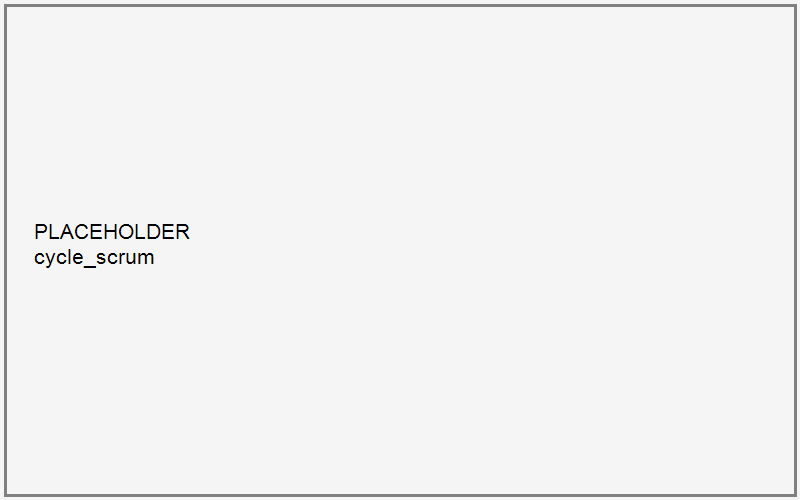
\includegraphics[width=12cm]{image/ChatGPT Image Aug 8, 2026, 07_07_47 PM.png}
    \caption{Cycle de travail Scrum adopté pour la conduite du projet}
    \label{fig:cycle-scrum}
\end{figure}

\subsection*{Organisation de l'équipe Scrum}

La méthodologie Scrum s'appuie sur trois rôles principaux :

\paragraph{Product Owner}\mbox{}\par
Le Product Owner représente les besoins des utilisateurs et définit la vision du produit. Il est chargé de gérer et de prioriser le backlog afin de maximiser la valeur du projet. Ses principales responsabilités sont :
\begin{itemize}
    \item Définir et prioriser les fonctionnalités ;
    \item Planifier les différentes releases ;
    \item Ajuster les priorités en fonction des besoins ;
    \item Valider les fonctionnalités développées.
\end{itemize}

\paragraph{Scrum Master}\mbox{}\par
Le Scrum Master veille au respect des principes Scrum et facilite la collaboration entre les membres de l'équipe. Il accompagne également l'équipe dans la résolution des obstacles pouvant ralentir le développement.

\paragraph{Équipe de développement}\mbox{}\par
L'équipe de développement est responsable de la conception, de l'implémentation et des tests des différentes fonctionnalités du système afin d'atteindre les objectifs fixés pour chaque sprint.

\subsection*{Répartition des rôles}

Dans le cadre de notre projet, les rôles Scrum sont répartis comme suit :
\begin{itemize}
    \item Product Owner : encadrant académique et encadrant professionnel au sein de NextStep IT ;
    \item Scrum Master : Arafet Ben Kilani ;
    \item Équipe de développement : Adel Bettaieb.
\end{itemize}

\subsection*{Planification dans Scrum}

La méthodologie Scrum s'appuie principalement sur trois concepts : le Sprint (période de développement durant laquelle un ensemble de fonctionnalités est réalisé), la Release (version du produit regroupant un ou plusieurs sprints validés), et le Weekly Scrum : compte tenu de l'organisation mono-développeur du projet, la réunion de suivi n'est pas tenue quotidiennement mais de façon hebdomadaire, permettant de suivre l'avancement des travaux, d'identifier les difficultés rencontrées et de coordonner les tâches à réaliser pour la semaine suivante.

\section{Conclusion}

Dans ce chapitre, nous avons présenté l'organisme d'accueil ainsi que le contexte général du projet. Nous avons ensuite exposé la problématique, étudié les solutions existantes et comparé plusieurs méthodologies de développement afin de justifier le choix de Scrum. Le chapitre suivant est consacré à l'analyse et la spécification des besoins de la plateforme.


\chapter{Analyse et spécification des besoins}

\section{Introduction}

Après avoir présenté, au chapitre précédent, le contexte général du projet ainsi que la solution retenue, ce chapitre a pour objectif de spécifier précisément les besoins auxquels la plateforme doit répondre, puis de fournir une vue d'ensemble de l'analyse globale du système et de son pilotage. Nous identifions dans un premier temps les différents acteurs qui interagissent avec le système, puis nous détaillons les besoins fonctionnels et non fonctionnels, ainsi que le diagramme de cas d'utilisation général. Nous présentons ensuite l'analyse globale de la plateforme (diagramme de classes d'analyse et architecture logique/physique), le pilotage du projet avec la méthode Scrum, avant de clore le chapitre par la description de l'environnement de travail utilisé pour la réalisation du projet.

\section{Modélisation du contexte}

\subsection{Identification des acteurs}

L'analyse de la documentation fonctionnelle de la plateforme permet d'identifier trois acteurs principaux, correspondant aux rôles gérés par le module de sécurité (Keycloak et couche d'autorisation applicative) :

\begin{itemize}[label=--]
\item Administrateur de la plateforme (ADMIN) : représente l'équipe opérationnelle de NextStep IT en charge de l'exploitation de la plateforme. Il supervise l'ensemble des clients (tenants), le cluster Kubernetes, la facturation globale, les quotas, et intervient via la console d'administration dédiée.

\item Administrateur de compte client (CLIENT\_ADMIN) : représente le responsable, côté client, d'un compte locataire de la plateforme. Il gère son équipe (invitation de membres), configure et déploie ses applications, consulte sa facturation, et dispose de la totalité des permissions sur les ressources de son compte.

\item Membre d'équipe (MEMBER) : utilisateur rattaché à un compte client, disposant d'un sous-ensemble de permissions accordées explicitement par le CLIENT\_ADMIN (par exemple : déployer une application, consulter les journaux, consulter la supervision, gérer Kafka ou l'Eventing), sans nécessairement disposer de l'ensemble des droits du compte.
\end{itemize}

\subsection{Spécification des besoins}
\label{sec:besoins-fonctionnels}

\medskip
\textbf{Besoins fonctionnels}
\medskip

Les besoins fonctionnels sont organisés ci-dessous selon les grands blocs fonctionnels et techniques de la plateforme, qui seront repris sous forme d'epics dans le Product Backlog présenté en section~\ref{sec:scrum}.

\begin{itemize}
    \item \textbf{Gestion des utilisateurs \& de l'authentification}
    \begin{itemize}[label=--]
        \item Inscription/connexion via Keycloak (SSO, OIDC).
        \item Modification du profil (email, mot de passe) synchronisée avec Keycloak.
    \end{itemize}

    \item \textbf{Gestion des déploiements d'applications}
    \begin{itemize}[label=--]
        \item Déployer une image Docker (Docker Hub ou registre privé) comme service serverless (Knative).
        \item Configuration : nom, image et tag, port, ressources CPU/RAM, réplicas minimum/maximum (scale-to-zero inclus).
        \item Suivi du statut en temps réel (RUNNING / SCALED\_TO\_ZERO / DEPLOYING / FAILED / SUSPENDED).
        \item Mise à jour d'une application (image, réplicas, ressources) et redéploiement.
        \item Retour (rollback) vers une révision antérieure.
        \item Suppression d'une application (libère les ressources Knative).
    \end{itemize}

    \item \textbf{Gestion de la messagerie Kafka \& de l'Eventing}
    \begin{itemize}[label=--]
        \item Création et gestion de sujets (topics) Kafka par tenant.
        \item Création de sources d'événements (KafkaSource) reliant un sujet à une application Knative.
        \item Création de déclencheurs (triggers Broker~$\rightarrow$~Subscriber) pour le routage d'événements CloudEvents.
    \end{itemize}

    \item \textbf{Gestion du monitoring \& des journaux}
    \begin{itemize}[label=--]
        \item Journaux de déploiement en temps réel (streaming SSE).
        \item Tableau de bord de métriques (CPU, RAM, requêtes/s) via Prometheus/Grafana.
        \item Alertes (échec de déploiement, boucle de redémarrage, dépassement de budget).
        \item Notifications in-app configurables par type d'événement.
    \end{itemize}

    \item \textbf{Gestion de la facturation \& du paiement}
    \begin{itemize}[label=--]
        \item Calcul du coût à l'usage (CPU-heure, RAM-heure) par application et par tenant.
        \item Génération automatique de factures mensuelles (1\textsuperscript{er} du mois).
        \item Paiement par carte bancaire (Stripe~\cite{StripeDoc}) — enregistrement de cartes, paiement de facture.
        \item Historique des transactions.
        \item Alerte J-3 avant échéance, passage automatique au statut OVERDUE en cas d'impayé.
        \item Suspension automatique du service en cas de facture impayée après échéance.
        \item Export du relevé de facturation (Excel).
    \end{itemize}

    \item \textbf{Gestion administrative (rôle ADMIN)}
    \begin{itemize}[label=--]
        \item Vue d'ensemble du cluster (nœuds, pods, namespaces, alertes actives).
        \item Gestion des clients : liste, suspension/restauration globale d'un compte.
        \item Gestion des quotas par tenant (CPU/RAM/nombre d'applications maximum) avec synchronisation des ResourceQuota Kubernetes.
        \item Gestion des applications tous tenants confondus (suppression forcée, suspension/restauration).
        \item Tableau de bord des revenus (facturation du mois en cours, projection de fin de mois, revenu par client, revenu Kafka).
        \item Génération manuelle des factures mensuelles (hors tâche planifiée).
        \item Suspension d'un service précis pour facture impayée.
        \item Journal d'audit des actions administratives (qui a fait quoi, quand), exportable en CSV.
    \end{itemize}
\end{itemize}

\medskip
\textbf{Besoins non fonctionnels}
\medskip

\begin{itemize}
    \item \textbf{Isolation multi-tenant}
    \begin{itemize}[label=--]
        \item Les ressources et les données d'un client ne doivent en aucun cas être accessibles par un autre client, ni par un tenant vers les composants internes de la plateforme (base de données, service d'authentification).
        \item Isolation au niveau applicatif : contrôle d'accès basé sur le propriétaire effectif de la ressource.
        \item Isolation au niveau réseau : règles d'isolation entre espaces de noms Kubernetes, appliquées automatiquement à la création de chaque namespace tenant.
        \item Isolation au niveau des droits d'accès au cluster : contrôle d'accès basé sur les rôles limitant le compte de service du backend aux seules ressources strictement nécessaires, secrets Kubernetes pour les identifiants sensibles.
    \end{itemize}

    \item \textbf{Élasticité et efficience des ressources}
    \begin{itemize}[label=--]
        \item Une application ne doit consommer aucune ressource de calcul lorsqu'elle est inactive (mise à l'échelle à zéro).
        \item La plateforme doit monter en charge automatiquement en fonction du trafic reçu, dans les bornes de réplicas configurées par le client.
        \item Le temps de réveil d'une application mise à l'échelle à zéro (cold start) doit rester acceptable pour l'utilisateur final.
    \end{itemize}

    \item \textbf{Sécurité}
    \begin{itemize}[label=--]
        \item L'authentification des utilisateurs doit reposer sur un fournisseur d'identité centralisé (Keycloak).
        \item Les autorisations doivent être vérifiées à chaque accès à une ressource, en fonction du rôle et du propriétaire effectif.
        \item Les échanges sensibles (jetons d'authentification, identifiants) ne doivent pas être exposés inutilement (journaux, paramètres d'URL, code source).
    \end{itemize}

    \item \textbf{Disponibilité}
    \begin{itemize}[label=--]
        \item Les composants de la plateforme elle-même (backend, portails, briques d'infrastructure) doivent pouvoir être redéployés sans interruption prolongée de service.
        \item Le système doit permettre de détecter automatiquement une dégradation (redémarrages en boucle, alertes) et, si possible, la corriger sans intervention manuelle.
    \end{itemize}

    \item \textbf{Observabilité}
    \begin{itemize}[label=--]
        \item L'état du système, à tous les niveaux (infrastructure, plateforme, applications clientes), doit pouvoir être supervisé au travers d'outils de métriques et de tableaux de bord (Prometheus/Grafana).
        \item Les journaux applicatifs et de déploiement doivent être consultables en temps réel.
        \item Les actions administratives sensibles doivent être tracées dans un journal d'audit consultable a posteriori.
    \end{itemize}

    \item \textbf{Automatisation}
    \begin{itemize}[label=--]
        \item La construction, la publication et le déploiement des composants de la plateforme doivent être automatisés à chaque évolution du code source.
        \item L'automatisation doit couvrir l'ensemble des composants déployables de la plateforme (backend, portail client, console d'administration).
    \end{itemize}
\end{itemize}

\subsection{Diagramme de cas d'utilisation général}
Dans cette section, nous décrivons les exigences du système de manière formelle à l'aide des deux diagrammes de cas d'utilisation ci-dessous (figures~\ref{fig:uc-global} et~\ref{fig:uc-global-admin}), qui couvrent respectivement les rôles CLIENT\_ADMIN/MEMBER et le rôle ADMIN.

\begin{figure}[H]
 \centering
    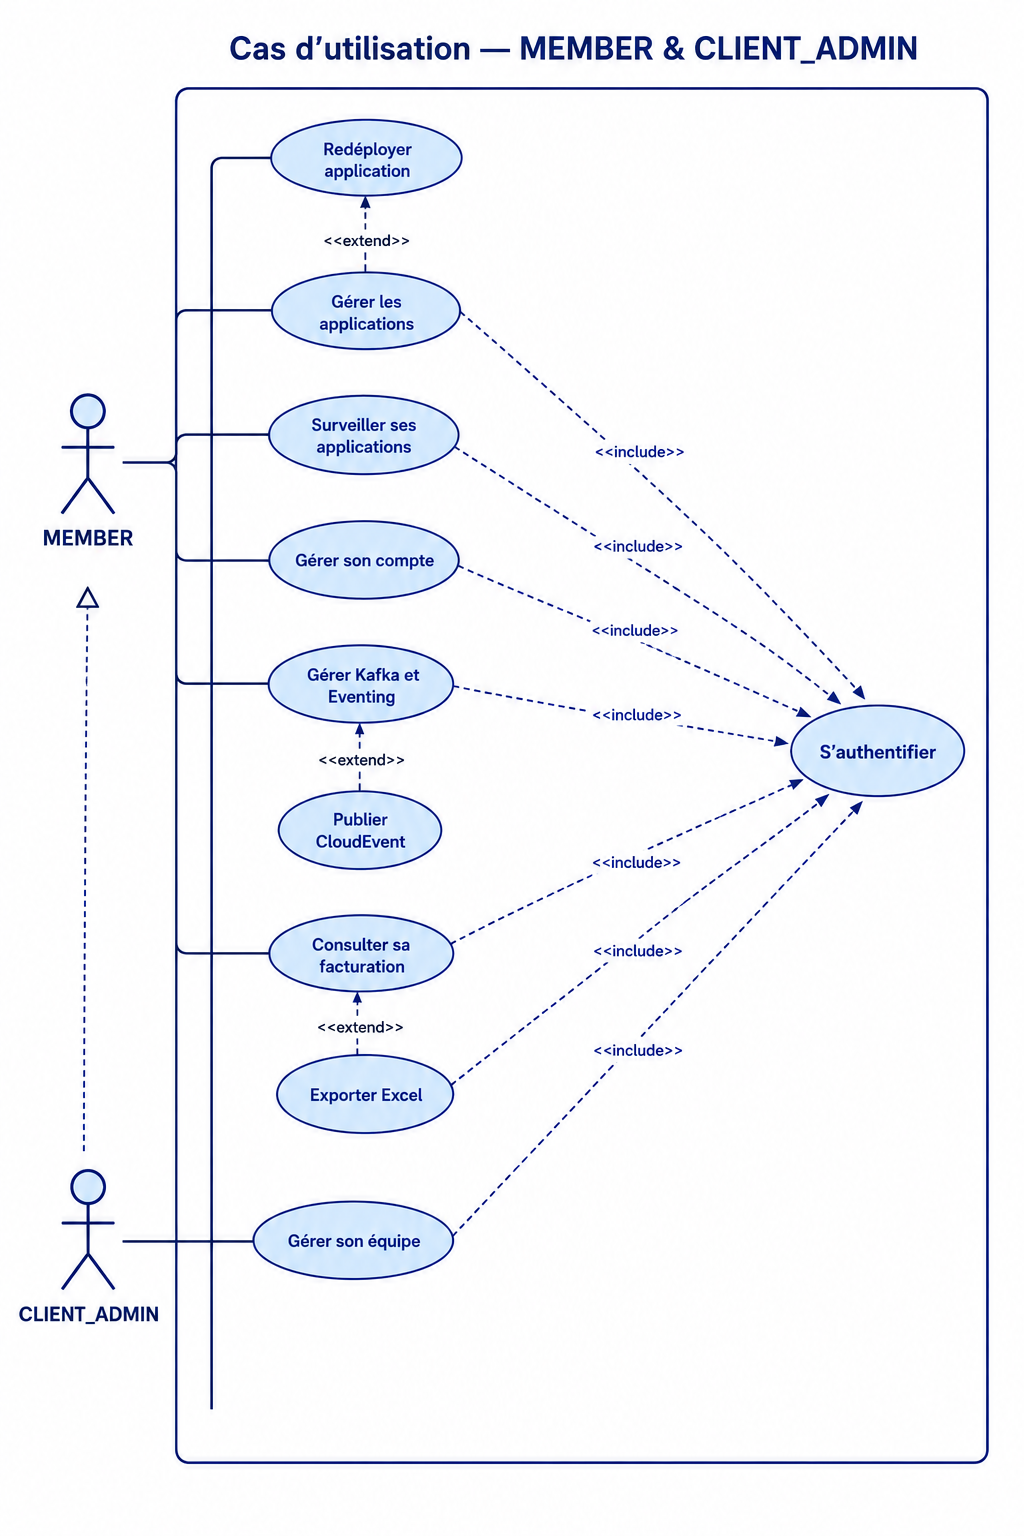
\includegraphics[width=13cm]{image/usescasememeberadmin.png}
    \caption{Diagramme de cas d'utilisation global de la plateforme — CLIENT\_ADMIN et MEMBER}
    \label{fig:uc-global}
\end{figure}

\begin{figure}[H]
 \centering
    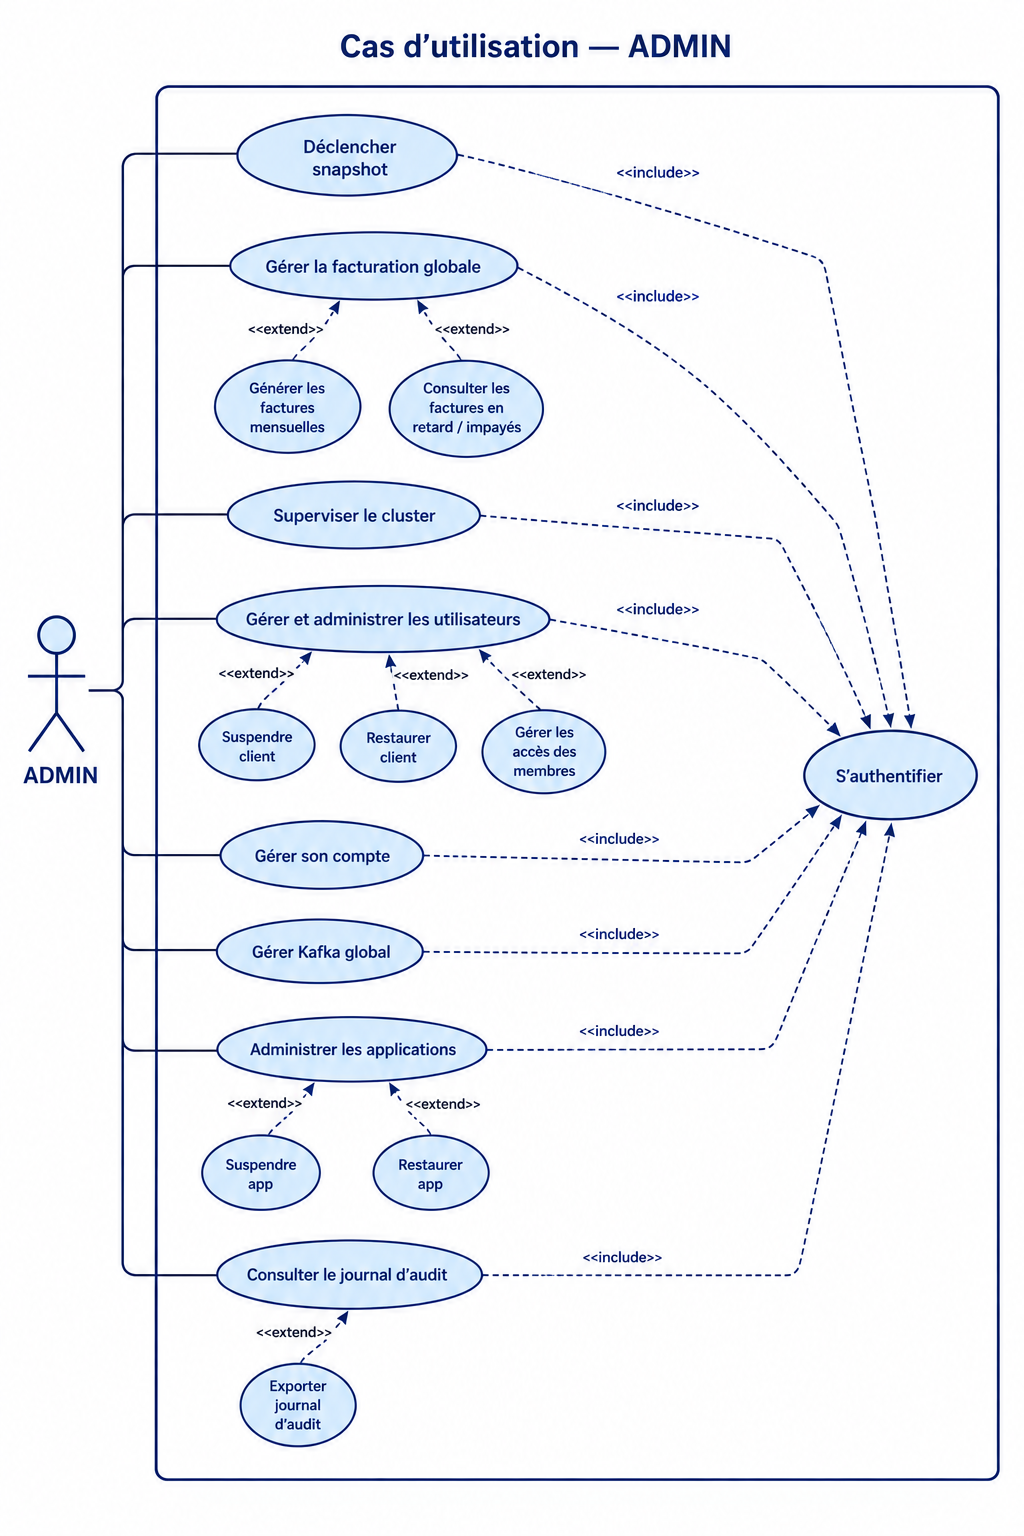
\includegraphics[width=13cm]{image/diagrameadmin.png}
    \caption{Diagramme de cas d'utilisation global de la plateforme — ADMIN}
    \label{fig:uc-global-admin}
\end{figure}

\section{Analyse Globale}

Cette section donne une vue d'ensemble cohérente de l'architecture logique et physique du système, des composants qui le constituent et de leurs interactions, ainsi que des processus métier les plus structurants, indépendamment du découpage en sprints qui structurera les chapitres suivants. Les diagrammes UML propres à une fonctionnalité particulière (par exemple le diagramme de séquence détaillé de la création d'un déclencheur Kafka) seront présentés dans le chapitre de réalisation correspondant, en cohérence avec la vue d'ensemble donnée ici.

\subsection{Diagramme de classes d'analyse}

La figure~\ref{fig:classes-global} présente les principales entités métier du système et leurs relations : \texttt{User}, \texttt{App}, \texttt{DeploymentLog}, \texttt{BillingSnapshot}, \texttt{AppInvoice} et les clés d'API. La propriété des applications est gérée par \texttt{UserContextService}, qui rattache les ressources d'un \texttt{MEMBER} à son \texttt{CLIENT\_ADMIN}.

\begin{figure}[H]
 \centering
    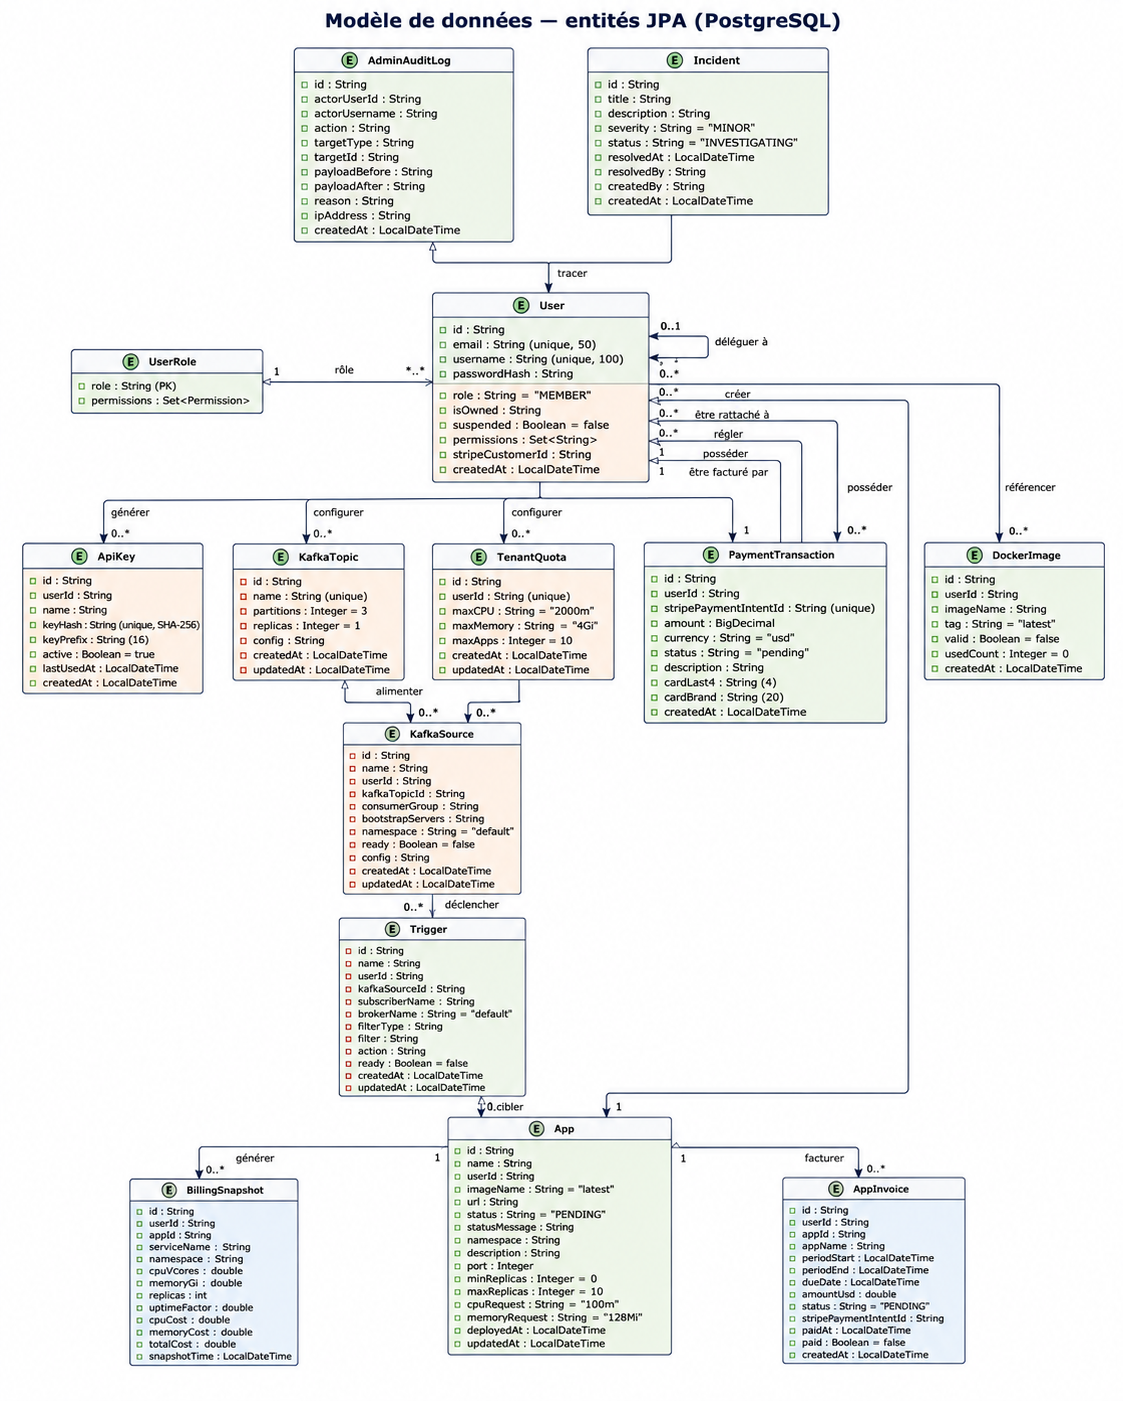
\includegraphics[width=13.5cm]{image/class1.png}
    \caption{Diagramme de classe d'analyse global}
    \label{fig:classes-global}
\end{figure}

\subsection{Architecture globale}

\subsubsection{Architecture logique de la plateforme}

L'architecture logique de la plateforme est organisée en trois couches, représentées à la figure ~\ref{fig:architecture-logique} :

\begin{figure}[H]
\centering
    
\includegraphics[width=13.5cm]{image/architecture_logique.png}
    \caption{Architecture logique de la plateforme}
    \label{fig:architecture-logique}
\end{figure}


\begin{itemize}
    \item \textbf{Présentation} : deux applications React distinctes, servies via Nginx. Le portail client couvre le déploiement et le suivi des applications, la facturation et la gestion d'équipe ; la console d'administration donne à l'équipe NextStep IT une vue sur l'ensemble des clients et du cluster.
    \item \textbf{Service} : une seule API REST en Spring Boot, découpée par domaine métier (applications, sécurité, Kafka, facturation, administration...). C'est elle qui concentre toute la logique et qui parle au cluster, via Fabric8 — une bibliothèque Java exécutée dans son propre processus, pas un service séparé.
    \item \textbf{Infrastructure} : le cluster Kubernetes et ses opérateurs (Knative pour l'exécution serverless, Strimzi pour Kafka), la couche réseau (Cilium en CNI, Kourier en passerelle d'entrée), et les briques transverses Keycloak, PostgreSQL, Prometheus/Grafana.
\end{itemize}

Seul le backend parle à l'API Kubernetes : ni les portails ni un système externe (un pipeline CI/CD, par exemple) n'y accèdent directement. Toute action passe donc par cette couche de service, qui applique l'authentification et l'isolation entre tenants avant d'agir sur le cluster.

\subsubsection{Architecture physique de la plateforme}

Au-delà de son organisation logique, il est utile de voir comment la plateforme se répartit concrètement sur le cluster une fois en fonctionnement. La figure~\ref{fig:archi-physique} reprend, namespace par namespace, ce qui a pu être observé directement sur le cluster décrit en section~\ref{sec:env-materiel} — les pods réellement en cours d'exécution, et non une simple projection théorique du déploiement.

\begin{figure}[H]
\centering
    
\includegraphics[width=13.5cm]{image/architecture_physique.png}
    \caption{Architecture physique de l'infrastructure Kubernetes}
    \label{fig:archi-physique}
\end{figure}

Le cluster s'appuie sur trois nœuds Ubuntu. \texttt{vm01} porte le plan de contrôle Kubernetes (\texttt{kube-apiserver}, \texttt{etcd}, \texttt{kube-scheduler}, \texttt{kube-controller-manager}), tandis que \texttt{vm02} et \texttt{vm03} font tourner l'ensemble des pods, ceux de la plateforme comme ceux des applications clientes.

En façade, trois composants réseau se partagent des rôles bien distincts. MetalLB attribue une adresse IP de type \texttt{LoadBalancer} à chaque \texttt{Service} Kubernetes qui en a besoin ; Kourier se contente de router le trafic HTTP vers les applications Knative des tenants ; Cilium, lui, assure la connectivité des pods en tant que CNI du cluster et applique les \texttt{NetworkPolicy}. Le backend et les portails, exposés directement en \texttt{Service} \texttt{LoadBalancer}, reçoivent donc leur IP de MetalLB sans jamais transiter par Kourier.

Le namespace \texttt{platform} regroupe les deux composants centraux de la plateforme : PostgreSQL, avec son volume persistant, et le backend Spring Boot. Ce dernier tourne en \texttt{Deployment} Kubernetes classique plutôt qu'en service Knative, car il doit rester disponible en permanence et ne se prête pas à une mise à l'échelle à zéro.

Vient ensuite le middleware Cloud Native. Le broker Kafka, opéré par Strimzi, est une instance unique du cluster, mutualisée entre tous les tenants. Il en va de même pour le plan de contrôle de Knative Eventing (le contrôleur Eventing et le dispatcher de sources Kafka), qui tourne une seule fois pour tout le cluster plutôt que d'être dupliqué par client — à la différence des ressources Broker et Trigger elles-mêmes, qui sont instanciées séparément dans le namespace de chaque tenant. Cette mutualisation du plan de contrôle a une conséquence concrète : lorsque le dispatcher de sources Kafka a connu un incident, la livraison d'événements s'est interrompue pour tous les clients à la fois, pas seulement pour l'un d'eux.

Enfin, chaque client dispose de son propre namespace \texttt{user-<client>}, créé automatiquement lors de son premier déploiement et isolé par une \texttt{NetworkPolicy} générée à la volée. C'est là que vivent ses applications, sous forme de ressources Knative Service donnant naissance à des Revisions puis à des pods applicatifs.

\section{Pilotage du projet avec SCRUM}
\label{sec:scrum}

Le cadre agile Scrum, retenu au chapitre précédent pour la conduite de ce projet, structure le développement en itérations courtes et fixes appelées sprints, à l'issue desquelles un incrément de produit potentiellement livrable est produit.

Dans les tableaux de backlog présentés dans ce chapitre et les suivants, chaque tâche est associée à une estimation exprimée sur une échelle de complexité relative à trois niveaux : \textbf{1} (faible complexité — modification simple ou localisée), \textbf{2} (complexité moyenne — développement impliquant plusieurs composants ou une logique métier non triviale) et \textbf{3} (complexité élevée — intégration de plusieurs systèmes, gestion d'états asynchrones ou risques techniques significatifs).

\subsection{Backlog du produit}

Le tableau~\ref{tab:backlog} présente le backlog du produit de la plateforme. Les fonctionnalités sont organisées par module (en cohérence directe avec les besoins fonctionnels spécifiés en section~\ref{sec:besoins-fonctionnels}) et décrites sous forme de User Stories.

{
\setlength{\tabcolsep}{4pt}
\renewcommand{\arraystretch}{1.5}
\begin{longtable}{|>{\centering\arraybackslash}m{1.1cm}|>{\centering\arraybackslash}m{2.9cm}|>{\centering\arraybackslash}m{1.4cm}|>{\raggedright\arraybackslash}p{6.6cm}|>{\centering\arraybackslash}m{2.3cm}|}
\hline
ID & Module & ID US & User Story & Complexité\\
\hline
\endfirsthead

\hline
ID & Module & ID US & User Story & Complexité\\
\hline
\endhead

\hline
\multicolumn{5}{r}{Suite à la page suivante}\\
\endfoot

\endlastfoot

\multirow{4}{*}{M1} & \multirow{4}{2.9cm}{\centering Authentification \& Sécurité} & M1.1 & En tant qu'ADMIN, CLIENT\_ADMIN ou MEMBER, je souhaite me connecter à la plateforme via Keycloak. & Moyenne\\
\cline{3-5}
&& M1.2 & En tant qu'ADMIN, CLIENT\_ADMIN ou MEMBER, je souhaite me déconnecter du système. & Faible\\
\cline{3-5}
&& M1.3 & En tant qu'ADMIN, CLIENT\_ADMIN ou MEMBER, je souhaite que mon jeton d'authentification (JWT) soit automatiquement rafraîchi. & Moyenne\\
\cline{3-5}
&& M1.4 & En tant qu'ADMIN, je souhaite définir les rôles et les permissions des utilisateurs. & Élevée\\
\hline

\multirow{4}{*}{M2} & \multirow{4}{2.9cm}{\centering Utilisateurs \& équipes} & M2.1 & En tant que CLIENT\_ADMIN, je souhaite inviter un membre dans mon équipe. & Moyenne\\
\cline{3-5}
&& M2.2 & En tant que CLIENT\_ADMIN, je souhaite modifier les permissions d'un membre de mon équipe. & Moyenne\\
\cline{3-5}
&& M2.3 & En tant que CLIENT\_ADMIN, je souhaite retirer un membre de mon équipe. & Faible\\
\cline{3-5}
&& M2.4 & En tant qu'ADMIN, je souhaite gérer les comptes clients (activation, suspension, quotas). & Élevée\\
\hline

\multirow{3}{*}{M3} & \multirow{3}{2.9cm}{\centering Infrastructure Cloud Native} & M3.1 & En tant que système, je souhaite créer automatiquement un espace de noms (namespace) dédié pour chaque nouveau tenant. & Élevée\\
\cline{3-5}
&& M3.2 & En tant que système, je souhaite appliquer automatiquement une NetworkPolicy isolant chaque tenant. & Élevée\\
\cline{3-5}
&& M3.3 & En tant qu'ADMIN, je souhaite superviser l'état des nœuds du cluster Kubernetes. & Moyenne\\
\hline

\multirow{1}{*}{M4} & \multirow{1}{2.9cm}{\centering Gestion des applications} & M4.1 & En tant que CLIENT\_ADMIN ou MEMBER, je souhaite déployer une application à partir d'une image Docker. & Élevée\\
\cline{3-5}
&& M4.2 & En tant que CLIENT\_ADMIN ou MEMBER, je souhaite définir les ressources (CPU, mémoire) et les bornes de mise à l'échelle de mon application. & Moyenne\\
\cline{3-5}
&& M4.3 & En tant que CLIENT\_ADMIN ou MEMBER, je souhaite mettre à jour la configuration d'une application déjà déployée. & Moyenne\\
\cline{3-5}
&& M4.4 & En tant que CLIENT\_ADMIN ou MEMBER, je souhaite supprimer une application (suppression logique, conservation de l'historique de facturation). & Moyenne\\
\cline{3-5}
&& M4.5 & En tant que CLIENT\_ADMIN ou MEMBER, je souhaite consulter l'historique des révisions d'une application. & Moyenne\\
\cline{3-5}
&& M4.6 & En tant que CLIENT\_ADMIN ou MEMBER, je souhaite effectuer un rollback vers une révision antérieure. & Élevée\\
\cline{3-5}
&& M4.7 & En tant que CLIENT\_ADMIN ou MEMBER, je souhaite suivre en temps réel le statut de déploiement de mon application. & Élevée\\
\hline

\multirow{3}{*}{M5} & \multirow{3}{2.9cm}{\centering Messaging Kafka} & M5.1 & En tant que CLIENT\_ADMIN ou MEMBER, je souhaite créer un sujet (topic) Kafka pour mon compte. & Moyenne\\
\cline{3-5}
&& M5.2 & En tant que CLIENT\_ADMIN ou MEMBER, je souhaite consulter la liste des sujets Kafka de mon compte. & Faible\\
\cline{3-5}
&& M5.3 & En tant que CLIENT\_ADMIN ou MEMBER, je souhaite supprimer un sujet Kafka. & Faible\\
\hline

\multirow{3}{*}{M6} & \multirow{3}{2.9cm}{\centering Knative Eventing} & M6.1 & En tant que CLIENT\_ADMIN ou MEMBER, je souhaite relier un sujet Kafka à une de mes applications déployées. & Élevée\\
\cline{3-5}
&& M6.2 & En tant que CLIENT\_ADMIN ou MEMBER, je souhaite que mon application soit automatiquement réveillée (scale depuis zéro) à la réception d'un événement. & Élevée\\
\cline{3-5}
&& M6.3 & En tant que CLIENT\_ADMIN ou MEMBER, je souhaite configurer un déclencheur (Trigger) avec un filtre sur le type d'événement. & Moyenne\\
\hline

\multirow{3}{*}{M7} & \multirow{3}{2.9cm}{\centering Facturation} & M7.1 & En tant que CLIENT\_ADMIN ou MEMBER, je souhaite consulter la facturation de mes applications basée sur leur usage réel. & Élevée\\
\cline{3-5}
&& M7.2 & En tant qu'ADMIN, je souhaite consulter la facturation globale de tous les comptes clients. & Moyenne\\
\cline{3-5}
&& M7.3 & En tant que CLIENT\_ADMIN ou MEMBER, je souhaite recevoir une alerte lorsque mon budget approche un seuil défini. & Moyenne\\
\hline

\multirow{4}{*}{M8} & \multirow{4}{2.9cm}{\centering Monitoring \& Observabilité} & M8.1 & En tant que CLIENT\_ADMIN ou MEMBER, je souhaite consulter les journaux applicatifs de mon application en temps réel (SSE). & Élevée\\
\cline{3-5}
&& M8.2 & En tant que CLIENT\_ADMIN ou MEMBER, je souhaite consulter les métriques (CPU, mémoire, requêtes) de mon application. & Moyenne\\
\cline{3-5}
&& M8.3 & En tant que CLIENT\_ADMIN ou MEMBER, je souhaite être alerté automatiquement en cas de redémarrage en boucle (crash loop) d'une application. & Élevée\\
\cline{3-5}
&& M8.4 & En tant qu'ADMIN, je souhaite consulter un tableau de bord Grafana de l'état global du cluster. & Moyenne\\
\hline

\multirow{2}{*}{M9} & \multirow{2}{2.9cm}{\centering Administration plateforme} & M9.1 & En tant qu'ADMIN, je souhaite consulter le journal d'audit des actions effectuées sur la plateforme. & Moyenne\\
\cline{3-5}
&& M9.2 & En tant qu'ADMIN, je souhaite gérer les quotas alloués à chaque compte client. & Moyenne\\
\hline

\multirow{3}{*}{M10} & \multirow{3}{2.9cm}{\centering CI/CD} & M10.1 & En tant qu'équipe de développement de la plateforme, je souhaite que chaque évolution du code source déclenche automatiquement la construction d'une image Docker via Kaniko. & Élevée\\
\cline{3-5}
&& M10.2 & En tant qu'équipe de développement de la plateforme, je souhaite que l'image construite soit automatiquement publiée sur le registre Docker Hub. & Moyenne\\
\cline{3-5}
&& M10.3 & En tant qu'équipe de développement de la plateforme, je souhaite que la nouvelle version soit automatiquement déployée sur le cluster après publication. & Élevée\\
\hline
\caption{Backlog du produit}
\label{tab:backlog}
\end{longtable}
}

\subsection{Planification des Sprints}

La planification cible retenue pour la conduite du projet, définissant l'ordre logique de construction des différentes briques de la plateforme, est présentée dans le tableau~\ref{tab:sprints}. Cette planification a servi de cadre méthodologique tout au long du projet ; elle reflète la démarche adoptée plutôt qu'un journal exhaustif et daté de chaque tâche réalisée, celui-ci n'ayant pas fait l'objet d'une documentation formelle systématique sprint par sprint.

\begin{table}[H]
\centering
\renewcommand{\arraystretch}{1.3}
\begin{tabular}{|p{3cm}|p{10cm}|}
\hline
Sprint & Objectif principal \\
\hline
Sprint 0  & Infrastructure Kubernetes \\
\hline
Sprint 1  & Knative Serving \\
\hline
Sprint 2  & Kafka \& Strimzi \\
\hline
Sprint 3  & Gestion des utilisateurs et des accès (backend + portail) \\
\hline
Sprint 4  & Gestion des applications (backend + portail) et début du pipeline CI/CD Backend \\
\hline
Sprint 5  & Gestion de la messagerie événementielle : Kafka et Knative Eventing (backend + portail) \\
\hline
Sprint 6  & Gestion de l'observabilité applicative (backend + portail) \\
\hline
Sprint 7  & Gestion de la facturation et des paiements (backend + portail) \\
\hline
Sprint 8  & Gestion des comptes clients, des quotas et de l'audit \\
\hline
Sprint 9  & Gestion de l'exploitation du cluster et du statut public \\
\hline
Sprint 10 & Durcissement et sécurité \\
\hline
Sprint 11 & Pipeline CI/CD complet \\
\hline
\end{tabular}
\caption{Planification des sprints du projet}
\label{tab:sprints}
\end{table}

Le détail de la réalisation de chacun de ces sprints (analyse, conception et implémentation) est présenté progressivement dans les chapitres suivants, regroupés par release. Conformément aux besoins fonctionnels spécifiés en section~\ref{sec:besoins-fonctionnels} (portail client et console d'administration comme composants à part entière de la plateforme, au même titre que le backend), chaque sprint à partir du Sprint 3 livre conjointement la brique backend et l'interface graphique correspondante, plutôt que de reporter l'ensemble du développement frontend à la fin du projet.

\section{Environnement de travail}

\subsection{Environnement matériel de développement}
\label{sec:env-materiel}

\subsubsection{Poste de développement}

Le développement de la plateforme (backend, portails web, manifestes Kubernetes) a été réalisé sur un poste de travail disposant des caractéristiques suivantes :

\begin{itemize}
    \item Modèle : Ordinateur portable MSI GF63 Thin 10SC
    \item Système d'exploitation : Windows 11 Pro (64 bits)
    \item Processeur : Intel(R) Core(TM) i7-10750H CPU @ 2.60GHz
    \item Mémoire RAM : 16 Go
    \item Stockage : 2 $\times$ SSD 512 Go (TEAM T253 512GB + Micron 2210 512GB), soit environ 1 To au total
\end{itemize}

\subsubsection{Cluster de déploiement (infrastructure Kubernetes)}

Le déploiement et l'exploitation de la plateforme se sont appuyés sur un cluster Kubernetes composé de trois machines virtuelles sous Ubuntu 24, administrées via un utilisateur \texttt{sysadmin} : un nœud de plan de contrôle (control-plane) et deux nœuds de travail (workers), sur lesquels sont exécutés l'ensemble des composants de la plateforme ainsi que les applications des clients.

\begin{table}[H]
\centering
\renewcommand{\arraystretch}{1.3}
\begin{tabular}{|l|p{4cm}|c|p{5cm}|}
\hline
\textbf{Nom de la VM} & \textbf{Ressources} & \textbf{Système} & \textbf{Rôle} \\
\hline
Master   & 4 vCPU, 8 Go RAM, 50 Go disque & Ubuntu 24 & Plan de contrôle (control-plane) \\
\hline
Worker 1 & 4 vCPU, 8 Go RAM, 50 Go disque & Ubuntu 24 & Nœud de travail \\
\hline
Worker 2 & 4 vCPU, 8 Go RAM, 50 Go disque & Ubuntu 24 & Nœud de travail \\
\hline
\end{tabular}
\caption{Caractéristiques des machines virtuelles du cluster Kubernetes}
\label{tab:vms-cluster}
\end{table}

Le cluster utilise Cilium comme interface réseau de conteneurs (CNI), MetalLB pour l'attribution d'adresses IP aux services de type LoadBalancer dans un environnement dépourvu de répartiteur de charge natif, et Kourier comme passerelle d'entrée (ingress gateway) pour Knative Serving.

\subsection{Environnement logiciel de développement}

\subsubsection{Langages de programmation}

Le choix des langages de programmation est basé sur les exigences techniques de la plateforme : performance et sécurité du backend, réactivité des interfaces web, et portabilité des scripts d'exploitation du cluster. Le tableau~\ref{tab:langages} présente les langages utilisés.

\renewcommand{\arraystretch}{1.3}
\begin{center}
\begin{tabular}{|m{3cm}|m{10cm}|}
\hline
\centering Langage & \centering\arraybackslash Description \\
\hline
Java & Langage principal du backend applicatif (\texttt{backend-api}), développé avec Spring Boot. \\
\hline
TypeScript / JavaScript & Langages utilisés pour le développement des deux portails web React (\texttt{web-portal} et \texttt{admin-console}). \\
\hline
YAML & Langage de description déclarative utilisé pour l'ensemble des manifestes Kubernetes, Knative, Strimzi, ainsi que pour la configuration de l'application (\texttt{application.yml}). \\
\hline
Shell (Bash) & Utilisé pour les scripts de déploiement, d'initialisation du cluster et d'automatisation des tâches d'exploitation. \\
\hline
Groovy & Langage utilisé pour l'écriture des Jenkinsfiles du pipeline CI/CD. \\
\hline
\end{tabular}
\captionof{table}{Langages de programmation utilisés}
\label{tab:langages}
\end{center}

\vspace{1em}

\subsubsection{Frameworks et bibliothèques}

Les frameworks et bibliothèques retenus ont été sélectionnés pour leur maturité, leur performance et leur adéquation aux besoins fonctionnels de la plateforme. Le tableau~\ref{tab:frameworks} en présente une synthèse.

\renewcommand{\arraystretch}{1.3}
\begin{center}
\begingroup
\centering
\renewcommand{\arraystretch}{1.2}
\begin{longtable}{|m{3cm}|m{11.5cm}|}
\caption{Frameworks et bibliothèques utilisés}
\label{tab:frameworks}\\
\hline
\multicolumn{1}{|c|}{\textbf{Framework}} & \multicolumn{1}{c|}{\textbf{Description}} \\
\hline
\endfirsthead

\multicolumn{2}{l}{\small\itshape (suite du tableau~\ref{tab:frameworks})}\\
\hline
\multicolumn{1}{|c|}{\textbf{Framework}} & \multicolumn{1}{c|}{\textbf{Description}} \\
\hline
\endhead

\hline
\multicolumn{2}{r}{\small\itshape (suite page suivante)}\\
\endfoot

\hline
\endlastfoot

Spring Boot & Framework backend utilisé pour l'exposition de l'API REST, l'injection de dépendances, la sécurité (Spring Security) et l'accès aux données (Spring Data JPA). \\
\hline
Fabric8 Kubernetes Client & Bibliothèque Java utilisée par le backend pour orchestrer les ressources Kubernetes natives et les ressources personnalisées (CRD) de Knative Serving, Knative Eventing et Strimzi. \\
\hline
Kafka Clients (Apache Kafka) & Bibliothèque cliente utilisée par le backend (API Admin Kafka) pour créer et gérer les sujets (topics) des tenants. \\
\hline
React & Bibliothèque utilisée pour le développement des interfaces graphiques du portail client et de la console d'administration. \\
\hline
PostgreSQL / JPA-Hibernate & Système de gestion de base de données relationnelle et couche de mapping objet-relationnel utilisés pour la persistance des entités métier. \\
\hline
Keycloak (OpenID Connect) & Bibliothèque d'intégration utilisée côté backend et frontend pour l'authentification et la validation des jetons JWT. \\
\hline
\end{longtable}
\endgroup
\end{center}

\vspace{1em}

\subsubsection{Outils de développement et de modélisation}

Le tableau~\ref{tab:outils-dev} présente les outils utilisés pour l'écriture du code, la gestion de versions, les tests manuels d'API et la modélisation UML du présent mémoire.

\begingroup
\centering
\renewcommand{\arraystretch}{1.2}
\begin{longtable}{|m{3cm}|m{11.5cm}|}
\caption{Outils de développement et de modélisation utilisés}
\label{tab:outils-dev}\\
\hline
\multicolumn{1}{|c|}{\textbf{Outil}} & \multicolumn{1}{c|}{\textbf{Description}} \\
\hline
\endfirsthead

\multicolumn{2}{l}{\small\itshape (suite du tableau~\ref{tab:outils-dev})}\\
\hline
\multicolumn{1}{|c|}{\textbf{Outil}} & \multicolumn{1}{c|}{\textbf{Description}} \\
\hline
\endhead

\hline
\multicolumn{2}{r}{\small\itshape (suite page suivante)}\\
\endfoot

\hline
\endlastfoot

Visual Studio Code & Environnement de développement intégré léger et extensible, utilisé pour le développement du backend Spring Boot, des deux applications frontend React, ainsi que pour la rédaction des manifestes Kubernetes et des scripts de déploiement. \\
\hline
GitHub & Plateforme d'hébergement du code source et de gestion de versions, utilisée pour le suivi des évolutions du projet et le déclenchement des pipelines d'intégration continue. \\
\hline
Postman & Outil de test et de documentation des API REST, utilisé pour valider manuellement le comportement des différents points d'accès exposés par le backend avant leur intégration dans les interfaces graphiques. \\
\hline
PlantUML~\cite{PlantUMLDoc} & Outil de modélisation UML en tant que code, utilisé pour la production des diagrammes de cas d'utilisation, de classes, de composants, de déploiement et de séquence présentés dans ce mémoire, à partir de scripts textuels versionnés avec le code source. \\
\hline
\end{longtable}
\endgroup

\vspace{1em}

\subsubsection{Outils DevOps et déploiement}

La mise en production de la plateforme repose sur une chaîne DevOps automatisée garantissant la fiabilité et la répétabilité des déploiements. Le tableau~\ref{tab:outils-devops} présente les outils utilisés pour la conteneurisation, l'intégration continue et l'exploitation du cluster.

\renewcommand{\arraystretch}{1.3}

\begingroup
\centering
\renewcommand{\arraystretch}{1.2}
\begin{longtable}{|m{3cm}|m{11.5cm}|}
\caption{Outils DevOps et de déploiement utilisés}
\label{tab:outils-devops}\\
\hline
\multicolumn{1}{|c|}{\textbf{Outil}} & \multicolumn{1}{c|}{\textbf{Description}} \\
\hline
\endfirsthead

\multicolumn{2}{l}{\small\itshape (suite du tableau~\ref{tab:outils-devops})}\\
\hline
\multicolumn{1}{|c|}{\textbf{Outil}} & \multicolumn{1}{c|}{\textbf{Description}} \\
\hline
\endhead

\hline
\multicolumn{2}{r}{\small\itshape (suite page suivante)}\\
\endfoot

\hline
\endlastfoot

Docker & Utilisé pour la construction et l'exécution locale des images de conteneurs avant leur publication sur le registre Docker Hub par la chaîne CI/CD. \\
\hline
Jenkins et Kaniko & Utilisés pour l'automatisation de la construction, de la publication et du déploiement continu des composants de la plateforme, Kaniko permettant de construire les images sans démon Docker privilégié à l'intérieur du cluster. \\
\hline
kubectl & Interface en ligne de commande de Kubernetes, utilisée quotidiennement pour l'inspection de l'état du cluster, le déploiement manuel de ressources lors des phases de mise au point, et le diagnostic des incidents. \\
\hline
\end{longtable}
\endgroup
\section{Conclusion}

Ce chapitre a permis de formaliser les besoins fonctionnels et non fonctionnels de la plateforme, de préciser les acteurs qui interagissent avec le système et le diagramme de cas d'utilisation général qui en découle, puis de présenter l'analyse globale de la plateforme (diagramme de classes, architecture logique et physique, processus métier principaux) et le pilotage du projet au travers du Product Backlog et de la planification des sprints selon la méthode Scrum. L'environnement de travail matériel et logiciel utilisé pour la réalisation du projet a également été détaillé. Le détail de chaque sprint (description textuelle des cas d'utilisation, diagrammes de séquence spécifiques, réalisation) est développé progressivement dans les chapitres suivants, regroupés par release.


\chapter{Release 0 : Mise en place de la plateforme Cloud Native}

\section{Introduction}

La Release 0 constitue le socle technique du projet : trois sprints (Sprint 0, 1, 2) mettent en place les briques d'infrastructure cloud native — cluster Kubernetes, mise à l'échelle serverless via Knative Serving, bus d'événements Kafka opéré par Strimzi — sur lesquelles s'appuient la logique métier et les interfaces des releases suivantes.

Aucune de ces briques n'expose de fonctionnalité à un utilisateur final ; les sprints de cette release ne comportent donc pas de diagramme de cas d'utilisation. Le Chapitre II a présenté l'architecture cible de la plateforme ; ce chapitre documente comment chaque brique a été construite et validée, sprint après sprint.


\section{Sprint 0 : Mise en place de l'infrastructure Kubernetes}

\subsection{Introduction}

Le premier sprint porte sur le socle capable d'accueillir des charges de travail : un cluster Kubernetes à trois nœuds, un plugin réseau (CNI) appliquant l'isolation entre tenants, un mécanisme d'attribution d'adresses IP externes puisque le cluster n'est hébergé chez aucun fournisseur cloud, et une passerelle d'entrée prête pour les applications Knative du sprint suivant. Aucune de ces briques n'est visible pour un utilisateur, mais les choix faits ici, en particulier celui du plugin réseau, se répercutent jusqu'au modèle d'isolation multi-tenant de la plateforme.

\subsection{Objectifs du Sprint}

\begin{itemize}
    \item Mettre en place un cluster Kubernetes à trois nœuds opérationnels, à l'état Ready.
    \item Configurer un réseau de conteneurs (CNI) capable d'appliquer des règles NetworkPolicy entre espaces de noms.
    \item Isoler le trafic réseau entre les futurs tenants de la plateforme.
    \item Attribuer des adresses IP externes aux services LoadBalancer, le cluster n'étant pas hébergé chez un fournisseur cloud.
    \item Mettre en place la passerelle d'entrée Kourier, qui recevra le trafic vers les applications Knative à partir du Sprint 1.
    \item Définir la convention des espaces de noms, un par tenant et un pour la plateforme, ainsi que la convention d'adressage des applications.
\end{itemize}

La plateforme utilise une convention de nommage de la forme <app>.<namespace>.<ip-cluster>.sslip.io. L'adresse IP du cluster est intégrée directement dans le nom d'hôte, et sslip.io la résout automatiquement, sans zone DNS locale à administrer. Ce choix convient à un cluster on-premise en développement, au prix d'une URL moins lisible qu'un domaine dédié.

\subsection{Sprint Backlog}
Le tableau~\ref{tab:sb-sprint0} présente le backlog détaillé du Sprint 0, obtenu en décomposant chaque User Story retenue en tâches techniques.

{
% Le tableau deborde volontairement de 1,5 cm dans chaque marge afin de laisser
% respirer les trois colonnes ; LTleft/LTright sont les parametres propres a
% longtable (adjustwidth n'a aucun effet sur cet environnement).
% Largeur totale : 18,8 cm, soit 1 cm de blanc conserve de chaque cote de la page.
\setlength{\LTleft}{-1.5cm}
\setlength{\LTright}{-1.5cm}
\setlength{\tabcolsep}{8pt}
\renewcommand{\arraystretch}{1.9}
\begin{longtable}{|p{6.6cm}|>{\raggedright\arraybackslash}p{8.1cm}|>{\centering\arraybackslash}p{2.3cm}|}
\hline
User Story & Tâches & Estimation \\
\hline
\endfirsthead
\hline
User Story & Tâches & Estimation \\
\hline
\endhead
\endfoot
\hline
\caption{Backlog du Sprint 0}
\label{tab:sb-sprint0}
\endlastfoot

\multirow{4}{6.6cm}{
\centering
En tant qu'ADMIN, je veux disposer d'un cluster Kubernetes opérationnel afin d'héberger les composants de la plateforme.
}
&
Provisionner le cluster Kubernetes composé d'un control-plane et de deux workers.
& 2 \\*
\cline{2-3}
&
Configurer les nœuds et vérifier leur intégration au cluster.
& 1 \\*
\cline{2-3}
&
Vérifier l'état des trois nœuds et leur disponibilité pour l'exécution des workloads.
& 1 \\*
\cline{2-3}
&
Mettre en place les namespaces nécessaires à l'organisation des workloads et des tenants.
& 1 \\
\hline

\multirow{1}{6.6cm}{
\centering
En tant qu'ADMIN, je veux assurer la connectivité et l'isolation réseau entre les tenants.
}
&
Installer et configurer Cilium comme CNI du cluster Kubernetes.
& 2 \\*
\hline
\cline{2-3}
&
Vérifier le fonctionnement du réseau entre les workloads Kubernetes.
& 1 \\*
\cline{2-3}
&
Définir une politique réseau restrictive de type default-deny pour les namespaces tenants.
& 2 \\*
\cline{2-3}
&
Vérifier l'isolation réseau entre deux namespaces de tenants.
& 2 \\
\hline

\multirow{3}{6.6cm}{
\centering
En tant qu'ADMIN, je veux exposer les services Kubernetes vers le réseau externe.
}
&
Installer et configurer MetalLB dans le cluster on-premise.
& 2 \\*
\cline{2-3}
&
Configurer le mécanisme d'attribution des adresses IP externes aux services de type LoadBalancer.
& 2 \\*
\cline{2-3}
&
Vérifier l'attribution d'une adresse IP externe à un service Kubernetes.
& 1 \\
\hline

\multirow{3}{6.6cm}{
\centering
En tant qu'ADMIN, je veux une passerelle pour les futures applications Knative.
}
&
Installer Kourier comme passerelle d'entrée pour Knative Serving.
& 2 \\*
\cline{2-3}
&
Exposer le service Kourier à l'extérieur du cluster.
& 1 \\*
\cline{2-3}
&
Vérifier l'accessibilité de la passerelle depuis le réseau externe.
& 1 \\
\hline
\end{longtable}
}
% \subsection{Sprint Backlog}

% Le tableau~\ref{tab:sb-sprint0} présente le backlog détaillé du Sprint 0, obtenu en décomposant chaque User Story retenue en tâches techniques.

% % \needspace garantit qu'il reste assez de place sur la page : sans cela une
% % coupure peut tomber au milieu d'un groupe \multirow, dont le contenu deborde
% % alors hors du cadre et laisse une cellule vide sur la page suivante.
% \needspace{0.75\textheight}
% {
% % Le tableau deborde volontairement de 1,5 cm dans chaque marge afin de laisser
% % respirer les trois colonnes ; LTleft/LTright sont les parametres propres a
% % longtable (adjustwidth n'a aucun effet sur cet environnement).
% % Largeur totale : 18,8 cm, soit 1 cm de blanc conserve de chaque cote de la page.
% \setlength{\LTleft}{-1.5cm}
% \setlength{\LTright}{-1.5cm}
% \setlength{\tabcolsep}{8pt}
% \renewcommand{\arraystretch}{1.9}
% \begin{longtable}{|p{6.6cm}|>{\raggedright\arraybackslash}p{8.1cm}|>{\centering\arraybackslash}p{2.3cm}|}
% \hline
% User Story & Tâches & Estimation \\
% \hline
% \endfirsthead
% \hline
% User Story & Tâches & Estimation \\
% \hline
% \endhead
% \endfoot
% \hline

% \caption{Backlog du Sprint 0}
% \label{tab:sb-sprint0}
% \endlastfoot

% \multirow{4}{6.6cm}{
% \centering
% En tant qu'ADMIN, je veux disposer d'un cluster Kubernetes opérationnel afin d'héberger les composants de la plateforme.
% }
% &
% Provisionner le cluster Kubernetes composé d'un control-plane et de deux workers.
% & 2 \\
% \cline{2-3}

% &
% Configurer les nœuds et vérifier leur intégration au cluster.
% & 1 \\
% \cline{2-3}

% &
% Vérifier l'état des trois nœuds et leur disponibilité pour l'exécution des workloads.
% & 1 \\
% \cline{2-3}

% &
% Mettre en place les namespaces nécessaires à l'organisation des workloads et des tenants.
% & 1 \\
% \hline

% \multirow{4}{6.6cm}{
% \centering
% En tant qu'ADMIN, je veux assurer la connectivité et l'isolation réseau entre les tenants.
% }
% &
% Installer et configurer Cilium comme CNI du cluster Kubernetes.
% & 2 \\
% \cline{2-3}

% &
% Vérifier le fonctionnement du réseau entre les workloads Kubernetes.
% & 1 \\
% \cline{2-3}

% &
% Définir une politique réseau restrictive de type default-deny pour les namespaces tenants.
% & 2 \\
% \cline{2-3}

% &
% Vérifier l'isolation réseau entre deux namespaces de tenants.
% & 2 \\
% \hline

% \multirow{3}{6.6cm}{
% \centering
% En tant qu'ADMIN, je veux exposer les services Kubernetes vers le réseau externe.
% }
% &
% Installer et configurer MetalLB dans le cluster on-premise.
% & 2 \\
% \cline{2-3}

% &
% Configurer le mécanisme d'attribution des adresses IP externes aux services de type LoadBalancer.
% & 2 \\
% \cline{2-3}

% &
% Vérifier l'attribution d'une adresse IP externe à un service Kubernetes.
% & 1 \\
% \hline

% \multirow{1}{6.6cm}{
% \centering
% En tant qu'ADMIN, je veux une passerelle pour les futures applications Knative.
% }
% &
% Installer Kourier comme passerelle d'entrée pour Knative Serving.
% & 2 \\
% \hline
% \cline{2-3}

% &
% Exposer le service Kourier à l'extérieur du cluster.
% & 1 \\
% \cline{2-3}

% &
% Vérifier l'accessibilité de la passerelle depuis le réseau externe.
% & 1 \\
% \hline

% \end{longtable}
% }

\subsection{Conception}

\subsubsection{Rôle de Kubernetes et choix d'un cluster on-premise}

Construire une plateforme capable d'exécuter les applications de plusieurs clients sans qu'ils interfèrent entre eux suppose un socle d'orchestration de conteneurs : c'est le rôle de Kubernetes \cite{KubernetesDoc}, qui automatise le placement, le redémarrage et la mise à l'échelle des conteneurs sur un ensemble de machines, en s'appuyant sur le cloisonnement par namespace pour isoler les ressources d'un même cluster.

Ce cloisonnement par namespace est le mécanisme sur lequel repose toute la multi-tenance de la plateforme : chaque client obtient son propre namespace, isolé des autres clients et de la plateforme elle-même. La version exacte de Kubernetes et du container runtime utilisés n'est pas documentée de façon fiable dans le dépôt et n'est donc pas mentionnée ici.

\begin{itemize}
    \item \textbf{Choix d'un cluster on-premise :}\\
    - La plateforme est hébergée sur un cluster bare-metal propre à NextStep IT, plutôt que sur un service Kubernetes managé (EKS, GKE, AKS), cohérent avec les domaines Infrastructure as a Service et Hébergement/Housing de l'intégrateur (cf. Chapitre I), qui dispose ainsi de sa propre infrastructure sans dépendre d'un fournisseur cloud externe. Ce choix justifie directement la nécessité de MetalLB (section~\ref{sec:metallb}), qu'un cluster managé fournirait nativement.
\end{itemize}

\subsubsection{Architecture du cluster de la plateforme}

Le cluster utilisé pour le développement et l'exploitation de la plateforme compte trois nœuds : un nœud de plan de contrôle (control-plane) et deux nœuds de travail (workers). La répartition des rôles et les adresses IP, confirmées par la configuration réseau du backend (notamment sa liste blanche CORS), sont présentées à la figure~\ref{fig:cluster-topology}, qui illustre également la séparation logique entre l'espace de noms de la plateforme et ceux des tenants.

Les caractéristiques matérielles et le système d'exploitation de chaque nœud ne sont pas documentés de façon fiable. Un audit technique réalisé après une première mise en exploitation confirme cette topologie ainsi que la chaîne CNI, LoadBalancer et Ingress décrite dans ce chapitre.

\begin{figure}[H]
\begin{adjustwidth}{-1.0cm}{-1.0cm}
\centering
\begin{tikzpicture}[
  x=1cm, y=1cm,
  every node/.style={font=\normalsize},
  vm/.style={draw=figVert, line width=1pt, rounded corners, minimum width=4.2cm,
             minimum height=1.6cm, align=center, fill=figVertFond},
  cp/.style={draw=figVert, line width=1.4pt, rounded corners, minimum width=4.2cm,
             minimum height=1.6cm, align=center, fill=figVertFond!60!white},
  nsp/.style={draw=figBleu, line width=1pt, rounded corners, minimum width=6.4cm,
              minimum height=2.7cm, align=center, fill=figBleuFond},
  nst/.style={draw=figOrange, line width=1pt, dashed, rounded corners, minimum width=6.4cm,
              minimum height=2.7cm, align=center, fill=figOrangeFond},
  couche/.style={draw=black!40, dotted, line width=0.9pt, rounded corners, inner sep=12pt},
  ttl/.style={font=\small\bfseries, text=black!65}
]

% ---- couche physique : le plan de controle au centre, une liaison droite vers chaque worker ----
\node[vm] (vm02) at (0,0)    {vm02\\[1pt]\small worker\\\small 10.9.21.224};
\node[cp] (vm01) at (6.2,0)  {vm01\\[1pt]\small plan de contrôle\\\small 10.9.21.223};
\node[vm] (vm03) at (12.4,0) {vm03\\[1pt]\small worker\\\small 10.9.21.225};

\draw[<->, line width=1pt, figVert] (vm02) -- (vm01)
      node[midway, above=0pt, font=\scriptsize, fill=white, inner sep=1.5pt] {API Kubernetes};
\draw[<->, line width=1pt, figVert] (vm01) -- (vm03)
      node[midway, above=0pt, font=\scriptsize, fill=white, inner sep=1.5pt] {API Kubernetes};

\node[couche, fit=(vm02)(vm01)(vm03)] (phys) {};
\node[ttl, anchor=south west] at ([yshift=3pt]phys.north west) {Couche physique : trois nœuds};

% ---- couche logique : partition en namespaces ----
\node[nsp] (plat) at (2.6,-6.2)
     {Namespace \texttt{platform}\\[4pt]
      \small backend-api \quad web-portal\\\small admin-console\\\small PostgreSQL \quad Keycloak};
\node[nst] (ten) at (10.6,-6.2)
     {Namespace \texttt{user-<tenant>}\\[4pt]
      \small applications du client\\\small NetworkPolicy default-deny\\[2pt]
      \footnotesize\itshape un namespace par client, créé à la volée};

\node[couche, fit=(plat)(ten)] (logi) {};
\node[ttl, anchor=south west] at ([yshift=3pt]logi.north west) {Couche logique : namespaces};

% ---- articulation entre les deux couches ----
\draw[->, line width=1pt, black!55] (6.2,-1.9) -- (6.2,-3.6);
\node[font=\scriptsize, text=black!70, align=left, anchor=west] at (6.6,-2.75)
     {les Pods d'un namespace s'exécutent indifféremment\\sur \texttt{vm02} ou \texttt{vm03} : la répartition est logique,\\pas physique};

\end{tikzpicture}
\caption{Architecture du cluster Kubernetes de la plateforme}
\label{fig:cluster-topology}
\end{adjustwidth}
\end{figure}

Le namespace \texttt{user-<tenant>}, créé dynamiquement pour chaque client, contient ses applications déployées ainsi qu'une règle d'isolation réseau, détaillée ci-après.

\subsubsection{Isolation réseau des tenants : le CNI et Cilium}

Isoler des namespaces sur le papier ne suffit pas : il faut que le réseau du cluster respecte réellement cette séparation. Kubernetes délègue cette responsabilité à un plugin CNI (Container Network Interface), chargé d'attribuer une adresse IP à chaque Pod et d'acheminer le trafic.

Le CNI retenu est Cilium \cite{CiliumDoc}, choisi pour sa prise en charge des NetworkPolicy et son architecture eBPF, plus performante que les règles iptables traditionnelles et ouverte vers de l'observabilité réseau avancée. Comparé à Flannel, qui ne supporte pas nativement les NetworkPolicy, et à Calico, qui les supporte de façon comparable, Cilium a été retenu pour ce potentiel d'évolution. Un audit technique de la plateforme confirme ce choix comme robuste.

\paragraph{La NetworkPolicy réelle du projet.}\mbox{}\par
Une politique réseau de type default-deny (\texttt{k8s/tenant/network-policy.yaml}) est créée automatiquement pour chaque nouveau namespace tenant par le backend applicatif, un mécanisme détaillé au chapitre consacré à son développement (Release 1). Elle bloque par défaut tout trafic non explicitement autorisé entre Pods, et n'ouvre sélectivement que les flux nécessaires au fonctionnement de la plateforme : composants système (Kourier, Knative Serving, monitoring), résolution DNS, et bus d'événements Kafka partagé. Le trafic direct entre deux tenants reste refusé par défaut, garantissant qu'un client ne peut pas atteindre les ressources d'un autre, même en connaissant son adresse interne. La figure~\ref{fig:cilium-isolation} illustre ce principe.

\begin{figure}[H]
 \centering
    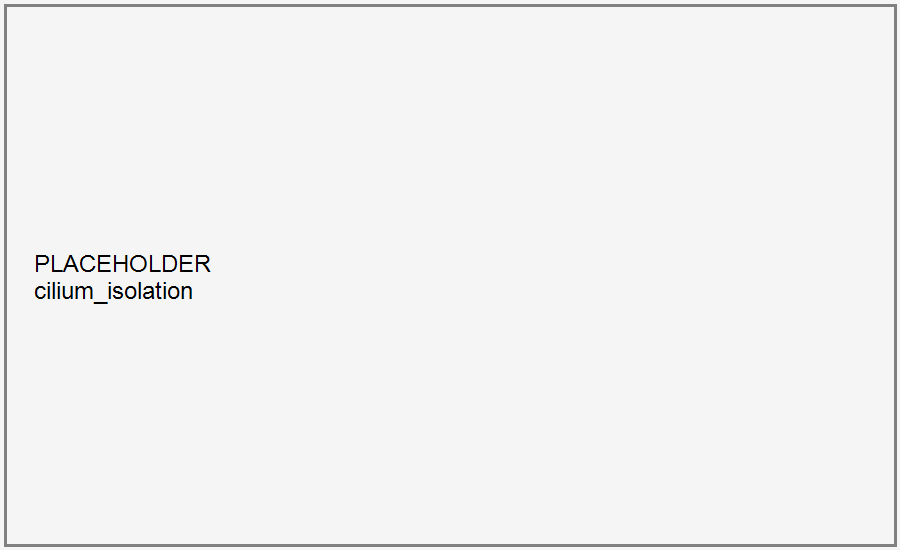
\includegraphics[width=0.85\textwidth]{image/cilium_isolation.png}
    \caption{Isolation réseau entre tenants via Cilium}
    \label{fig:cilium-isolation}
\end{figure}

\subsubsection{Exposition externe des services : MetalLB}
\label{sec:metallb}

Sur un cluster hébergé chez un fournisseur cloud public, un service LoadBalancer reçoit automatiquement une adresse IP publique — un mécanisme absent d'un cluster on-premise, où un tel service resterait indéfiniment à l'état \texttt{pending}. MetalLB \cite{MetalLBDoc} comble ce manque en attribuant, depuis l'intérieur du cluster, des adresses IP externes puisées dans une plage réservée du réseau local.

Sur la plateforme, le portail client \texttt{platform-web} est exposé directement en LoadBalancer et obtient l'adresse 10.9.21.238. La console d'administration \texttt{platform-admin} reste volontairement en NodePort fixe (port 30081), cohérent avec son accès aux fonctions d'administration globale. Le manifeste MetalLB n'est pas versionné dans le dépôt ; seule son utilisation effective est confirmée. La figure~\ref{fig:metallb-flux} illustre ce flux d'attribution.

\begin{figure}[H]
\begin{adjustwidth}{-1.0cm}{-1.0cm}
\centering
\begin{tikzpicture}[
  x=1cm, y=1cm,
  every node/.style={font=\normalsize},
  k8s/.style={draw=figVert, line width=1pt, rounded corners, minimum width=6.4cm,
              minimum height=1.4cm, align=center, fill=figVertFond},
  res/.style={draw=figOrange, line width=1pt, rounded corners, minimum width=6.0cm,
              minimum height=1.15cm, align=center, fill=figOrangeFond, font=\small},
  cli/.style={draw=figBleu, line width=1pt, rounded corners, minimum width=6.4cm,
              minimum height=1.4cm, align=center, fill=figBleuFond},
  note/.style={draw=black!45, dashed, line width=0.9pt, rounded corners, align=left,
               font=\small, fill=black!3},
  cadre/.style={draw=figOrange, dashed, line width=1.1pt, rounded corners, inner sep=11pt},
  num/.style={circle, draw, line width=0.8pt, fill=white, inner sep=2pt, font=\small\bfseries},
  lbl/.style={font=\small},
  fl/.style={->, line width=1pt, figVert}
]

\node[k8s] (svc) at (0,0)
     {Service \texttt{platform-web}\\[1pt]\small \texttt{type: LoadBalancer}};

% Sans MetalLB : l'etat terminal sur un cluster on-premise.
\node[note] (pend) at (8.6,0)
     {Sur un cluster on-premise, sans MetalLB\\
      \texttt{EXTERNAL-IP} reste \texttt{<pending>}\\
      indéfiniment : aucun contrôleur n'attribue d'IP};
\draw[->, line width=1pt, black!45, dashed] (svc.east) -- (pend.west);

% Le composant MetalLB et ses deux ressources.
\node[res] (ctrl) at (0,-3.2) {controller : observe les Services \texttt{LoadBalancer}};
\node[res] (pool) at (0,-4.7) {IPAddressPool : plage réservée du réseau local};
\node[cadre, fit=(ctrl)(pool)] (mlb) {};
\node[font=\small\bfseries, text=figOrange, anchor=south west]
      at ([yshift=3pt]mlb.north west) {MetalLB};

\node[k8s] (ip) at (0,-7.5)
     {\texttt{EXTERNAL-IP} : 10.9.21.238\\[1pt]\small l'adresse devient joignable sur le réseau local};

\node[cli] (client) at (0,-10.1)
     {Client externe\\[1pt]\small atteint le portail sur \texttt{10.9.21.238}};

\draw[fl] (svc.south) -- (mlb.north);
\draw[fl] (mlb.south) -- (ip.north);
\draw[->, line width=1pt, figBleu] (ip.south) -- (client.north);

\node[num] at (0,-1.47) {1};
\node[num] at (0,-6.23) {2};
\node[num] at (0,-8.80) {3};

\node[lbl, anchor=west] at (0.35,-1.47) {le Service demande une IP externe};
\node[lbl, anchor=west] at (0.35,-6.23) {MetalLB attribue puis annonce l'adresse};
\node[lbl, anchor=west] at (0.35,-8.80) {le trafic entre dans le cluster};

% Le cas volontairement different de la console d'administration.
\node[note, text=black!80] at (9.0,-8.80)
     {Cas de \texttt{platform-admin}\\
      non exposée par MetalLB : accès en\\
      \texttt{NodePort} fixe sur le port 30081,\\
      restriction volontaire liée à ses\\
      fonctions d'administration globale};

\end{tikzpicture}
\caption{Attribution d'une adresse IP externe via MetalLB}
\label{fig:metallb-flux}
\end{adjustwidth}
\end{figure}

\subsubsection{Passerelle d'entrée pour Knative : Kourier}

Une fois l'IP externe attribuée, Kourier \cite{KourierDoc} achemine chaque requête vers la bonne application : il reçoit le trafic HTTP destiné aux services Knative Serving et le route vers la Revision active selon le nom d'hôte, conforme à la convention présentée en introduction de ce sprint. Son installation, indissociable du fonctionnement de Knative Serving, est présentée au Sprint 1.

La figure~\ref{fig:architecture-reseau} synthétise la chaîne complète mise en place par ce sprint, pour une requête HTTP externe à destination d'une application tenant.

\begin{figure}[H]
\centering
\begin{tikzpicture}[node distance=1cm, every node/.style={font=\small}]
\tikzstyle{box}=[draw, rounded corners, minimum width=2.3cm, minimum height=0.9cm, align=center, fill=Gray!20]
\node[box] (client) {Client externe};
\node[box, right=1cm of client] (metallb) {MetalLB\\(IP externe)};
\node[box, right=1cm of metallb] (kourier) {Kourier\\(ingress gateway)};
\node[box, right=1cm of kourier] (svc) {Service\\namespace tenant};
\draw[->, thick] (client) -- (metallb);
\draw[->, thick] (metallb) -- (kourier);
\draw[->, thick] (kourier) -- (svc);
\end{tikzpicture}
\caption{Chemin d'une requête externe vers une application tenant}
\label{fig:architecture-reseau}
\end{figure}

\subsection{Réalisation}

\subsubsection{Mise en œuvre}

Ce sprint livre quatre composants, tous opérationnels à la date de rédaction : le cluster Kubernetes à trois nœuds, Cilium pour le réseau des Pods et les NetworkPolicy, MetalLB pour l'attribution d'IP externes, et Kourier comme passerelle d'entrée pour Knative Serving. La convention d'espaces de noms distingue le namespace \texttt{platform}, qui héberge les composants de la plateforme, des namespaces créés dynamiquement, un par tenant, lors du premier déploiement — une création prise en charge par le backend et détaillée au chapitre qui lui est consacré (Release 1).

\begin{itemize}
    \item \textbf{État des nœuds du cluster:}
\end{itemize}

La figure~\ref{fig:capture-nodes} confirme l'état Ready des trois nœuds, avec les versions observées : Kubernetes v1.30.3, Ubuntu 24.04.4 LTS, containerd 2.2.1.

\begin{figure}[H]
\centering
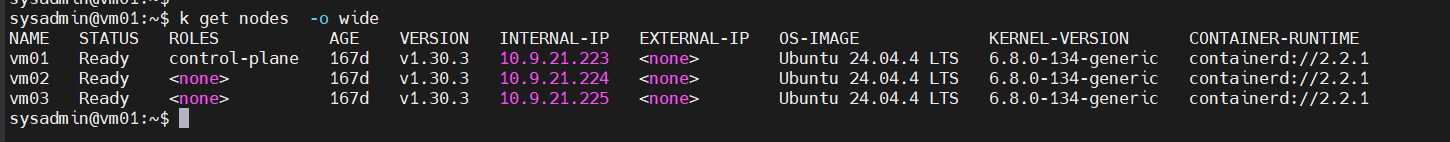
\includegraphics[width=0.9\textwidth]{image/capture_kubectl_get_nodes.png}
\caption{État des nœuds du cluster: }
\label{fig:capture-nodes}
\end{figure}

\begin{itemize}
    \item \textbf{État de Cilium:}
\end{itemize}

La figure~\ref{fig:capture-cilium-status} confirme l'état OK de Cilium, Envoy et l'opérateur, en version 1.19.1.

\begin{figure}[H]
\centering
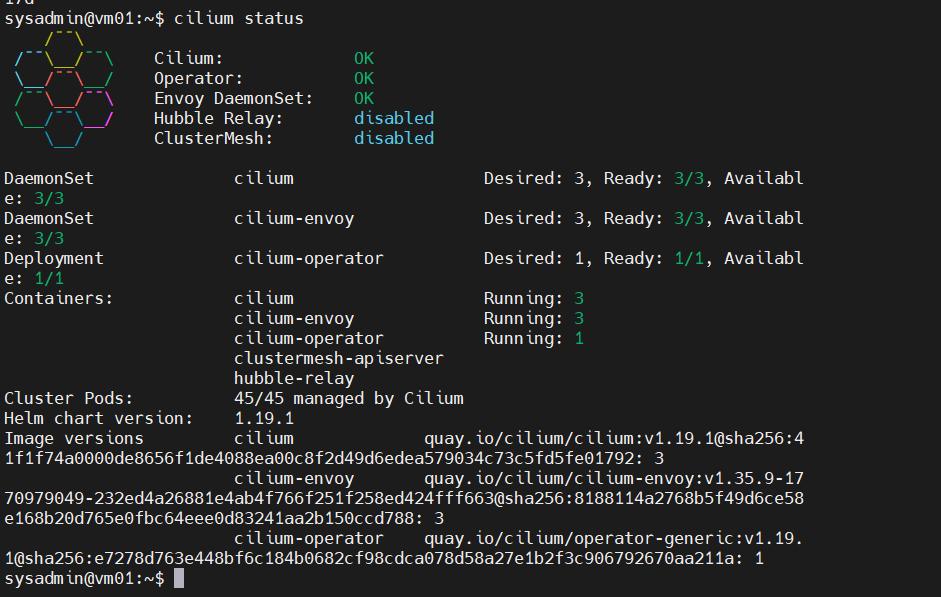
\includegraphics[width=0.85\textwidth]{image/capture_cilium_status.png}
\caption{État de Cilium}
\label{fig:capture-cilium-status}
\end{figure}

\begin{itemize}
    \item \textbf{Pods d'infrastructure réseau:}
\end{itemize}

La figure~\ref{fig:capture-pods-infra} montre les pods \texttt{kube-system} et \texttt{metallb-system} à l'état Running. On y observe une duplication non expliquée de Kourier, présent à la fois sous \texttt{net-kourier-controller} et sous une passerelle \texttt{3scale-kourier-gateway}, dans deux namespaces distincts.

\begin{figure}[H]
\centering
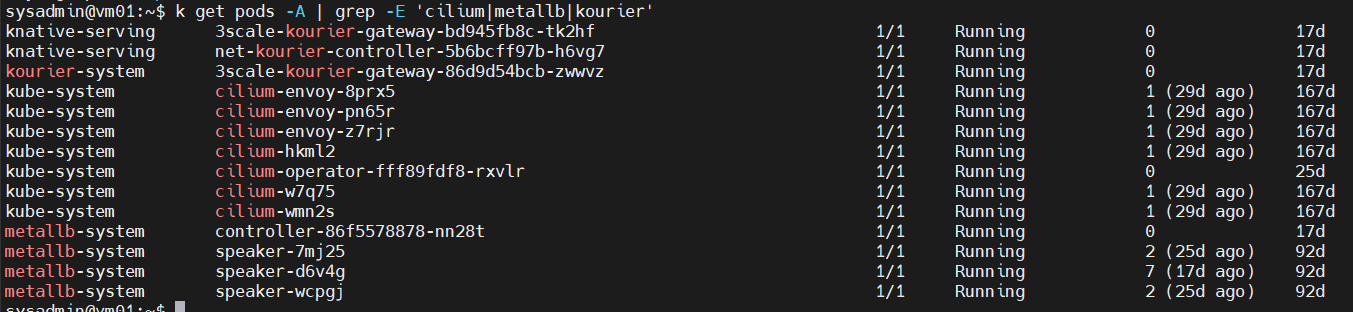
\includegraphics[width=0.9\textwidth]{image/capture_pods_infra.png}
\caption{Pods d'infrastructure réseau}
\label{fig:capture-pods-infra}
\end{figure}

\begin{itemize}
    \item \textbf{Namespaces du cluster:}
\end{itemize}

La figure~\ref{fig:capture-ns} confirme la présence du namespace \texttt{platform} et de quatre namespaces tenants.

\begin{figure}[H]
\centering
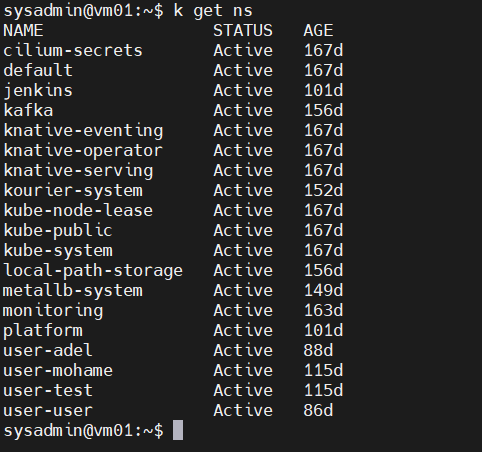
\includegraphics[width=0.85\textwidth]{image/capture_get_namespaces.png}
\caption{Namespaces du cluster}
\label{fig:capture-ns}
\end{figure}

\begin{itemize}
    \item \textbf{Politiques réseau des tenants:}
\end{itemize}

La figure~\ref{fig:capture-netpol} révèle un écart réel : seul le namespace \texttt{user-user} possède la règle \texttt{tenant-default-isolation}. Les trois autres n'en ont aucune, un point non expliqué dans le dépôt et retenu comme limite de ce sprint.

\begin{figure}[H]
\centering
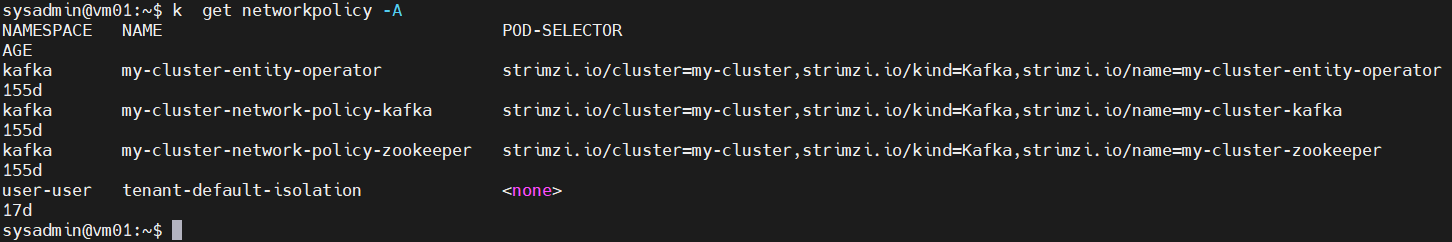
\includegraphics[width=0.85\textwidth]{image/capture_get_networkpolicy.png}
\caption{Politiques réseau des tenants}
\label{fig:capture-netpol}
\end{figure}

\section{Sprint 1 : Déploiement de Knative Serving}

\subsection{Introduction}

Le cluster livré au sprint précédent héberge des conteneurs, mais rien n'y automatise encore leur mise à l'échelle selon le trafic reçu. Knative Serving comble ce manque : son installation, son raccordement à la passerelle Kourier déjà en place et sa pilotabilité depuis le backend constituent le cœur de ce sprint. Un point conditionne toute l'intégration : il n'existe pas de client Java officiel pour les ressources Knative, ce qui impose de passer par l'API générique de Fabric8, avec les limites discutées plus loin dans ce sprint.

\subsection{Objectifs du Sprint}

\begin{itemize}
    \item Installer Knative Serving et l'intégrer à la passerelle Kourier mise en place au Sprint 0.
    \item Permettre au backend de créer une ressource Service Knative par programmation, via Fabric8.
    \item Créer automatiquement le namespace d'un tenant et sa NetworkPolicy lors de son premier déploiement.
\end{itemize}

\subsection{Sprint Backlog}

Le tableau~\ref{tab:sb-sprint1} présente le backlog détaillé du Sprint 1, obtenu en décomposant chaque User Story retenue en tâches techniques.

% \needspace garantit qu'il reste assez de place sur la page : sans cela une
% coupure peut tomber au milieu d'un groupe \multirow, dont le contenu deborde
% alors hors du cadre et laisse une cellule vide sur la page suivante.
\needspace{0.75\textheight}
{
% Le tableau deborde volontairement de 1,5 cm dans chaque marge afin de laisser
% respirer les trois colonnes ; LTleft/LTright sont les parametres propres a
% longtable (adjustwidth n'a aucun effet sur cet environnement).
% Largeur totale : 18,8 cm, soit 1 cm de blanc conserve de chaque cote de la page.
\setlength{\LTleft}{-1.5cm}
\setlength{\LTright}{-1.5cm}
\setlength{\tabcolsep}{8pt}
\renewcommand{\arraystretch}{1.9}
\begin{longtable}{|p{6.6cm}|>{\raggedright\arraybackslash}p{8.1cm}|>{\centering\arraybackslash}p{2.3cm}|}
\hline
User Story & Tâches & Estimation \\
\hline
\endfirsthead
\hline
User Story & Tâches & Estimation \\
\hline
\endhead
\endfoot
\hline

\caption{Backlog du Sprint 1}
\label{tab:sb-sprint1}
\endlastfoot

\multirow{2}{6.6cm}{
\centering
En tant qu'ADMIN, je veux que Knative Serving soit opérationnel sur le cluster.
}
&
Installer Knative Serving et l'intégrer à la passerelle Kourier mise en place au Sprint 0.
& 3 \\
\cline{2-3}

&
Vérifier qu'un Service Knative de test atteint la condition Ready et expose une URL.
& 1 \\
\hline

\multirow{3}{6.6cm}{
\centering
En tant que développeur backend, je veux pouvoir créer une ressource Knative Service par programmation.
}
&
Implémenter la création d'une ressource Service Knative via l'API générique Fabric8.
& 3 \\
\cline{2-3}

&
Vérifier que le service créé est visible via kubectl get ksvc, avec l'image demandée.
& 1 \\
\cline{2-3}

&
Observer le cycle Service vers Revision et le comportement d'autoscaling.
& 2 \\
\hline

\multirow{3}{6.6cm}{
\centering
En tant que système, je veux que l'espace de noms d'un tenant soit créé automatiquement au premier déploiement.
}
&
Implémenter la création automatique du namespace tenant et de sa NetworkPolicy au premier déploiement.
& 2 \\
\cline{2-3}

&
Vérifier l'existence du namespace et de la NetworkPolicy après un premier déploiement.
& 1 \\
\cline{2-3}

&
Observer le comportement de scale-to-zero natif de Knative.
& 2 \\
\hline

\end{longtable}
}

\subsection{Conception}

\subsubsection{Knative Serving : rôle et concepts}

Le cluster du Sprint 0 exécute des Pods et isole les tenants, mais ne gère pas encore leur nombre selon la charge. Knative Serving \cite{KnativeServingDoc} ajoute cette capacité : il fait tourner une application uniquement quand elle reçoit du trafic, et coupe les instances inutilisées.

Trois ressources le structurent : le Service (image, port, ressources, bornes de mise à l'échelle), la Revision (instantané figé de la configuration, créé à chaque modification du Service) et la Route (distribue le trafic vers une ou plusieurs révisions).

Knative ajuste le nombre de Pods d'une révision selon le trafic et peut le réduire jusqu'à zéro instance en l'absence de sollicitation (le scale-to-zero, illustré figure~\ref{fig:scale-to-zero}), avant qu'une nouvelle requête ne réactive automatiquement une instance.

\begin{figure}[H]
\begin{adjustwidth}{-1.3cm}{-1.3cm}
\centering
\begin{tikzpicture}[
  x=1cm, y=1cm,
  every node/.style={font=\normalsize},
  don/.style={draw=figBleu, line width=1pt, rounded corners, minimum width=6.0cm,
              minimum height=1.45cm, align=center, fill=figBleuFond},
  eta/.style={draw=figVert, line width=1pt, rounded corners, minimum width=6.0cm,
              minimum height=1.45cm, align=center, fill=figVertFond},
  ctl/.style={draw=figOrange, line width=1pt, dashed, rounded corners, minimum width=5.0cm,
              minimum height=1.45cm, align=center, fill=figOrangeFond},
  num/.style={circle, draw, line width=0.8pt, fill=white, inner sep=2pt, font=\small\bfseries},
  lbl/.style={font=\small},
  fl/.style={->, line width=1pt, figBleu},
  fv/.style={->, line width=1pt, figVert},
  fc/.style={->, line width=1pt, dashed, figOrange}
]

\node[eta] (s0)  at (0,0)     {État de repos : 0 Pod\\[1pt]\small la Route pointe vers l'Activator};
\node[don] (kou) at (0,-2.6)  {Kourier\\[1pt]\small passerelle d'entrée du cluster};
\node[don] (act) at (0,-5.2)  {Activator\\[1pt]\small met la requête en file d'attente};
\node[don] (pod) at (0,-9.4)  {Pod : \texttt{queue-proxy} + conteneur\\[1pt]\small l'application traite la requête};
\node[eta] (fin) at (0,-12.2) {Retour au repos\\[1pt]\small les Pods sont supprimés};

\node[ctl] (kpa)  at (9.4,-5.2)  {Autoscaler (KPA)};
\node[ctl] (rev)  at (9.4,-7.3)  {Revision $\rightarrow$ Deployment\\[1pt]\small réplicas 0 $\rightarrow$ 1};
\node[ctl] (down) at (9.4,-12.2) {Autoscaler\\[1pt]\small réplicas 1 $\rightarrow$ 0};

\draw[fl] (s0)  -- (kou);
\draw[fl] (kou) -- (act);
\draw[fc] (act.east) -- (kpa.west);
\draw[fc] (kpa) -- (rev);
\draw[fl] (rev.south) |- ([yshift=0.35cm]pod.east);
\draw[fl] (act) -- (pod);
\draw[fc] ([yshift=-0.35cm]pod.east) -- (13.0,-9.75) |- (kpa.east);
\draw[fv] (pod) -- (fin);
\draw[fc] (fin.east) -- (down.west);
\draw[fv] (down.east) -- (14.4,-12.2) |- (s0.east);

\node[lbl, anchor=east]  at (-0.3,-1.3)  {requête HTTP};
\node[lbl, anchor=south] at (4.7,-5.0)   {signale la demande};
\node[lbl, anchor=south] at (6.0,-9.3)   {le Pod démarre};
\node[lbl, anchor=east]  at (-0.3,-7.3)  {transmet la requête};
\node[lbl, anchor=north] at (7.6,-9.95)  {métriques de concurrence};
\node[lbl, anchor=east]  at (-0.3,-10.8) {inactivité prolongée};
\node[lbl, anchor=south] at (8.5,0.2)    {nouveau cycle};

\node[num] at (0,-1.3)    {1};
\node[num] at (0,-3.9)    {2};
\node[num] at (4.7,-5.2)  {3};
\node[num] at (9.4,-6.25) {4};
\node[num] at (6.0,-9.05) {5};
\node[num] at (0,-7.3)    {6};
\node[num] at (13.0,-7.5) {7};
\node[num] at (0,-10.8)   {8};
\node[num] at (4.7,-12.2) {9};

\end{tikzpicture}
\caption{Cycle complet de mise à zéro et de réveil automatique d'un service Knative}
\label{fig:scale-to-zero}
\end{adjustwidth}
\end{figure}

Ce comportement est natif à Knative et n'est pas réimplémenté par le backend. Sa preuve concrète nécessite une séquence d'observation dans le temps, non disponible à la date de rédaction.

% TODO: figures réelles à ajouter — trois captures de kubectl get pods
% -n <namespace-tenant> : (1) 1 Pod actif, (2) 0 Pod après inactivité,
% (3) 1 Pod après une nouvelle requête (preuve du scale-to-zero, S1-V05).

\subsubsection{Intégration avec Kubernetes et le backend}

Une ressource Service Knative n'est pas un objet Kubernetes natif : c'est une CRD (Custom Resource Definition), au même titre que les ressources ajoutées par Strimzi pour Kafka au Sprint 2. Elle suit le même modèle de namespace, ce qui la fait bénéficier de la NetworkPolicy default-deny du tenant concerné.

Le backend pilote cette ressource (création, lecture de statut, gestion des révisions) via la bibliothèque Fabric8 Kubernetes Client~\cite{Fabric8Doc} ; son implémentation précise est présentée au chapitre consacré au backend (Release 1). La figure~\ref{fig:backend-knative-integration} situe cette intégration dans la chaîne complète, du backend jusqu'au Pod applicatif.

\begin{figure}[H]
\begin{adjustwidth}{-1.3cm}{-1.3cm}
\centering
\begin{tikzpicture}[
  x=1cm, y=1cm,
  every node/.style={font=\normalsize},
  bk/.style={draw=figBleu, line width=1pt, rounded corners, minimum width=5.6cm,
             minimum height=1.45cm, align=center, fill=figBleuFond},
  k8s/.style={draw=figVert, line width=1pt, rounded corners, minimum width=5.6cm,
              minimum height=1.45cm, align=center, fill=figVertFond},
  crd/.style={draw=figOrange, line width=1pt, dashed, rounded corners, minimum width=5.6cm,
              minimum height=1.45cm, align=center, fill=figOrangeFond},
  lbl/.style={font=\small},
  fl/.style={->, line width=1pt, figBleu},
  fo/.style={->, line width=1pt, figOrange}
]

\node[bk]  (back) at (0,0)    {Backend Spring Boot\\[1pt]\small paramètres saisis par le client};
\node[bk]  (fab)  at (0,-2.6) {Fabric8 Kubernetes Client\\[1pt]\small construit le manifeste};
\node[k8s] (api)  at (0,-5.2) {API Kubernetes\\[1pt]\small \texttt{kube-apiserver}};

\node[crd] (svc)  at (8.8,-5.2)  {Service Knative (CRD)\\[1pt]\small dans le namespace du tenant};
\node[crd] (rev)  at (8.8,-7.8)  {Revision\\[1pt]\small instantané figé de la configuration};
\node[crd] (dep)  at (8.8,-10.4) {Deployment\\[1pt]\small géré par Knative Serving};
\node[k8s] (pod)  at (8.8,-13.0) {Pod applicatif\\[1pt]\small \texttt{queue-proxy} + conteneur client};

\draw[fl] (back) -- (fab);
\draw[fl] (fab)  -- (api);
\draw[fl] (api)  -- (svc);
\draw[fo] (svc)  -- (rev);
\draw[fo] (rev)  -- (dep);
\draw[fo] (dep)  -- (pod);

\node[lbl, anchor=east, align=right] at (-0.3,-1.3) {image, port, ressources,\\bornes de mise à l'échelle};
\node[lbl, anchor=east, align=right] at (-0.3,-3.9) {soumet la ressource\\personnalisée};
\node[lbl, anchor=south] at (4.4,-5.0)  {crée la CRD};

\node[draw=figVert, line width=1pt, rounded corners, fill=figVertFond, align=left,
      font=\small, minimum width=6.0cm] (notes) at (1.0,-13.0)
      {Hérité du namespace du tenant\\[2pt]
       $\bullet$ NetworkPolicy default-deny (Sprint 0)\\
       $\bullet$ variables d'environnement Kafka\\
       \quad injectées automatiquement (Strimzi)};
\draw[->, line width=1pt, dashed, figVert] (notes.east) -- (pod.west);

\end{tikzpicture}
\caption{Chaîne d'intégration du backend à Knative Serving}
\label{fig:backend-knative-integration}
\end{adjustwidth}
\end{figure}

Le manifeste soumis reprend les paramètres fournis par le client : image et tag Docker, port d'écoute (8080 par défaut), ressources demandées (100m CPU / 128Mi mémoire par défaut), et bornes minScale/maxScale (0 et 10 par défaut). Chaque conteneur applicatif reçoit aussi automatiquement, sans configuration du client, des variables d'environnement pointant vers le service de bootstrap Kafka opéré par Strimzi, permettant à toute application de se connecter directement au bus d'événements de la plateforme.

\subsection{Réalisation}

\subsubsection{Mise en œuvre}

Ce sprint développe et versionne la capacité du backend à créer et piloter des ressources Service Knative par programmation ; son implémentation précise est présentée au chapitre consacré au backend (Release 1). L'installation de Knative Serving elle-même, ses composants de plan de contrôle dans le namespace \texttt{knative-serving} et son intégration avec Kourier ont été réalisées directement sur l'infrastructure, selon la même approche que le socle du Sprint 0.

\begin{itemize}
    \item \textbf{Plan de contrôle de Knative Serving.}
\end{itemize}

La figure~\ref{fig:capture-knative-pods} montre les sept pods du namespace \texttt{knative-serving} à l'état Running depuis dix-huit jours : \texttt{activator}, \texttt{autoscaler} (et son variant \texttt{autoscaler-hpa}), \texttt{controller}, \texttt{webhook}, ainsi que \texttt{net-kourier-controller} et \texttt{3scale-kourier-gateway} qui assurent l'intégration avec Kourier.

\begin{figure}[H]
 \centering
    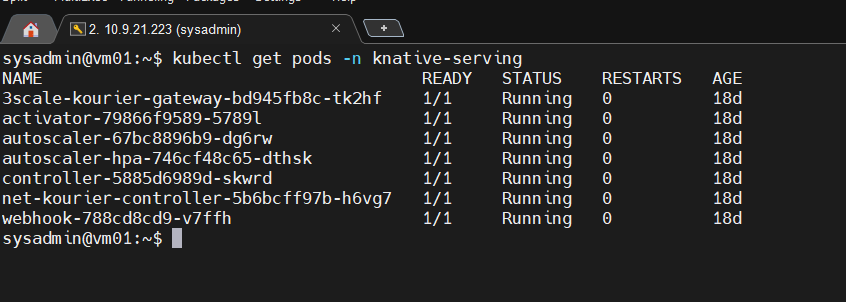
\includegraphics[width=0.92\textwidth]{image/capture_knative_pods.png}
    \caption{Composants de Knative Serving déployés sur le cluster}
    \label{fig:capture-knative-pods}
\end{figure}

\begin{itemize}
    \item \textbf{Services Knative créés par le backend dans un namespace tenant.}
\end{itemize}

La figure~\ref{fig:capture-ksvc} liste les ressources Service Knative du namespace \texttt{user-user}, créées par le backend via Fabric8, chacune avec une URL conforme à la convention \texttt{<app>.<namespace>.10.9.21.231.sslip.io} définie au Sprint 0. Deux services y apparaissent à l'état \texttt{READY: False} (motif \texttt{RevisionMissing}) : ces cas sont conservés dans la capture car ils illustrent que le suivi de statut remonte fidèlement les échecs de déploiement, la fonction attendue du \texttt{KnativeWatcher} développé au Sprint 5.

\begin{figure}[H]
 \centering
    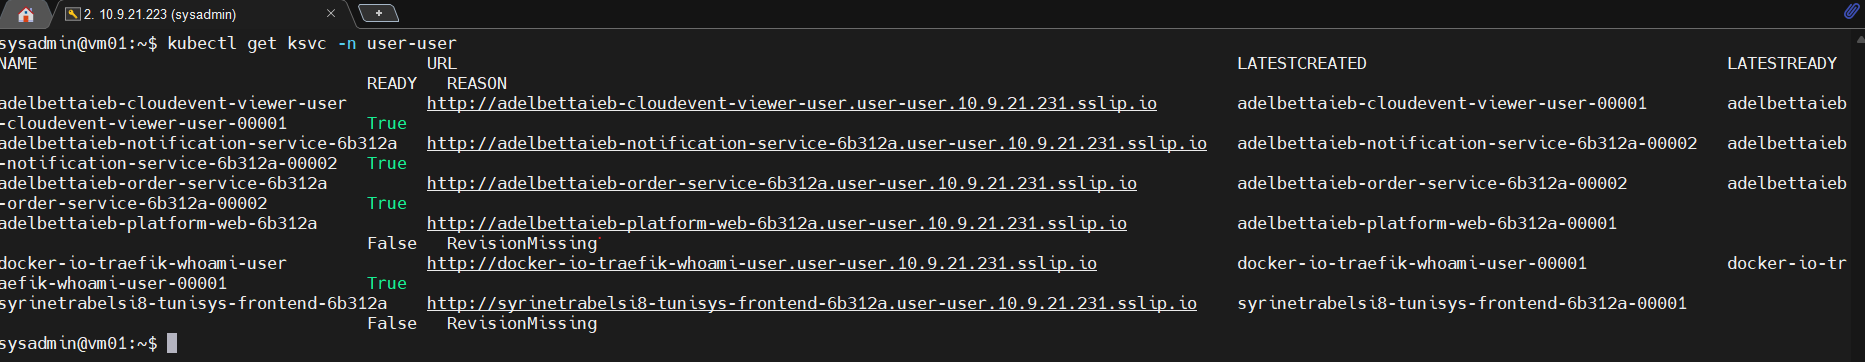
\includegraphics[width=\textwidth]{image/capture_ksvc_tenant.png}
    \caption{Services Knative d'un namespace tenant, créés par le backend}
    \label{fig:capture-ksvc}
\end{figure}

\subsubsection{Configuration et déploiement}

Le service Knative est créé avec les valeurs par défaut décrites en Conception (minScale 0, maxScale 10, port 8080, 100m CPU, 128Mi mémoire). Kourier, installé au Sprint 0, reçoit le trafic externe et le route vers la Revision active selon le nom d'hôte.

Deux limites sont à signaler : l'installation de Knative Serving elle-même n'est pas versionnée sous forme de manifestes, comme le socle du Sprint 0 ; et l'absence de client Java officiel a imposé le recours à l'API générique de Fabric8, plus verbeuse et moins sûre au niveau du typage — un choix assumé pour l'ensemble des ressources Kubernetes personnalisées du projet, par souci d'homogénéité.

À l'issue de ce sprint, le backend peut créer, par programmation, une application conteneurisée exécutée par Knative Serving, capable de monter en charge selon le trafic et de redescendre à zéro instance. Cette capacité sera exposée aux utilisateurs finaux à partir du Sprint 5.

\clearpage
\section{Sprint 2 : Mise en place de Kafka et Strimzi}

\subsection{Introduction}

La troisième brique répond à un besoin différent des deux précédentes : une plateforme serverless tire une bonne part de son intérêt de sa capacité à réagir à des événements plutôt qu'à de simples requêtes HTTP, ce qui suppose un bus de messages. Apache Kafka remplit ce rôle, déployé et administré par l'opérateur Strimzi plutôt qu'installé manuellement.

Ce sprint se limite à la gestion des topics par le backend : la publication et la consommation de messages relèvent de Knative Eventing (Sprint 3), et l'accès des clients à leurs propres topics n'arrivera qu'au Sprint 6, une fois le portail disponible.

\subsection{Objectifs du Sprint}

\begin{itemize}
    \item Déployer un cluster Apache Kafka opéré par l'opérateur Strimzi sur le cluster Kubernetes.
    \item Permettre au backend de créer, lister et supprimer des topics Kafka par programmation, via AdminClient.
\end{itemize}
\subsection{Sprint Backlog}
Le tableau~\ref{tab:sb-sprint2} présente le backlog détaillé du Sprint 2, obtenu en décomposant chaque User Story retenue en tâches techniques.

{
% Le tableau deborde volontairement de 1,5 cm dans chaque marge afin de laisser
% respirer les trois colonnes ; LTleft/LTright sont les parametres propres a
% longtable (adjustwidth n'a aucun effet sur cet environnement).
% Largeur totale : 18,8 cm, soit 1 cm de blanc conserve de chaque cote de la page.
\setlength{\LTleft}{-1.5cm}
\setlength{\LTright}{-1.5cm}
\setlength{\tabcolsep}{8pt}
\renewcommand{\arraystretch}{1.9}
\begin{longtable}{|p{6.6cm}|>{\raggedright\arraybackslash}p{8.1cm}|>{\centering\arraybackslash}p{2.3cm}|}
\hline
User Story & Tâches & Estimation \\
\hline
\endfirsthead
\hline
User Story & Tâches & Estimation \\
\hline
\endhead
\endfoot
\hline
\caption{Backlog du Sprint 2}
\label{tab:sb-sprint2}
\endlastfoot

\multirow{2}{6.6cm}{
\centering
En tant qu'ADMIN, je veux disposer d'un cluster Kafka opéré par Strimzi.
}
&
Provisionner l'opérateur Strimzi et un cluster Kafka, my-cluster, sur le cluster Kubernetes.
& 2 \\*
\cline{2-3}
&
Vérifier que le service de bootstrap my-cluster-kafka-bootstrap répond aux requêtes AdminClient.
& 1 \\
\hline

\multirow{3}{6.6cm}{
\centering
En tant que développeur backend, je veux pouvoir créer, lister et supprimer un topic Kafka par programmation.
}
&
Implémenter la création de topics via le client Kafka natif AdminClient.
& 2 \\*
\cline{2-3}
&
Implémenter le listing et la suppression de topics via AdminClient.
& 1 \\*
\hline
\cline{2-3}
&
Vérifier qu'un topic créé via AdminClient apparaît dans la liste des topics, et qu'un topic supprimé en disparaît.
& 1 \\
\hline
\end{longtable}
}

% \subsection{Sprint Backlog}

% Le tableau~\ref{tab:sb-sprint2} présente le backlog détaillé du Sprint 2, obtenu en décomposant chaque User Story retenue en tâches techniques.

% % \needspace garantit qu'il reste assez de place sur la page : sans cela une
% % coupure peut tomber au milieu d'un groupe \multirow, dont le contenu deborde
% % alors hors du cadre et laisse une cellule vide sur la page suivante.
% \needspace{0.75\textheight}
% {
% % Le tableau deborde volontairement de 1,5 cm dans chaque marge afin de laisser
% % respirer les trois colonnes ; LTleft/LTright sont les parametres propres a
% % longtable (adjustwidth n'a aucun effet sur cet environnement).
% % Largeur totale : 18,8 cm, soit 1 cm de blanc conserve de chaque cote de la page.
% \setlength{\LTleft}{-1.5cm}
% \setlength{\LTright}{-1.5cm}
% \setlength{\tabcolsep}{8pt}
% \renewcommand{\arraystretch}{1.9}
% \begin{longtable}{|p{6.6cm}|>{\raggedright\arraybackslash}p{8.1cm}|>{\centering\arraybackslash}p{2.3cm}|}
% \hline
% User Story & Tâches & Estimation \\
% \hline
% \endfirsthead
% \hline
% User Story & Tâches & Estimation \\
% \hline
% \endhead
% \endfoot
% \hline

% \caption{Backlog du Sprint 2}
% \label{tab:sb-sprint2}
% \endlastfoot

% \multirow{2}{6.6cm}{
% \centering
% En tant qu'ADMIN, je veux disposer d'un cluster Kafka opéré par Strimzi.
% }
% &
% Provisionner l'opérateur Strimzi et un cluster Kafka, my-cluster, sur le cluster Kubernetes.
% & — \\
% \cline{2-3}

% &
% Vérifier que le service de bootstrap my-cluster-kafka-bootstrap répond aux requêtes AdminClient.
% & — \\
% \hline

% \multirow{3}{6.6cm}{
% \centering
% En tant que développeur backend, je veux pouvoir créer, lister et supprimer un topic Kafka par programmation.
% }
% &
% Implémenter la création de topics via le client Kafka natif AdminClient.
% & — \\
% \cline{2-3}

% &
% Implémenter le listing et la suppression de topics via AdminClient.
% & — \\
% \cline{2-3}

% &
% Vérifier qu'un topic créé via AdminClient apparaît dans la liste des topics, et qu'un topic supprimé en disparaît.
% & — \\
% \hline

% \end{longtable}
% }

\subsection{Conception}

\subsubsection{Kafka : rôle dans la plateforme}

Knative Serving répond au besoin de faire tourner une application à la demande ; une plateforme serverless devient plus intéressante encore lorsque ce réveil peut être déclenché par un événement métier. C'est le rôle d'Apache Kafka \cite{KafkaDoc} : un bus d'événements où des composants communiquent de manière asynchrone, en publiant et consommant des messages plutôt qu'en s'appelant directement.

Un cluster Kafka repose sur des brokers, qui stockent les messages organisés en topics eux-mêmes subdivisés en partitions ; un producer publie, un consumer consomme. La figure~\ref{fig:kafka-concepts} résume ces rôles.

\begin{figure}[H]
\begin{adjustwidth}{-0.7cm}{-0.7cm}
\centering
\begin{tikzpicture}[
  x=1cm, y=1cm, every node/.style={font=\normalsize},
  act/.style={draw=figBleu, line width=1pt, rounded corners, minimum width=3.0cm,
              minimum height=1.3cm, align=center, fill=figBleuFond},
  part/.style={draw=figVert, line width=0.9pt, rounded corners, minimum width=1.6cm,
               minimum height=0.8cm, align=center, fill=white, font=\small},
  fl/.style={->, line width=1pt, figBleu}
]
\node[act] (prod) at (0,0)    {Producer};
\node[act] (cons) at (14.2,0) {Consumer};

% Cadres dessines d'abord, du plus englobant au plus interne, puis les partitions.
\draw[draw=figVert, line width=1.2pt, rounded corners, fill=figVertFond]
      (3.9,-1.8) rectangle (10.9,1.75);
\draw[draw=figVert, line width=1pt, rounded corners, fill=white]
      (4.35,-1.35) rectangle (10.45,0.65);

\node[part] (p0) at (5.4,-0.7) {partition 0};
\node[part] (p1) at (7.4,-0.7) {partition 1};
\node[part] (p2) at (9.4,-0.7) {partition 2};
\node[font=\small\bfseries, text=figVert] at (7.4,0.25) {Topic};
\node[font=\small\bfseries, text=figVert] at (7.4,1.35) {Broker Kafka};

\draw[fl] (prod.east) -- (3.9,0) node[midway, above, font=\small] {publie};
\draw[fl] (10.9,0) -- (cons.west) node[midway, above, font=\small] {consomme};
\end{tikzpicture}
\caption{Rôles fondamentaux d'un système Kafka}
\label{fig:kafka-concepts}
\end{adjustwidth}
\end{figure}

Dans la plateforme, Kafka sert de bus d'événements partagé entre applications clientes : l'une publie un événement sur un topic, une autre — potentiellement à zéro instance — est réveillée pour le traiter, via le mécanisme d'Eventing détaillé au Sprint 3.

\subsubsection{Strimzi : Kafka sur Kubernetes}

Kafka et Strimzi ne sont pas la même chose : Kafka est la plateforme de messagerie décrite ci-dessus ; Strimzi \cite{StrimziDoc} est l'opérateur Kubernetes qui l'exécute et l'administre directement sur l'infrastructure du projet.

\begin{figure}[H]
\begin{adjustwidth}{-1.0cm}{-1.0cm}
\centering
\begin{tikzpicture}[
  x=1cm, y=1cm, every node/.style={font=\normalsize},
  op/.style={draw=figOrange, line width=1pt, dashed, rounded corners, minimum width=5.6cm,
             minimum height=1.6cm, align=center, fill=figOrangeFond},
  br/.style={draw=figVert, line width=0.9pt, rounded corners, minimum width=2.4cm,
             minimum height=1.0cm, align=center, fill=white, font=\small},
  svc/.style={draw=figBleu, line width=1pt, rounded corners, minimum width=6.6cm,
              minimum height=1.5cm, align=center, fill=figBleuFond},
  note/.style={draw=black!45, dashed, line width=0.9pt, rounded corners, align=left,
               font=\small, fill=black!3}
]
\node[op] (strimzi) at (0,0)
     {Opérateur Strimzi\\[1pt]\small crée et administre le cluster Kafka};

\node[br] (b1) at (7.9,0)  {broker};
\node[br] (b2) at (10.6,0) {broker};
\node[br] (b3) at (13.3,0) {\dots};
\node[font=\small\bfseries, text=figVert] (klab) at (10.6,1.25) {Cluster Kafka \texttt{my-cluster}};

\node[svc] (boot) at (10.6,-3.4)
     {Service de bootstrap\\[1pt]\small point d'entrée interne généré par Strimzi};
\node[note] (nt) at (1.6,-3.4)
     {Écouteur interne en clair\\ni TLS ni SASL : c'est la voie\\empruntée par le backend};

\begin{scope}[on background layer]
  \node[draw=figVert, line width=1.2pt, rounded corners, inner sep=9pt, fill=figVertFond,
        fit=(b1)(b2)(b3)(klab)] (kafka) {};
\end{scope}

\draw[->, line width=1pt, figOrange, dashed] (strimzi.east) -- (kafka.west)
      node[midway, above, font=\scriptsize, fill=white, inner sep=1.5pt] {déploie et pilote};
\draw[->, line width=1pt, figVert] (kafka.south) -- (boot.north)
      node[midway, right, font=\scriptsize] {expose};

\begin{scope}[on background layer]
  \node[draw=black!50, dotted, line width=1pt, rounded corners, inner sep=15pt,
        fit=(strimzi)(kafka)(boot)(nt)] (ns) {};
\end{scope}
\node[font=\small\bfseries, text=black!65, anchor=south west]
      at ([yshift=3pt]ns.north west) {Cluster Kubernetes — namespace \texttt{kafka}};
\end{tikzpicture}
\caption{Relation entre Kubernetes, Strimzi et le cluster Kafka}
\label{fig:kafka-strimzi}
\end{adjustwidth}
\end{figure}

Le cluster Kafka de la plateforme (\texttt{my-cluster}) est opéré dans le namespace \texttt{kafka} et accessible en interne via le service de bootstrap standard généré par Strimzi. Ceci est confirmé par les variables d'environnement injectées aux applications clientes (Sprint 1). La connexion AdminClient du backend vers ce service ne configure ni TLS ni SASL. L'écouteur emprunté est donc en clair, ce qui reste acceptable tant que le trafic ne quitte pas le réseau interne du cluster.

\subsubsection{AdminClient, et non Fabric8}
\label{sec:kafka-adminclient}

Une distinction doit rester claire dans ce chapitre : Fabric8 pilote les ressources Kubernetes, Knative Serving et, au Sprint 3, Knative Eventing. Les topics Kafka, eux, ne passent pas par Fabric8 : bien que Strimzi expose une ressource personnalisée KafkaTopic, ce n'est pas le mécanisme retenu ici — créer un topic est une opération du protocole Kafka lui-même, gérée par la bibliothèque cliente AdminClient, indépendante de Kubernetes et ouverte directement vers les courtiers du cluster.

AdminClient permet de créer, lister et supprimer un topic ; son pilotage précis côté backend est présenté au chapitre qui lui est consacré (Release 1). Un nom du code peut prêter à confusion : la classe \texttt{KafkaTopic} du backend n'est pas la ressource Strimzi du même nom, mais une entité de persistance propre qui conserve en base les métadonnées de chaque topic client. La figure~\ref{fig:backend-kafka-adminclient} illustre la chaîne d'intégration réelle.

\begin{figure}[H]
\begin{adjustwidth}{-1.4cm}{-1.4cm}
\centering
\begin{tikzpicture}[
  x=1cm, y=1cm, every node/.style={font=\normalsize},
  acteur/.style={draw=black!65, line width=1.1pt, rounded corners, minimum width=4.4cm,
                 minimum height=1.3cm, align=center, fill=black!6},
  comp/.style={draw=figBleu, line width=1pt, rounded corners, minimum width=6.6cm,
               minimum height=1.4cm, align=center, fill=figBleuFond, font=\small},
  kfk/.style={draw=figOrange, line width=1pt, rounded corners, minimum width=6.6cm,
              minimum height=1.4cm, align=center, fill=figOrangeFond, font=\small},
  db/.style={draw=figVert, line width=1pt, rounded corners, minimum width=4.2cm,
             minimum height=1.4cm, align=center, fill=figVertFond, font=\small},
  hors/.style={draw=black!40, dotted, line width=1pt, rounded corners, align=left,
               font=\small, fill=black!3, text=black!60},
  zone/.style={rounded corners, inner sep=13pt, line width=1.1pt},
  num/.style={circle, draw, line width=0.8pt, fill=white, inner sep=2pt, font=\small\bfseries},
  et/.style={font=\small, align=left}
]

% ---------------- acteur ----------------
\node[acteur] (act) at (0,2.6) {CLIENT\_ADMIN\\[1pt]\footnotesize depuis le portail};

% ---------------- zone backend ----------------
\node[comp] (ctrl) at (0,-0.6)  {KafkaController / KafkaService\\\footnotesize vérifie les droits, résout le propriétaire};
\node[comp] (adm)  at (0,-3.1)  {AdminClient\\\footnotesize bibliothèque cliente du protocole Kafka};
\node[comp] (ent)  at (9.4,-0.6){entité \texttt{KafkaTopic} (JPA)\\\footnotesize métadonnées du topic};

\begin{scope}[on background layer]
  \node[zone, draw=figBleu, dashed, fill=figBleu!4, fit=(ctrl)(adm)(ent)] (zbk) {};
\end{scope}
\node[font=\small\bfseries, text=figBleu, anchor=south west, fill=white, inner sep=2pt] at ([yshift=3pt]zbk.north west)
     {Backend Spring Boot — namespace \texttt{platform}};

% ---------------- zone cluster kafka ----------------
\node[kfk] (boot) at (0,-7.9) {Service de bootstrap\\\footnotesize point d'entrée interne du cluster};
\node[kfk] (brok) at (0,-10.4) {Courtiers\\\footnotesize le topic est créé avec ses partitions};

\begin{scope}[on background layer]
  \node[zone, draw=figOrange, dashed, fill=figOrange!4, fit=(boot)(brok)] (zkf) {};
\end{scope}
\node[font=\small\bfseries, text=figOrange, anchor=south west, fill=white, inner sep=2pt] at ([yshift=3pt]zkf.north west)
     {Cluster Kafka \texttt{my-cluster} — namespace \texttt{kafka}};

% ---------------- base de donnees ----------------
\node[db] (pg) at (9.4,-3.1) {PostgreSQL};

% ---------------- fleches ----------------
\draw[->, line width=1pt, black!65] (act) -- (ctrl);
\draw[->, line width=1pt, figBleu]  (ctrl) -- (adm);
\draw[->, line width=1pt, figOrange](adm.south) -- (boot.north);
\draw[->, line width=1pt, figOrange](boot) -- (brok);
\draw[->, line width=1pt, figVert]  (ctrl.east) -- (ent.west);
\draw[->, line width=1pt, figVert]  (ent) -- (pg);

% ---------------- numeros et etapes ----------------
\node[num] at (0,1.45)  {1};
\node[num] at (0,-1.85) {2};
\node[num] at (0,-5.5)  {3};
\node[num] at (0,-9.15) {4};
\node[num] at (4.7,-0.6){5};
\node[num] at (9.4,-1.85){6};

\node[et, anchor=west] at (0.35,1.45)  {demande la création d'un topic};
\node[et, anchor=west] at (0.35,-1.85) {délègue au client Kafka};
\node[et, anchor=west, text=figOrange] at (0.35,-5.5)
     {ouvre une connexion vers les courtiers\\\footnotesize sans passer par l'API Kubernetes};
\node[et, anchor=west, text=figOrange] at (0.35,-9.15) {exécute \texttt{createTopics}};
\node[et, anchor=south] at (4.7,-0.35) {\footnotesize enregistre};
\node[et, anchor=west, text=figVert] at (9.75,-1.85) {\footnotesize persiste};

% ---------------- ce qui n'intervient pas ----------------
\node[hors] (nk) at (10.6,-9.15)
     {API Kubernetes\\
      n'intervient pas dans ce flux.\\
      Elle sert à Fabric8 pour Knative\\
      et l'Eventing. La ressource Strimzi\\
      \texttt{KafkaTopic} (CRD) n'est pas\\
      utilisée dans ce projet.};

\end{tikzpicture}
\caption{Chaîne d'intégration du backend au cluster Kafka via AdminClient}
\label{fig:backend-kafka-adminclient}
\end{adjustwidth}
\end{figure}

\subsection{Réalisation}

\subsubsection{Mise en œuvre}

Ce sprint livre le cluster Kafka opéré par Strimzi, ainsi que la capacité du backend à créer et gérer des topics par programmation ; son implémentation précise (persistance, contrôles d'accès) est présentée au chapitre consacré au backend (Release 1). Son exposition aux clients via une interface graphique ne sera livrée qu'au Sprint 6.

\begin{itemize}
    \item \textbf{Composants du cluster Kafka.}
\end{itemize}

La figure~\ref{fig:capture-kafka-pods} montre les pods du namespace \texttt{kafka} (opérateur \texttt{strimzi-cluster-operator}, courtier \texttt{my-cluster-kafka-0}, instance ZooKeeper et entity-operator), tous à l'état Running depuis dix-huit jours.

\begin{figure}[H]
 \centering
    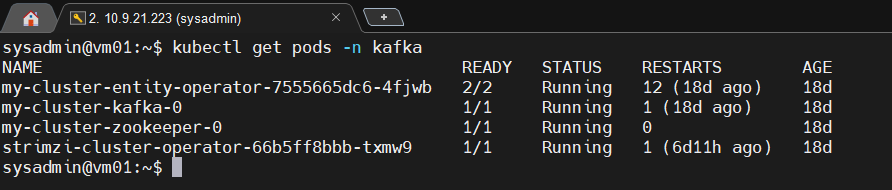
\includegraphics[width=0.92\textwidth]{image/capture_kafka_pods.png}
    \caption{Composants du cluster Kafka opéré par Strimzi}
    \label{fig:capture-kafka-pods}
\end{figure}

\begin{itemize}
    \item \textbf{Ressource Kafka gérée par l'opérateur.}
\end{itemize}

La figure~\ref{fig:capture-kafka-cluster} affiche la ressource personnalisée \texttt{Kafka} réconciliée par Strimzi, avec un courtier et une instance ZooKeeper désirés, à l'état \texttt{READY: True}, en mode ZooKeeper plutôt que KRaft.

\begin{figure}[H]
 \centering
    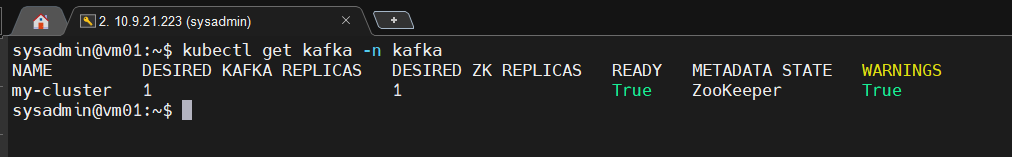
\includegraphics[width=0.92\textwidth]{image/capture_kafka_cluster.png}
    \caption{Ressource personnalisée \texttt{Kafka} réconciliée par l'opérateur Strimzi}
    \label{fig:capture-kafka-cluster}
\end{figure}

\begin{itemize}
    \item \textbf{Points d'accès réseau du cluster Kafka.}
\end{itemize}

La figure~\ref{fig:capture-kafka-svc} liste les services exposés dans le namespace \texttt{kafka}. Le backend contacte en interne le service \texttt{my-cluster-kafka-bootstrap} (\texttt{ClusterIP}) sur le port 9092.

\begin{figure}[H]
 \centering
    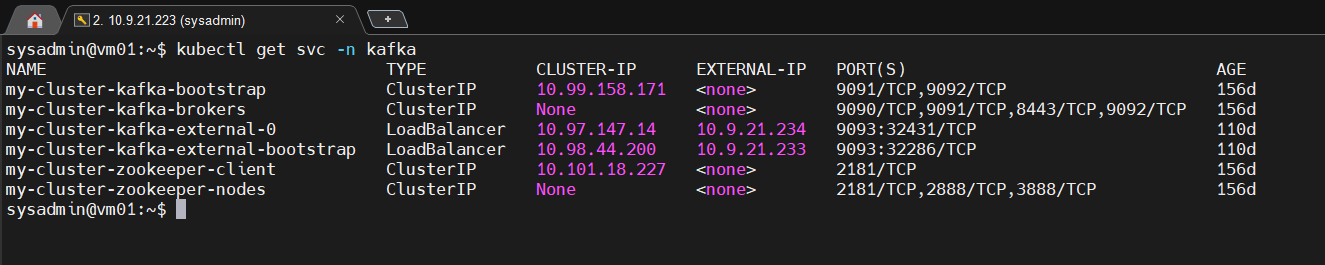
\includegraphics[width=\textwidth]{image/capture_kafka_svc.png}
    \caption{Services exposés par le cluster Kafka dans le namespace \texttt{kafka}}
    \label{fig:capture-kafka-svc}
\end{figure}

\subsubsection{Configuration et déploiement}

Le cluster Kafka \texttt{my-cluster} est provisionné dans le namespace \texttt{kafka} ; le backend s'y connecte via le service de bootstrap, sans authentification, sur le réseau interne. Comme les autres briques de ce socle, son installation n'est pas versionnée dans le dépôt, où seule la gestion applicative des topics via AdminClient figure.

L'inspection de la ressource \texttt{Kafka} précise le dimensionnement retenu : Strimzi 0.45.0, un courtier et une instance ZooKeeper, chacun adossé à un volume persistant de 1 Gio (\texttt{local-path}) — un dimensionnement d'environnement de développement, suffisant pour valider la chaîne fonctionnelle de cette release, qu'une exploitation réelle demanderait de renforcer (plusieurs courtiers, stockage répliqué).

Deux points d'accès \texttt{LoadBalancer} complètent le service de bootstrap interne, sur le port 9093, pour permettre la connexion d'outils de développement externes ; leur exposition constitue un risque assumé dans le périmètre de développement de ce projet.

Au terme de cette release, le cluster dispose des trois briques d'infrastructure fondamentales de la plateforme : orchestration Kubernetes isolée par tenant, exécution serverless via Knative Serving, et messagerie événementielle via Kafka et Strimzi. Le backend peut créer, lister et supprimer des topics Kafka par programmation ; cette capacité sera exposée aux clients via l'interface graphique à partir du Sprint 6.

\section{Conclusion}

La Release 0 a permis de construire, de manière incrémentale et validée à chaque étape, le socle cloud native de la plateforme : cluster Kubernetes isolé par tenant (Sprint 0), exécution serverless via Knative Serving (Sprint 1), bus d'événements Kafka opéré par Strimzi (Sprint 2). Cette approche progressive, conforme à la méthodologie Scrum retenue, a permis de valider chaque brique et d'en documenter honnêtement les mécanismes d'intégration réels, avant d'y adosser la logique métier présentée au chapitre suivant.


\chapter{Release 1 : Cœur applicatif}

\section{Introduction}

La Release 0 a livré le socle technique de la plateforme : cluster Kubernetes isolé par tenant, exécution serverless via Knative Serving, bus d'événements Kafka opéré par Strimzi. La Release 1, objet de ce chapitre, organise le cœur applicatif de la plateforme par domaine de gestion fonctionnelle, plutôt que par brique technique livrée : chaque sprint regroupe l'ensemble des fonctionnalités d'un même domaine, tous les acteurs concernés confondus, et livre conjointement la brique backend et l'écran du portail qui l'expose.

Elle regroupe quatre sprints : le Sprint 3, qui met en place les accès et l'identité des utilisateurs, préalable à tout le reste ; le Sprint 4, qui livre le cycle de vie complet d'une application ; le Sprint 5, qui relie Kafka et Knative Eventing en un service de messagerie événementielle complet, de la brique backend jusqu'aux écrans du portail ; et le Sprint 6, qui livre l'observabilité applicative (journaux, métriques).

\clearpage
\section{Sprint 3 : Gestion des utilisateurs et des accès}

\subsection{Introduction}

Ce sprint met en place l'identité et le contrôle d'accès de la plateforme : création de compte, connexion, gestion du profil, gestion des rôles côté ADMIN, gestion d'équipe côté CLIENT\_ADMIN. Aucune autre fonctionnalité de la plateforme ne peut être protégée par rôle ou par permission tant que ce socle n'existe pas ; ce sprint précède donc logiquement tous les suivants.

L'authentification passe entièrement par Keycloak. Le backend ne gère ni mot de passe ni session : c'est un serveur de ressources OAuth2, qui valide les jetons émis par Keycloak et en extrait le rôle applicatif.

\subsection{Sprint Backlog}

Le tableau~\ref{tab:sb-sprint3} présente le backlog détaillé du Sprint 3, obtenu en décomposant chaque User Story retenue en tâches techniques.

\needspace{0.9\textheight}
{
\setlength{\LTleft}{-1.5cm}
\setlength{\LTright}{-1.5cm}
\setlength{\tabcolsep}{8pt}
\renewcommand{\arraystretch}{1.9}
\begin{longtable}{|p{6.6cm}|>{\raggedright\arraybackslash}p{8.1cm}|>{\centering\arraybackslash}p{2.3cm}|}
\hline
User Story & Tâches & Estimation \\
\hline
\endfirsthead
\hline
User Story & Tâches & Estimation \\
\hline
\endhead
\hline
\endfoot

\caption{Backlog du Sprint 3}
\label{tab:sb-sprint3}
\endlastfoot

\multirow{3}{6.6cm}{\centering En tant que CLIENT\_ADMIN, je veux créer un compte afin d'accéder à la plateforme et gérer mon équipe.}
& Créer le compte dans Keycloak. & 1 \\ \cline{2-3}
& Synchroniser l'utilisateur avec la plateforme. & 1 \\ \cline{2-3}
& Tester la création du compte. & 1 \\ \hline

\multirow{3}{6.6cm}{\centering En tant qu'ADMIN, CLIENT\_ADMIN ou MEMBER, je veux me connecter afin d'accéder à la plateforme.}
& Intégrer Keycloak au mécanisme d'authentification. & 1 \\ \cline{2-3}
& Développer l'interface de connexion. & 1 \\ \cline{2-3}
& Vérifier l'authentification et le rôle de l'utilisateur. & 1 \\ \hline

\multirow{3}{6.6cm}{\centering En tant qu'ADMIN, CLIENT\_ADMIN ou MEMBER, je veux consulter et modifier mon profil.}
& Développer la consultation du profil. & 1 \\ \cline{2-3}
& Développer la modification du profil. & 1 \\ \cline{2-3}
& Tester la mise à jour du profil. & 1 \\ \hline

\multirow{4}{6.6cm}{\centering En tant qu'ADMIN, je veux gérer les utilisateurs de la plateforme.}
& Développer la liste des utilisateurs. & 1 \\ \cline{2-3}
& Développer la modification du rôle d'un utilisateur. & 1 \\ \cline{2-3}
& Développer l'interface d'administration (admin-console). & 1 \\ \cline{2-3}
& Tester la gestion des utilisateurs. & 1 \\ \hline

\multirow{5}{6.6cm}{\centering En tant que CLIENT\_ADMIN, je veux gérer mon équipe.}
& Développer l'ajout d'un membre. & 1 \\ \cline{2-3}
& Développer la liste des membres. & 1 \\ \cline{2-3}
& Développer la modification des permissions. & 1 \\ \cline{2-3}
& Développer la suppression d'un membre. & 1 \\ \cline{2-3}
& Développer l'interface de gestion de l'équipe. & 1 \\ \hline

\end{longtable}
}

\subsection{Diagramme de cas d'utilisation du Sprint 3}

Le diagramme réunit les quatre acteurs de ce sprint (Visiteur, MEMBER, CLIENT\_ADMIN, ADMIN, les trois derniers généralisés sous un acteur commun « Utilisateur authentifié » pour les cas d'utilisation qu'ils partagent) et l'ensemble des dix fonctionnalités du sprint.

\begin{figure}[H]
 \centering
    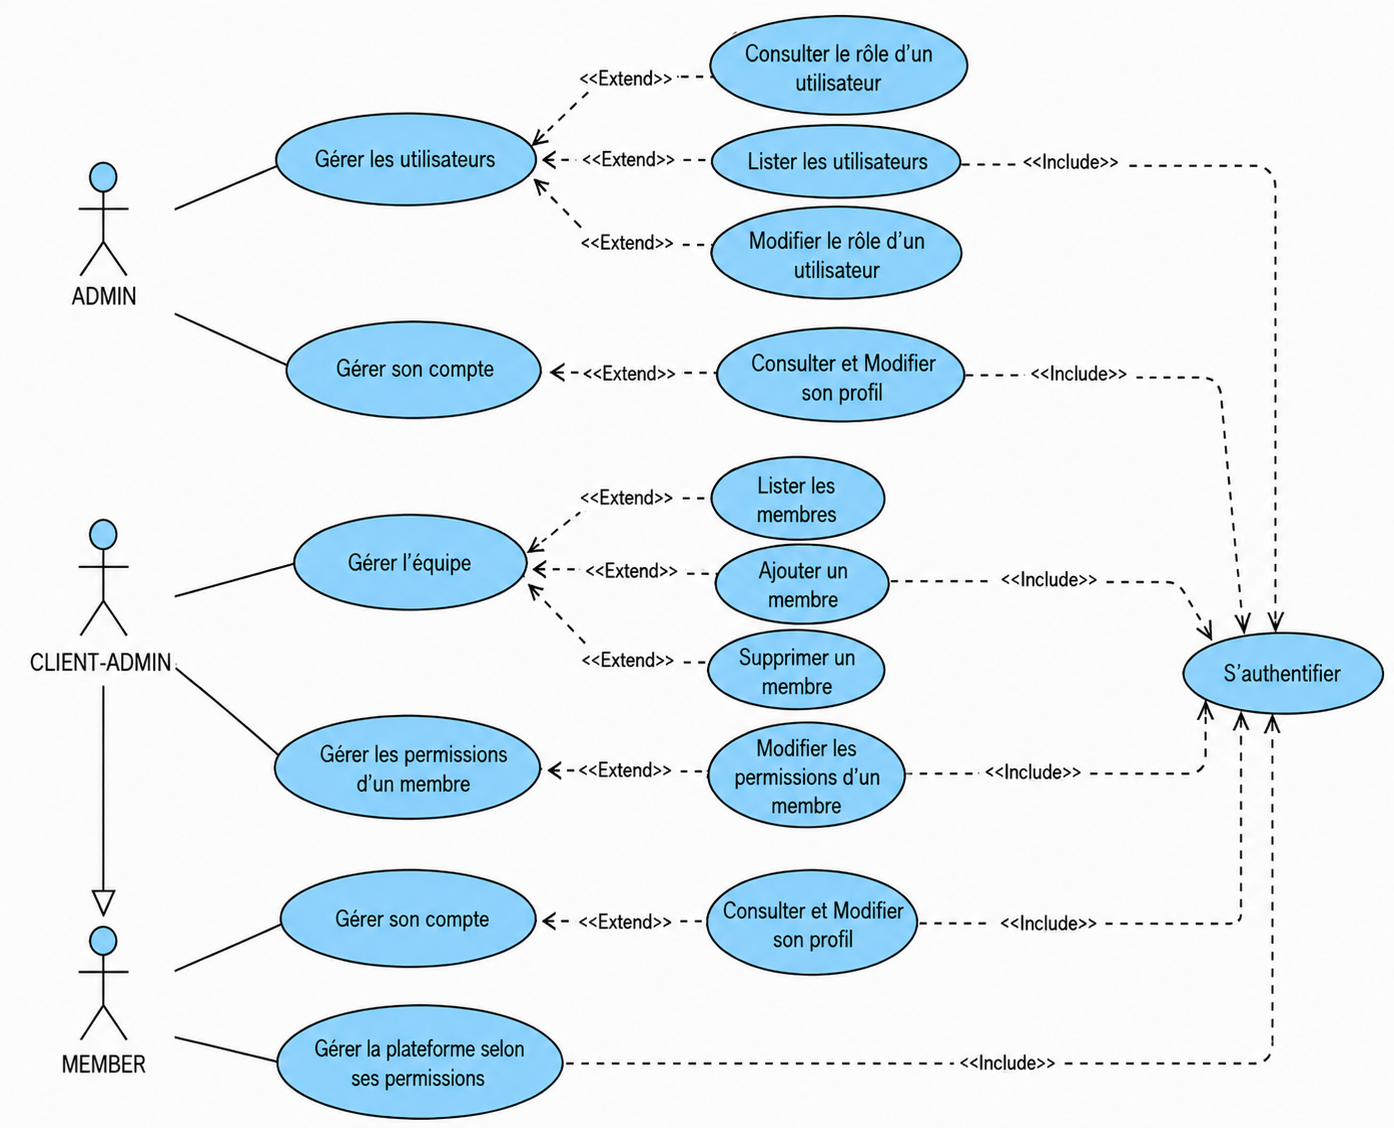
\includegraphics[width=0.85\textwidth]{image/uc-sprint3.png}
    \caption{Diagramme de cas d'utilisation du Sprint 3 — Gestion des utilisateurs et des accès}
    \label{fig:uc-sprint3}
\end{figure}

\subsection{Services Web}

\needspace{5cm}
\begin{longtable}{|p{6cm}|p{9.3cm}|}
\hline
Service Web & Description \\
\hline
\endfirsthead
\hline
Service Web & Description \\
\hline
\endhead
\hline
\endfoot
\endlastfoot
\texttt{POST /api/auth/register} & Créer un compte. \\ \hline
Connexion (Keycloak, OIDC) & Échange des identifiants contre un jeton, hors API du backend. \\ \hline
\texttt{GET /api/users/me} & Consulter son profil. \\ \hline
\texttt{PATCH /api/users/me} & Modifier son profil. \\ \hline
\texttt{GET /api/users} & Lister les utilisateurs (ADMIN). \\ \hline
\texttt{PATCH /api/users/\{id\}/role} & Modifier le rôle d'un utilisateur (ADMIN). \\ \hline
\texttt{GET /api/team/members} & Lister les membres de son équipe. \\ \hline
\texttt{POST /api/team/members} & Ajouter un membre. \\ \hline
\texttt{PUT /api/team/members/\{id\}/permissions} & Modifier les permissions d'un membre. \\ \hline
\texttt{DELETE /api/team/members/\{id\}} & Supprimer un membre. \\ \hline
\end{longtable}

\subsection{Conception}

Une fonctionnalité est détaillée : l'ajout d'un membre, la plus distinctive sur le plan métier de ce sprint, puisqu'elle ne suit pas un flux d'invitation classique.

\subsubsection{Cas d'utilisation : « Ajouter un membre »}

\subsubsection*{Description textuelle}

\needspace{8cm}
\renewcommand{\arraystretch}{1.5}
\begin{longtable}{|p{4cm}|p{11cm}|}
\hline
Nom & Ajouter un membre à son équipe \\
\hline
Acteur & CLIENT\_ADMIN \\
\hline
Pré-condition & Le CLIENT\_ADMIN est authentifié \\
\hline
Scénario nominal & 1. Le CLIENT\_ADMIN saisit le nom d'utilisateur, l'e-mail et le mot de passe du futur membre. \newline
2. Le backend crée le compte dans Keycloak, avec ce mot de passe marqué comme permanent. \newline
3. Le backend crée l'utilisateur local correspondant, rôle MEMBER, rattaché au compte du CLIENT\_ADMIN. \\
\hline
Post-condition & Le membre peut se connecter immédiatement avec les identifiants qui lui ont été transmis en dehors du système. \\
\hline
\caption{Description textuelle du cas d'utilisation « Ajouter un membre »}
\label{tab:uc-add-member}
\end{longtable}

Il ne s'agit pas d'un flux d'invitation par e-mail : le CLIENT\_ADMIN choisit lui-même les identifiants du membre, qu'il lui communique par un canal de son choix.

\subsubsection*{Diagramme de séquence}

\begin{figure}[H]
 \centering
    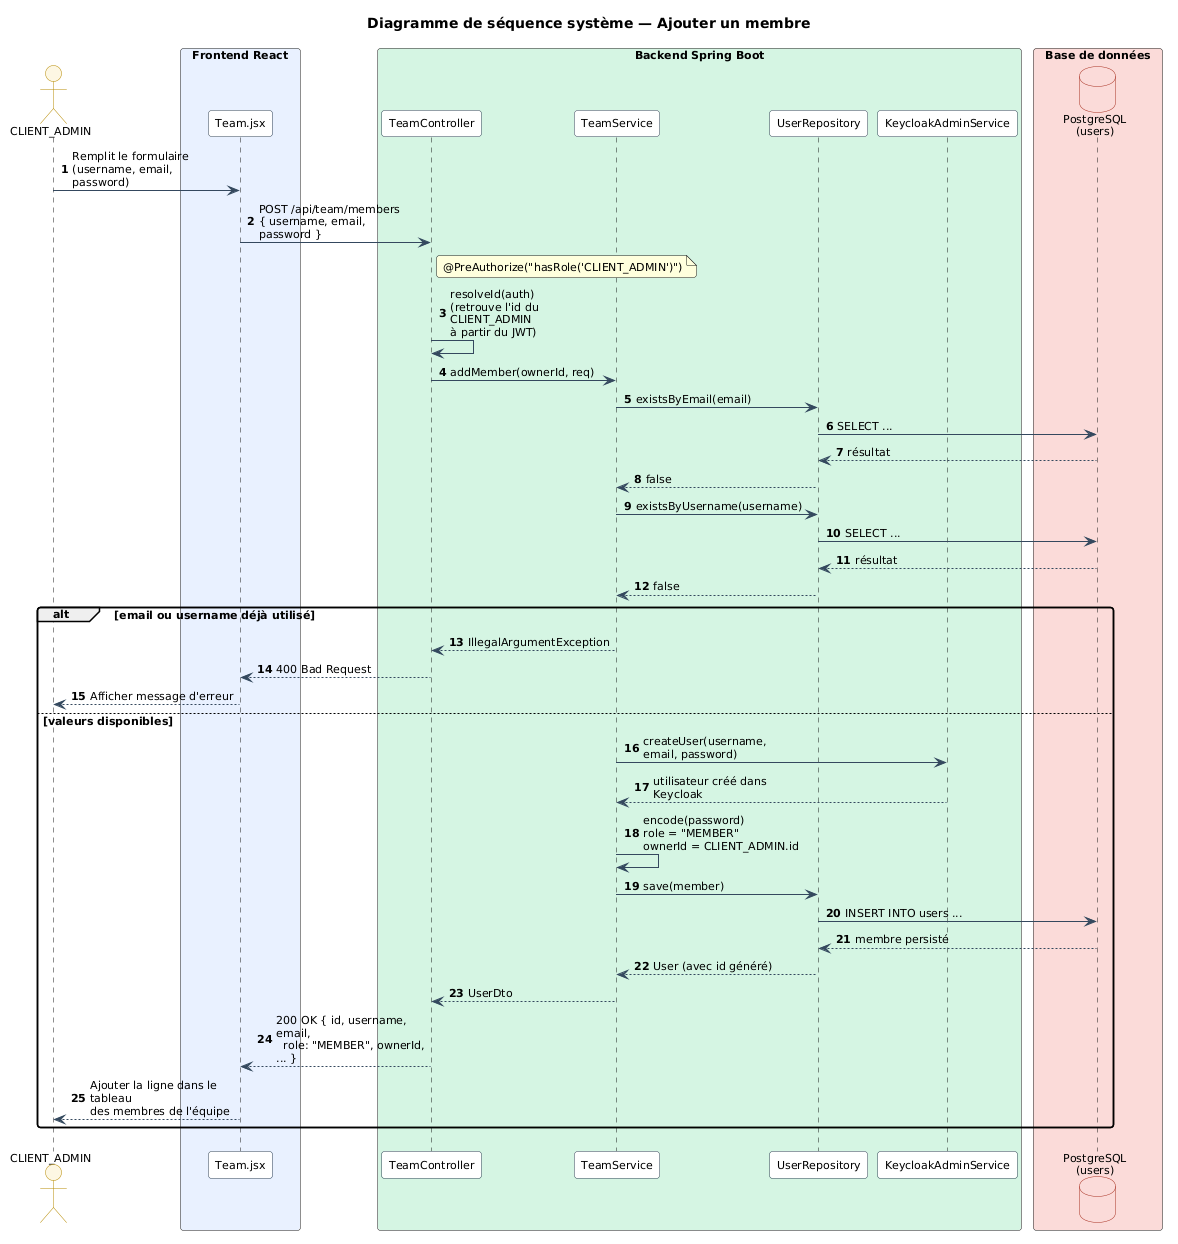
\includegraphics[width=0.7\textwidth]{image/seq-addmember.png}
    \caption{Diagramme de séquence — Ajouter un membre}
    \label{fig:seq-addmember}
\end{figure}

\subsection{Réalisation du Sprint 3}

Fonctionnalité : Créer un compte. Un visiteur peut créer un compte depuis le portail. Le rôle attribué par défaut est MEMBER, sans compte propriétaire : un tel compte ne peut effectuer aucune action tant qu'un ADMIN ne lui attribue pas un rôle actif.

Fonctionnalité : Se connecter. L'utilisateur se connecte avec son compte, quel que soit son rôle, depuis la même interface.

\begin{figure}[H]
 \centering
    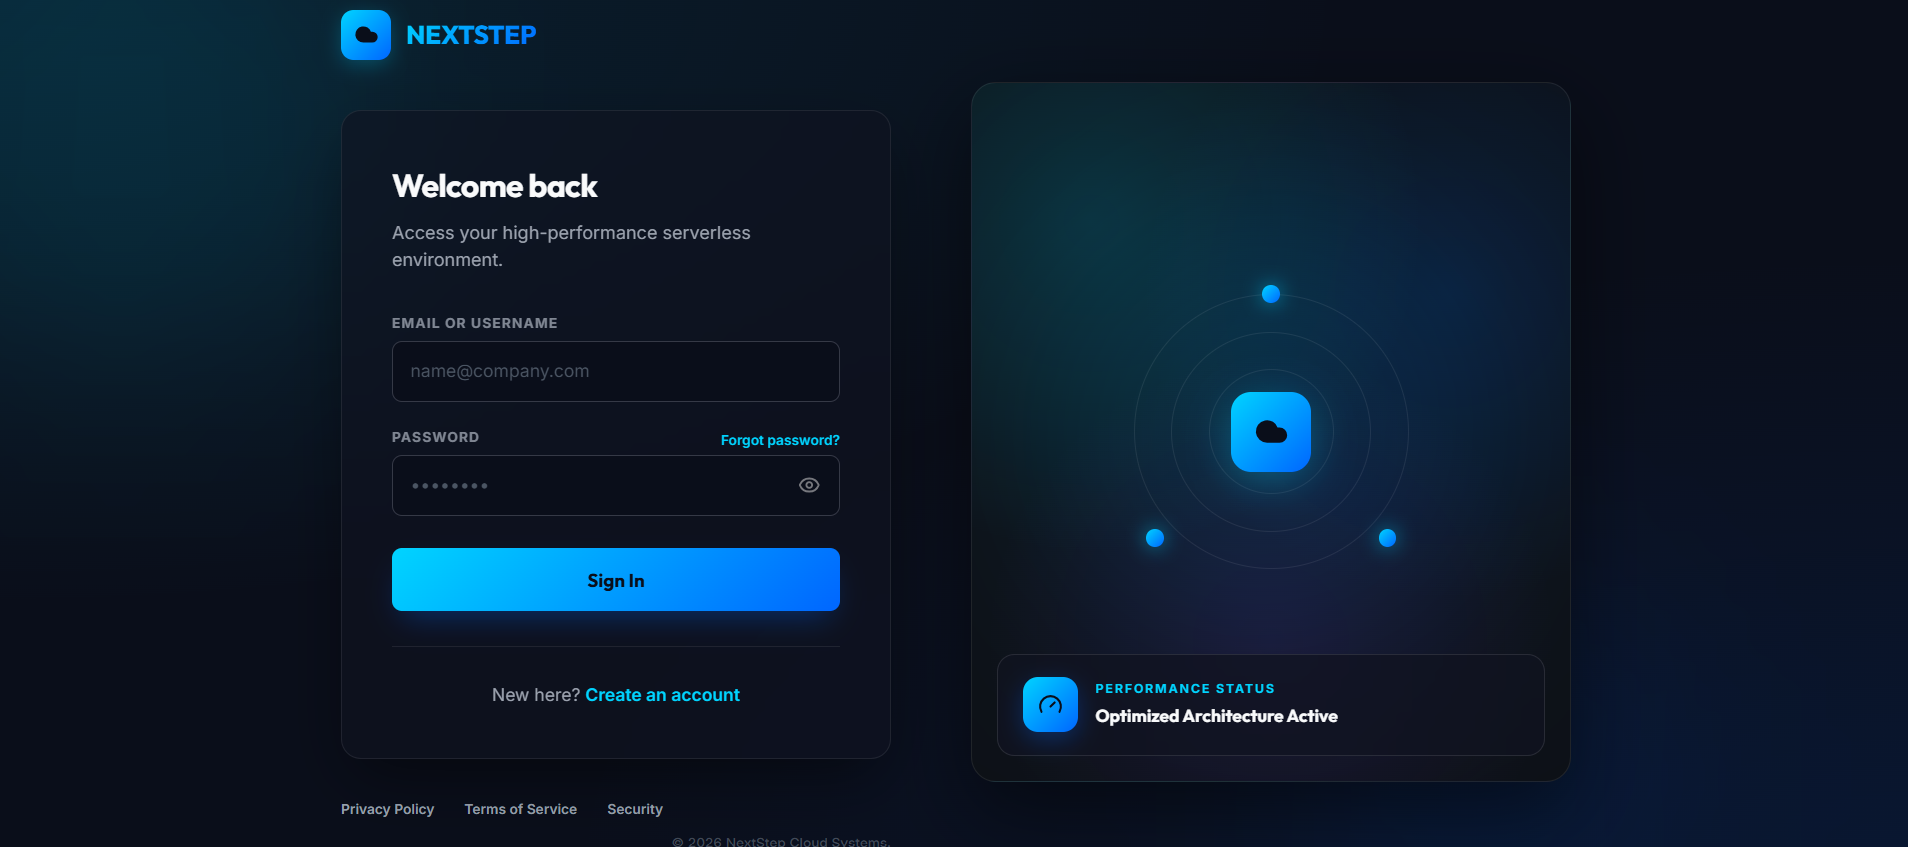
\includegraphics[width=\textwidth]{image/capture-login.png}
    \caption{Interface de connexion}
    \label{fig:capture-login}
\end{figure}

Fonctionnalité : Consulter et modifier son profil. Chaque utilisateur consulte et met à jour ses informations de profil depuis les paramètres de son compte.

\EmplacementFigure{13cm}{8cm}{Interface de gestion du profil}{fig:capture-profile}

Fonctionnalité : Gérer les utilisateurs (ADMIN). L'ADMIN consulte la liste des utilisateurs de la plateforme et modifie leur rôle depuis la console d'administration.

Fonctionnalité : Gérer son équipe (CLIENT\_ADMIN). Le CLIENT\_ADMIN consulte la liste des membres de son équipe, en ajoute, en supprime, et modifie leurs permissions individuellement.

\begin{figure}[H]
 \centering
    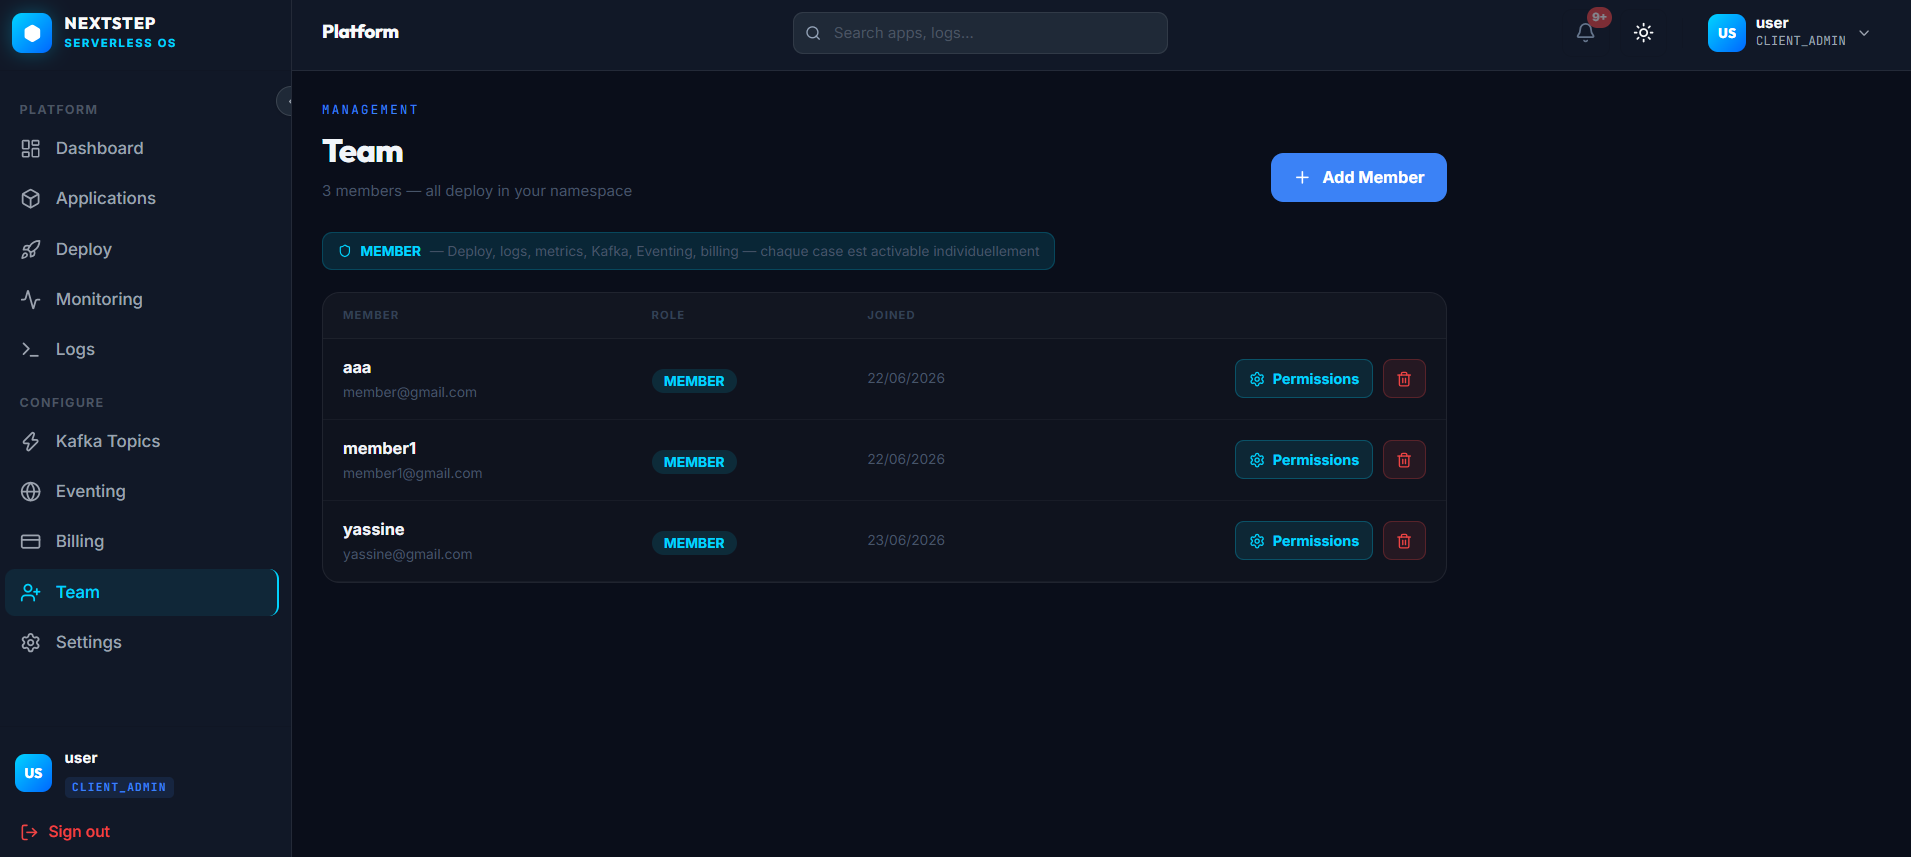
\includegraphics[width=\textwidth]{image/capture-team.png}
    \caption{Interface de gestion de l'équipe}
    \label{fig:capture-team}
\end{figure}

\subsection{Conclusion}

Ce sprint livre l'identité et le contrôle d'accès de la plateforme : connexion commune aux trois rôles, gestion des utilisateurs côté ADMIN, gestion d'équipe côté CLIENT\_ADMIN. Toutes les fonctionnalités développées dans les sprints suivants s'appuient sur ce socle de rôles et de permissions.

\clearpage
\section{Sprint 4 : Gestion des applications}

\subsection{Introduction}

Ce sprint livre le cycle de vie complet d'une application cliente : déploiement, consultation, mise à jour, suppression, historique des révisions et retour à une version antérieure, ainsi que les actions de suspension et de suppression forcée réservées à l'ADMIN. C'est la première fonctionnalité complète et accessible de bout en bout depuis le portail, appuyée sur les accès mis en place au Sprint 3 et sur Knative Serving (Release 0).

\subsection{Sprint Backlog}

Le tableau~\ref{tab:sb-sprint4} présente le backlog détaillé du Sprint 4, obtenu en décomposant chaque User Story retenue en tâches techniques.

\needspace{0.9\textheight}
{
\setlength{\LTleft}{-1.5cm}
\setlength{\LTright}{-1.5cm}
\setlength{\tabcolsep}{8pt}
\renewcommand{\arraystretch}{1.9}
\begin{longtable}{|p{6.6cm}|>{\raggedright\arraybackslash}p{8.1cm}|>{\centering\arraybackslash}p{2.3cm}|}
\hline
User Story & Tâches & Estimation \\
\hline
\endfirsthead
\hline
User Story & Tâches & Estimation \\
\hline
\endhead
\hline
\endfoot

\caption{Backlog du Sprint 4}
\label{tab:sb-sprint4}
\endlastfoot

\multirow{4}{6.6cm}{\centering En tant que CLIENT\_ADMIN ou MEMBER (avec permission DEPLOY\_APP), je veux déployer une application à partir d'une image Docker afin de la mettre en service.}
& Développer l'API de déploiement. & 1 \\* \cline{2-3}
& Développer le formulaire de déploiement du portail. & 1 \\* \cline{2-3}
& Intégrer la création de la ressource Knative correspondante. & 1 \\* \cline{2-3}
& Tester le déploiement d'une application. & 1 \\ \hline

\multirow{3}{6.6cm}{\centering En tant que CLIENT\_ADMIN ou MEMBER, je veux consulter mes applications et leur statut afin de suivre leur état.}
& Développer la liste des applications. & 1 \\* \cline{2-3}
& Développer la page de détail d'une application. & 1 \\* \cline{2-3}
& Synchroniser le statut en temps réel depuis Kubernetes. & 1 \\ \hline

\multirow{3}{6.6cm}{\centering En tant que CLIENT\_ADMIN ou MEMBER (avec permission DEPLOY\_APP/DELETE\_APP), je veux modifier, redéployer ou supprimer une application afin d'en gérer le cycle de vie.}
& Développer la mise à jour et le redéploiement. & 1 \\* \cline{2-3}
& Développer la suppression d'une application. & 1 \\* \cline{2-3}
& Tester la suppression et la mise à jour. & 1 \\ \hline

\multirow{3}{6.6cm}{\centering En tant que CLIENT\_ADMIN ou MEMBER (avec permission DEPLOY\_APP), je veux consulter l'historique des révisions et revenir à une version antérieure afin de corriger un déploiement défectueux.}
& Développer la liste des révisions. & 1 \\* \cline{2-3}
& Développer le retour à une révision antérieure. & 1 \\* \cline{2-3}
& Tester ce retour en arrière. & 1 \\ \hline

\multirow{3}{6.6cm}{\centering En tant qu'ADMIN, je veux suspendre, restaurer ou supprimer de force une application afin de gérer les abus ou incidents.}
& Développer la suspension et la restauration d'une application. & 1 \\* \cline{2-3}
& Développer la suppression forcée. & 1 \\* \cline{2-3}
& Tester ces actions administratives. & 1 \\ \hline

\end{longtable}
}

\subsection{Diagramme de cas d'utilisation du Sprint 4}

Le diagramme réunit CLIENT\_ADMIN et MEMBER (généralisés sous « Utilisateur du compte », les actions de MEMBER étant conditionnées par les permissions \texttt{DEPLOY\_APP}/\texttt{DELETE\_APP}) et ADMIN, avec l'ensemble des fonctionnalités du sprint.

\begin{figure}[H]
 \centering
    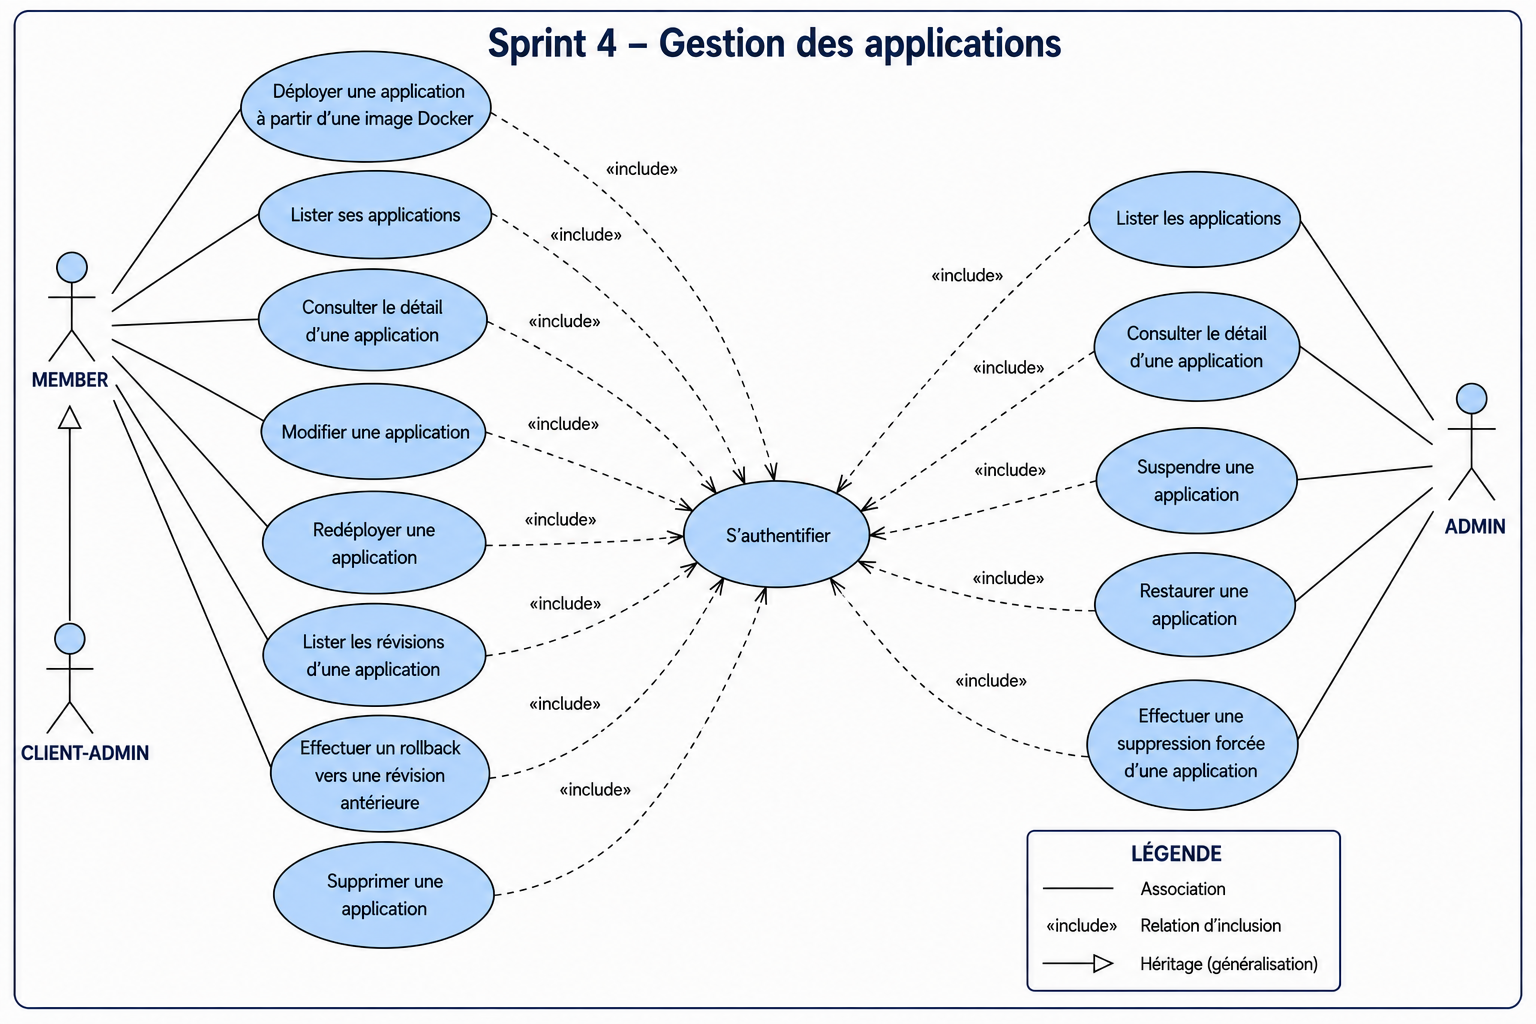
\includegraphics[width=0.95\textwidth]{image/uc-sprint4.png}
    \caption{Diagramme de cas d'utilisation du Sprint 4 — Gestion des applications}
    \label{fig:uc-sprint4}
\end{figure}

\subsection{Services Web}

\needspace{5cm}
\begin{longtable}{|p{6cm}|p{9.3cm}|}
\hline
Service Web & Description \\
\hline
\endfirsthead
\hline
Service Web & Description \\
\hline
\endhead
\hline
\endfoot
\endlastfoot
\texttt{POST /api/apps} & Déployer une application. \\ \hline
\texttt{GET /api/apps} & Lister ses applications. \\ \hline
\texttt{GET /api/apps/\{id\}} & Détail d'une application. \\ \hline
\texttt{POST /api/apps/\{id\}/deploy} & Redéployer une application existante. \\ \hline
\texttt{PUT /api/apps/\{id\}} & Modifier une application. \\ \hline
\texttt{DELETE /api/apps/\{id\}} & Supprimer une application. \\ \hline
\texttt{GET /api/apps/\{id\}/revisions} & Lister les révisions. \\ \hline
\texttt{POST /api/apps/\{id\}/rollback/\{revisionName\}} & Revenir à une révision antérieure. \\ \hline
\texttt{GET /api/admin/apps} & Lister toutes les applications, tous locataires confondus (ADMIN). \\ \hline
\texttt{DELETE /api/admin/apps/\{id\}} & Suppression forcée (ADMIN). \\ \hline
\texttt{POST /api/admin/apps/\{id\}/suspend} & Suspendre une application (ADMIN). \\ \hline
\texttt{POST /api/admin/apps/\{id\}/restore} & Restaurer une application suspendue (ADMIN). \\ \hline
\end{longtable}

\subsection{Conception}

Deux fonctionnalités sont détaillées : le déploiement, cœur fonctionnel du sprint et de la plateforme ; le retour à une révision antérieure, scénario opérationnel distinctif.

\subsubsection{Cas d'utilisation : « Déployer une application »}

\subsubsection*{Description textuelle}

\renewcommand{\arraystretch}{1.5}
\begin{longtable}{|p{4cm}|p{11cm}|}
\hline
Nom & Déployer une application \\
\hline
Acteur & CLIENT\_ADMIN, MEMBER (avec permission de déploiement) \\
\hline
Pré-condition & L'utilisateur est authentifié et dispose de la permission de déploiement \\
\hline
Scénario nominal & 1. L'utilisateur renseigne le formulaire de déploiement (nom, image, port, ressources, bornes de mise à l'échelle). 2. L'application est créée avec un statut de déploiement en cours. 3. Le backend répond immédiatement, puis déclenche de manière asynchrone la création de la ressource Knative correspondante. 4. Le statut de l'application est mis à jour en temps réel à mesure que Knative provisionne le service. \\
\hline
Post-condition & L'application est déployée et accessible, ou son statut reflète l'échec du déploiement. \\
\hline
\caption{Description textuelle du cas d'utilisation « Déployer une application »}
\label{tab:uc-deploy}
\end{longtable}

\subsubsection*{Diagramme de séquence}

\begin{figure}[H]
 \centering
    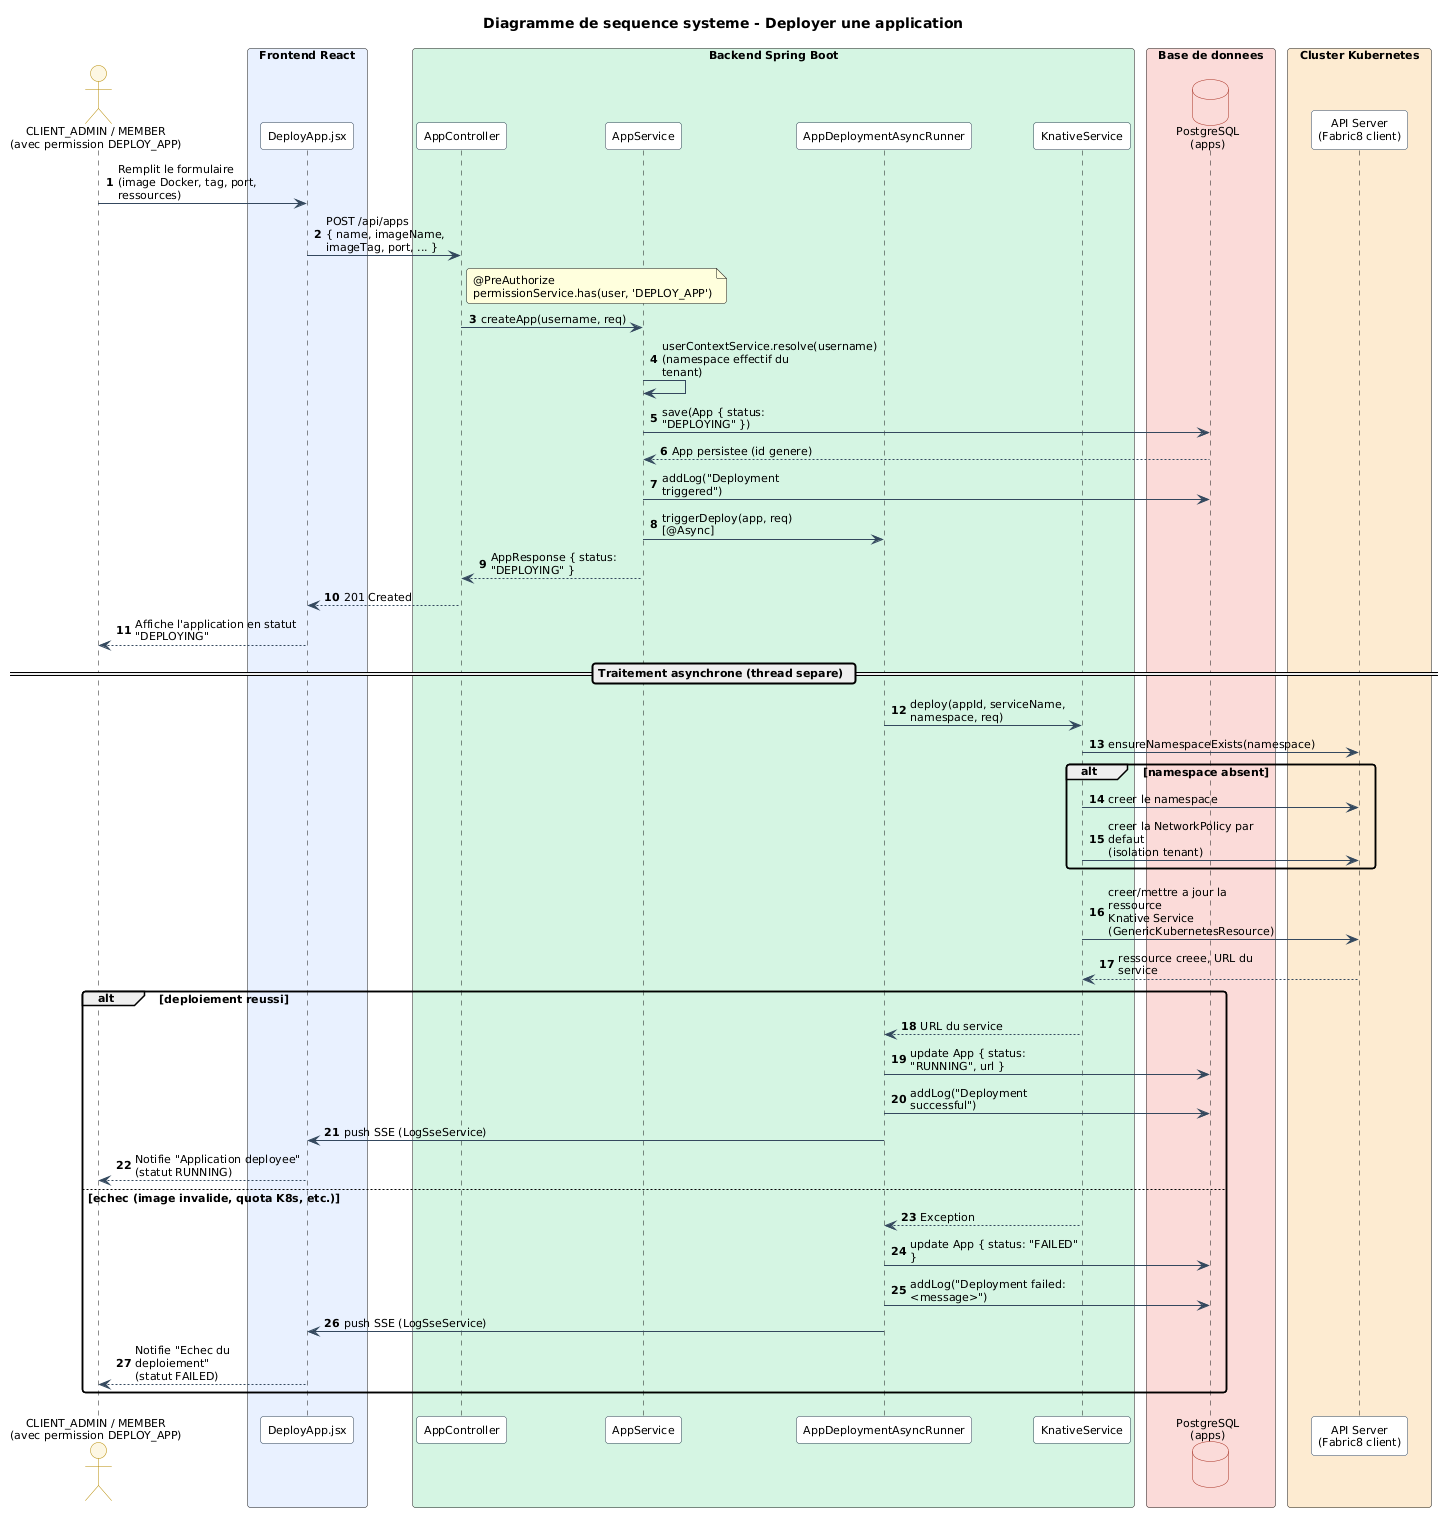
\includegraphics[width=\textwidth,height=0.85\textheight,keepaspectratio]{image/seq-deploy.png}
    \caption{Diagramme de séquence — Déployer une application}
    \label{fig:seq-deploy}
\end{figure}

\subsubsection{Cas d'utilisation : « Revenir à une révision antérieure »}

\subsubsection*{Description textuelle}

\renewcommand{\arraystretch}{1.5}
\begin{longtable}{|p{4cm}|p{11cm}|}
\hline
Nom & Revenir à une révision antérieure \\
\hline
Acteur & CLIENT\_ADMIN, MEMBER (avec permission de déploiement) \\
\hline
Pré-condition & L'application dispose d'au moins deux révisions \\
\hline
Scénario nominal & 1. L'utilisateur consulte l'historique des révisions de son application. 2. Il sélectionne une révision antérieure. 3. Le backend fait pointer le trafic Knative vers cette révision. \\
\hline
Post-condition & L'application sert à nouveau le comportement de la révision sélectionnée. \\
\hline
\caption{Description textuelle du cas d'utilisation « Revenir à une révision antérieure »}
\label{tab:uc-rollback}
\end{longtable}

\subsubsection*{Diagramme de séquence}

\begin{figure}[H]
 \centering
    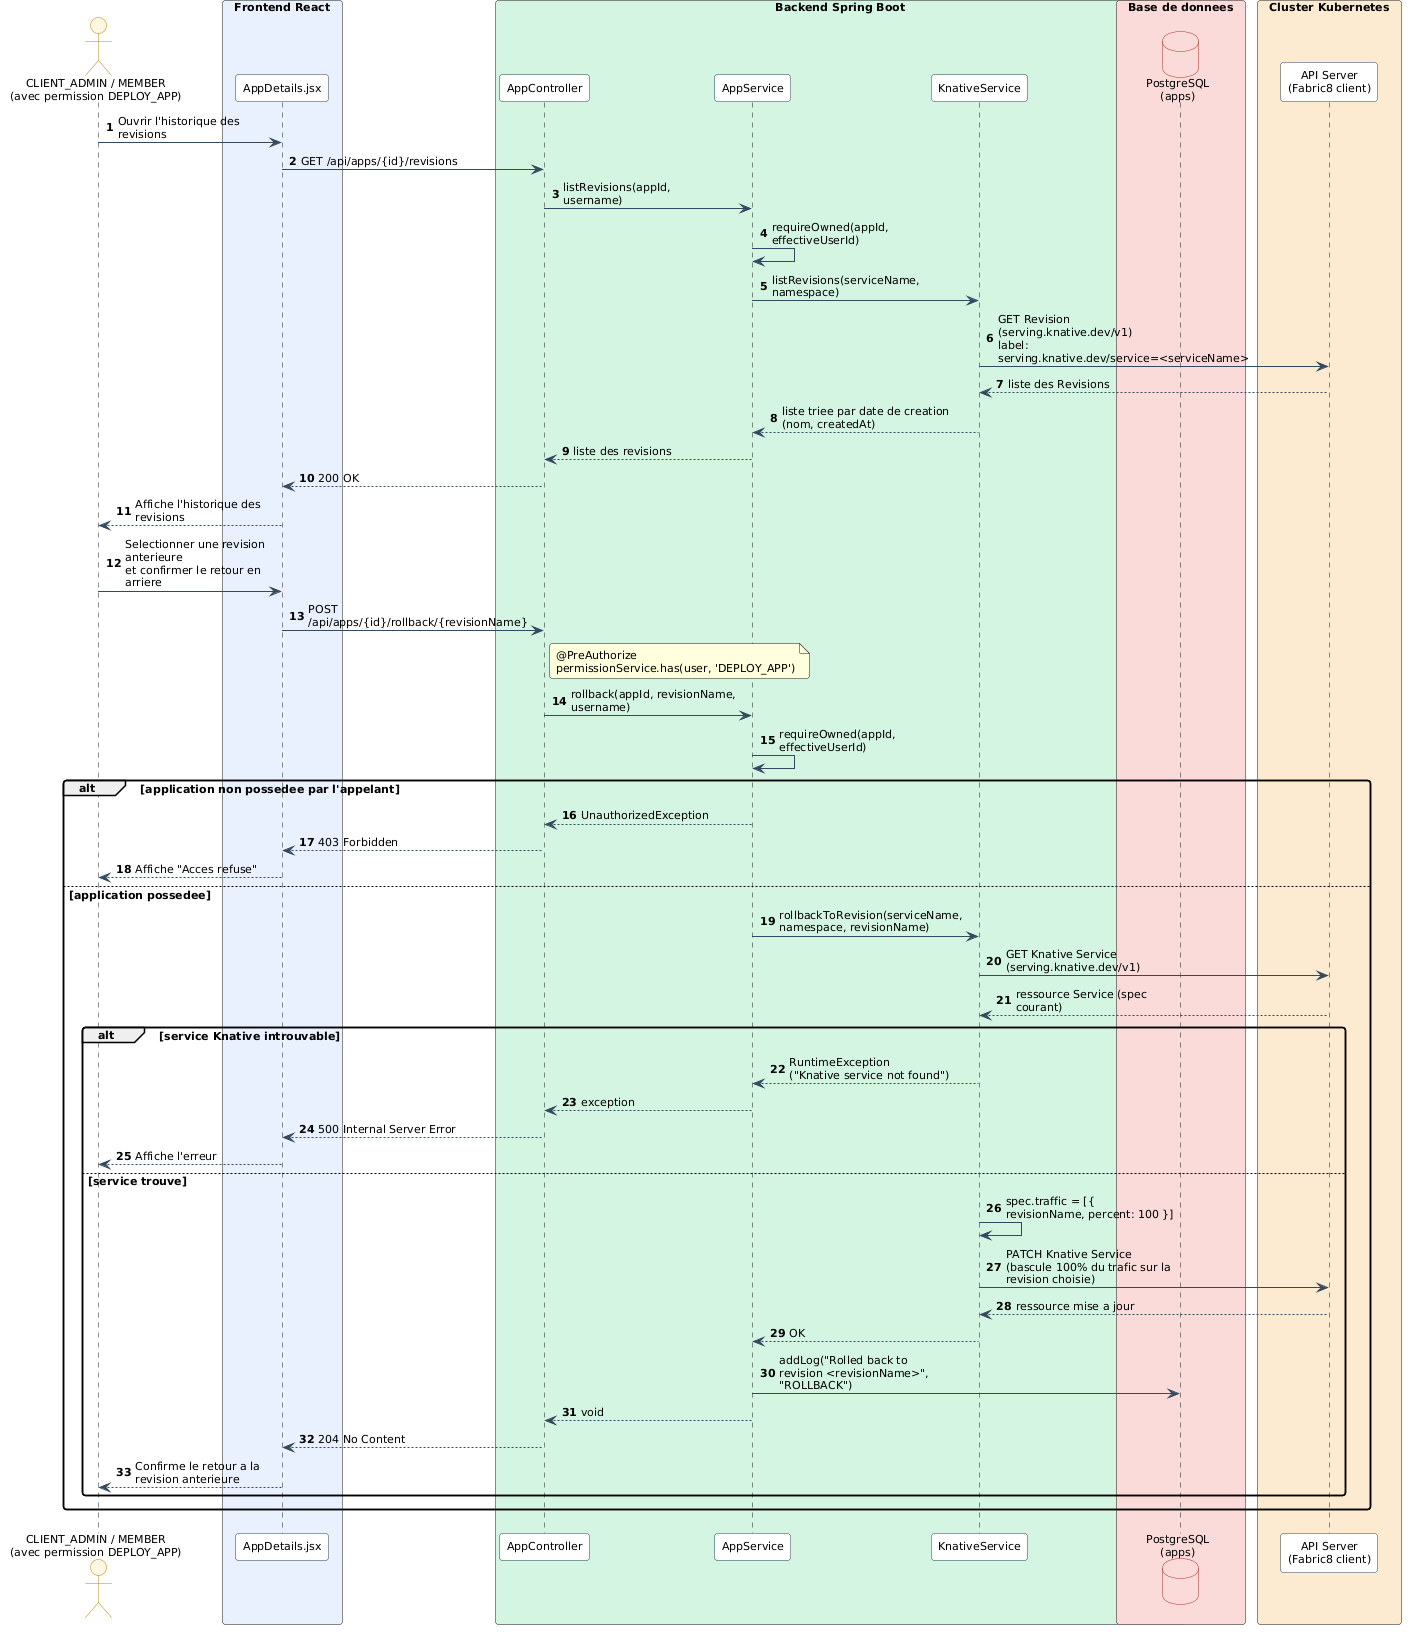
\includegraphics[width=\textwidth,height=0.85\textheight,keepaspectratio]{image/seq-rollback.png}
    \caption{Diagramme de séquence — Revenir à une révision antérieure}
    \label{fig:seq-rollback}
\end{figure}

\subsection{Réalisation du Sprint 4}

Fonctionnalité : Déployer une application. Le formulaire de déploiement du portail permet de créer une application à partir d'une image Docker.

\begin{figure}[H]
 \centering
    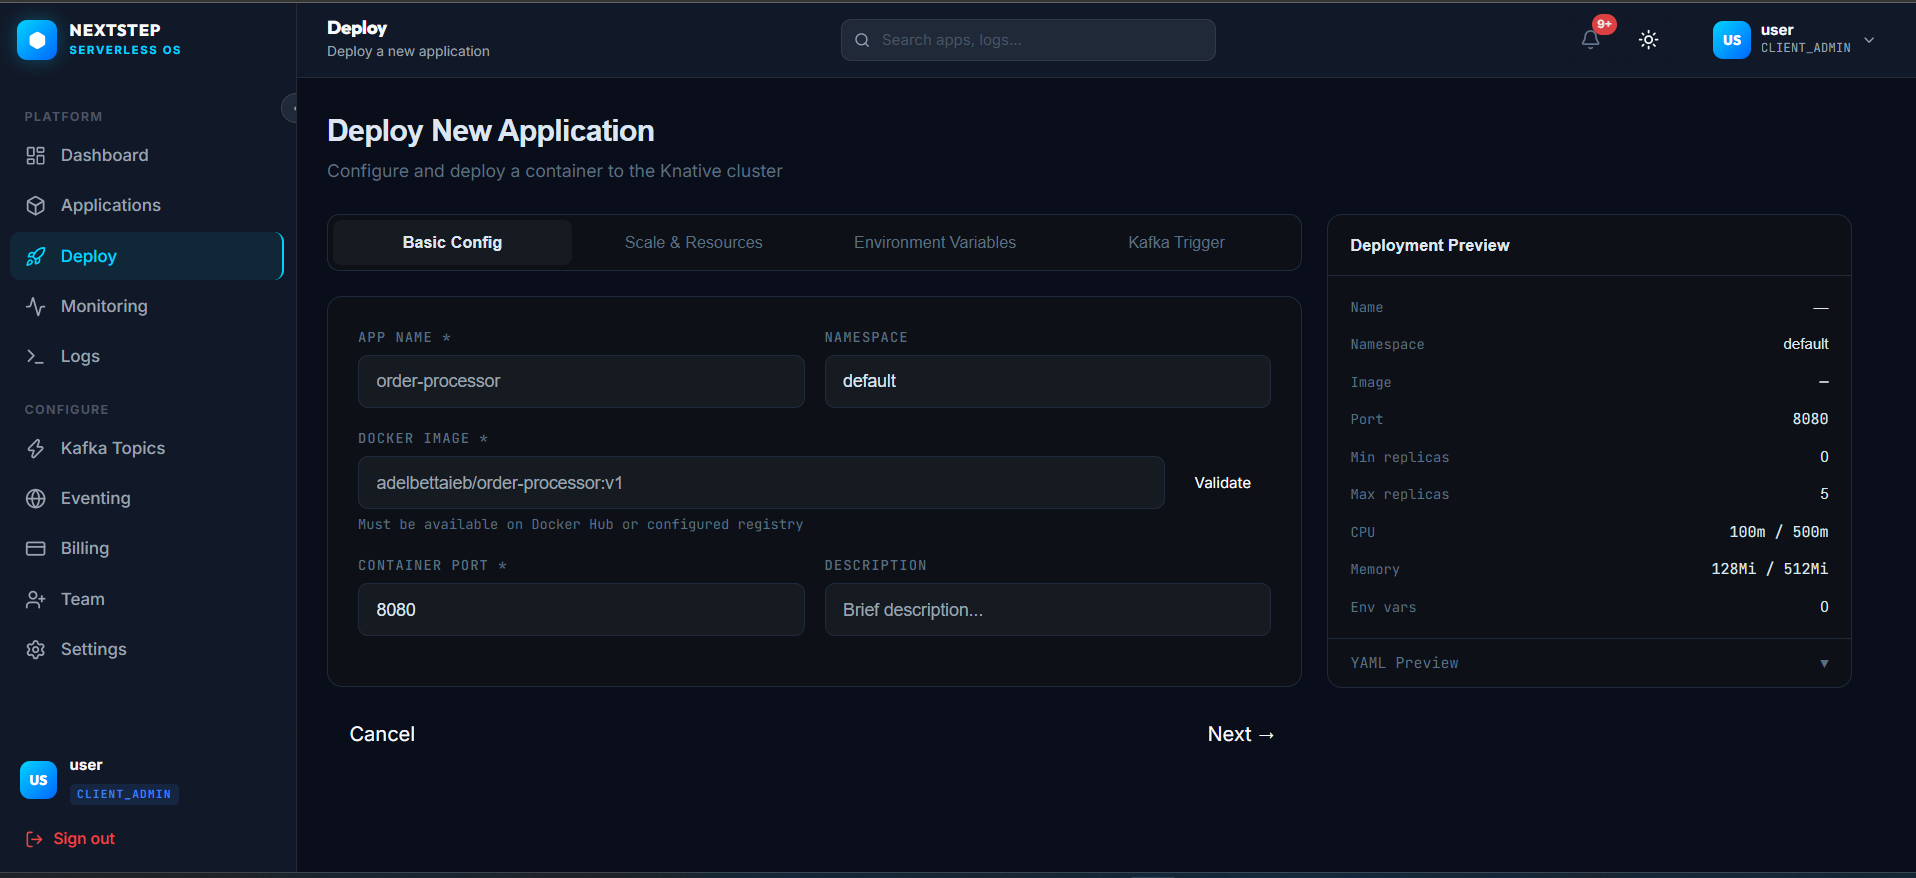
\includegraphics[width=\textwidth]{image/capture-deploy.png}
    \caption{Formulaire de déploiement d'une application}
    \label{fig:capture-deploy}
\end{figure}

Fonctionnalité : Consulter ses applications et leur statut. Le tableau de bord liste les applications du compte avec leur statut, synchronisé en temps réel depuis le cluster.

\begin{figure}[H]
 \centering
    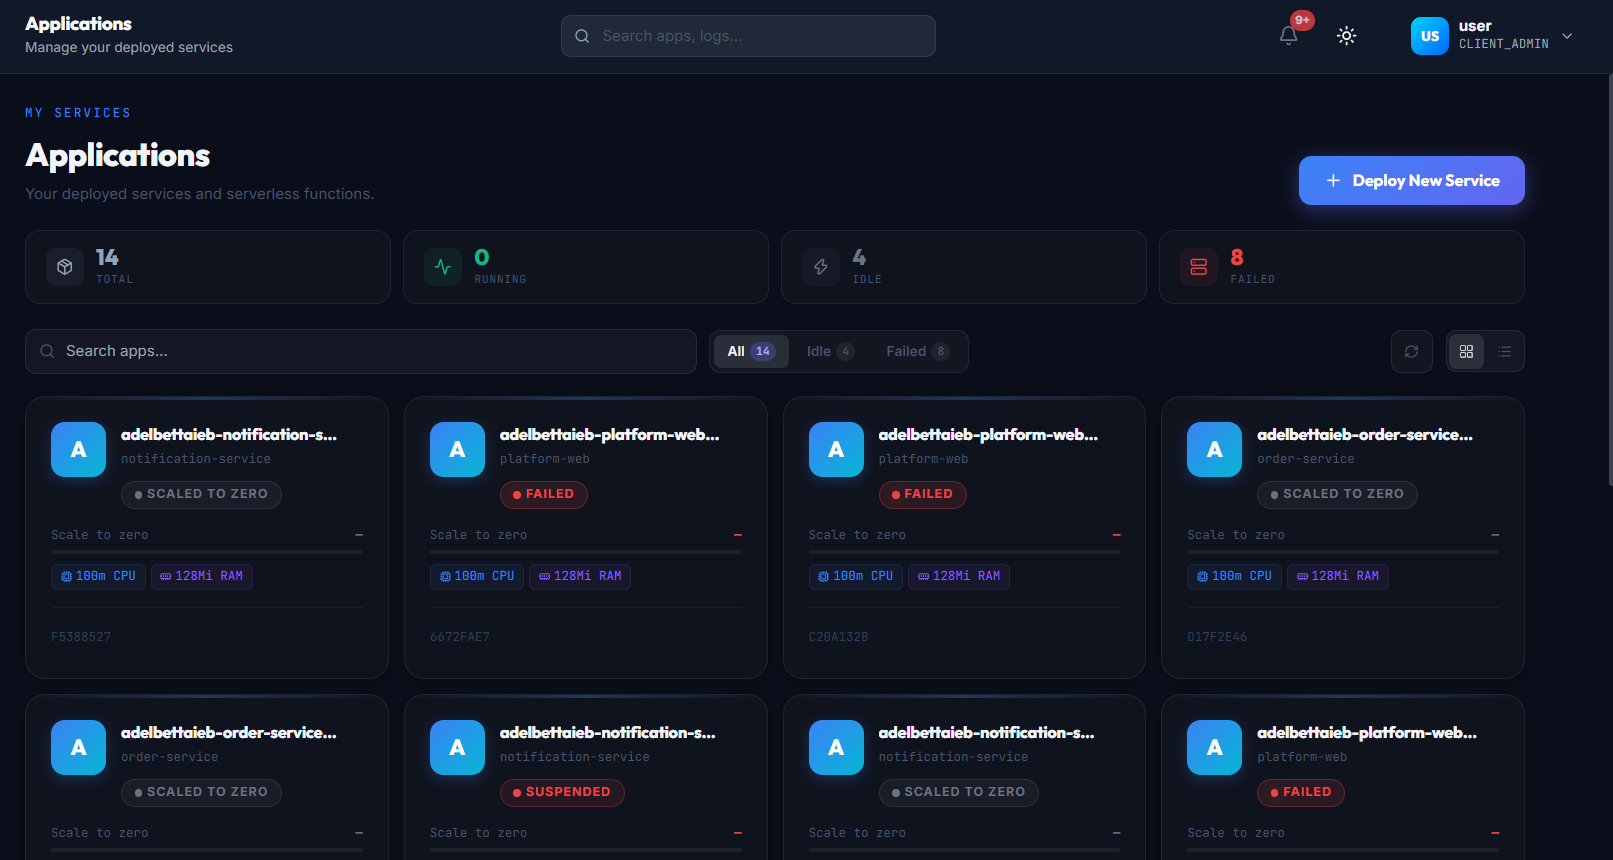
\includegraphics[width=\textwidth]{image/capture-appslist.png}
    \caption{Liste des applications et de leur statut}
    \label{fig:capture-appslist}
\end{figure}

Fonctionnalité : Modifier, redéployer ou supprimer une application. La page de détail d'une application permet de la modifier, de la redéployer ou de la supprimer.

Fonctionnalité : Consulter l'historique des révisions et revenir en arrière. L'historique des révisions et le retour à une version antérieure sont accessibles depuis la page de détail.

Fonctionnalité : Suspendre ou supprimer de force une application (ADMIN). L'ADMIN dispose, depuis la console d'administration, d'actions de suspension et de suppression forcée sur n'importe quelle application.

\EmplacementFigure{13cm}{8cm}{Actions administratives sur une application}{fig:capture-adminapps}

Au-delà du scénario nominal, le déploiement peut, si le formulaire renseigne un sujet Kafka, câbler automatiquement l'application créée à ce sujet, sans étape manuelle supplémentaire : ce chemin optionnel est décrit avec la gestion de la messagerie événementielle (Sprint 5), dont il anticipe la fonctionnalité de configuration d'un déclencheur.

\subsection{Conclusion}

Ce sprint livre le cycle de vie complet de gestion d'une application, accessible depuis le portail, avec un déploiement asynchrone et un suivi de statut en temps réel. La gestion des applications sert de socle à la messagerie événementielle et à l'observabilité applicative, objets des deux sprints suivants.

\clearpage
\section{Sprint 5 : Gestion de la messagerie événementielle}

\subsection{Introduction}

Ce sprint livre, comme un seul domaine fonctionnel, la gestion des sujets Kafka et la configuration des déclencheurs qui relient un sujet à une application : la publication d'un message sur un sujet réveille alors automatiquement l'application concernée. Ces deux briques, Kafka (Strimzi) et Knative Eventing, ne prennent leur sens qu'ensemble ; les traiter comme un seul sprint évite de les documenter à deux endroits distincts.

\subsection{Sprint Backlog}

Le tableau~\ref{tab:sb-sprint5} présente le backlog détaillé du Sprint 5, obtenu en décomposant chaque User Story retenue en tâches techniques.

\needspace{0.9\textheight}
{
\setlength{\LTleft}{-1.5cm}
\setlength{\LTright}{-1.5cm}
\setlength{\tabcolsep}{8pt}
\renewcommand{\arraystretch}{1.9}
\begin{longtable}{|p{6.6cm}|>{\raggedright\arraybackslash}p{8.1cm}|>{\centering\arraybackslash}p{2.3cm}|}
\hline
User Story & Tâches & Estimation \\
\hline
\endfirsthead
\hline
User Story & Tâches & Estimation \\
\hline
\endhead
\hline
\endfoot

\caption{Backlog du Sprint 5}
\label{tab:sb-sprint5}
\endlastfoot

\multirow{4}{6.6cm}{\centering En tant que CLIENT\_ADMIN ou MEMBER (avec permission MANAGE\_KAFKA), je veux créer et gérer des sujets Kafka afin d'y publier des événements.}
& Développer la création d'un sujet Kafka. & 1 \\* \cline{2-3}
& Développer la liste et le détail d'un sujet. & 1 \\* \cline{2-3}
& Développer la suppression d'un sujet. & 1 \\* \cline{2-3}
& Développer la page de gestion des sujets Kafka. & 1 \\ \hline

\multirow{5}{6.6cm}{\centering En tant que CLIENT\_ADMIN ou MEMBER (avec permission MANAGE\_EVENTING), je veux relier un sujet Kafka à une application afin qu'elle soit réveillée automatiquement à la réception d'un message.}
& Développer la création d'une KafkaSource. & 1 \\* \cline{2-3}
& Développer la création d'un Trigger. & 1 \\* \cline{2-3}
& Développer la suppression d'un Trigger. & 1 \\* \cline{2-3}
& Développer la page de configuration des déclencheurs. & 1 \\* \cline{2-3}
& Tester le déclenchement d'une application. & 1 \\ \hline

\multirow{2}{6.6cm}{\centering En tant que CLIENT\_ADMIN ou MEMBER, je veux publier un événement sur un sujet afin de déclencher un traitement.}
& Développer l'API de publication d'un événement. & 1 \\* \cline{2-3}
& Tester la publication d'un événement. & 1 \\ \hline

\multirow{3}{6.6cm}{\centering En tant qu'ADMIN, je veux consulter l'ensemble des sujets, sources et déclencheurs de tous les clients, et supprimer un sujet de force, afin de gérer les abus.}
& Développer la vue globale des sujets, sources et déclencheurs. & 1 \\* \cline{2-3}
& Développer la suppression forcée d'un sujet. & 1 \\* \cline{2-3}
& Tester ces actions. & 1 \\ \hline

\end{longtable}
}

\subsection{Diagramme de cas d'utilisation du Sprint 5}

Le diagramme réunit CLIENT\_ADMIN et MEMBER (sous permission \texttt{MANAGE\_KAFKA}/\texttt{MANAGE\_EVENTING}), ainsi qu'ADMIN, avec l'ensemble des fonctionnalités du sprint.

\begin{figure}[H]
 \centering
    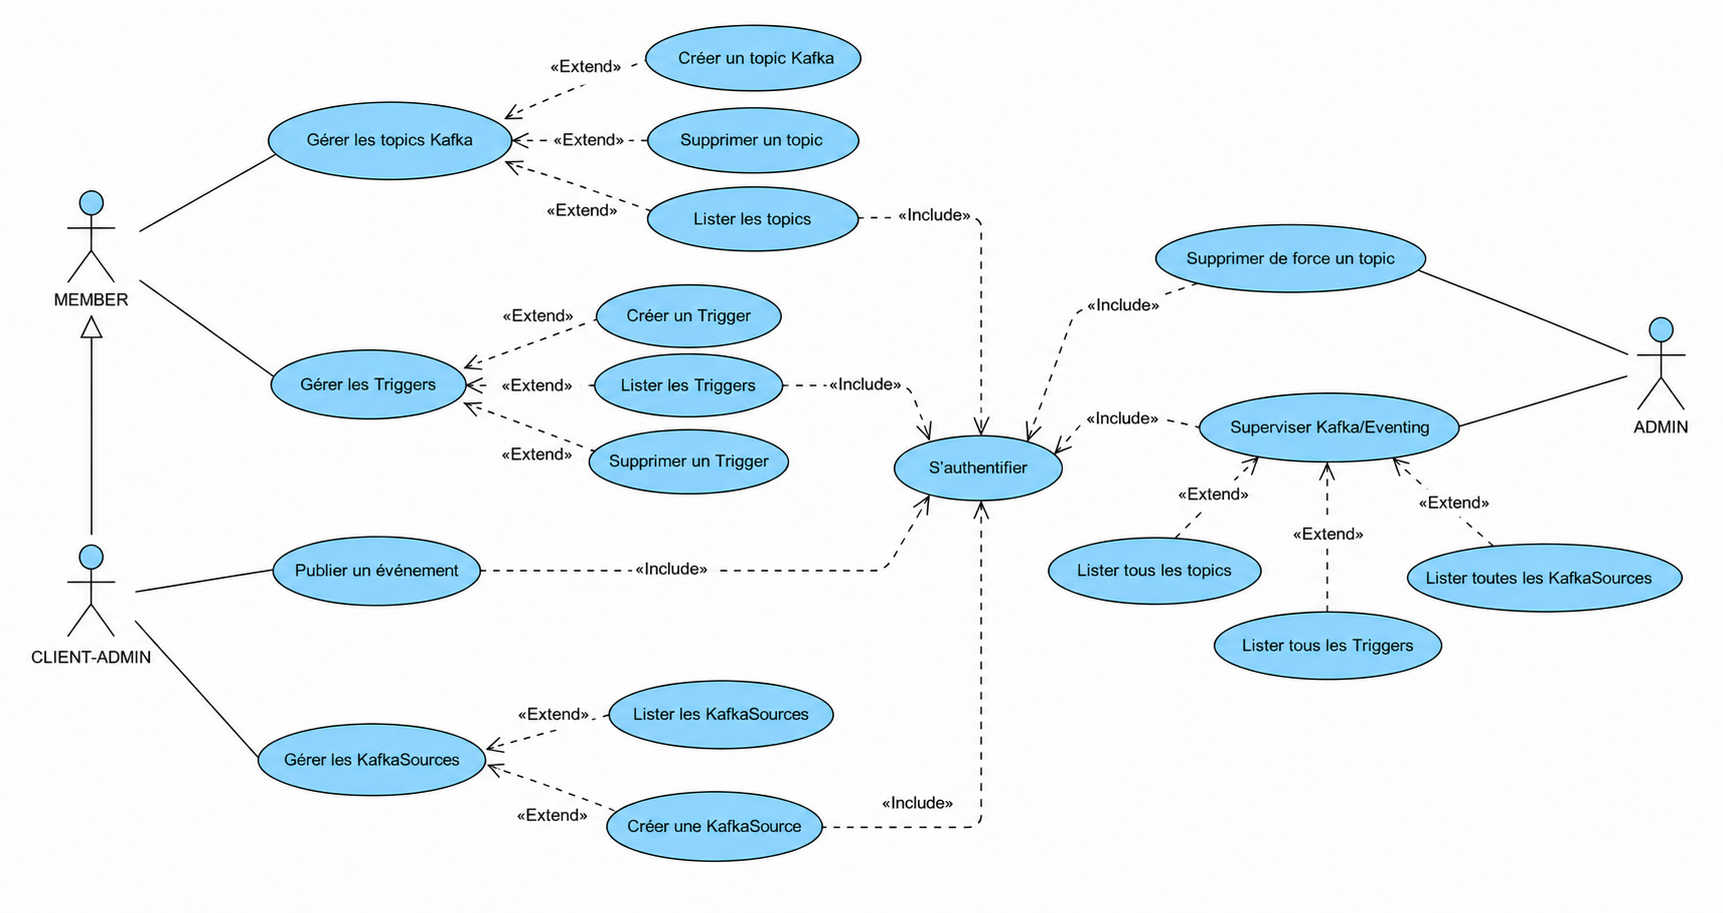
\includegraphics[width=\textwidth]{image/Sprint5usescase.png}
    \caption{Diagramme de cas d'utilisation du Sprint 5 — Gestion de la messagerie événementielle}
    \label{fig:uc-sprint5}
\end{figure}


\subsection{Services Web}

\needspace{5cm}
\begin{longtable}{|p{6cm}|p{9.3cm}|}
\hline
Service Web & Description \\
\hline
\endfirsthead
\hline
Service Web & Description \\
\hline
\endhead
\hline
\endfoot
\endlastfoot
\texttt{POST /api/kafka/topics} & Créer un sujet Kafka. \\ \hline
\texttt{GET /api/kafka/topics} & Lister ses sujets. \\ \hline
\texttt{GET /api/kafka/topics/\{id\}} & Détail d'un sujet. \\ \hline
\texttt{DELETE /api/kafka/topics/\{id\}} & Supprimer un sujet. \\ \hline
\texttt{POST /api/eventing/sources} & Créer une KafkaSource. \\ \hline
\texttt{GET /api/eventing/sources} & Lister ses KafkaSource. \\ \hline
\texttt{POST /api/eventing/triggers} & Créer un déclencheur (Trigger). \\ \hline
\texttt{GET /api/eventing/triggers} & Lister ses déclencheurs. \\ \hline
\texttt{DELETE /api/eventing/triggers/\{id\}} & Supprimer un déclencheur. \\ \hline
\texttt{POST /api/events} & Publier un événement (CloudEvent). \\ \hline
\texttt{GET /api/admin/kafka/topics} & Lister tous les sujets, tous locataires confondus (ADMIN). \\ \hline
\texttt{DELETE /api/admin/kafka/topics/\{id\}} & Suppression forcée d'un sujet (ADMIN). \\ \hline
\texttt{GET /api/admin/eventing/sources}, \texttt{/triggers} & Vue globale des sources et déclencheurs (ADMIN). \\ \hline
\end{longtable}

\subsection{Conception}

Une fonctionnalité est détaillée : la configuration d'un déclencheur, la plus riche techniquement puisqu'elle relie deux briques indépendantes du socle (Kafka et Knative).

\subsubsection{Cas d'utilisation : « Configurer un déclencheur d'événement »}

\subsubsection*{Description textuelle}

\renewcommand{\arraystretch}{1.5}
\begin{longtable}{|p{4cm}|p{11cm}|}
\hline
Nom & Configurer un déclencheur d'événement \\
\hline
Acteur & CLIENT\_ADMIN, MEMBER (avec permission de gestion de l'Eventing) \\
\hline
Pré-condition & L'application cible est déployée ; le sujet Kafka source existe \\
\hline
Scénario nominal & 1. L'utilisateur sélectionne un sujet Kafka et une application cible. 2. Le backend crée la ressource KafkaSource rattachée au sujet. 3. Le backend crée la ressource Trigger associée, filtrant sur le type d'événement et pointant vers l'URL du service Knative de l'application. 4. La configuration est persistée et son état est renvoyé à l'utilisateur. \\
\hline
Post-condition & Toute publication ultérieure sur le sujet Kafka déclenche, le cas échéant, le réveil et l'invocation de l'application. \\
\hline
\caption{Description textuelle du cas d'utilisation « Configurer un déclencheur d'événement »}
\label{tab:uc-eventing}
\end{longtable}

Ce processus, du message Kafka au réveil et au traitement par l'application, est illustré à la figure~\ref{fig:seq-eventing}.

\begin{figure}[H]
\begin{adjustwidth}{-1.3cm}{-1.3cm}
\centering
\begin{tikzpicture}[
  x=1cm, y=1cm,
  every node/.style={font=\normalsize},
  act/.style={draw=black!60, line width=1pt, rounded corners, minimum width=5.4cm,
              minimum height=1.3cm, align=center, fill=black!5},
  don/.style={draw=figBleu, line width=1pt, rounded corners, minimum width=5.4cm,
              minimum height=1.3cm, align=center, fill=figBleuFond},
  eta/.style={draw=figVert, line width=1pt, rounded corners, minimum width=5.4cm,
              minimum height=1.3cm, align=center, fill=figVertFond},
  ctl/.style={draw=figOrange, line width=1pt, dashed, rounded corners, minimum width=5.0cm,
              minimum height=1.3cm, align=center, fill=figOrangeFond},
  num/.style={circle, draw, line width=0.8pt, fill=white, inner sep=1.5pt, font=\small\bfseries},
  lbl/.style={font=\footnotesize},
  fl/.style={->, line width=1pt, figBleu},
  fv/.style={->, line width=1pt, figVert},
  fc/.style={->, line width=1pt, dashed, figOrange}
]

\node[act] (prod) at (0,0)     {Producteur\\[1pt]\small publie un message};
\node[don] (topic) at (0,-2.3)  {Sujet Kafka (cluster Strimzi)};
\node[don] (src)  at (0,-4.6)  {KafkaSource\\[1pt]\small consomme et encapsule en CloudEvent};
\node[don] (brk)  at (0,-6.9)  {Broker Knative Eventing};
\node[don] (trg)  at (0,-9.2)  {Trigger\\[1pt]\small filtre et route l'événement};
\node[eta] (pod)  at (0,-13.4) {Pod applicatif\\[1pt]\small traite l'événement, répond HTTP 200};
\node[eta] (fin)  at (0,-16.1) {Retour au repos\\[1pt]\small 0 instance après inactivité};

\node[ctl] (act)  at (9.4,-9.2)  {Activator\\[1pt]\small intercepte si 0 instance};
\node[ctl] (kpa)  at (9.4,-11.3) {Autoscaler (KPA)};
\node[ctl] (rev)  at (9.4,-13.4) {Revision $\rightarrow$ Deployment\\[1pt]\small réplicas 0 $\rightarrow$ 1};
\node[ctl] (down) at (9.4,-16.1) {Autoscaler\\[1pt]\small réplicas 1 $\rightarrow$ 0};

\draw[fl] (prod) -- (topic);
\draw[fl] (topic) -- (src);
\draw[fl] (src) -- (brk);
\draw[fl] (brk) -- (trg);
\draw[fl] (trg) -- (pod);
\draw[fc] (trg.east) -- (act.west);
\draw[fc] (act) -- (kpa);
\draw[fc] (kpa) -- (rev);
\draw[fl] (rev.west) -- (pod.east);
\draw[fv] (pod) -- (fin);
\draw[fc] (fin.east) -- (down.west);
\draw[fv] (down.east) -- (12.6,-16.1) |- (prod.east);

\node[num] at (0,-1.15) {1};
\node[num] at (0,-3.45) {2};
\node[num] at (0,-5.75) {3};
\node[num] at (0,-8.05) {4};
\node[num] at (4.7,-9.2)  {5};
\node[num] at (9.4,-10.25) {6};
\node[num] at (9.4,-12.35) {7};
\node[num] at (4.7,-13.05)  {8};
\node[num] at (0,-14.35)    {9};
\node[num] at (9.4,-14.75) {10};
\node[num] at (12.6,-4.6) {11};

\node[lbl, anchor=south] at (4.7,-9.0)  {si 0 instance};
\node[lbl, anchor=west] at (0.3,-5.75) {via HTTP};
\node[lbl, anchor=south] at (4.7,-12.85) {le Pod démarre};
\node[lbl] at (0,-15.15) {réponse HTTP 200};
\node[lbl, anchor=east]  at (9.1,-14.75) {inactivité prolongée};
\node[lbl, anchor=south, align=center] at (7.6,0.1) {nouveau message Kafka};

\end{tikzpicture}
\caption{Processus événementiel : d'un message Kafka au réveil et au traitement par l'application Knative}
\label{fig:seq-eventing}
\end{adjustwidth}
\end{figure}

\subsubsection*{Diagramme de séquence}

\begin{figure}[H]
 \centering
    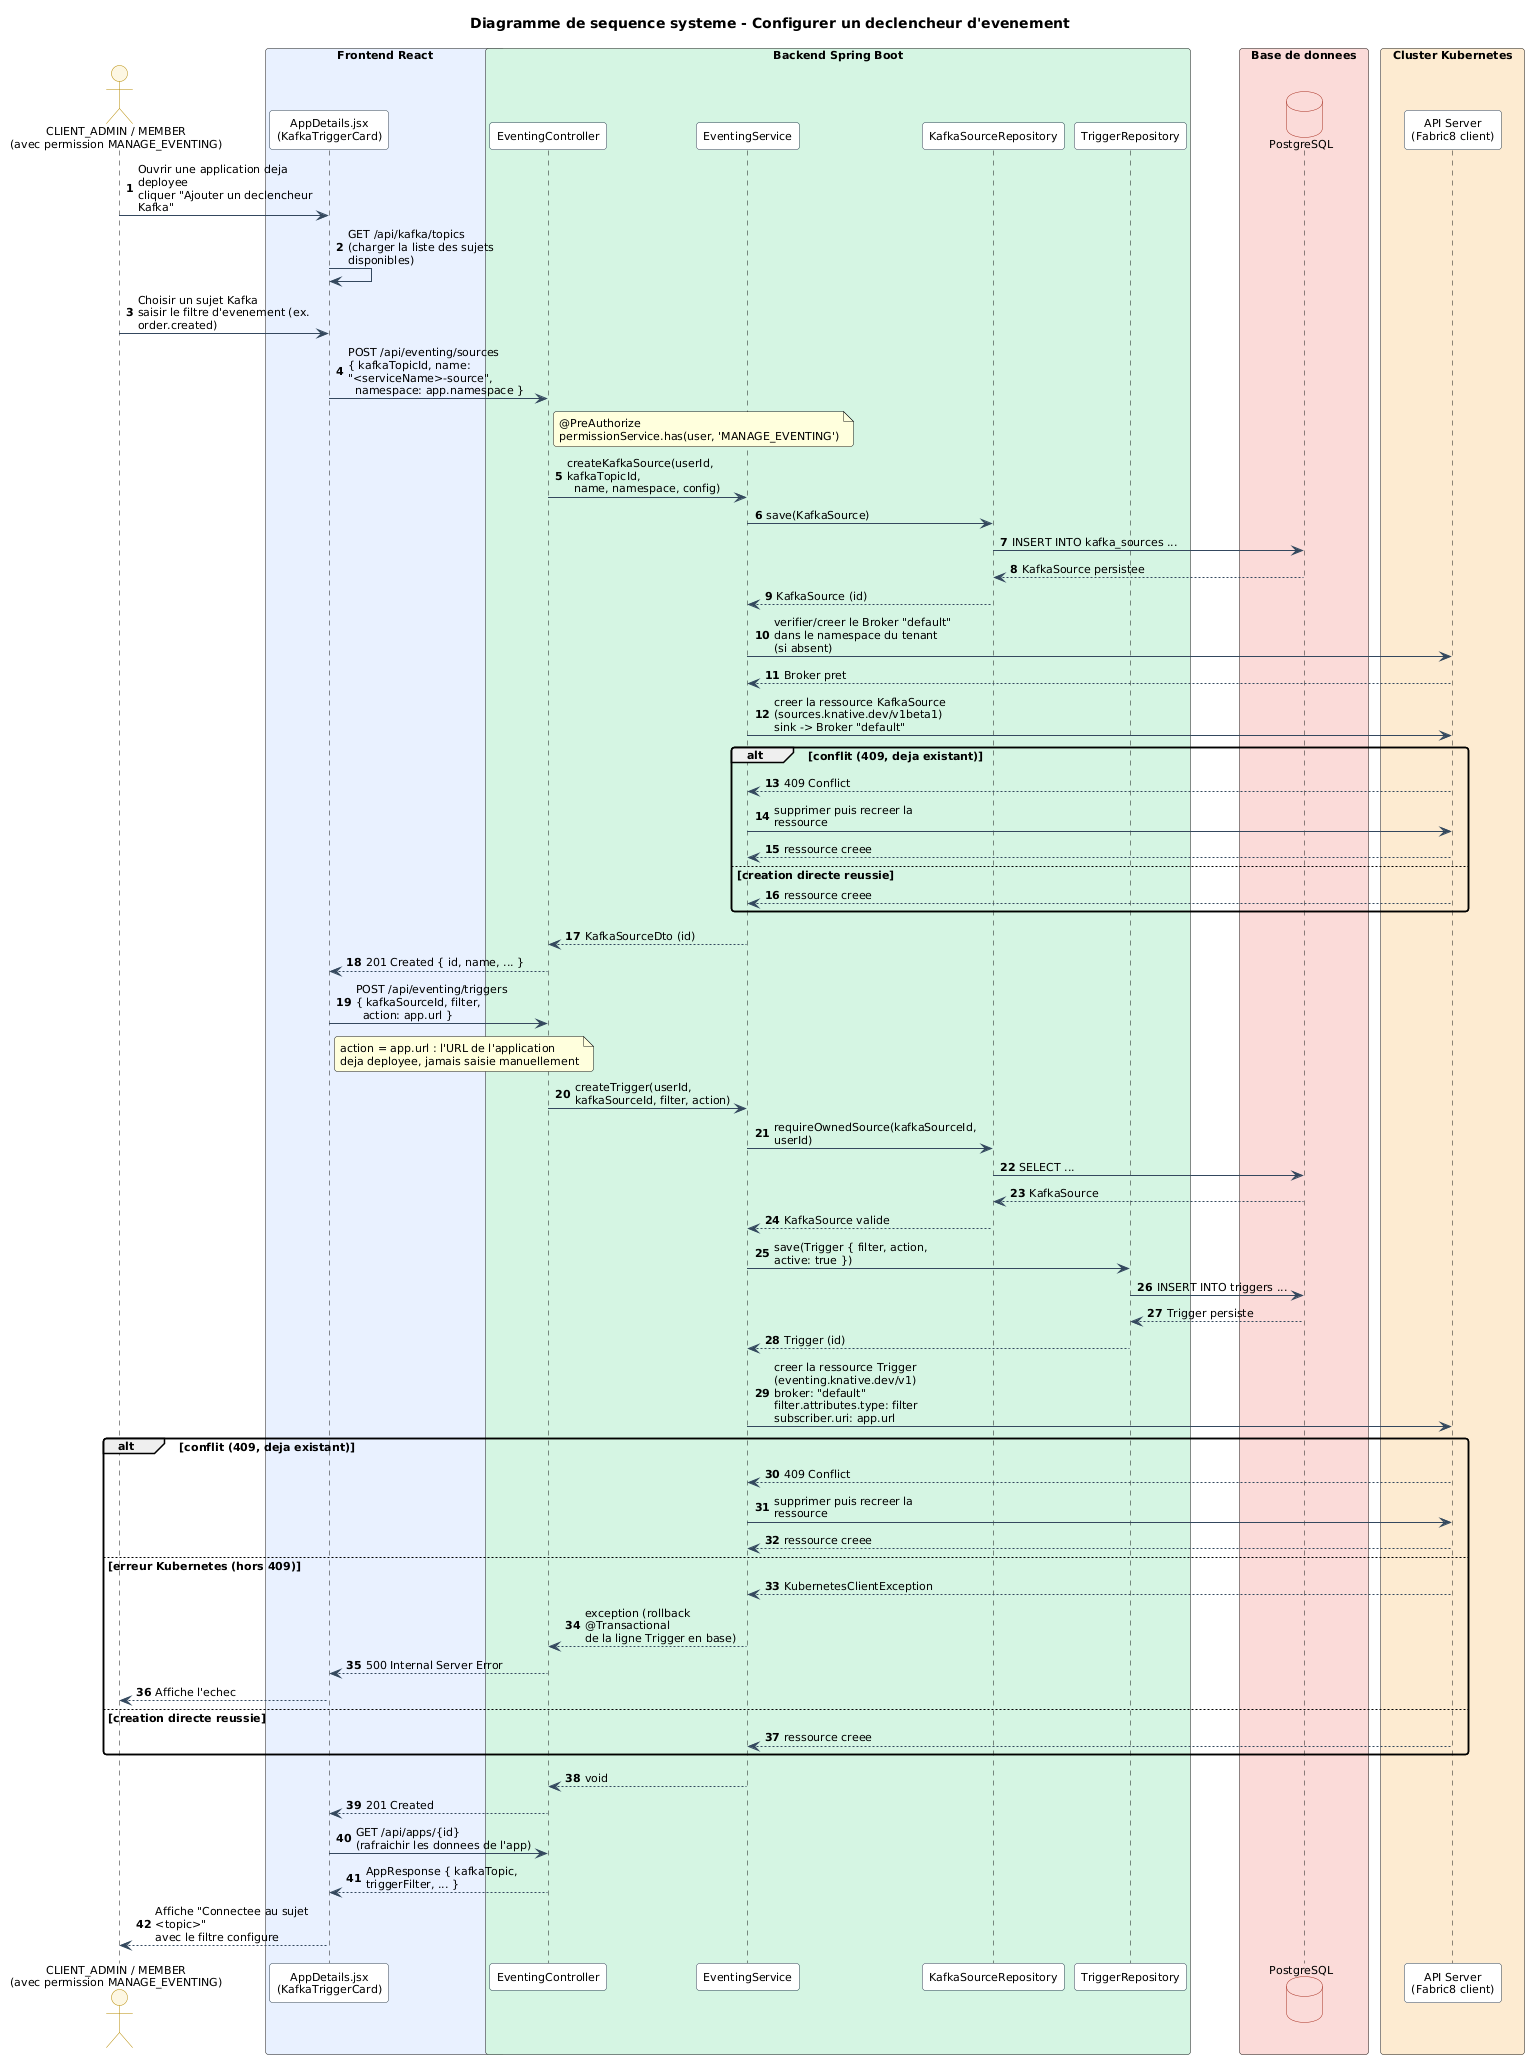
\includegraphics[width=\textwidth,height=0.85\textheight,keepaspectratio]{image/seq-eventing-trigger.png}
    \caption{Diagramme de séquence — Configurer un déclencheur d'événement}
    \label{fig:seq-eventing-trigger}
\end{figure}

\subsection{Réalisation du Sprint 5}

Fonctionnalité : Créer et gérer des sujets Kafka. La page de gestion Kafka du portail permet de créer, lister et supprimer les sujets du compte.

\begin{figure}[H]
 \centering
    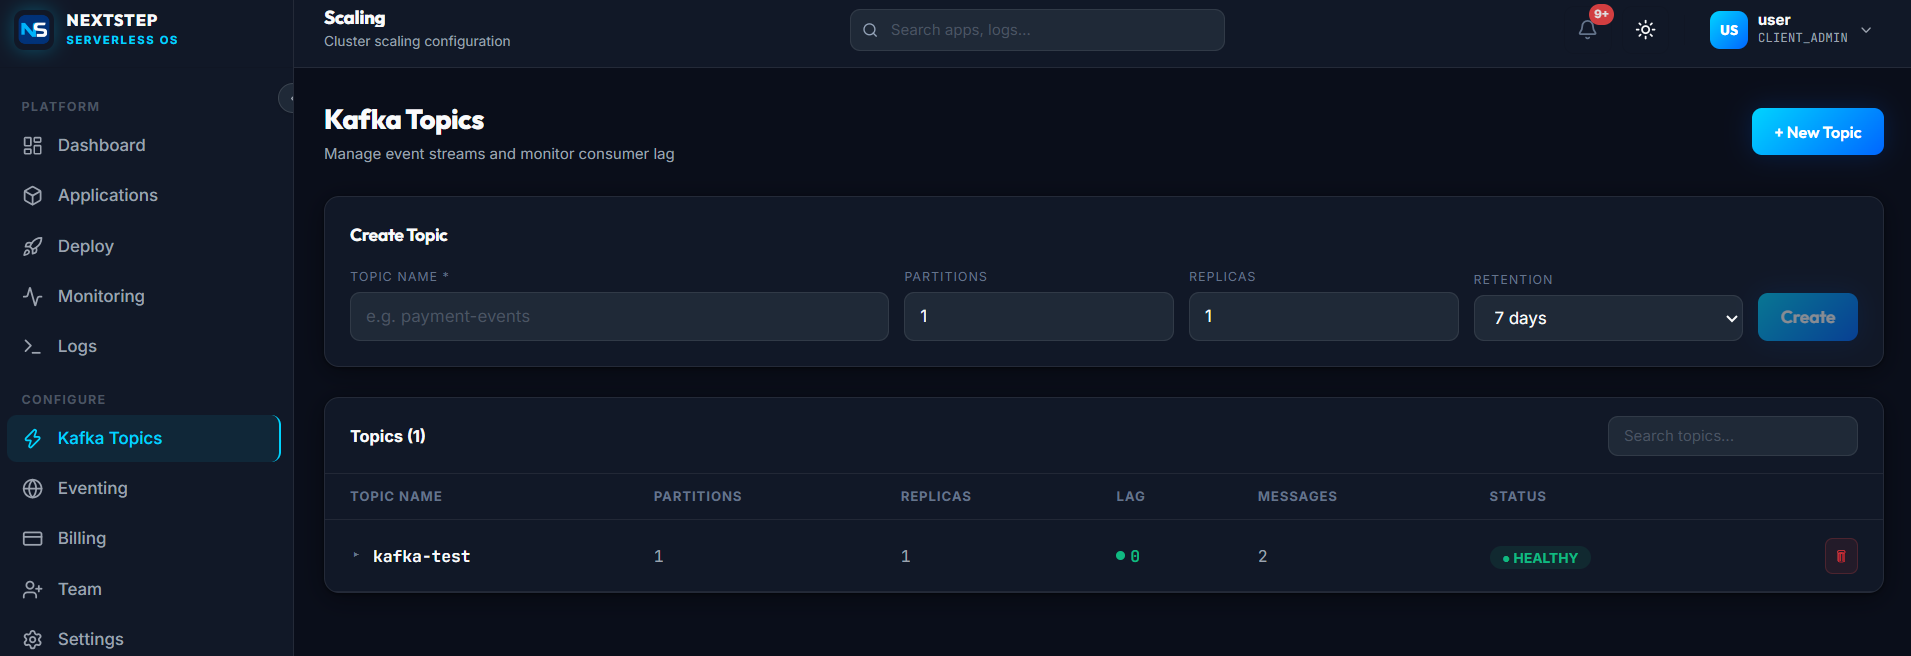
\includegraphics[width=0.9\textwidth]{image/Interface de gestion des sujets Kafka.png}
    \caption{Interface de gestion des sujets Kafka}
    \label{fig:capture-kafkatopics}
\end{figure}



Les trois ressources techniques que ce déclencheur assemble (Broker, KafkaSource, Trigger) sont visibles directement sur le cluster. La figure~\ref{fig:capture-eventing-broker} montre le Broker du tenant, à l'état prêt.

\begin{figure}[H]
 \centering
    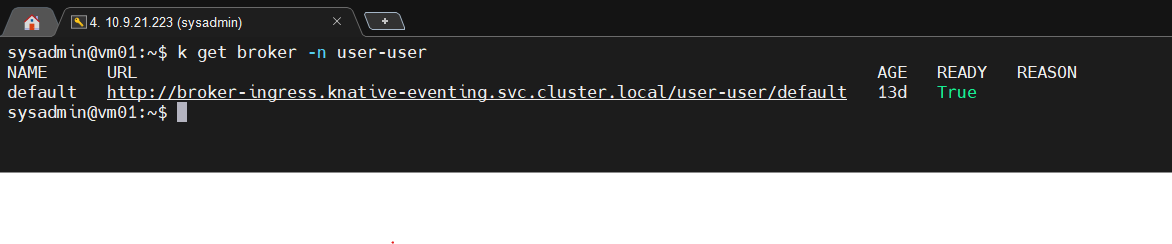
\includegraphics[width=0.92\textwidth]{image/capture_eventing_broker.png}
    \caption{Broker Knative Eventing du tenant}
    \label{fig:capture-eventing-broker}
\end{figure}

La figure~\ref{fig:capture-eventing-trigger} liste le Trigger créé pour une application : il référence le Broker et pointe vers l'URL du service cible.

\begin{figure}[H]
 \centering
    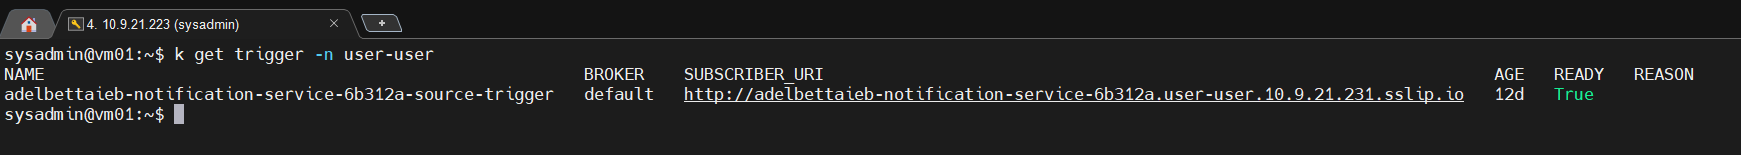
\includegraphics[width=0.92\textwidth]{image/capture_eventing_trigger.png}
    \caption{Trigger Knative Eventing associé à une application}
    \label{fig:capture-eventing-trigger}
\end{figure}

La figure~\ref{fig:capture-eventing-kafkasource} affiche la KafkaSource correspondante, qui consomme le sujet via le service de bootstrap du cluster Kafka.

\begin{figure}[H]
 \centering
    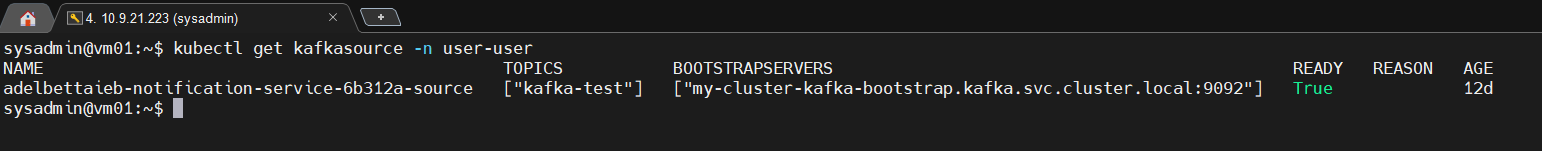
\includegraphics[width=0.92\textwidth]{image/capture_eventing_kafkasource.png}
    \caption{KafkaSource Knative Eventing associée au sujet Kafka}
    \label{fig:capture-eventing-kafkasource}
\end{figure}

Fonctionnalité : Publier un événement. Un CLIENT\_ADMIN ou un MEMBER publie un événement directement sur un sujet.

\begin{figure}[H]
 \centering
    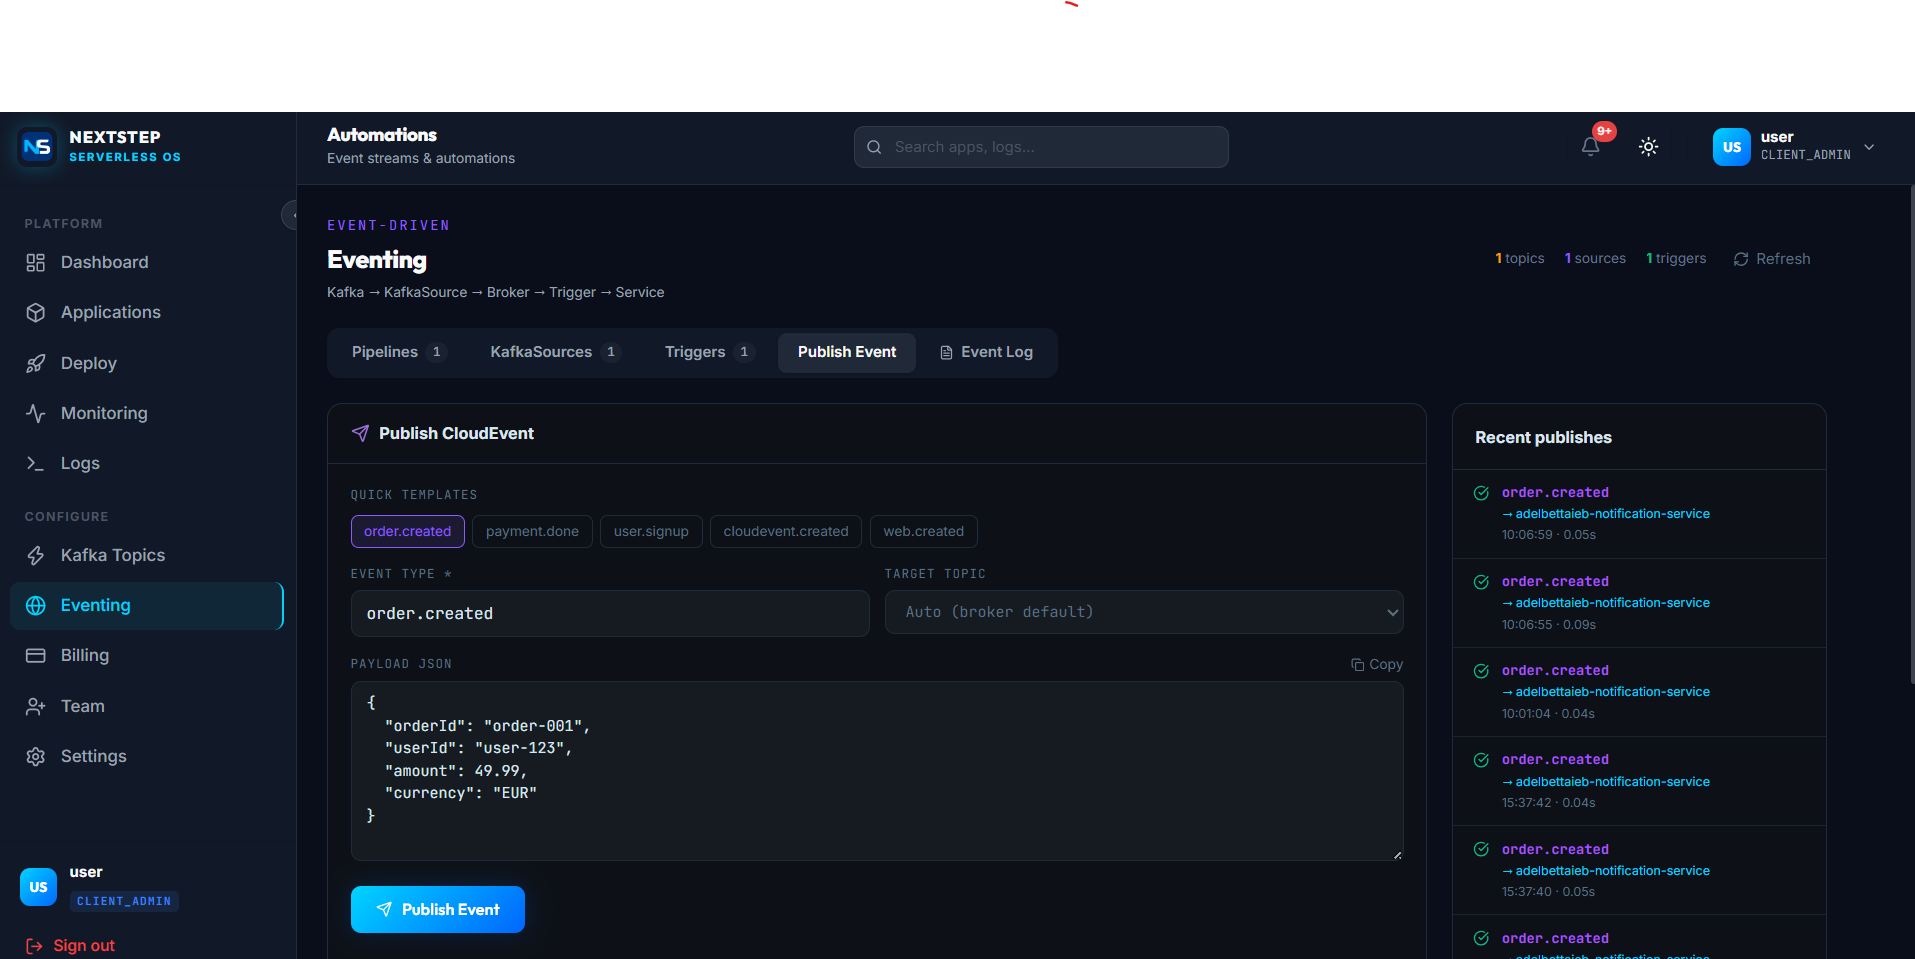
\includegraphics[width=0.9\textwidth]{image/Publication d’un événement.png}
    \caption{Publication d'un événement}
    \label{fig:capture-publish}
\end{figure}

Fonctionnalité : Vue globale et suppression forcée (ADMIN). L'ADMIN consulte, depuis la console d'administration, l'ensemble des sujets, sources et déclencheurs de tous les clients, et peut supprimer un sujet de force.

\begin{figure}[H]
 \centering
    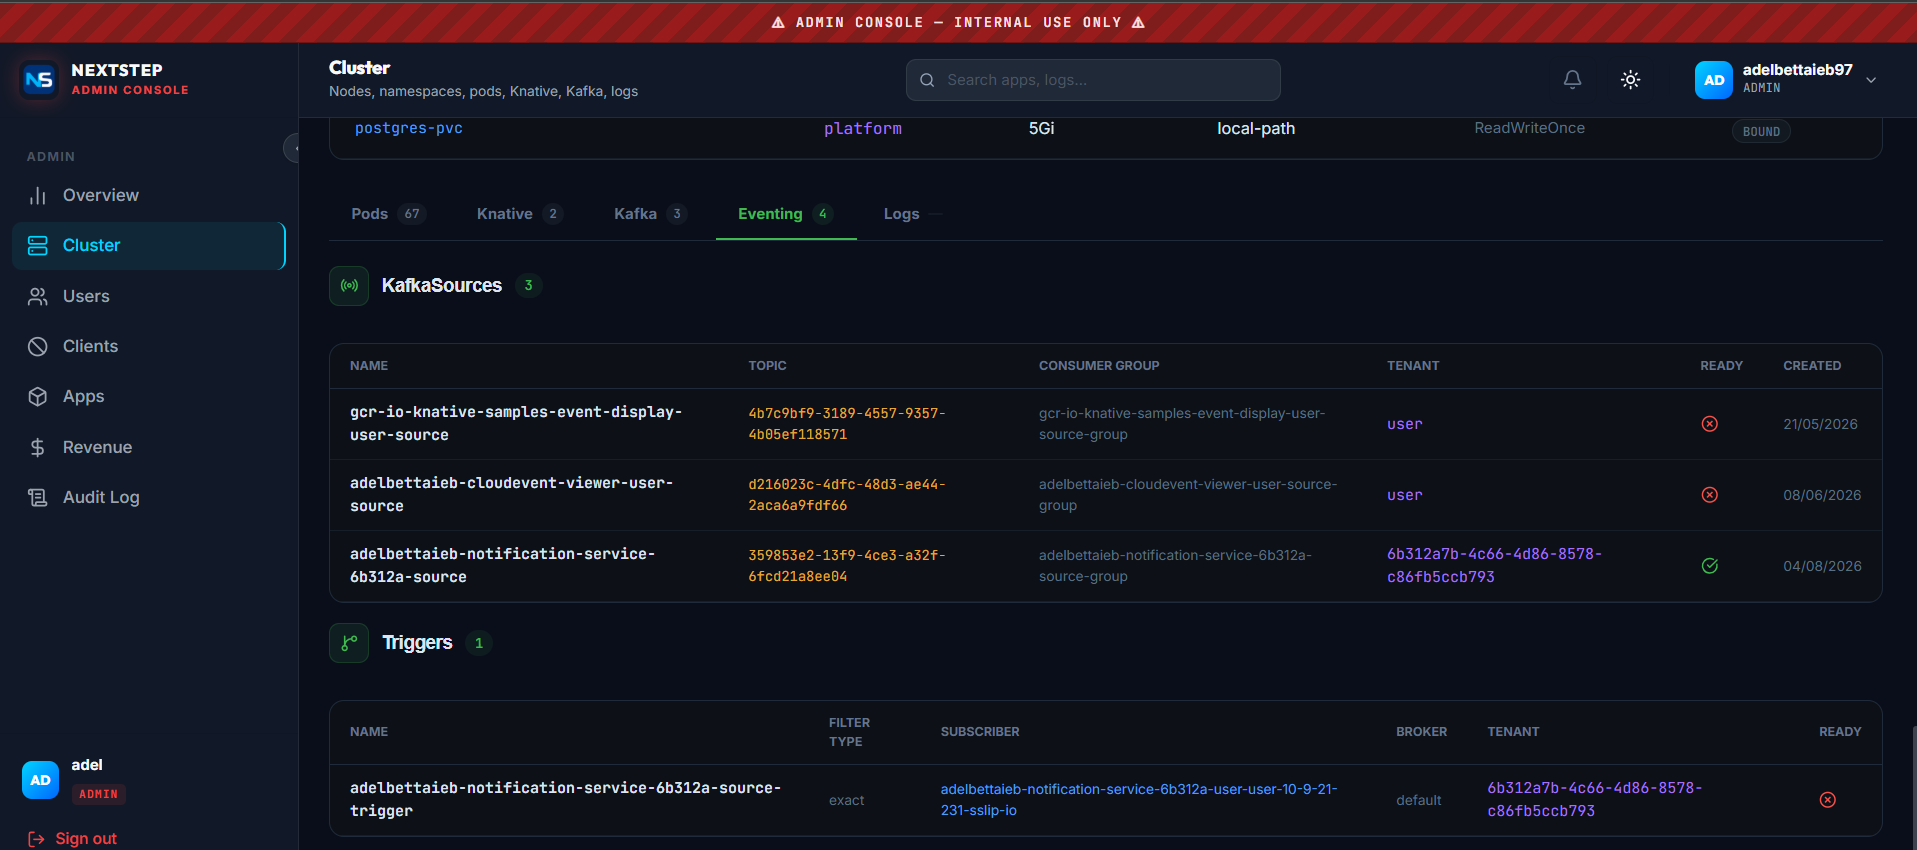
\includegraphics[width=0.9\textwidth]{image/ue administrateur des sujets, sources et déclencheurs.png}
    \caption{Vue administrateur des sujets, sources et déclencheurs}
    \label{fig:capture-admineventing}
\end{figure}

Le déploiement d'une application (Sprint 4) peut également câbler automatiquement un déclencheur, dans le même mouvement que la création de l'application, si le formulaire de déploiement renseigne un sujet Kafka.

\subsection{Conclusion}

Ce sprint relie Kafka et Knative Eventing en un service de messagerie événementielle complet et exposé au client : sujets, sources et déclencheurs sont créés, consultés et supprimés depuis le portail, avec une supervision globale côté ADMIN. La plateforme dispose désormais des trois grandes fonctions applicatives — accès, applications, événements — sur lesquelles s'appuie l'observabilité, objet du sprint suivant.

\clearpage
\section{Sprint 6 : Gestion de l'observabilité applicative}

\subsection{Introduction}

Ce sprint dote le portail client des capacités d'observation de ses propres applications : journaux de déploiement et applicatifs en temps réel, métriques de charge. La supervision de l'ensemble du cluster, réservée à l'ADMIN, est un domaine distinct traité au Sprint 9.

\subsection{Sprint Backlog}

Le tableau~\ref{tab:sb-sprint6} présente le backlog détaillé du Sprint 6, obtenu en décomposant chaque User Story retenue en tâches techniques.

\needspace{0.9\textheight}
{
\setlength{\LTleft}{-1.5cm}
\setlength{\LTright}{-1.5cm}
\setlength{\tabcolsep}{8pt}
\renewcommand{\arraystretch}{1.9}
\begin{longtable}{|p{6.6cm}|>{\raggedright\arraybackslash}p{8.1cm}|>{\centering\arraybackslash}p{2.3cm}|}
\hline
User Story & Tâches & Estimation \\
\hline
\endfirsthead
\hline
User Story & Tâches & Estimation \\
\hline
\endhead
\hline
\endfoot

\caption{Backlog du Sprint 6}
\label{tab:sb-sprint6}
\endlastfoot

\multirow{3}{6.6cm}{\centering En tant que CLIENT\_ADMIN, je veux consulter les journaux de déploiement de mes applications afin de diagnostiquer un problème.}
& Développer la consultation des journaux de déploiement. & 1 \\ \cline{2-3}
& Développer le filtrage par niveau. & 1 \\ \cline{2-3}
& Développer la page de consultation des journaux. & 1 \\ \hline

\multirow{2}{6.6cm}{\centering En tant que CLIENT\_ADMIN, je veux suivre les journaux applicatifs en temps réel afin d'observer le comportement de mon application en direct.}
& Développer le flux temps réel des journaux de déploiement. & 1 \\ \cline{2-3}
& Développer le flux temps réel des journaux bruts du conteneur. & 1 \\ \hline

\multirow{3}{6.6cm}{\centering En tant que CLIENT\_ADMIN, je veux consulter les métriques de mes applications afin d'évaluer leur charge et leurs performances.}
& Développer les métriques par application. & 1 \\ \cline{2-3}
& Développer le flux temps réel des métriques. & 1 \\ \cline{2-3}
& Développer la page de monitoring. & 1 \\ \hline

\multirow{2}{6.6cm}{\centering En tant qu'ADMIN, je veux consulter les journaux de déploiement de tous les locataires afin de superviser la plateforme.}
& Développer la vue administrateur des journaux. & 1 \\ \cline{2-3}
& Tester l'accès transversal aux journaux. & 1 \\ \hline

\end{longtable}
}

\subsection{Diagramme de cas d'utilisation du Sprint 6}

Le diagramme réunit CLIENT\_ADMIN et MEMBER (sous permission \texttt{VIEW\_LOGS}/\texttt{VIEW\_MONITORING}) et ADMIN, avec l'ensemble des fonctionnalités du sprint.

\begin{figure}[H]
 \centering
    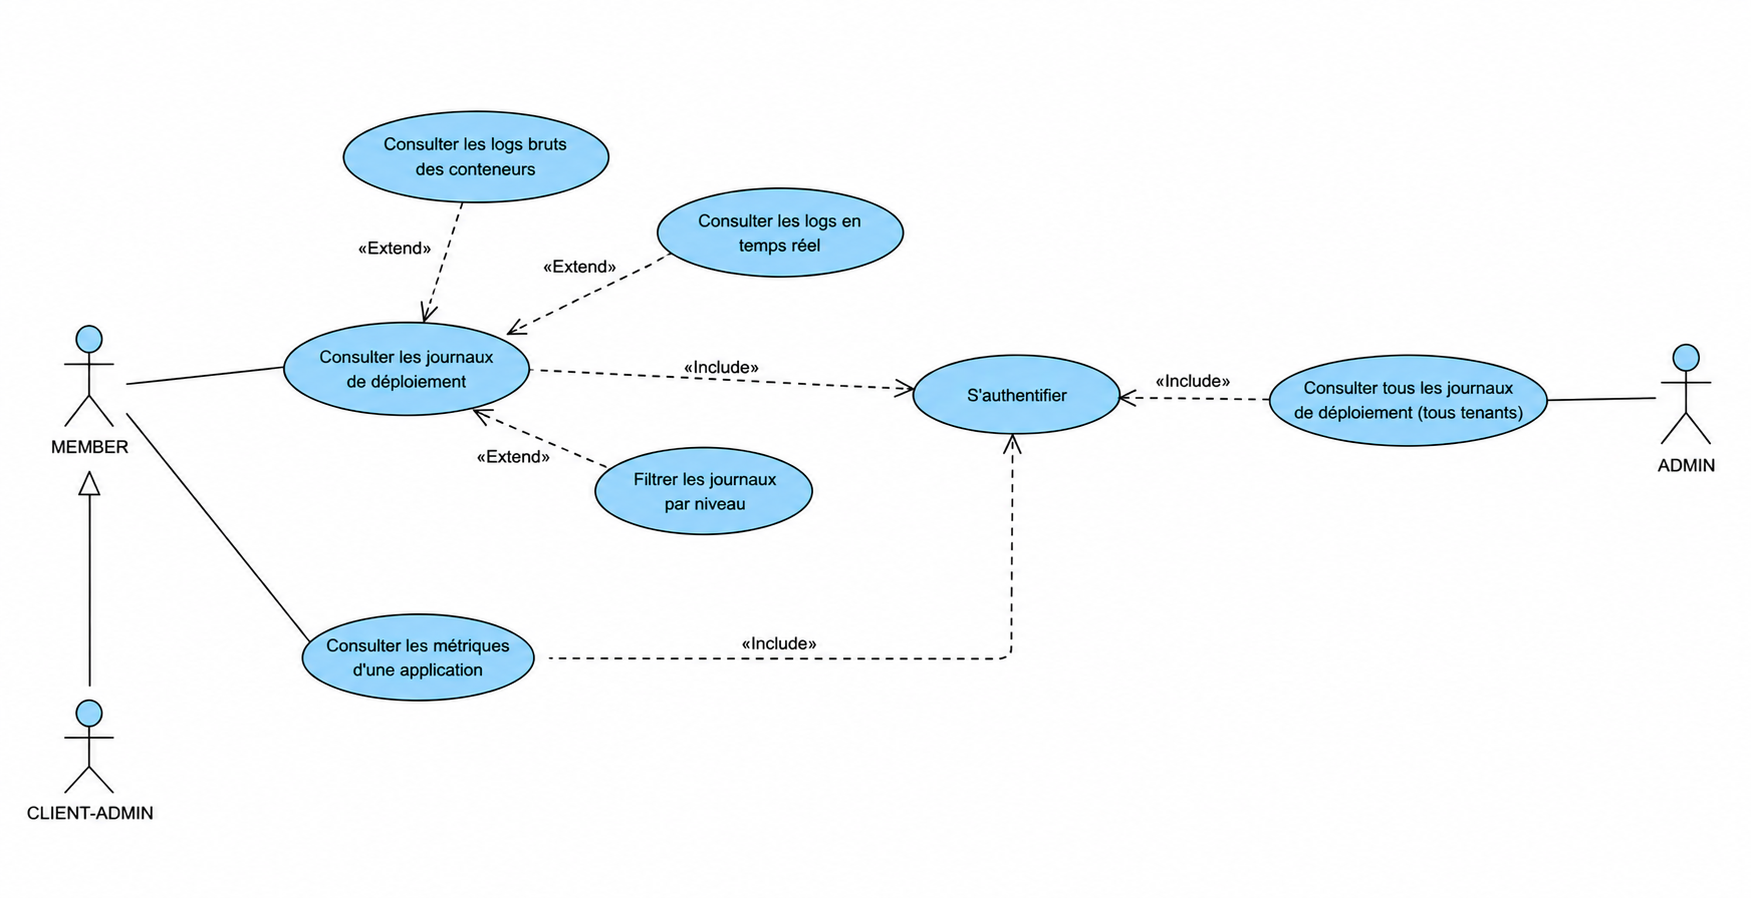
\includegraphics[width=\textwidth]{image/uc-sprint6.png}
    \caption{Diagramme de cas d'utilisation du Sprint 6 — Gestion de l'observabilité applicative}
    \label{fig:uc-sprint6}
\end{figure}

\subsection{Services Web}

\needspace{5cm}
\begin{longtable}{|p{6cm}|p{9.3cm}|}
\hline
Service Web & Description \\
\hline
\endfirsthead
\hline
Service Web & Description \\
\hline
\endhead
\hline
\endfoot
\endlastfoot
\texttt{GET /api/logs/apps/\{id\}} & Journaux de déploiement d'une application, filtrables par niveau. \\ \hline
\texttt{GET /api/logs/me} & Ses propres journaux. \\ \hline
\texttt{GET /api/logs/stream} (SSE) & Flux temps réel des journaux de déploiement. \\ \hline
\texttt{GET /api/logs/apps/\{id\}/pod-logs/stream} (SSE) & Flux temps réel des journaux bruts du conteneur. \\ \hline
\texttt{GET /api/metrics/apps/\{id\}} & Métriques d'une application (requêtes/s, latence, CPU, mémoire). \\ \hline
\texttt{GET /api/metrics/apps/\{id\}/stream} (SSE) & Flux temps réel des métriques d'une application. \\ \hline
\texttt{GET /api/admin/logs} & Journaux de déploiement de tous les locataires (ADMIN). \\ \hline
\end{longtable}

\subsection{Conception}

Deux fonctionnalités sont détaillées : la consultation des journaux en temps réel, dont la mise en œuvre a nécessité une correction de sécurité notable ; la consultation des métriques, appuyée sur Prometheus.

\subsubsection{Cas d'utilisation : « Consulter les journaux en temps réel »}

\subsubsection*{Description textuelle}

\renewcommand{\arraystretch}{1.5}
\begin{longtable}{|p{4cm}|p{11cm}|}
\hline
Nom & Consulter les journaux d'une application en temps réel \\
\hline
Acteur & CLIENT\_ADMIN, MEMBER (avec permission de consultation des journaux) \\
\hline
Pré-condition & L'application appartient au compte de l'utilisateur (ou de son CLIENT\_ADMIN) \\
\hline
Scénario nominal & 1. L'utilisateur ouvre la page de journaux de son application. 2. Le portail établit une connexion en flux continu vers le backend. 3. Le backend récupère les journaux du conteneur applicatif du pod concerné et les diffuse en temps réel. 4. L'utilisateur visualise les journaux au fil de leur émission. \\
\hline
Post-condition & L'utilisateur dispose d'une vue à jour de l'activité de son application. \\
\hline
\caption{Description textuelle du cas d'utilisation « Consulter les journaux en temps réel »}
\label{tab:uc-logs}
\end{longtable}

\subsubsection*{Diagramme de séquence}

\begin{figure}[H]
 \centering
    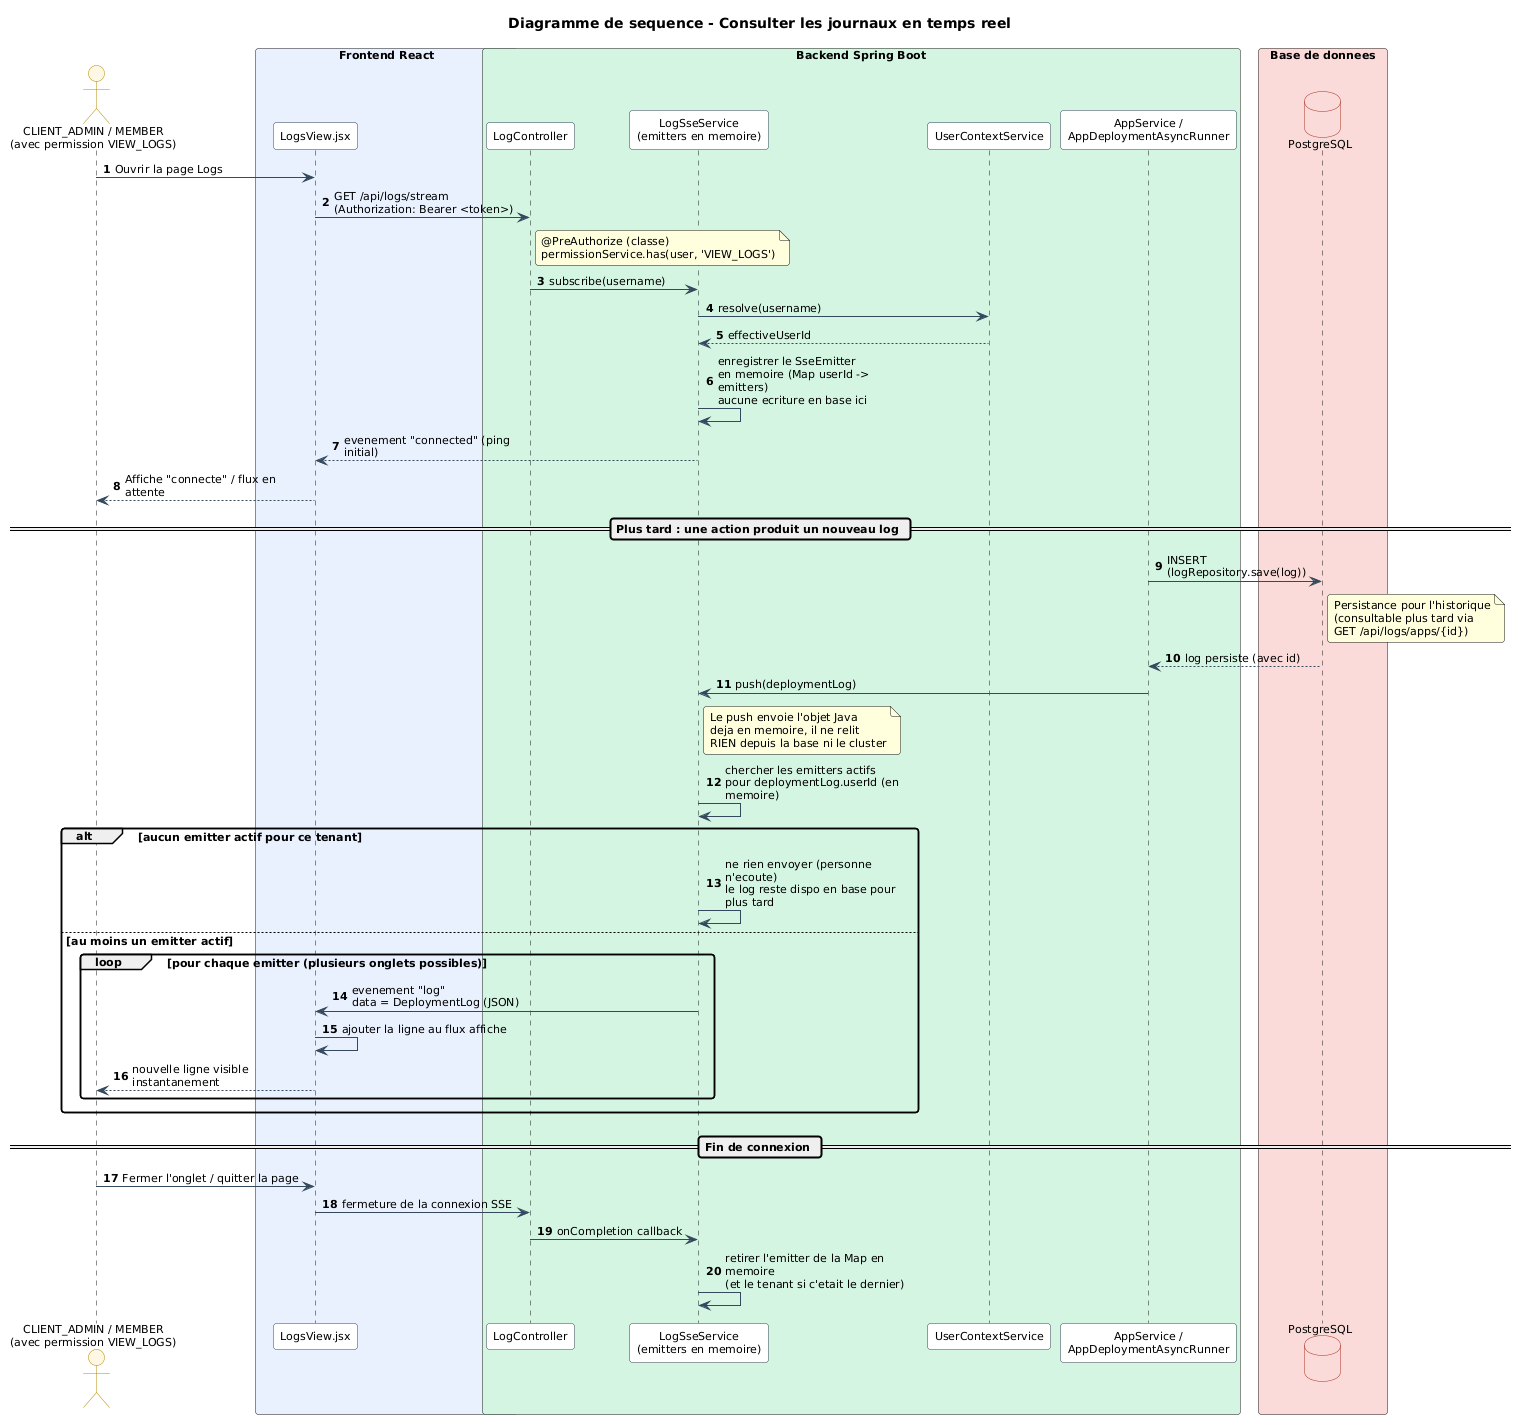
\includegraphics[width=\textwidth,height=0.85\textheight,keepaspectratio]{image/seq-logs.png}
    \caption{Diagramme de séquence — Consulter les journaux en temps réel}
    \label{fig:seq-logs}
\end{figure}



\subsection{Réalisation du Sprint 6}

Fonctionnalité : Consulter les journaux de déploiement. La page de journaux affiche, pour une application donnée, ses journaux de déploiement filtrables par niveau.

\begin{figure}[H]
 \centering
    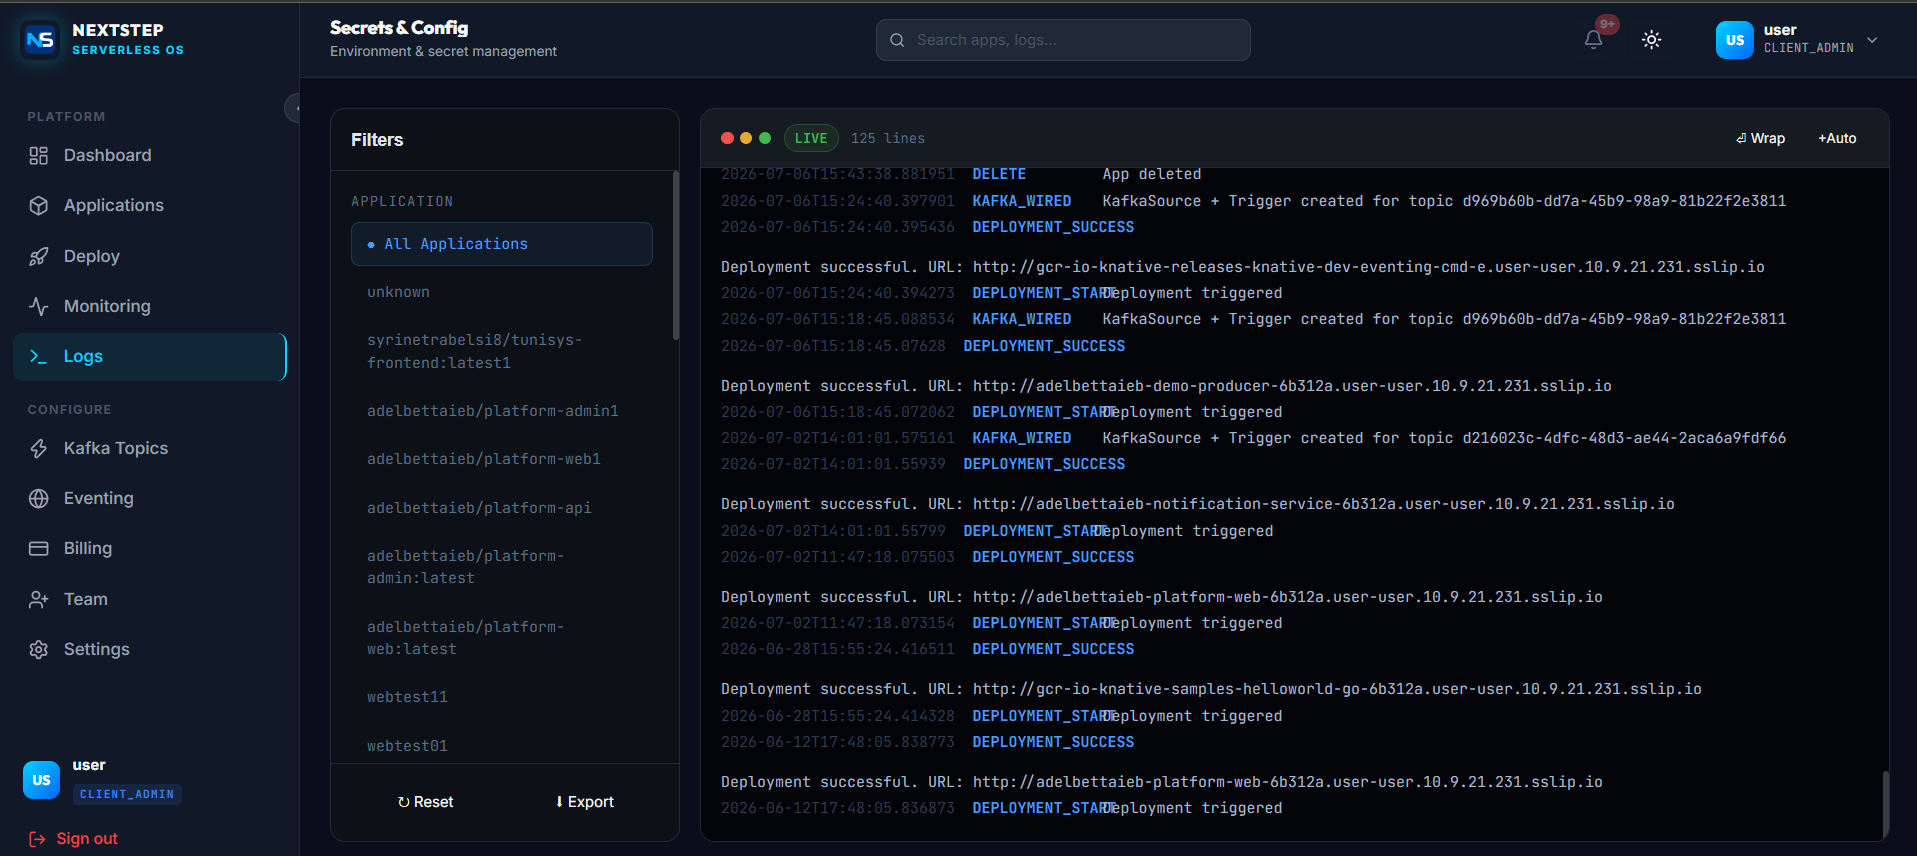
\includegraphics[width=0.9\textwidth]{image/Interface de consultation des journaux de déploiemen.png}
    \caption{Interface de consultation des journaux de déploiement}
    \label{fig:capture-deploylogs}
\end{figure}

Fonctionnalité : Suivre les journaux en temps réel. La même page diffuse en continu les journaux applicatifs bruts du conteneur.

\begin{figure}[H]
 \centering
    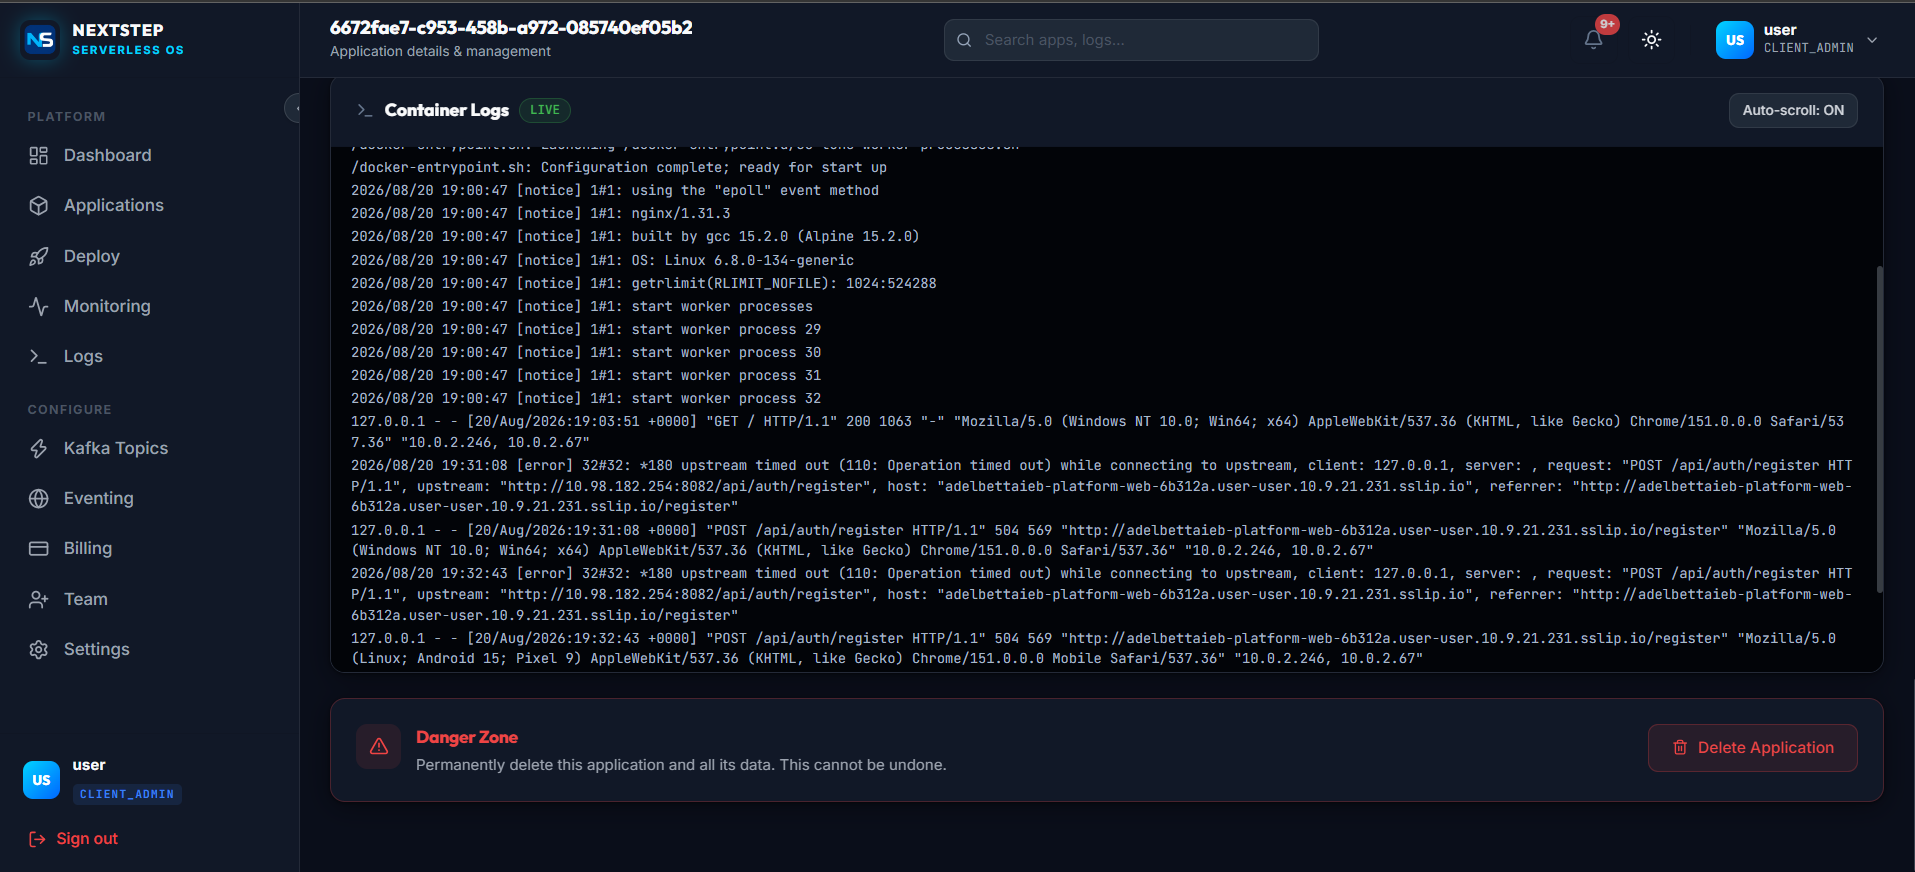
\includegraphics[width=0.9\textwidth]{image/Flux temps réel des journaux applicatifs.png}
    \caption{Flux temps réel des journaux applicatifs}
    \label{fig:capture-livelogs}
\end{figure}



Fonctionnalité : Consulter les journaux de tous les locataires (ADMIN). L'ADMIN consulte, depuis la console d'administration, les journaux de déploiement de l'ensemble des clients.

\begin{figure}[H]
 \centering
    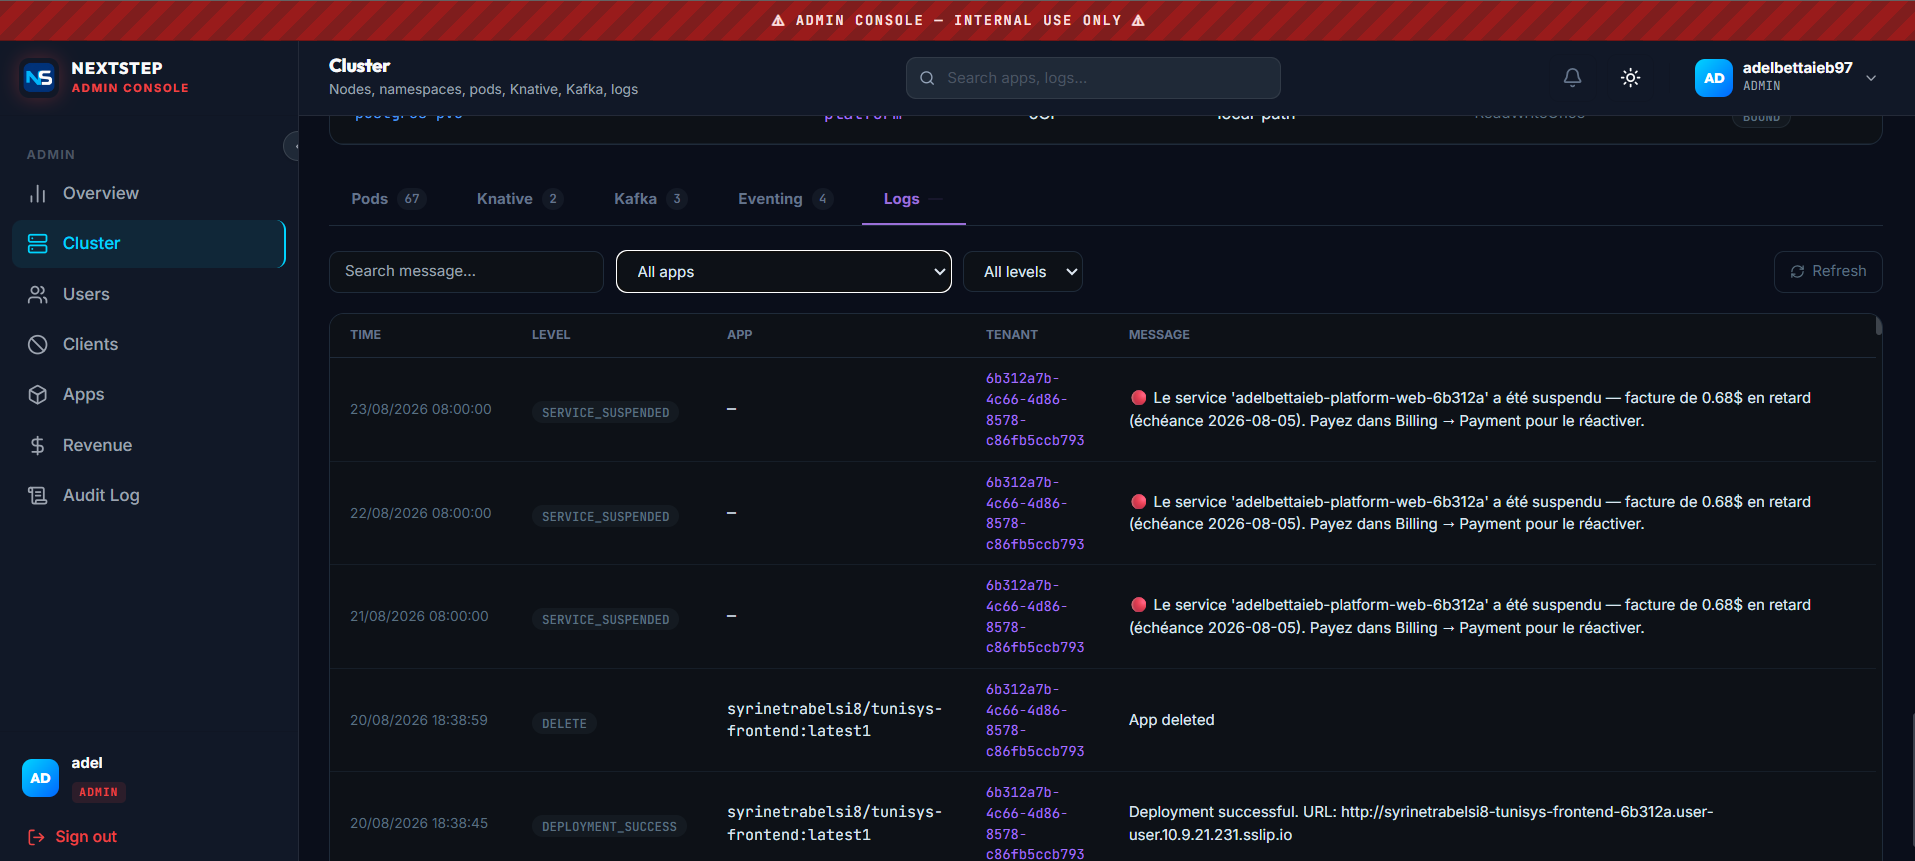
\includegraphics[width=0.9\textwidth]{image/Vue administrateur des journau.png}
    \caption{Vue administrateur des journaux}
    \label{fig:capture-adminlogs}
\end{figure}

\subsection{Conclusion}

Ce sprint livre l'observabilité applicative côté client : journaux et métriques, en différé comme en temps réel, avec une vue transversale côté ADMIN. La Release 1 est désormais complète : accès, applications, messagerie événementielle et observabilité constituent le cœur applicatif de la plateforme.

\section{Conclusion}

La Release 1 a transformé le socle technique de la Release 0 en un cœur applicatif cohérent, organisé par domaine de gestion plutôt que par brique livrée : accès et identité, cycle de vie des applications, messagerie événementielle, observabilité. Chaque sprint réunit tous les acteurs concernés par son domaine, du visiteur à l'ADMIN, et livre conjointement la brique backend et l'écran du portail qui l'expose. Plusieurs anomalies de cohérence et de sécurité identifiées au fil de ces sprints sont assumées comme limites du projet.


\chapter{Release 2 : Exploitation et commercialisation}

\section{Introduction}

La Release 1 a livré le cœur applicatif de la plateforme, accessible au CLIENT\_ADMIN et aux MEMBER de son équipe. Cette release complète la plateforme du point de vue de son exploitant, l'équipe de NextStep IT, et d'un besoin transversal aux deux profils : la facturation. Elle regroupe trois sprints : le Sprint 7, qui livre la facturation à l'usage et les paiements ; le Sprint 8, qui livre la gestion des comptes clients, de leurs quotas et l'audit des actions administratives ; le Sprint 9, qui livre la supervision du cluster et le statut public de la plateforme.

\section{Sprint 7 : Gestion de la facturation et des paiements}

\subsection{Introduction}

Ce sprint facture l'usage réel des applications déployées sur la plateforme et permet son règlement en ligne. Il s'adresse au CLIENT\_ADMIN (et au MEMBER autorisé) pour la consultation et le paiement, et à l'ADMIN pour le pilotage global.

\subsection{Sprint Backlog}
Le tableau~\ref{tab:sb-sprint7} présente le backlog détaillé du Sprint 7, obtenu en décomposant chaque User Story retenue en tâches techniques.

{
\setlength{\LTleft}{-1.5cm}
\setlength{\LTright}{-1.5cm}
\setlength{\tabcolsep}{8pt}
\renewcommand{\arraystretch}{1.9}
\begin{longtable}{|p{6.6cm}|>{\raggedright\arraybackslash}p{8.1cm}|>{\centering\arraybackslash}p{2.3cm}|}
\hline
User Story & Tâches & Estimation \\
\hline
\endfirsthead

\multicolumn{3}{l}{\small\itshape (suite du tableau~\ref{tab:sb-sprint7})}\\
\hline
User Story & Tâches & Estimation \\
\hline
\endhead

\hline
\multicolumn{3}{r}{\small\itshape (suite page suivante)}\\
\endfoot

\hline
\caption{Backlog du Sprint 7}
\label{tab:sb-sprint7}
\endlastfoot

\multirow{3}{6.6cm}{\centering En tant que CLIENT\_ADMIN ou MEMBER, je veux consulter mon historique d'usage et de facturation afin de suivre mes dépenses.}
& Développer le calcul périodique de l'usage. & 2 \\* \cline{2-3}
& Développer la consultation de sa facturation. & 1 \\* \cline{2-3}
& Développer la page de facturation du portail. & 1 \\ \hline

\multirow{7}{6.6cm}{\centering En tant que CLIENT\_ADMIN ou MEMBER, je veux gérer mes moyens de paiement, régler mes factures et consulter mes transactions afin de rester en règle.}
& Intégrer le prestataire de paiement. & 3 \\* \cline{2-3}
& Développer l'enregistrement d'un moyen de paiement. & 2 \\* \cline{2-3}
& Développer la suppression d'un moyen de paiement. & 1 \\* \cline{2-3}
& Développer la liste de ses factures. & 1 \\* \cline{2-3}
& Développer le paiement d'une facture. & 3 \\* \cline{2-3}
& Développer la consultation de ses transactions. & 1 \\* \cline{2-3}
& Tester le paiement. & 2 \\ \hline

\multirow{2}{6.6cm}{\centering En tant que CLIENT\_ADMIN ou MEMBER, je veux exporter un rapport de facturation afin de le transmettre à ma comptabilité.}
& Développer l'export du rapport de facturation. & 2 \\ \cline{2-3}
& Tester l'export du rapport de facturation. & 1 \\ \hline

\multirow{4}{6.6cm}{\centering En tant qu'ADMIN, je veux consulter la facturation de tous les clients, les factures impayées, et générer les factures mensuelles afin de piloter la facturation globale.}
& Développer la vue de facturation globale. & 2 \\* \cline{2-3}
& Développer la consultation des factures impayées. & 1 \\* \cline{2-3}
& Développer la génération mensuelle des factures. & 2 \\* \cline{2-3}
& Développer le déclenchement manuel d'un instantané d'usage. & 1 \\ \hline

\multirow{2}{6.6cm}{\centering En tant qu'ADMIN, je veux suspendre manuellement un client en situation d'impayé afin de limiter les pertes.}
& Développer la suspension manuelle pour non-paiement. & 2 \\* \cline{2-3}
& Tester ce mécanisme. & 1 \\ \hline
\end{longtable}
}
% \subsection{Sprint Backlog}

% Le tableau~\ref{tab:sb-sprint7} présente le backlog détaillé du Sprint 7, obtenu en décomposant chaque User Story retenue en tâches techniques.

% \needspace{0.75\textheight}
% {
% \setlength{\LTleft}{-1.5cm}
% \setlength{\LTright}{-1.5cm}
% \setlength{\tabcolsep}{8pt}
% \renewcommand{\arraystretch}{1.9}
% \begin{longtable}{|p{6.6cm}|>{\raggedright\arraybackslash}p{8.1cm}|>{\centering\arraybackslash}p{2.3cm}|}
% \hline
% User Story & Tâches & Estimation \\
% \hline
% \endfirsthead
% \hline
% User Story & Tâches & Estimation \\
% \hline
% \endhead
% \endfoot
% \hline

% \caption{Backlog du Sprint 7}
% \label{tab:sb-sprint7}
% \endlastfoot

% \multirow{3}{6.6cm}{\centering En tant que CLIENT\_ADMIN ou MEMBER, je veux consulter mon historique d'usage et de facturation afin de suivre mes dépenses.}
% & Développer le calcul périodique de l'usage. & 1 \\ \cline{2-3}
% & Développer la consultation de sa facturation. & 1 \\ \cline{2-3}
% & Développer la page de facturation du portail. & 1 \\ \hline

% \multirow{7}{6.6cm}{\centering En tant que CLIENT\_ADMIN ou MEMBER, je veux gérer mes moyens de paiement, régler mes factures et consulter mes transactions afin de rester en règle.}
% & Intégrer le prestataire de paiement. & 1 \\ \cline{2-3}
% & Développer l'enregistrement d'un moyen de paiement. & 1 \\ \cline{2-3}
% & Développer la suppression d'un moyen de paiement. & 1 \\ \cline{2-3}
% & Développer la liste de ses factures. & 1 \\ \cline{2-3}
% & Développer le paiement d'une facture. & 1 \\ \cline{2-3}
% & Développer la consultation de ses transactions. & 1 \\ \cline{2-3}
% & Tester le paiement. & 1 \\ \hline

% \multirow{1}{6.6cm}{\centering En tant que CLIENT\_ADMIN ou MEMBER, je veux exporter un rapport de facturation afin de le transmettre à ma comptabilité.}
% & Développer l'export du rapport de facturation. & 1 \\ \hline

% \multirow{4}{6.6cm}{\centering En tant qu'ADMIN, je veux consulter la facturation de tous les clients, les factures impayées, et générer les factures mensuelles afin de piloter la facturation globale.}
% & Développer la vue de facturation globale. & 1 \\ \cline{2-3}
% & Développer la consultation des factures impayées. & 1 \\ \cline{2-3}
% & Développer la génération mensuelle des factures. & 1 \\ \cline{2-3}
% & Développer le déclenchement manuel d'un instantané d'usage. & 1 \\ \hline

% \multirow{2}{6.6cm}{\centering En tant qu'ADMIN, je veux suspendre manuellement un client en situation d'impayé afin de limiter les pertes.}
% & Développer la suspension manuelle pour non-paiement. & 1 \\ \cline{2-3}
% & Tester ce mécanisme. & 1 \\ \hline

% \end{longtable}
% }

\subsection{Diagramme de cas d'utilisation du Sprint 7}

Le diagramme réunit CLIENT\_ADMIN et MEMBER (sous permission \texttt{VIEW\_BILLING}/\texttt{EXPORT\_BILLING}), ADMIN, et le prestataire de paiement (acteur externe, notification par webhook), avec l'ensemble des fonctionnalités du sprint.

\begin{figure}[H]
 \centering
    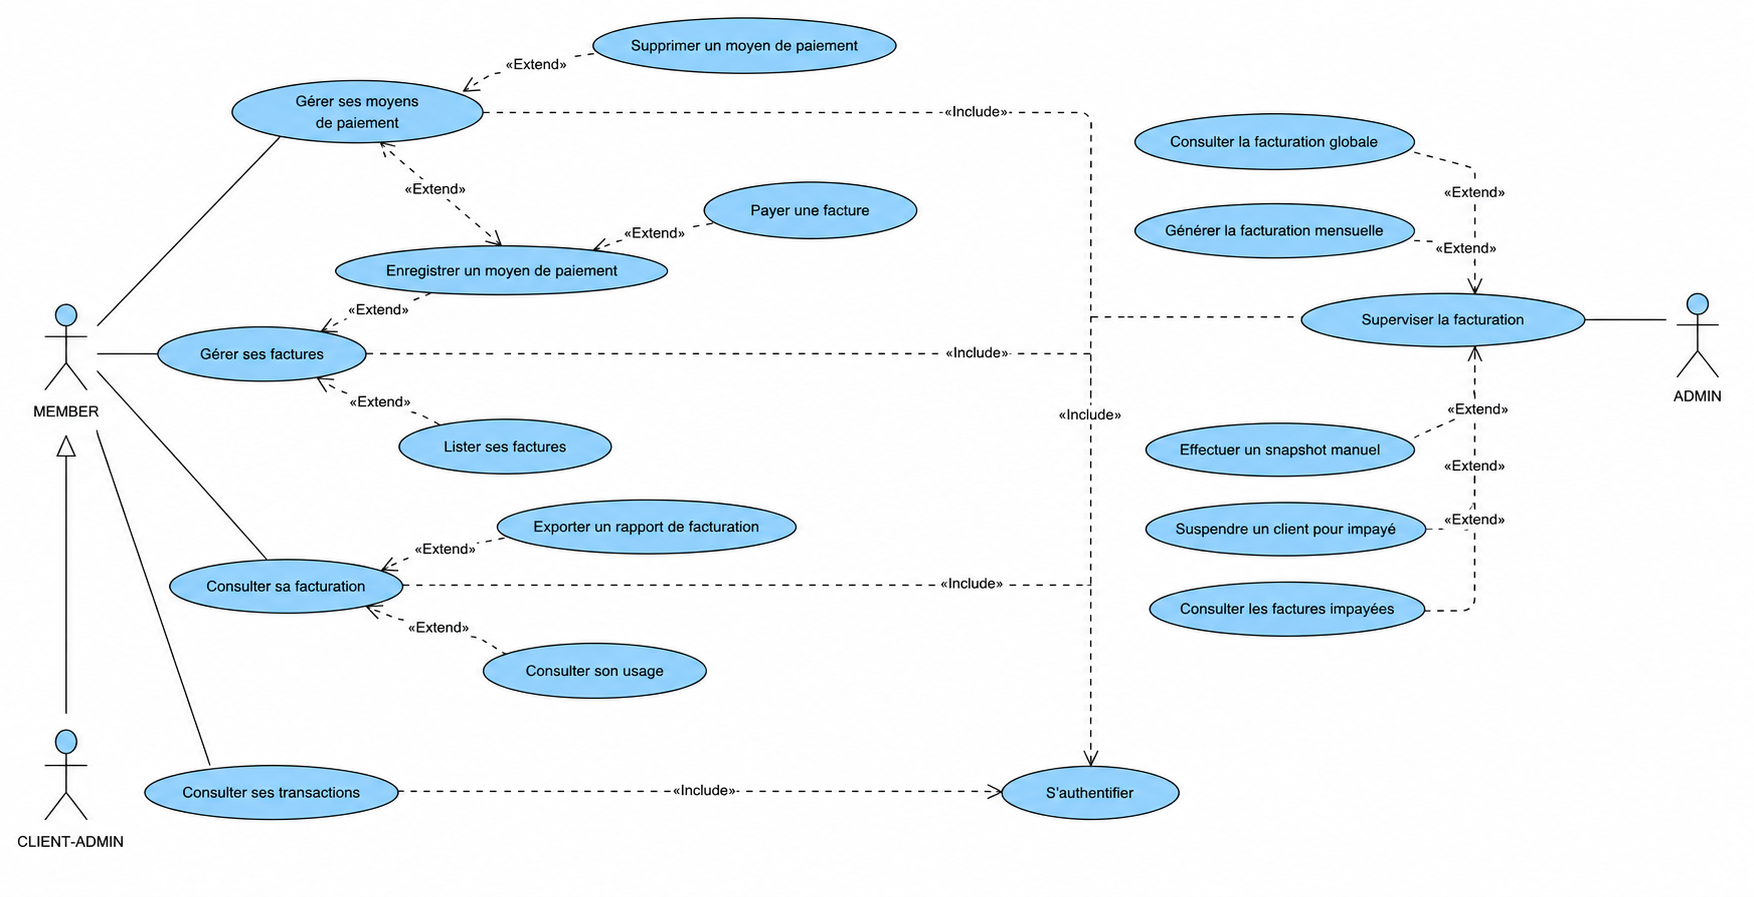
\includegraphics[width=\textwidth]{image/usescase7.png}
    \caption{Diagramme de cas d'utilisation du Sprint 7 — Gestion de la facturation et des paiements}
    \label{fig:uc-sprint7}
\end{figure}
\subsection{Services Web}
{\setlength{\tabcolsep}{8pt}
\begin{longtable}{|p{5.8cm}|p{8.4cm}|}
\hline
Service Web & Description \\
\hline
\endfirsthead
\hline
Service Web & Description \\
\hline
\endhead
\endfoot
\hline
\endlastfoot
\texttt{GET\slash api\slash billing\slash me} & Consulter sa facturation. \\ \hline
\texttt{GET\slash api\slash billing\slash export} & Exporter un rapport de facturation. \\ \hline
\texttt{GET\slash api\slash billing\slash admin} & Facturation globale, tous clients confondus (ADMIN). \\ \hline
\texttt{POST\slash api\slash billing\slash admin\slash snapshot} & Déclencher un instantané d'usage (ADMIN). \\ \hline
\texttt{GET\slash api\slash invoices} & Lister ses factures. \\ \hline
\texttt{POST\slash api\slash invoices\slash\{id\}\slash pay} & Payer une facture. \\ \hline
\texttt{GET\slash api\slash invoices\slash admin\slash overdue} & Factures impayées (ADMIN). \\ \hline
\texttt{POST\slash api\slash invoices\slash generate} & Générer les factures mensuelles (ADMIN). \\ \hline
\texttt{POST\slash api\slash invoices\slash apps\slash\{appId\}\slash suspend} & Suspendre une application pour impayé (ADMIN). \\ \hline
\texttt{GET\slash api\slash payment\slash config} & Configuration publique du prestataire de paiement. \\ \hline
\texttt{POST\slash api\slash payment\slash setup-intent} & Enregistrer un moyen de paiement. \\ \hline
\texttt{GET\slash api\slash payment\slash methods} & Lister ses moyens de paiement. \\ \hline
\texttt{DELETE\slash api\slash payment\slash methods\slash\{id\}} & Supprimer un moyen de paiement. \\ \hline
\texttt{POST\slash api\slash payment\slash pay} & Payer. \\ \hline
\texttt{GET\slash api\slash payment\slash transactions} & Historique des transactions. \\ \hline
\texttt{POST\slash api\slash payment\slash webhook} & Notification du prestataire de paiement. \\ \hline
\end{longtable}}

% \subsection{Services Web}

% \needspace{0.55\textheight}
% {\setlength{\tabcolsep}{8pt}
% \begin{longtable}{|p{5.8cm}|p{8.4cm}|}
% \hline
% Service Web & Description \\
% \hline
% \endfirsthead
% \hline
% Service Web & Description \\
% \hline
% \endhead
% \endfoot
% \hline
% \endlastfoot
% \texttt{GET /api/billing/me} & Consulter sa facturation. \\ \hline
% \texttt{GET /api/billing/export} & Exporter un rapport de facturation. \\ \hline
% \texttt{GET /api/billing/admin} & Facturation globale, tous clients confondus (ADMIN). \\ \hline
% \texttt{POST /api/billing/admin/snapshot} & Déclencher un instantané d'usage (ADMIN). \\ \hline
% \texttt{GET /api/invoices} & Lister ses factures. \\ \hline
% \texttt{POST /api/invoices/\{id\}/pay} & Payer une facture. \\ \hline
% \texttt{GET /api/invoices/admin/overdue} & Factures impayées (ADMIN). \\ \hline
% \texttt{POST /api/invoices/generate} & Générer les factures mensuelles (ADMIN). \\ \hline
% \texttt{POST /api/invoices/apps/\{appId\}/suspend} & Suspendre une application pour impayé (ADMIN). \\ \hline
% \texttt{GET /api/payment/config} & Configuration publique du prestataire de paiement. \\ \hline
% \texttt{POST /api/payment/setup-intent} & Enregistrer un moyen de paiement. \\ \hline
% \texttt{GET /api/payment/methods} & Lister ses moyens de paiement. \\ \hline
% \texttt{DELETE /api/payment/methods/\{id\}} & Supprimer un moyen de paiement. \\ \hline
% \texttt{POST /api/payment/pay} & Payer. \\ \hline
% \texttt{GET /api/payment/transactions} & Historique des transactions. \\ \hline
% \texttt{POST /api/payment/webhook} & Notification du prestataire de paiement. \\ \hline
% \end{longtable}}

\subsection{Conception}

Une fonctionnalité est détaillée : le paiement d'une facture, techniquement la plus riche puisqu'elle implique un prestataire externe.

\needspace{0.45\textheight}
\subsubsection{Cas d'utilisation : « Payer une facture »}

\subsubsection*{Description textuelle}

\renewcommand{\arraystretch}{1.5}
\begin{longtable}{|p{4cm}|p{11cm}|}
\hline
Nom & Payer une facture \\
\hline
Acteur & CLIENT\_ADMIN \\
\hline
Pré-condition & Un moyen de paiement est enregistré ; une facture est en attente de règlement \\
\hline
Scénario nominal & 1. Le CLIENT\_ADMIN sélectionne une facture en attente. 2. Le backend déclenche le règlement auprès du prestataire de paiement avec le moyen de paiement enregistré. 3. Le prestataire notifie le backend du résultat par webhook. 4. Le statut de la facture est mis à jour. \\
\hline
Post-condition & La facture est marquée réglée, ou l'échec est signalé à l'utilisateur. \\
\hline
\caption{Description textuelle du cas d'utilisation « Payer une facture »}
\label{tab:uc-pay}
\end{longtable}

\needspace{0.35\textheight}
\subsubsection*{Diagramme de séquence}

\begin{figure}[H]
 \centering
    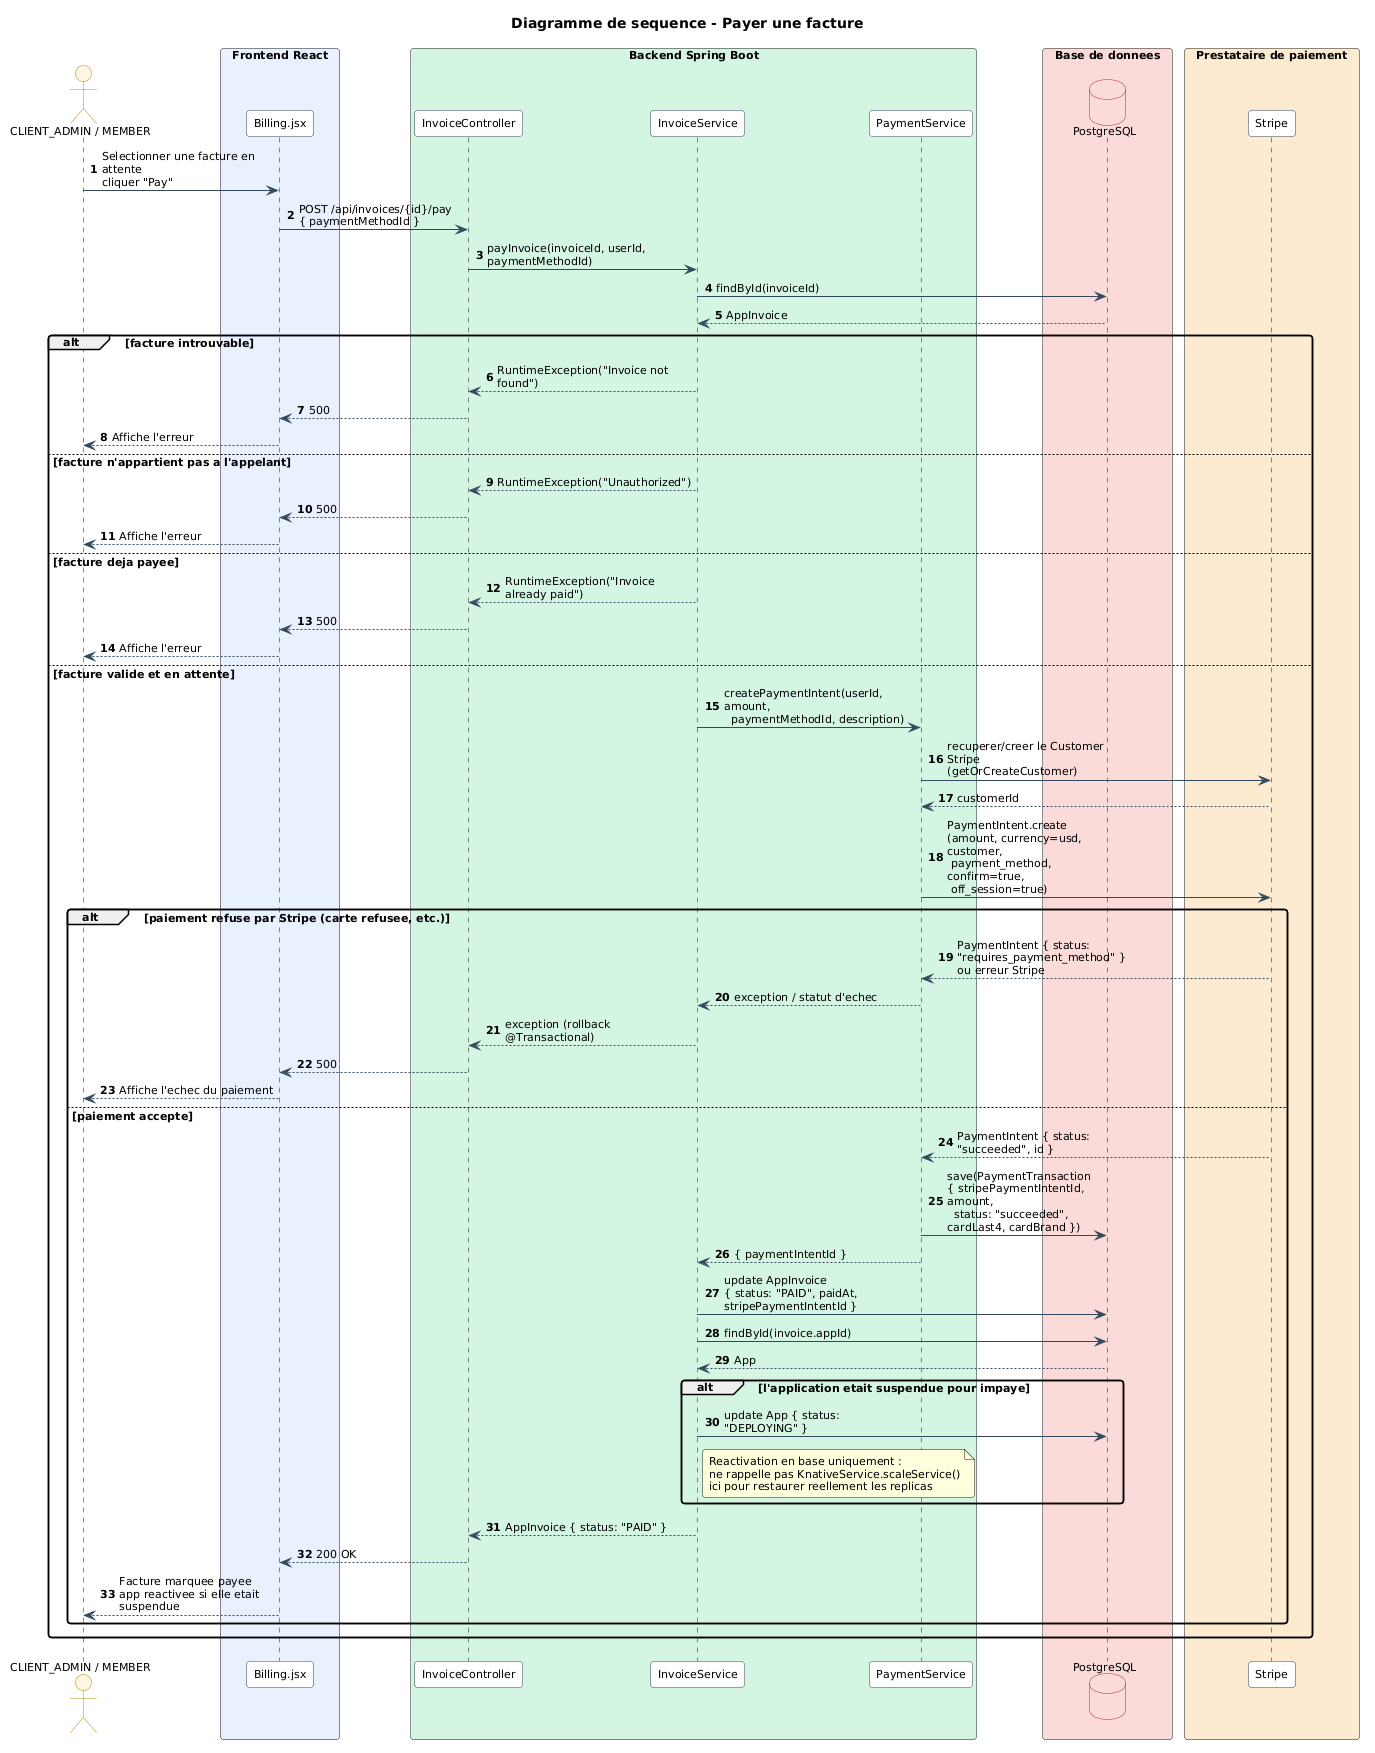
\includegraphics[width=0.9\textwidth]{image/seq-pay.png}
    \caption{Diagramme de séquence — Payer une facture}
    \label{fig:seq-pay}
\end{figure}

\subsection{Réalisation du Sprint 7}

Fonctionnalité : Consulter sa facturation, enregistrer un moyen de paiement et payer une facture. La page de facturation du portail regroupe, en un seul endroit, le coût projeté du mois en cours, l'historique des factures, les moyens de paiement enregistrés et l'historique des transactions.

\begin{figure}[H]
 \centering
    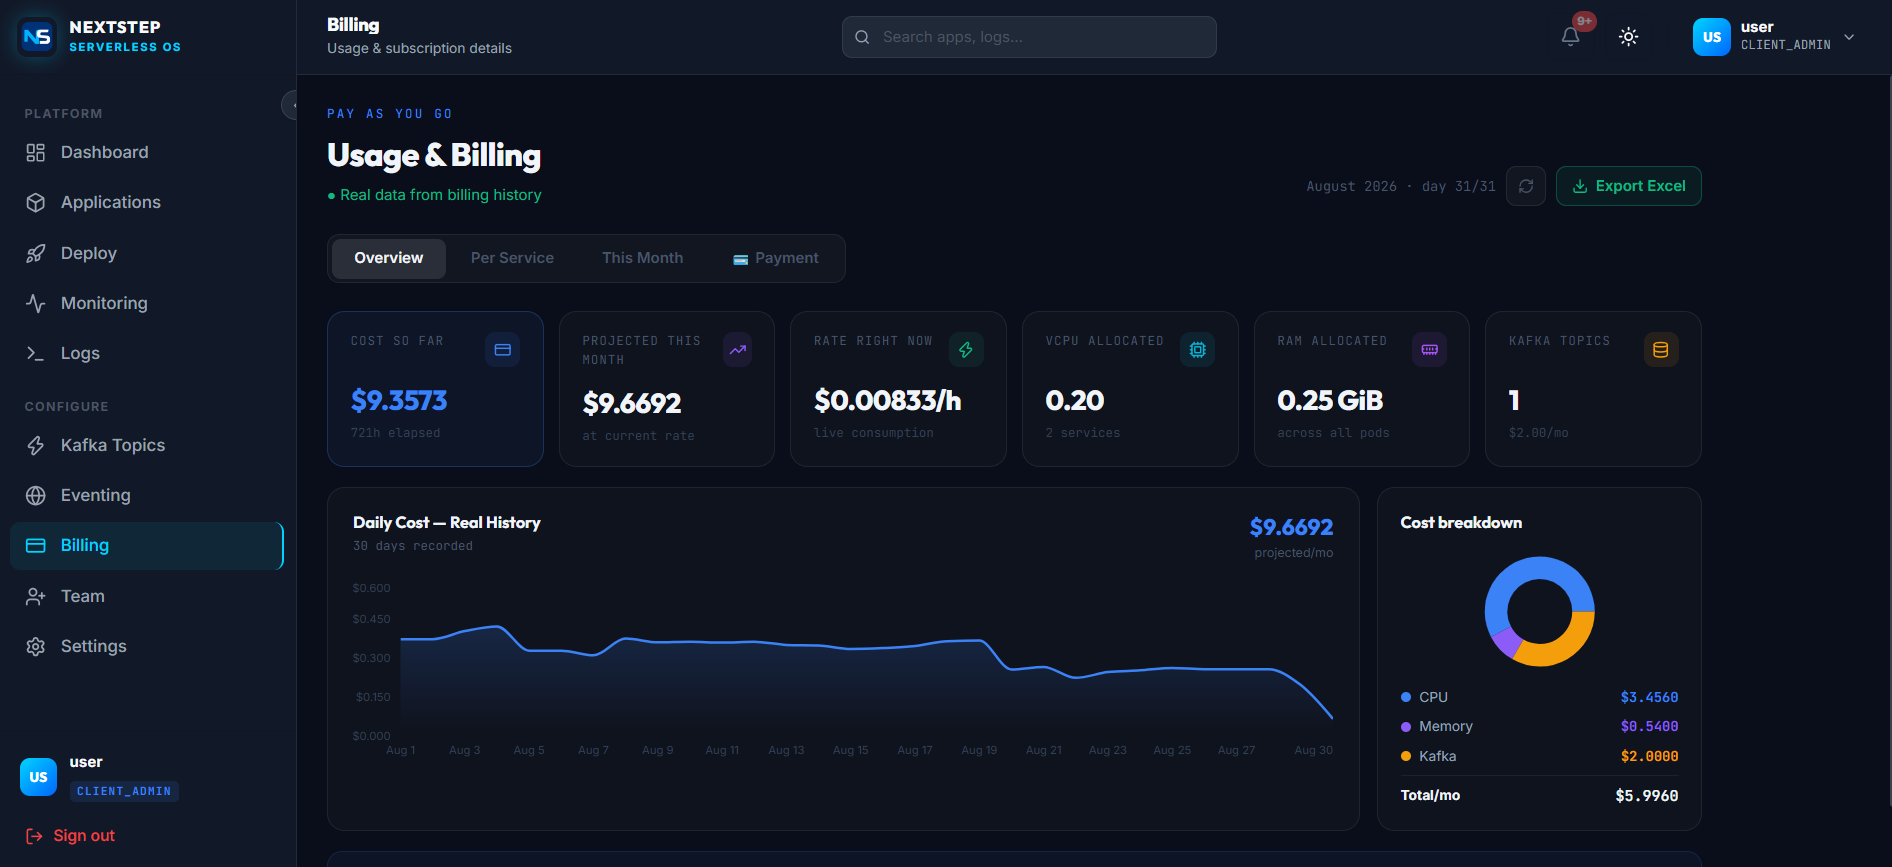
\includegraphics[width=0.9\textwidth]{image/Interface de facturation du compte client1.png}
    \caption{Interface de facturation du compte client}
    \label{fig:capture-billing}
\end{figure}

Fonctionnalité : Facturation globale et génération des factures (ADMIN). L'ADMIN consulte, depuis la console d'administration, la facturation de l'ensemble des clients et déclenche la génération des factures mensuelles.

\begin{figure}[H]
 \centering
    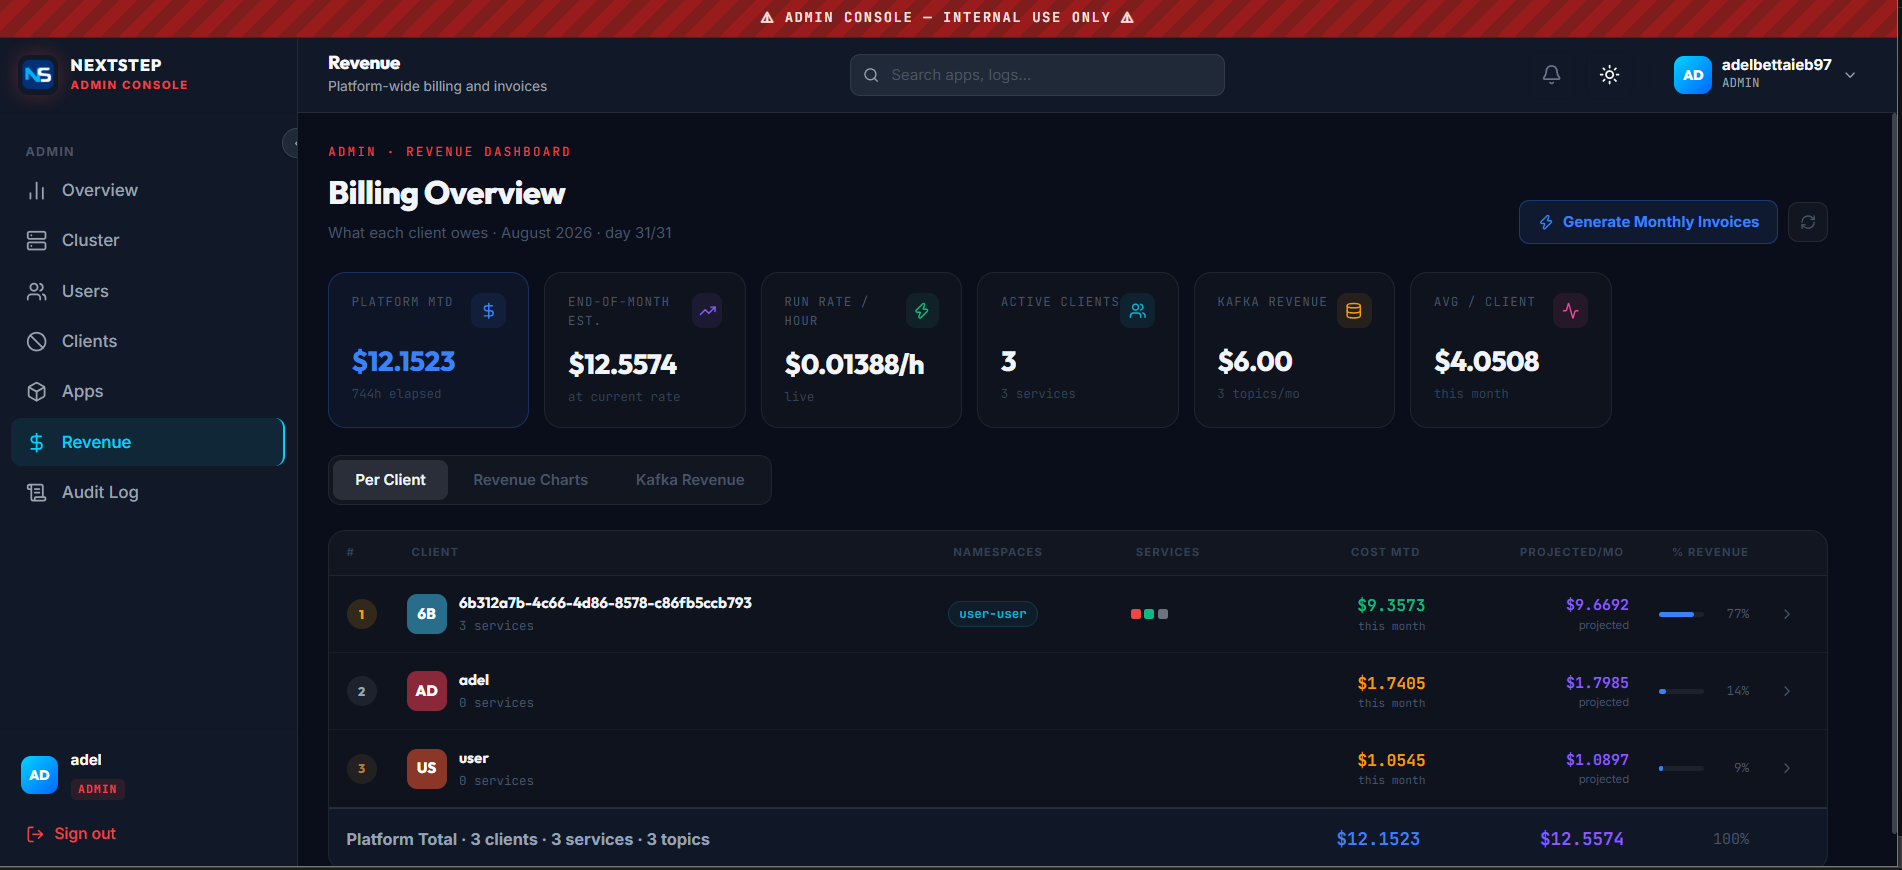
\includegraphics[width=0.9\textwidth]{image/Interface de facturation globale (console d’administration)1.png}
    \caption{Interface de facturation globale (console d'administration)}
    \label{fig:capture-adminbilling}
\end{figure}

Fonctionnalité : Payer une facture en retard (CLIENT\_ADMIN). Le client règle une facture en retard directement depuis l'onglet Payment de son portail, avec un moyen de paiement déjà enregistré.

\begin{figure}[H]
 \centering
    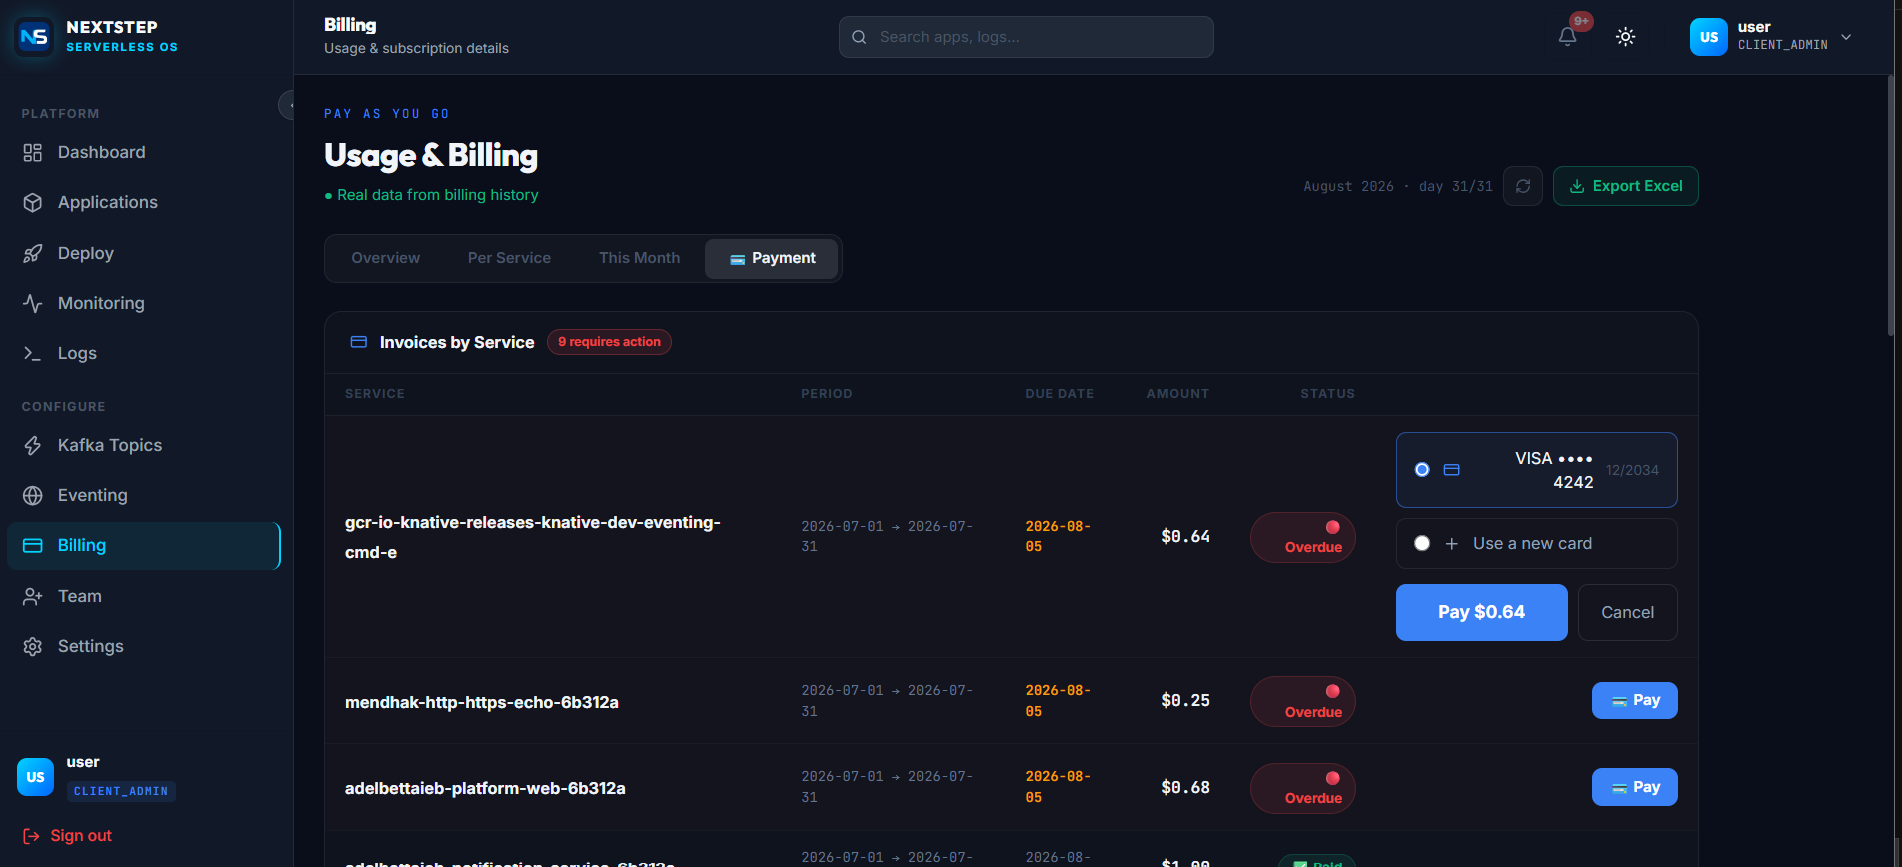
\includegraphics[width=0.9\textwidth]{image/payerune facture.png}
    \caption{Paiement d'une facture en retard par le client}
    \label{fig:capture-client-pay}
\end{figure}

\subsection{Conclusion}

Ce sprint livre la facturation à l'usage et son règlement en ligne, consultables par le client comme par l'équipe d'exploitation. Aucune limite de ressources par défaut n'est appliquée par tenant, ce qui expose le modèle à une facturation potentiellement illimitée en l'absence d'action du client ; ce point est repris au chapitre de validation.

\section{Sprint 8 : Gestion des comptes clients, des quotas et de l'audit}

\subsection{Introduction}

Ce sprint donne à l'ADMIN les moyens de gérer les comptes clients eux-mêmes : suspension, réactivation, quotas de ressources, et la traçabilité des actions administratives sensibles au travers d'un journal d'audit exportable. C'est un domaine exclusivement réservé à l'ADMIN, distinct de la gestion des utilisateurs individuels (Sprint 3).
\subsection{Sprint Backlog}
Le tableau~\ref{tab:sb-sprint8} présente le backlog détaillé du Sprint 8, obtenu en décomposant chaque User Story retenue en tâches techniques.

{
\setlength{\LTleft}{-1.5cm}
\setlength{\LTright}{-1.5cm}
\setlength{\tabcolsep}{8pt}
\renewcommand{\arraystretch}{1.9}
\begin{longtable}{|p{6.6cm}|>{\raggedright\arraybackslash}p{8.1cm}|>{\centering\arraybackslash}p{2.3cm}|}
\hline
User Story & Tâches & Estimation \\
\hline
\endfirsthead

\multicolumn{3}{l}{\small\itshape (suite du tableau~\ref{tab:sb-sprint8})}\\
\hline
User Story & Tâches & Estimation \\
\hline
\endhead

\hline
\multicolumn{3}{r}{\small\itshape (suite page suivante)}\\
\endfoot

\hline
\caption{Backlog du Sprint 8}
\label{tab:sb-sprint8}
\endlastfoot

\multirow{4}{6.6cm}{\centering En tant qu'ADMIN, je veux lister et suspendre ou réactiver un compte client afin de gérer les abus ou les impayés.}
& Développer la liste des comptes clients avec leur état. & 1 \\* \cline{2-3}
& Développer la suspension d'un compte. & 2 \\* \cline{2-3}
& Développer la réactivation d'un compte. & 1 \\* \cline{2-3}
& Tester ces actions. & 1 \\ \hline

\multirow{3}{6.6cm}{\centering En tant qu'ADMIN, je veux consulter et modifier le quota de ressources d'un client afin d'encadrer sa consommation.}
& Développer la consultation du quota. & 1 \\* \cline{2-3}
& Développer la modification du quota. & 1 \\* \cline{2-3}
& Propager le quota vers le cluster. & 2 \\ \hline

\multirow{3}{6.6cm}{\centering En tant qu'ADMIN, je veux consulter et exporter le journal d'audit des actions administratives afin de garder une traçabilité.}
& Développer l'enregistrement automatique des actions administratives. & 2 \\* \cline{2-3}
& Développer la consultation paginée et filtrable du journal. & 2 \\* \cline{2-3}
& Développer l'export CSV. & 1 \\ \hline
\end{longtable}
}

% \subsection{Sprint Backlog}

% Le tableau~\ref{tab:sb-sprint8} présente le backlog détaillé du Sprint 8, obtenu en décomposant chaque User Story retenue en tâches techniques.

% \needspace{0.75\textheight}
% {
% \setlength{\LTleft}{-1.5cm}
% \setlength{\LTright}{-1.5cm}
% \setlength{\tabcolsep}{8pt}
% \renewcommand{\arraystretch}{1.9}
% \begin{longtable}{|p{6.6cm}|>{\raggedright\arraybackslash}p{8.1cm}|>{\centering\arraybackslash}p{2.3cm}|}
% \hline
% User Story & Tâches & Estimation \\
% \hline
% \endfirsthead
% \hline
% User Story & Tâches & Estimation \\
% \hline
% \endhead
% \endfoot
% \hline

% \caption{Backlog du Sprint 8}
% \label{tab:sb-sprint8}
% \endlastfoot

% \multirow{4}{6.6cm}{\centering En tant qu'ADMIN, je veux lister et suspendre ou réactiver un compte client afin de gérer les abus ou les impayés.}
% & Développer la liste des comptes clients avec leur état. & 1 \\ \cline{2-3}
% & Développer la suspension d'un compte. & 1 \\ \cline{2-3}
% & Développer la réactivation d'un compte. & 1 \\ \cline{2-3}
% & Tester ces actions. & 1 \\ \hline

% \multirow{3}{6.6cm}{\centering En tant qu'ADMIN, je veux consulter et modifier le quota de ressources d'un client afin d'encadrer sa consommation.}
% & Développer la consultation du quota. & 1 \\ \cline{2-3}
% & Développer la modification du quota. & 1 \\ \cline{2-3}
% & Propager le quota vers le cluster. & 1 \\ \hline

% \multirow{3}{6.6cm}{\centering En tant qu'ADMIN, je veux consulter et exporter le journal d'audit des actions administratives afin de garder une traçabilité.}
% & Développer l'enregistrement automatique des actions administratives. & 1 \\ \cline{2-3}
% & Développer la consultation paginée et filtrable du journal. & 1 \\ \cline{2-3}
% & Développer l'export CSV. & 1 \\ \hline

% \end{longtable}
% }

\subsection{Diagramme de cas d'utilisation du Sprint 8}

Acteur unique : ADMIN. Le diagramme réunit l'ensemble des fonctionnalités du sprint : gestion des comptes clients, gestion des quotas, consultation et export du journal d'audit.

\begin{figure}[H]
 \centering
    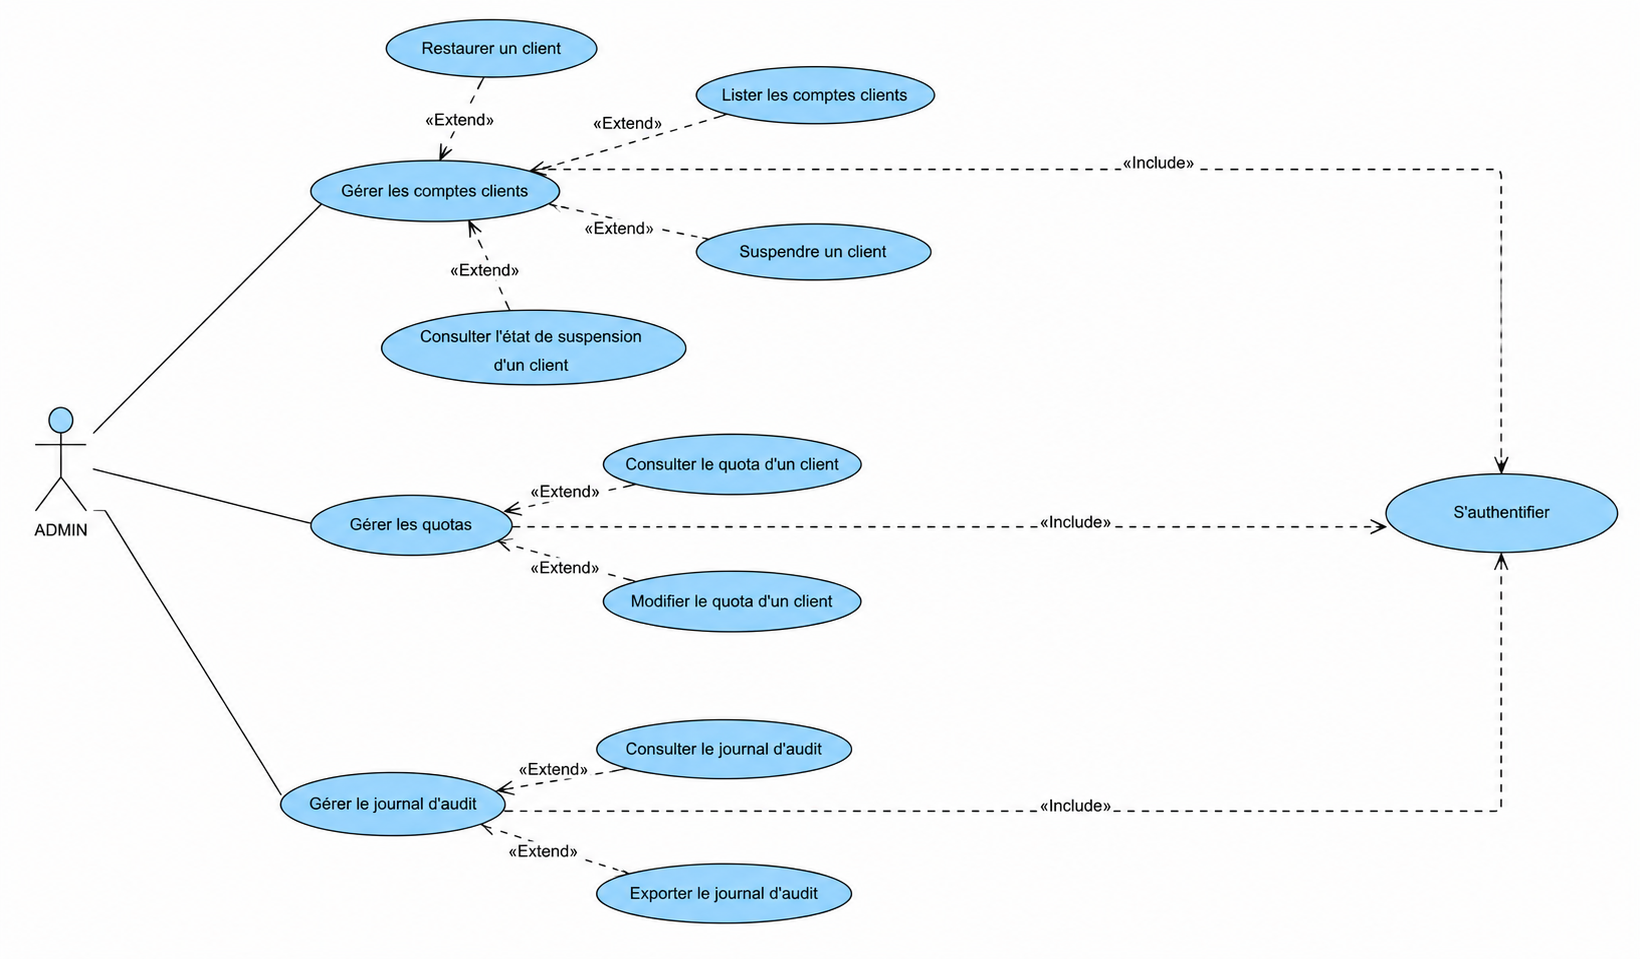
\includegraphics[width=\textwidth]{image/ucsprint8.png}
    \caption{Diagramme de cas d'utilisation du Sprint 8 — Comptes clients, quotas et audit}
    \label{fig:uc-sprint8}
\end{figure}
\subsection{Services Web}
{\setlength{\tabcolsep}{8pt}
\begin{longtable}{|p{5.8cm}|p{8.4cm}|}
\hline
Service Web & Description \\
\hline
\endfirsthead
\hline
Service Web & Description \\
\hline
\endhead
\endfoot
\hline
\endlastfoot
\texttt{GET\slash api\slash admin\slash clients} & Lister les comptes clients avec leur état de suspension. \\ \hline
\texttt{POST\slash api\slash admin\slash clients\slash\{userId\}\slash suspend} & Suspendre un compte client. \\ \hline
\texttt{POST\slash api\slash admin\slash clients\slash\{userId\}\slash restore} & Réactiver un compte client. \\ \hline
\texttt{GET\slash api\slash admin\slash clients\slash\{userId\}\slash quota} & Consulter le quota d'un client. \\ \hline
\texttt{PUT\slash api\slash admin\slash clients\slash\{userId\}\slash quota} & Modifier le quota d'un client. \\ \hline
\texttt{GET\slash api\slash admin\slash audit-log} & Consulter le journal d'audit, paginé et filtrable. \\ \hline
\texttt{GET\slash api\slash admin\slash audit-log\slash export} & Exporter le journal d'audit (CSV). \\ \hline
\end{longtable}}
% \subsection{Services Web}

% \needspace{0.55\textheight}
% {\setlength{\tabcolsep}{8pt}
% \begin{longtable}{|p{5.8cm}|p{8.4cm}|}
% \hline
% Service Web & Description \\
% \hline
% \endfirsthead
% \hline
% Service Web & Description \\
% \hline
% \endhead
% \endfoot
% \hline
% \endlastfoot
% \texttt{GET /api/admin/clients} & Lister les comptes clients avec leur état de suspension. \\ \hline
% \texttt{POST /api/admin/clients/\{userId\}/suspend} & Suspendre un compte client. \\ \hline
% \texttt{POST /api/admin/clients/\{userId\}/restore} & Réactiver un compte client. \\ \hline
% \texttt{GET /api/admin/clients/\{userId\}/quota} & Consulter le quota d'un client. \\ \hline
% \texttt{PUT /api/admin/clients/\{userId\}/quota} & Modifier le quota d'un client. \\ \hline
% \texttt{GET /api/admin/audit-log} & Consulter le journal d'audit, paginé et filtrable. \\ \hline
% \texttt{GET /api/admin/audit-log/export} & Exporter le journal d'audit (CSV). \\ \hline
% \end{longtable}}

\subsection{Conception}

Deux fonctionnalités sont détaillées : la suspension d'un compte client, l'action de gouvernance la plus significative de ce sprint ; la consultation du journal d'audit, qui trace précisément ce type d'action.

\needspace{0.45\textheight}
\subsubsection{Cas d'utilisation : « Suspendre un compte client »}

\subsubsection*{Description textuelle}

\renewcommand{\arraystretch}{1.5}
\begin{longtable}{|p{4cm}|p{11cm}|}
\hline
Nom & Suspendre un compte client \\
\hline
Acteur & ADMIN \\
\hline
Pré-condition & Le compte client existe et n'est pas déjà suspendu \\
\hline
Scénario nominal & 1. L'ADMIN sélectionne un compte client depuis la console d'administration. 2. Il déclenche la suspension. 3. Le backend suspend l'ensemble des services du client. 4. L'action est journalisée dans le journal d'audit. \\
\hline
Post-condition & Les services du client sont suspendus, l'action est tracée. \\
\hline
\caption{Description textuelle du cas d'utilisation « Suspendre un compte client »}
\label{tab:uc-suspend-client}
\end{longtable}

\needspace{0.35\textheight}
\subsubsection*{Diagramme de séquence}

\begin{figure}[H]
 \centering
    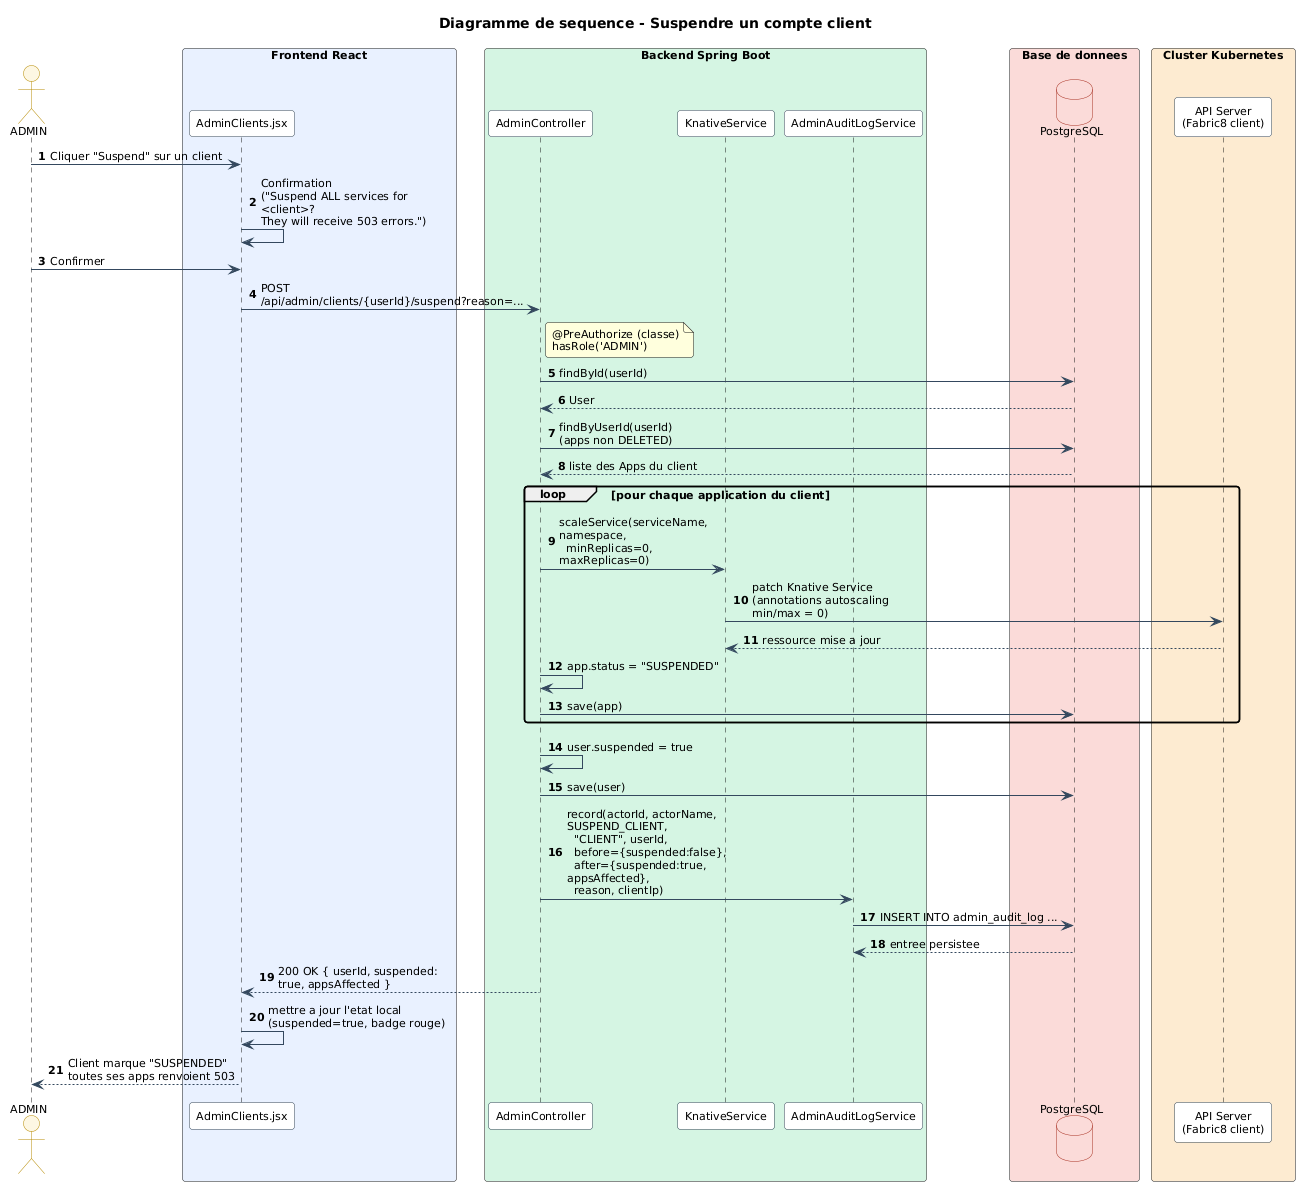
\includegraphics[width=0.9\textwidth]{image/secanse8suspendeapp.png}
    \caption{Diagramme de séquence — Suspendre un compte client}
    \label{fig:seq-suspend}
\end{figure}

\subsection{Réalisation du Sprint 8}

Fonctionnalité : Gérer les comptes clients — suspension, réactivation et quotas. La console d'administration liste les comptes clients avec leur état, permet de les suspendre ou de les réactiver, et de consulter/modifier leur quota de ressources (CPU, mémoire, nombre maximal d'applications), propagé au cluster.

\begin{figure}[H]
 \centering
    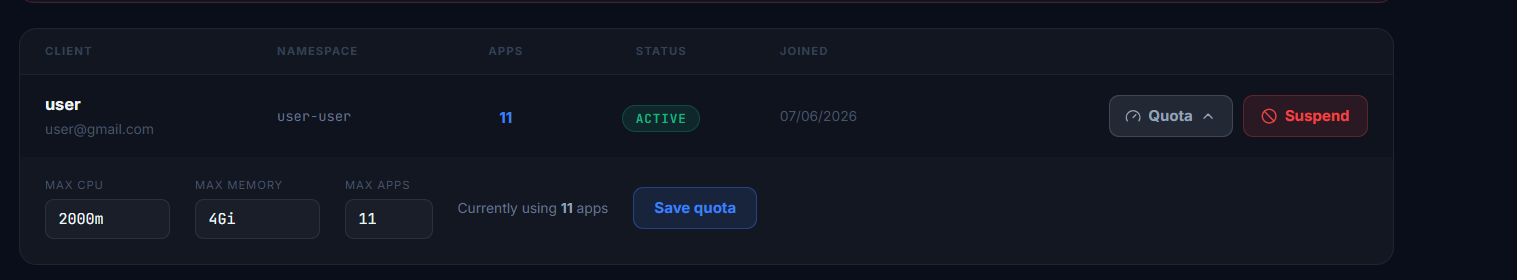
\includegraphics[width=0.9\textwidth]{image/Interface de gestion des quotas .png}
    \caption{Gestion des comptes clients}
    \label{fig:capture-quota}
\end{figure}

Fonctionnalité : Consulter et exporter le journal d'audit. Le journal d'audit liste les actions administratives sensibles, filtrables et exportables.

\begin{figure}[H]
 \centering
    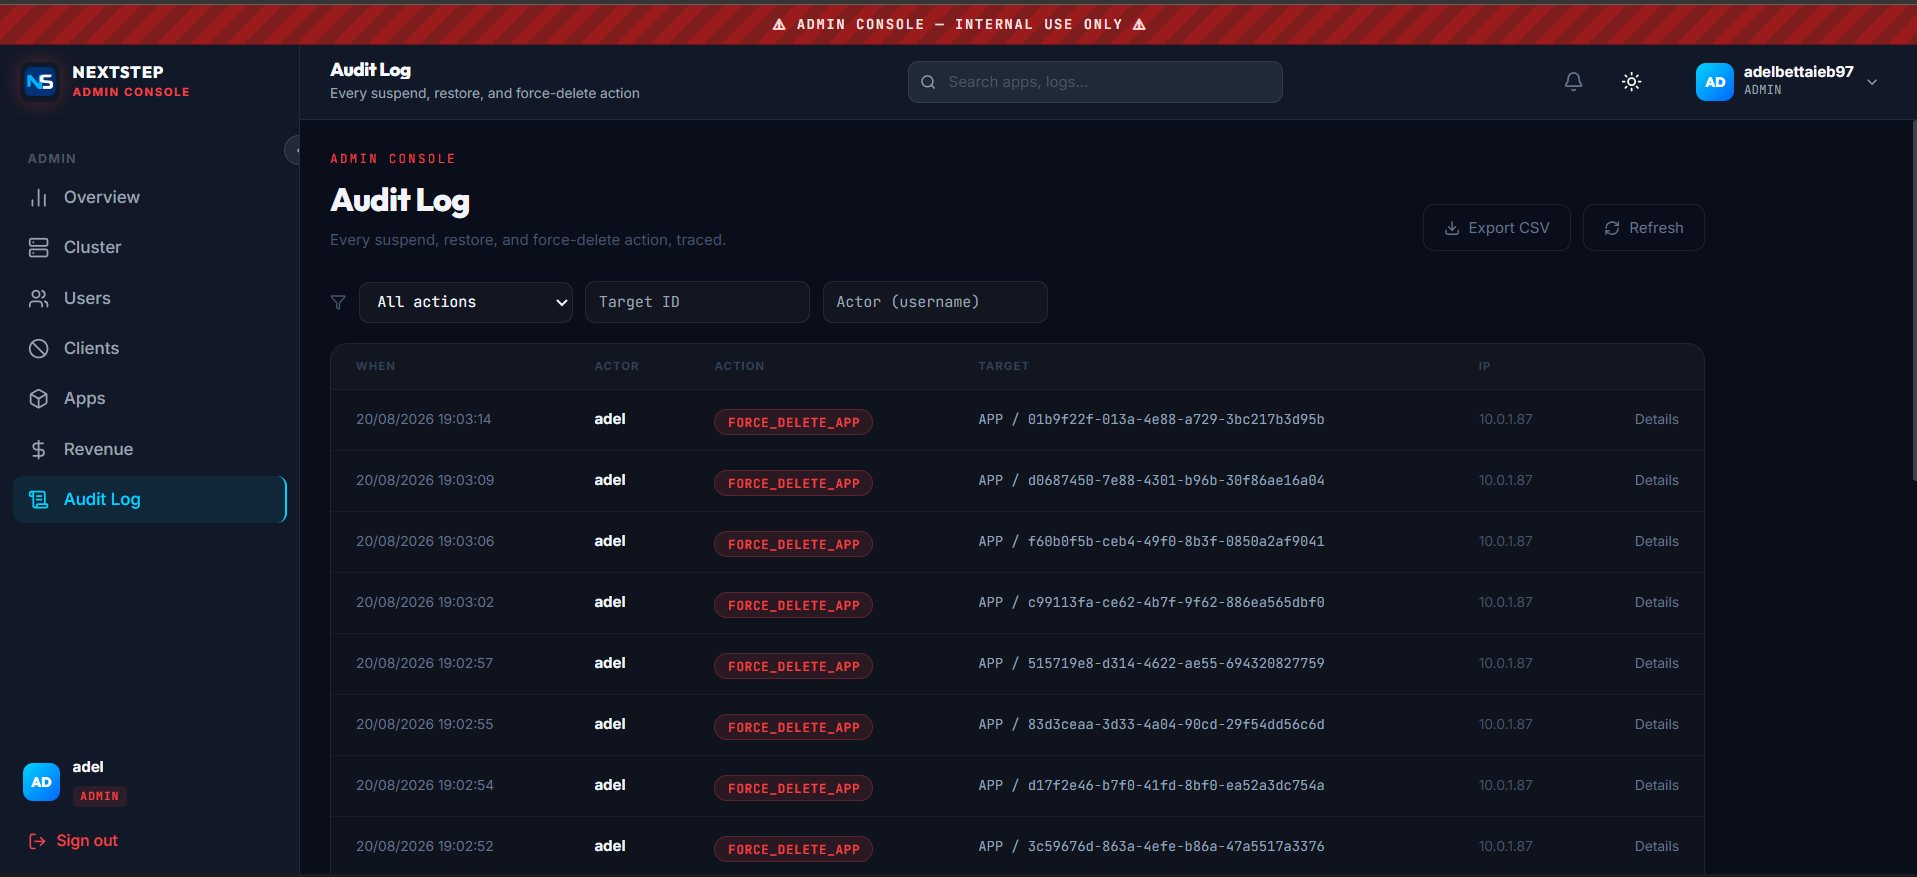
\includegraphics[width=0.9\textwidth]{image/Interface du journal d'audit.png}
    \caption{Interface du journal d'audit}
    \label{fig:capture-auditlog}
\end{figure}

Les actions tracées sont limitées à huit types : suspension et réactivation d'un compte client, suspension, réactivation, suppression forcée et redimensionnement d'une application, suppression forcée d'un sujet Kafka, et modification d'un quota. Le journal d'audit ne trace donc que la gouvernance administrative, jamais les consultations.

\subsection{Conclusion}

Ce sprint donne à l'ADMIN les leviers de gouvernance des comptes clients, avec une traçabilité systématique de leur usage. Il complète, sur le plan administratif, ce que le Sprint 9 complète sur le plan de la supervision technique du cluster.


\section{Sprint 9 : Gestion de l'exploitation du cluster et du statut public}

\subsection{Introduction}

Ce sprint dote l'ADMIN d'une supervision complète de l'état du cluster Kubernetes, et expose au public une page de statut synthétique de la disponibilité de la plateforme. Les deux fonctionnalités s'appuient sur la même donnée de santé du cluster, l'une en détail et en interne, l'autre de façon synthétique et publique.

\subsection{Sprint Backlog}

Le tableau~\ref{tab:sb-sprint9} présente le backlog détaillé du Sprint 9, obtenu en décomposant chaque User Story retenue en tâches techniques.

{
\setlength{\LTleft}{-1.5cm}
\setlength{\LTright}{-1.5cm}
\setlength{\tabcolsep}{8pt}
\renewcommand{\arraystretch}{1.9}
\begin{longtable}{|p{6.6cm}|>{\raggedright\arraybackslash}p{8.1cm}|>{\centering\arraybackslash}p{2.3cm}|}
\hline
User Story & Tâches & Estimation \\
\hline
\endfirsthead
\hline
User Story & Tâches & Estimation \\
\hline
\endhead
\endfoot
\hline

\caption{Backlog du Sprint 9}
\label{tab:sb-sprint9}
\endlastfoot

\multirow{3}{6.6cm}{\centering En tant qu'ADMIN, je veux consulter l'état complet du cluster Kubernetes afin de superviser l'infrastructure.}
& Développer la consultation des nœuds, pods, namespaces et volumes. & 2 \\ \cline{2-3}
& Développer la consultation des services Knative et des courtiers Kafka. & 2 \\ \cline{2-3}
& Développer la vue d'ensemble consolidée du cluster. & 2 \\ \hline

\multirow{3}{6.6cm}{\centering En tant qu'ADMIN, je veux consulter les alertes et les événements du cluster afin de détecter rapidement les incidents.}
& Développer la consultation des alertes actives. & 1 \\ \cline{2-3}
& Développer la consultation des événements d'avertissement récents. & 1 \\ \cline{2-3}
& Développer la santé des composants système. & 1 \\ \hline

\end{longtable}
}

\subsection{Diagramme de cas d'utilisation du Sprint 9}

Le diagramme réunit l'ADMIN (supervision détaillée du cluster) et le Public non authentifié (statut synthétique), ce dernier accès restant également ouvert aux trois autres rôles une fois connectés.

\begin{figure}[H]
 \centering
    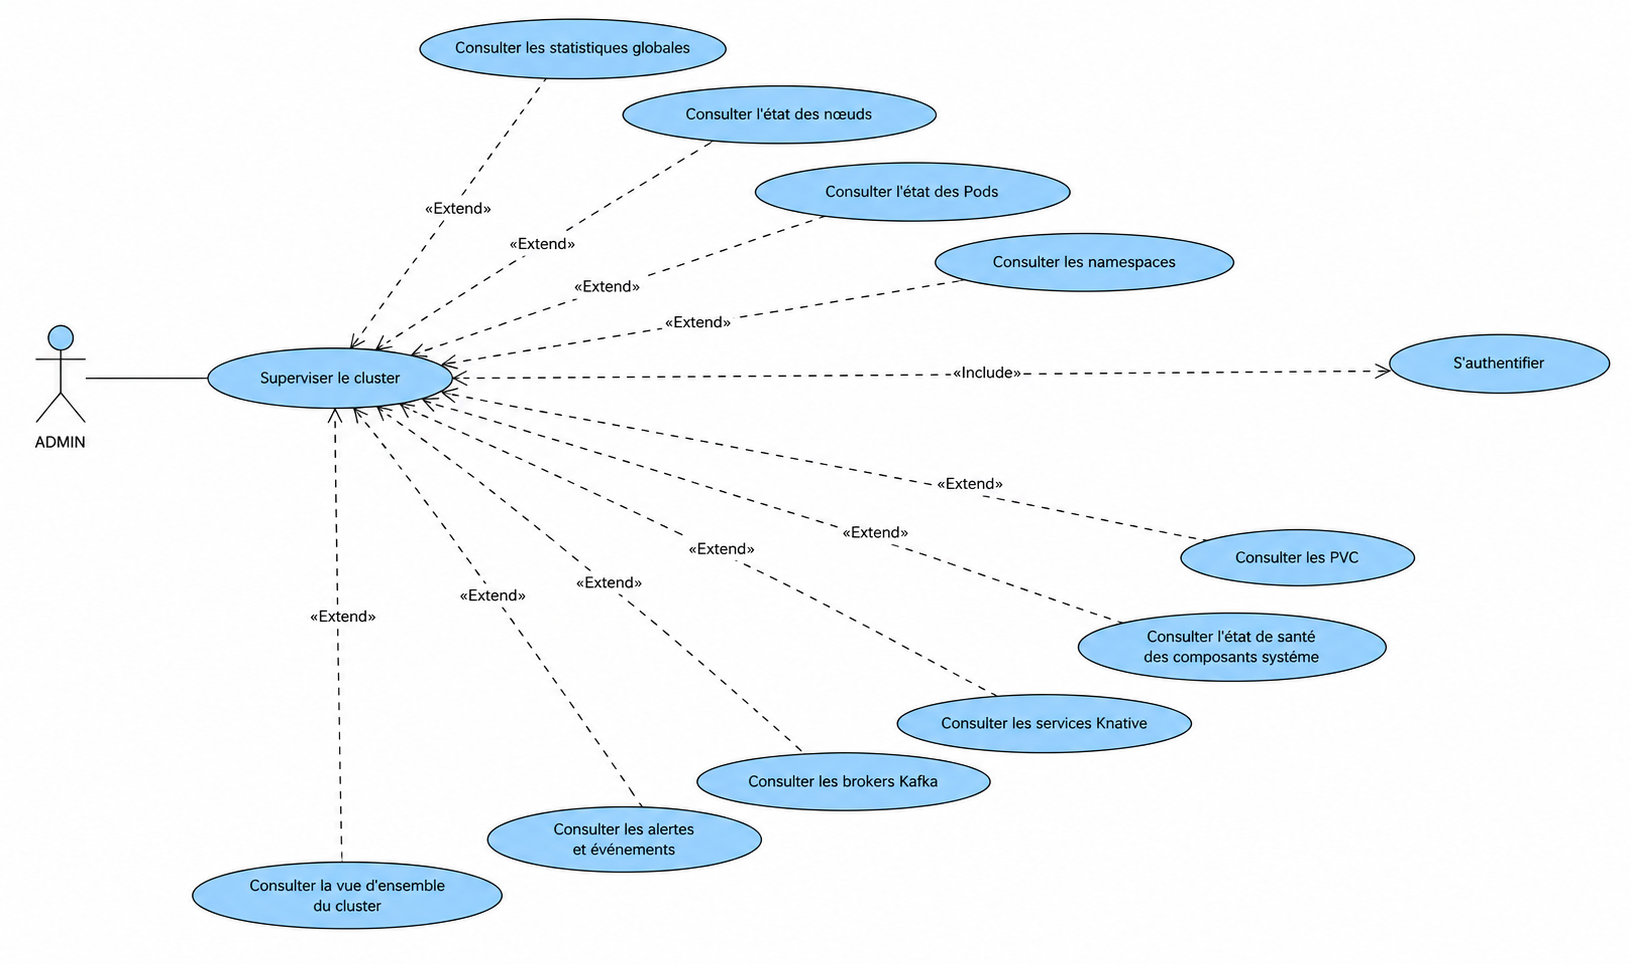
\includegraphics[width=\textwidth]{image/uc9.png}
    \caption{Diagramme de cas d'utilisation du Sprint 9 — Exploitation du cluster et statut public}
    \label{fig:uc-sprint9}
\end{figure}
\subsection{Services Web}
{\setlength{\tabcolsep}{8pt}
\begin{longtable}{|p{5.8cm}|p{8.4cm}|}
\hline
Service Web & Description \\
\hline
\endfirsthead
\hline
Service Web & Description \\
\hline
\endhead
\endfoot
\hline
\endlastfoot
\texttt{GET\slash api\slash admin\slash stats} & Statistiques globales de la plateforme (ADMIN). \\ \hline
\texttt{GET\slash api\slash admin\slash cluster\slash nodes}, \texttt{\slash namespaces}, \texttt{\slash pods}, \texttt{\slash storage} & État des nœuds, espaces de noms, pods et volumes (ADMIN). \\ \hline
\texttt{GET\slash api\slash admin\slash cluster\slash knative\slash services}, \texttt{\slash kafka\slash brokers} & État des services Knative et des courtiers Kafka (ADMIN). \\ \hline
\texttt{GET\slash api\slash admin\slash cluster\slash alerts}, \texttt{\slash events} & Alertes actives et événements d'avertissement récents (ADMIN). \\ \hline
\texttt{GET\slash api\slash admin\slash cluster\slash system-components} & Santé des composants système (ADMIN). \\ \hline
\texttt{GET\slash api\slash admin\slash cluster\slash overview} & Vue d'ensemble consolidée du cluster (ADMIN). \\ \hline
\texttt{GET\slash api\slash metrics\slash cluster} & Métriques agrégées du cluster (ADMIN). \\ \hline
\end{longtable}}
% \subsection{Services Web}

% \needspace{0.55\textheight}
% {\setlength{\tabcolsep}{8pt}
% \begin{longtable}{|p{5.8cm}|p{8.4cm}|}
% \hline
% Service Web & Description \\
% \hline
% \endfirsthead
% \hline
% Service Web & Description \\
% \hline
% \endhead
% \endfoot
% \hline
% \endlastfoot
% \texttt{GET /api/admin/stats} & Statistiques globales de la plateforme (ADMIN). \\ \hline
% \texttt{GET /api/admin/cluster/nodes}, \texttt{/namespaces}, \texttt{/pods}, \texttt{/storage} & État des nœuds, espaces de noms, pods et volumes (ADMIN). \\ \hline
% \texttt{GET /api/admin/cluster/knative/services}, \texttt{/kafka/brokers} & État des services Knative et des courtiers Kafka (ADMIN). \\ \hline
% \texttt{GET /api/admin/cluster/alerts}, \texttt{/events} & Alertes actives et événements d'avertissement récents (ADMIN). \\ \hline
% \texttt{GET /api/admin/cluster/system-components} & Santé des composants système (ADMIN). \\ \hline
% \texttt{GET /api/admin/cluster/overview} & Vue d'ensemble consolidée du cluster (ADMIN). \\ \hline
% \texttt{GET /api/metrics/cluster} & Métriques agrégées du cluster (ADMIN). \\ \hline
% \end{longtable}}

\subsection{Conception}

Deux fonctionnalités sont détaillées : la supervision du cluster, cœur du sprint côté ADMIN ; le statut public, fonctionnalité livrée dans le code mais jusqu'ici absente de ce mémoire.

\needspace{0.45\textheight}
\subsubsection{Cas d'utilisation : « Superviser le cluster »}

\subsubsection*{Description textuelle}

\renewcommand{\arraystretch}{1.5}
\begin{longtable}{|p{4cm}|p{11cm}|}
\hline
Nom & Superviser le cluster \\
\hline
Acteur & ADMIN \\
\hline
Pré-condition & L'ADMIN est authentifié sur la console d'administration \\
\hline
Scénario nominal & 1. L'ADMIN ouvre la page de supervision du cluster. 2. Le backend consulte l'API Kubernetes (nœuds, pods, espaces de noms) et Alertmanager (alertes actives). 3. L'état du cluster et les alertes actives sont affichés. \\
\hline
Post-condition & L'ADMIN dispose d'une vue à jour de l'état global du cluster. \\
\hline
\caption{Description textuelle du cas d'utilisation « Superviser le cluster »}
\label{tab:uc-cluster}
\end{longtable}

\needspace{0.35\textheight}
\subsubsection*{Diagramme de séquence}


\begin{figure}[H]
 \centering
    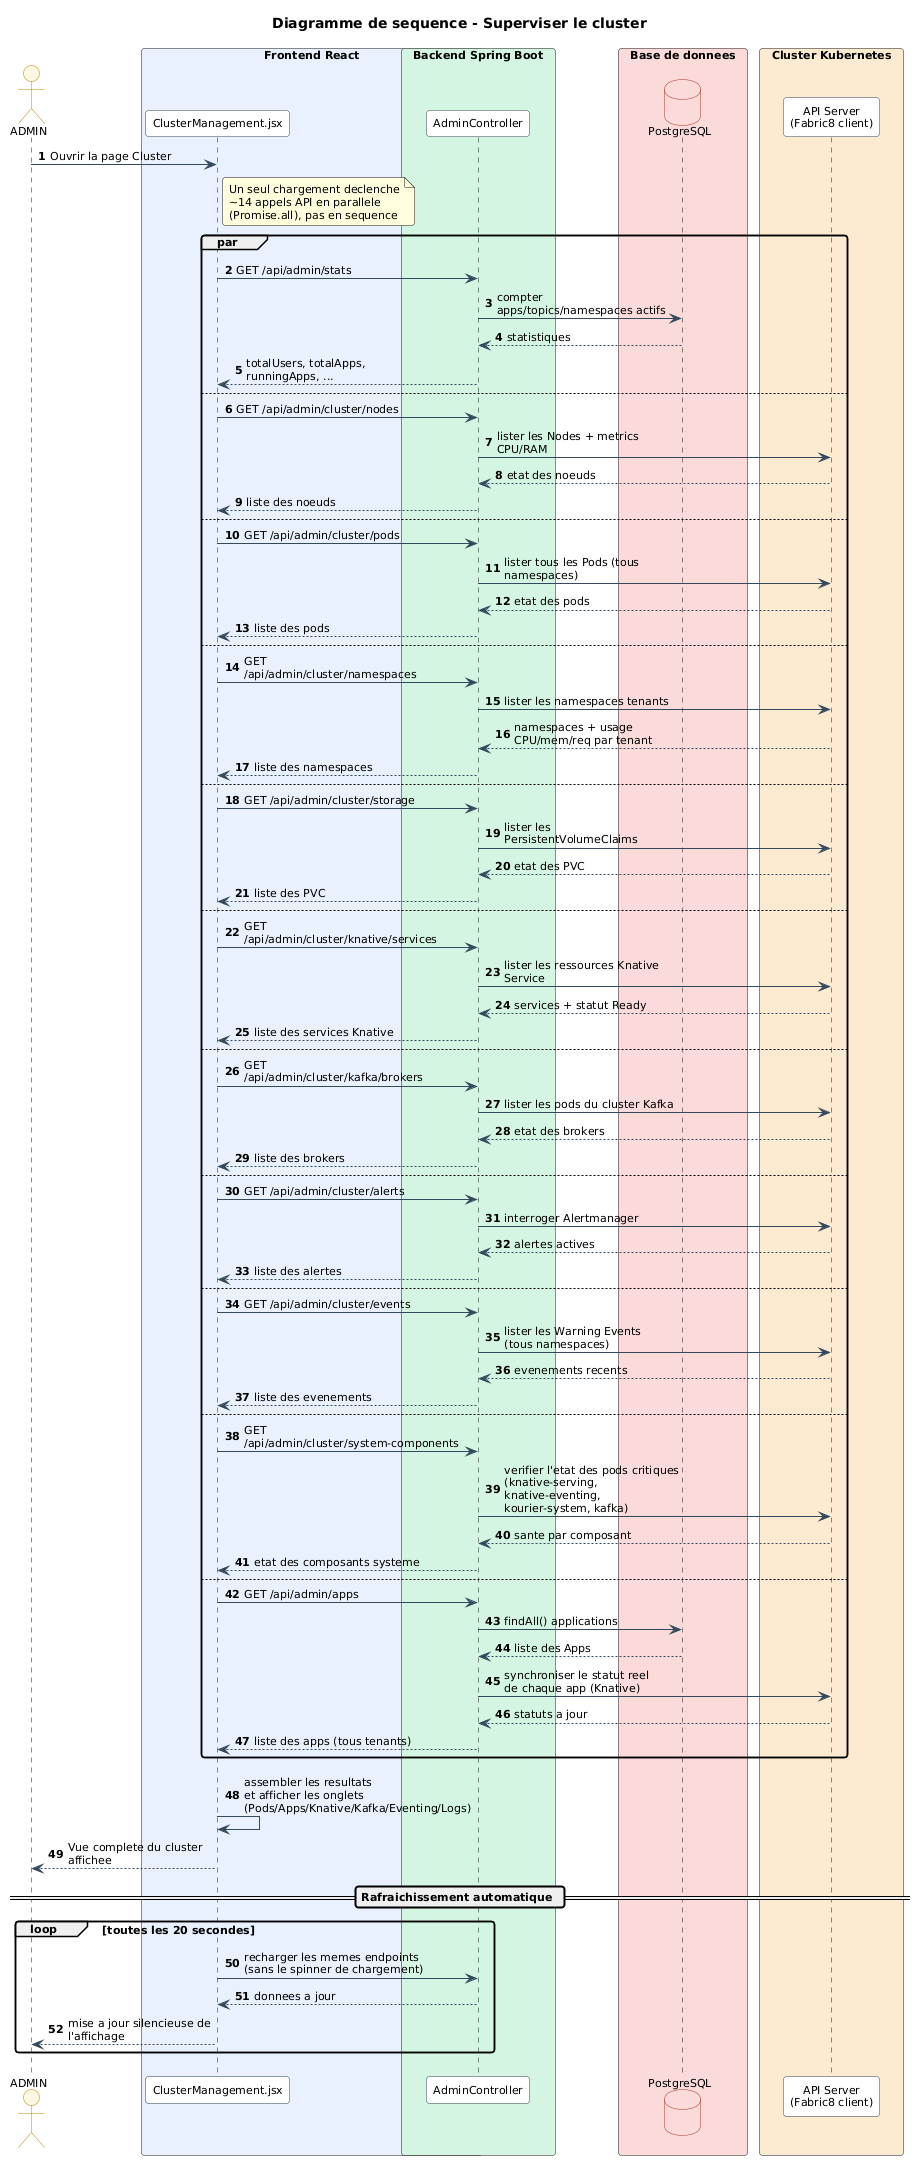
\includegraphics[width=0.9\textwidth]{image/seq-cluster.png}
    \caption{Diagramme de séquence — Superviser le cluster}
    \label{fig:seq-cluster}
\end{figure}

\subsection{Réalisation du Sprint 9}

Fonctionnalité : Superviser le cluster. La console d'administration affiche l'état des nœuds, des pods et des alertes actives du cluster.

\begin{figure}[H]
 \centering
    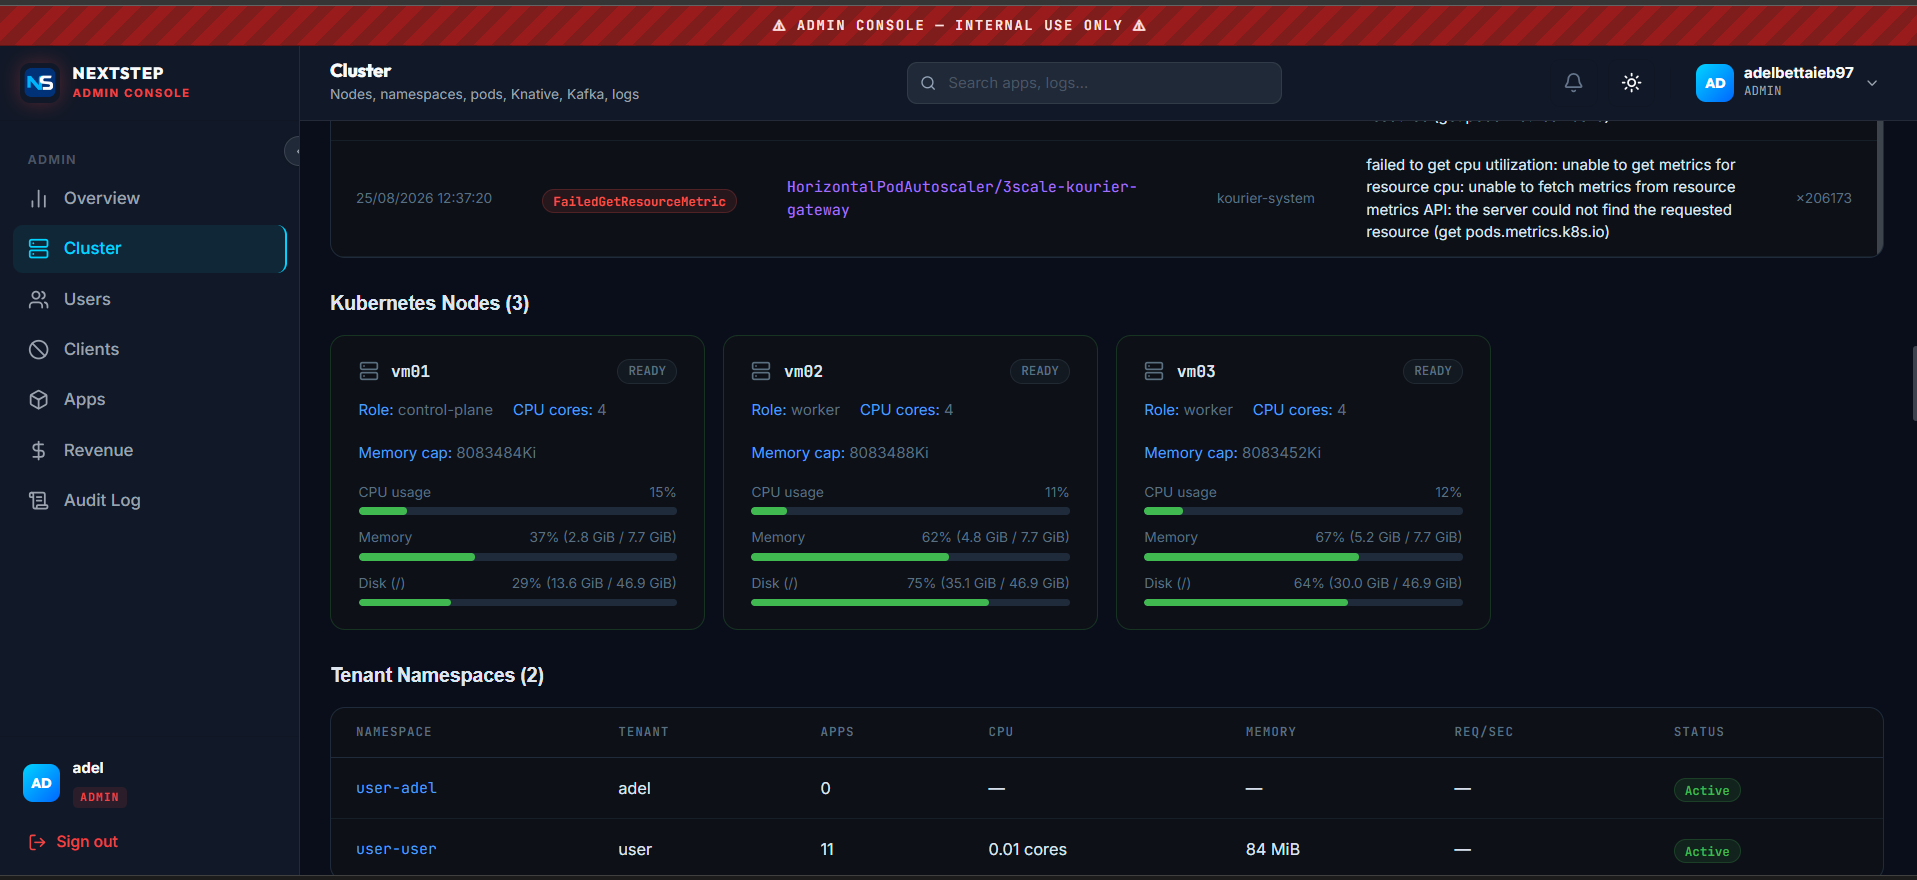
\includegraphics[width=0.9\textwidth]{image/Interface de supervision du cluster.png}
    \caption{Interface de supervision du cluster}
    \label{fig:capture-cluster}
\end{figure}

Fonctionnalité : Consulter les alertes et événements du cluster. Les alertes Alertmanager actives et les événements d'avertissement récents sont consultables depuis la même console.

\begin{figure}[H]
 \centering
    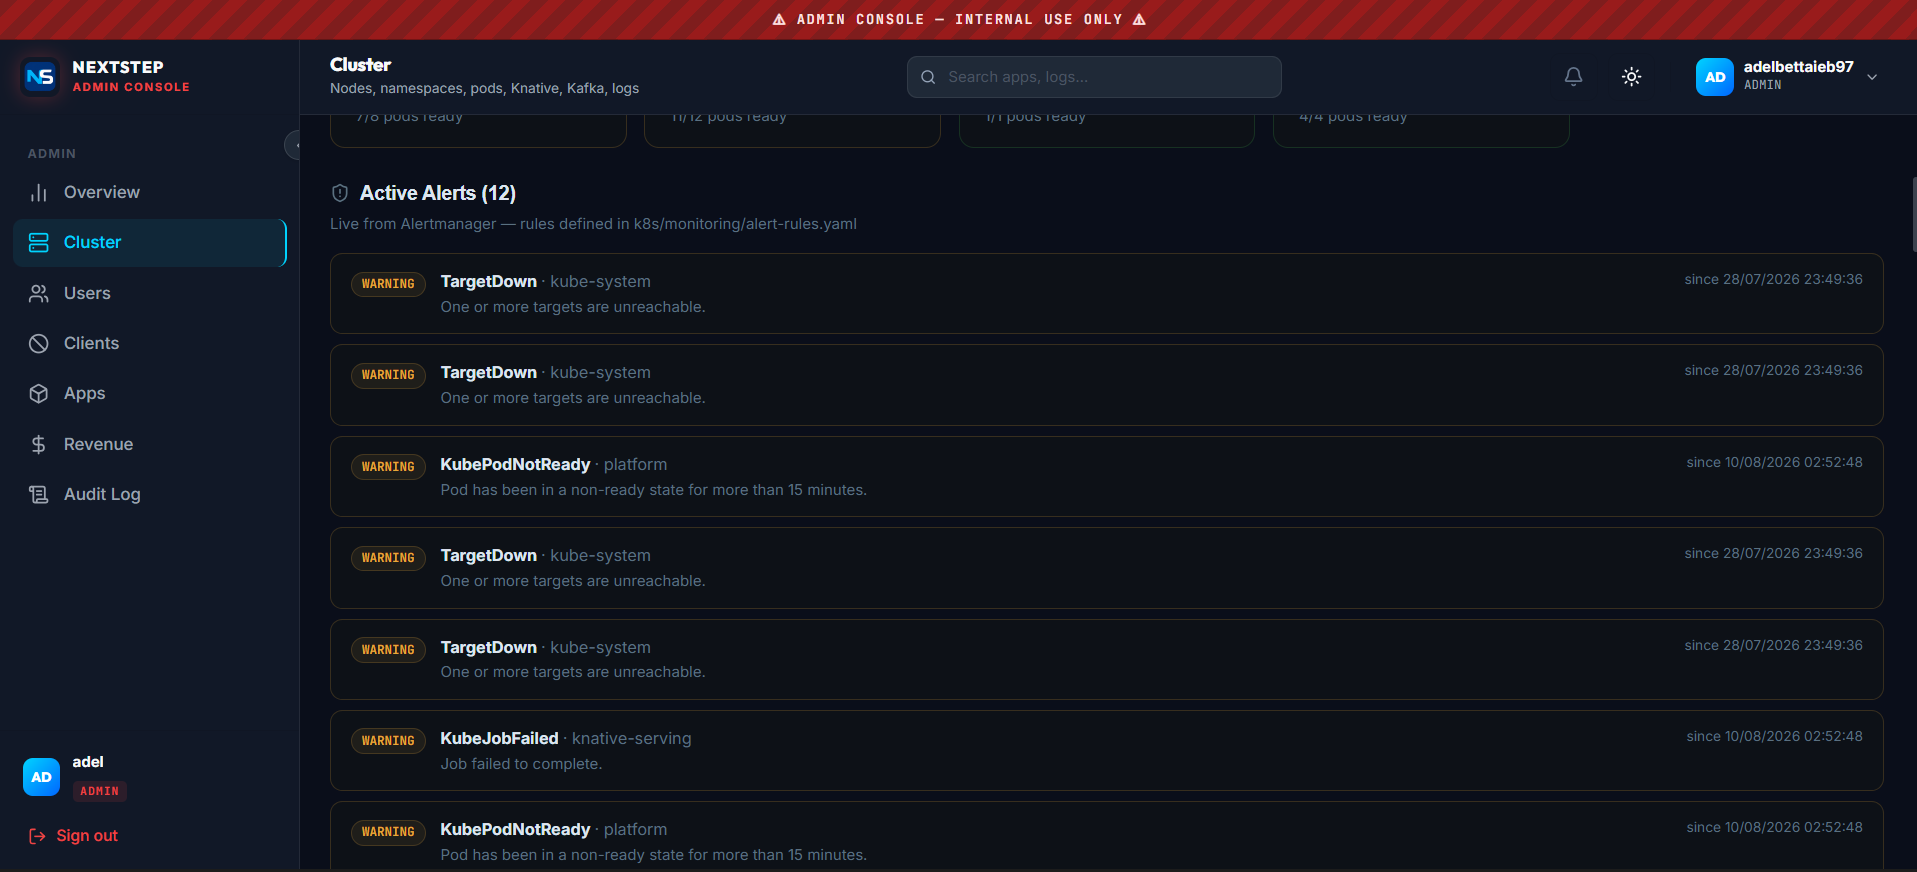
\includegraphics[width=0.9\textwidth]{image/Interface des alertes et événements du clust.png}
    \caption{Interface des alertes et événements du cluster}
    \label{fig:capture-alerts}
\end{figure}

\subsection{Conclusion}

Ce sprint clôt la Release 2 avec une supervision technique complète du cluster côté ADMIN, et une transparence de disponibilité offerte au public. La plateforme dispose désormais de l'ensemble des capacités de gestion applicative, de facturation et de supervision nécessaires à son exploitation par l'équipe de NextStep IT.

\section{Conclusion}

La Release 2 a complété la plateforme du point de vue de son exploitant : une facturation à l'usage mesurée automatiquement et réglable en ligne, une gouvernance des comptes clients tracée par un journal d'audit, et une supervision du cluster doublée d'une page de statut public. Comme pour la Release 1, plusieurs anomalies concrètes ont été identifiées et corrigées, et certaines limites ont été sciemment reportées, dans un contexte de ressources et de délai contraints, plutôt que dissimulées.


\chapter{Release 3 : Industrialisation}

\section{Introduction}

Les releases précédentes ont livré l'ensemble des capacités fonctionnelles de la plateforme, backend et interfaces graphiques confondus, pour les trois acteurs identifiés (CLIENT\_ADMIN, MEMBER, ADMIN). Cette dernière release, avant le chapitre de validation, ne porte plus sur des fonctionnalités nouvelles mais sur la solidité technique de la plateforme : consolider les mesures de sécurité mises en place au fil des sprints précédents (Sprint 10), puis harmoniser et fiabiliser les chaînes d'intégration continue de l'ensemble de ses composants (Sprint 11).

\clearpage
\section{Sprint 10 : Durcissement et sécurité}

\subsection{Introduction}

Ce sprint a pour objectif de consolider, en un point unique, les mesures de sécurité mises en place au fil des sprints précédents, et d'en ajouter quelques-unes supplémentaires identifiées lors d'une relecture transversale du projet, en amont de l'audit de sécurité formel présenté au chapitre de validation. Il ne s'agit pas d'un audit noté, mais d'un travail de durcissement technique mené par l'équipe de développement elle-même.

\subsection{Objectifs du Sprint}

\begin{itemize}
    \item Vérifier et compléter les rôles Kubernetes (RBAC) du backend, au-delà des extensions déjà apportées ponctuellement (Sprint 3, Sprint 9).
    \item Restreindre la configuration CORS du backend à une liste explicite d'origines autorisées.
    \item Identifier et corriger les accès non contrôlés à des ressources appartenant à d'autres tenants (IDOR) sur les points d'accès les plus sensibles.
    \item Documenter, sans les corriger si le délai du projet ne le permet pas, les risques résiduels identifiés, pour reprise explicite au chapitre de validation.
\end{itemize}

\subsection{Sprint Backlog}

Le tableau~\ref{tab:sb-sprint10} présente le backlog détaillé du Sprint 10, obtenu en décomposant chaque User Story retenue en tâches techniques.

% \needspace garantit qu'il reste assez de place sur la page : sans cela une
% coupure peut tomber au milieu d'un groupe \multirow, dont le contenu deborde
% alors hors du cadre et laisse une cellule vide sur la page suivante.
\needspace{0.9\textheight}
{
% Le tableau deborde volontairement de 1,5 cm dans chaque marge afin de laisser
% respirer les trois colonnes ; LTleft/LTright sont les parametres propres a
% longtable (adjustwidth n'a aucun effet sur cet environnement).
% Largeur totale : 18,8 cm, soit 1 cm de blanc conserve de chaque cote de la page.
\setlength{\LTleft}{-1.5cm}
\setlength{\LTright}{-1.5cm}
\setlength{\tabcolsep}{8pt}
\renewcommand{\arraystretch}{1.9}
\begin{longtable}{|p{6.6cm}|>{\raggedright\arraybackslash}p{8.1cm}|>{\centering\arraybackslash}p{2.3cm}|}
\hline
User Story & Tâches & Estimation \\
\hline
\endfirsthead
\hline
User Story & Tâches & Estimation \\
\hline
\endhead
\hline
\endfoot

\caption{Backlog du Sprint 10}
\label{tab:sb-sprint10}
\endlastfoot

\multirow{1}{6.6cm}{
\centering
En tant qu'exploitant, je veux que le \texttt{ClusterRole} du backend soit limité aux permissions réellement nécessaires.
}
&
Reconstruire le \texttt{ClusterRole} à partir des ressources effectivement manipulées, vérifier avec \texttt{kubectl auth can-i}.
& — \\
\hline

\multirow{1}{6.6cm}{
\centering
En tant qu'exploitant, je veux restreindre les origines autorisées à appeler l'API.
}
&
Configurer \texttt{app.cors.allowed-origins} en liste explicite.
& — \\
\hline

\multirow{1}{6.6cm}{
\centering
En tant qu'exploitant, je veux qu'un client ne puisse pas accéder aux ressources d'un autre tenant par manipulation d'identifiant.
}
&
Auditer et corriger les accès directs par identifiant sur les points d'accès sensibles (journaux, moyens de paiement).
& — \\
\hline

\end{longtable}
}

\subsection{Conception}

\subsubsection{Synthèse des mesures de durcissement}

Plusieurs mesures de sécurité ont déjà été introduites au fil des sprints précédents, à mesure que les anomalies correspondantes étaient identifiées : reconstruction du \texttt{ClusterRole} du backend (Sprint 3), migration du jeton d'authentification hors des paramètres d'URL du flux de journaux (Sprint 3), correction de la référence au rôle ADMIN dans la facturation (Sprint 7), extension du \texttt{ClusterRole} à la lecture des nœuds et événements pour la console d'administration (Sprint 9). Ce sprint reprend ces mesures dans une démarche volontairement transversale, plutôt que de les laisser dispersées au fil des sprints fonctionnels, et y ajoute la restriction CORS et la revue des accès directs par identifiant (IDOR).

\subsubsection{Configuration CORS}

Le backend restreint les origines autorisées à une liste explicite, portée par la propriété \texttt{app.cors.allowed-origins}, plutôt qu'un caractère générique. Cette configuration autorise l'envoi des identifiants de session (\texttt{allowCredentials}) uniquement pour les origines listées, et limite les méthodes HTTP acceptées à celles réellement utilisées par l'API (\texttt{GET}, \texttt{POST}, \texttt{PUT}, \texttt{PATCH}, \texttt{DELETE}, \texttt{OPTIONS}).

\subsection{Réalisation}

\subsubsection{Mise en œuvre}

La revue des points d'accès manipulant une ressource par identifiant (journaux de déploiement, moyens de paiement enregistrés) a permis de vérifier, ou le cas échéant de corriger, que chaque accès est bien filtré par l'identité effective de l'appelant, résolue par \texttt{UserContextService}, plutôt que par le seul identifiant transmis dans l'URL.

\subsubsection{Configuration et limites assumées}

Ce sprint ne prétend pas clore la question de la sécurité de la plateforme : il s'agit d'une étape de durcissement technique, dont le résultat mesuré (score de sécurité avant/après) est présenté formellement au chapitre de validation, avec la liste complète des vulnérabilités traitées ou assumées comme risque produit. Certains points, en particulier l'absence de limite de ressources par défaut par tenant et le flux d'authentification Resource Owner Password Credentials du portail (Sprint 3), ne sont pas traités dans ce sprint et restent des risques assumés.

Au terme de ce sprint, les principales mesures de durcissement identifiées au fil du projet sont consolidées ; le chapitre de validation qui suit en mesure formellement l'effet sur la posture de sécurité globale de la plateforme. Ce sprint ne couvre pas l'ensemble des vulnérabilités possibles : l'absence de limite de ressources par défaut par tenant et le flux d'authentification ROPC du portail restent des risques produit assumés, documentés au chapitre de validation.

\clearpage
\section{Sprint 11 : Pipeline CI/CD complet}

\subsection{Introduction}

Ce sprint a pour objectif de doter chacun des composants de la plateforme (backend, portail client, console d'administration) d'un pipeline d'intégration continue, puis de consolider et d'harmoniser ces pipelines sur un socle commun plus robuste, en généralisant les mécanismes de fiabilisation mis au point empiriquement lors du Sprint 4 pour le pipeline backend.

\subsection{Objectifs du Sprint}

\begin{itemize}
    \item Mettre en place un pipeline Jenkins pour le portail client et pour la console d'administration, sur le même principe que le pipeline backend (Sprint 4).
    \item Harmoniser les pipelines Jenkins existants sur un socle commun plus robuste.
    \item Fiabiliser l'exécution de Kaniko afin d'éviter les échecs de construction dus à la corruption de l'environnement Jenkins identifiée au Sprint 4.
    \item Clarifier l'usage des différents fichiers Dockerfile du backend, source de confusion identifiée lors de l'audit du projet.
\end{itemize}

\subsection{Sprint Backlog}

Le tableau~\ref{tab:sb-sprint11} présente le backlog détaillé du Sprint 11, obtenu en décomposant chaque User Story retenue en tâches techniques.

% \needspace garantit qu'il reste assez de place sur la page : sans cela une
% coupure peut tomber au milieu d'un groupe \multirow, dont le contenu deborde
% alors hors du cadre et laisse une cellule vide sur la page suivante.
\needspace{0.9\textheight}
{
% Le tableau deborde volontairement de 1,5 cm dans chaque marge afin de laisser
% respirer les trois colonnes ; LTleft/LTright sont les parametres propres a
% longtable (adjustwidth n'a aucun effet sur cet environnement).
% Largeur totale : 18,8 cm, soit 1 cm de blanc conserve de chaque cote de la page.
\setlength{\LTleft}{-1.5cm}
\setlength{\LTright}{-1.5cm}
\setlength{\tabcolsep}{8pt}
\renewcommand{\arraystretch}{1.9}
\begin{longtable}{|p{6.6cm}|>{\raggedright\arraybackslash}p{8.1cm}|>{\centering\arraybackslash}p{2.3cm}|}
\hline
User Story & Tâches & Estimation \\
\hline
\endfirsthead
\hline
User Story & Tâches & Estimation \\
\hline
\endhead
\hline
\endfoot

\caption{Backlog du Sprint 11}
\label{tab:sb-sprint11}
\endlastfoot

\multirow{2}{6.6cm}{
\centering
En tant qu'exploitant, je veux que le portail client et la console d'administration soient construits et déployés automatiquement.
}
&
Mettre en place le pipeline Jenkins portail (\texttt{npm run build}, Kaniko, Docker Hub).
& — \\
\cline{2-3}

&
Mettre en place le pipeline Jenkins admin-console.
& — \\
\hline

\multirow{2}{6.6cm}{
\centering
En tant qu'exploitant, je veux fiabiliser l'exécution du pipeline backend.
}
&
Ajouter un réessai automatique à l'étape Checkout.
& — \\
\cline{2-3}

&
Ajouter \texttt{--use-new-run}/\texttt{--snapshot-mode=redo} + redémarrage systématique de Jenkins.
& — \\
\hline

\multirow{1}{6.6cm}{
\centering
En tant qu'exploitant, je veux un pipeline unique et cohérent pour tous les composants.
}
&
Aligner les 4 pipelines sur le socle backend (non réalisé).
& — \\
\hline

\multirow{1}{6.6cm}{
\centering
En tant qu'exploitant, je veux une étape de tests automatisés dans les pipelines.
}
&
Retirer \texttt{-DskipTests} et ajouter une étape de test (non réalisé).
& — \\
\hline

\multirow{1}{6.6cm}{
\centering
En tant qu'exploitant, je veux une analyse de sécurité des images construites.
}
&
Intégrer un scanner de vulnérabilités dans le pipeline (non réalisé).
& — \\
\hline

\end{longtable}
}

\subsection{Conception}

La figure~\ref{fig:cicd-pipeline} illustre le pipeline backend, le plus complet des quatre à l'issue de ce sprint. L'étape Test y est représentée en pointillés : elle n'est pas réellement exécutée, la compilation Maven étant lancée avec l'option \texttt{-DskipTests} (cf. Réalisation ci-après), elle figure ici comme étape cible non atteinte, pas comme un fait acquis.

\begin{figure}[H]
\centering
\begin{tikzpicture}[node distance=1.1cm, every node/.style={font=\footnotesize}]
\tikzstyle{box}=[draw, rounded corners, minimum width=1.7cm, minimum height=0.8cm, align=center, fill=Gray!20]
\tikzstyle{boxdash}=[box, dashed, fill=Gray!5]
\node[box] (dev) {Developer};
\node[box, right=0.9cm of dev] (git) {Git};
\node[box, right=0.9cm of git] (jenkins) {Jenkins};
\node[box, right=0.9cm of jenkins] (checkout) {Checkout};
\node[box, right=0.9cm of checkout] (build) {Build\\(Maven)};
\node[boxdash, right=0.9cm of build] (test) {Test\\(non exécuté)};
\node[box, below=1.3cm of build] (kaniko) {Kaniko};
\node[box, right=0.9cm of kaniko] (registry) {Docker Hub};
\node[box, right=0.9cm of registry] (k8s) {Kubernetes};
\node[box, right=0.9cm of k8s] (rollout) {Rollout};
\node[box, right=0.9cm of rollout] (app) {Application};
\draw[->, thick] (dev) -- (git);
\draw[->, thick] (git) -- (jenkins);
\draw[->, thick] (jenkins) -- (checkout);
\draw[->, thick] (checkout) -- (build);
\draw[->, thick] (build) -- (test);
\draw[->, thick] (build) -- (kaniko);
\draw[->, thick] (kaniko) -- (registry);
\draw[->, thick] (registry) -- (k8s);
\draw[->, thick] (k8s) -- (rollout);
\draw[->, thick] (rollout) -- (app);
\end{tikzpicture}
\caption{Pipeline CI/CD backend : Developer $\rightarrow$ Git $\rightarrow$ Jenkins $\rightarrow$ Checkout $\rightarrow$ Build $\rightarrow$ Kaniko $\rightarrow$ Docker Hub $\rightarrow$ Kubernetes $\rightarrow$ Rollout $\rightarrow$ Application}
\label{fig:cicd-pipeline}
\end{figure}

\begin{table}[H]
\centering
\setlength{\tabcolsep}{4pt}
\renewcommand{\arraystretch}{1.5}
\begin{tabular}{|>{\raggedright\arraybackslash}p{2.3cm}|>{\raggedright\arraybackslash}p{2.4cm}|>{\raggedright\arraybackslash}p{3.1cm}|>{\raggedright\arraybackslash}p{3.1cm}|>{\raggedright\arraybackslash}p{3.4cm}|}
\hline
Étape & Outil & Entrée & Sortie & Validation \\
\hline
Checkout & Jenkins + Git (avec réessai) & Dépôt Git & Code source local & Réessai automatique si échec transitoire \\
\hline
Build & Maven (\texttt{mvn clean package}, \texttt{-DskipTests}) & Code source & Archive \texttt{.jar} & Compilation sans erreur (tests non exécutés) \\
\hline
Construction image & Kaniko (\texttt{--use-new-run}, \texttt{--snapshot-mode=redo}) & \texttt{.jar} + \texttt{backend-kaniko.Dockerfile} & Image de conteneur & Build Kaniko réussi \\
\hline
Publication & Docker Hub & Image construite & Image taguée disponible & Push réussi \\
\hline
Déploiement & \texttt{kubectl set image} & Nouvelle image publiée & Déploiement Kubernetes mis à jour & \texttt{kubectl rollout status} réussi \\
\hline
\end{tabular}
\caption{Étapes du pipeline CI/CD backend}
\label{tab:cicd-steps}
\end{table}

Les pipelines du portail client et de la console d'administration reprennent le même squelette, adapté à une application front-end : construction (\texttt{npm run build}) produisant les fichiers statiques, construction de l'image de conteneur (Nginx servant ces fichiers statiques) via Kaniko, publication sur Docker Hub, puis mise à jour du déploiement Kubernetes correspondant.

\subsection{Réalisation}

\subsubsection{Mise en œuvre}

Les correctifs de fiabilisation identifiés au Sprint 4 (options Kaniko \texttt{--use-new-run}/\texttt{--snapshot-mode=redo}, redémarrage sécurisé systématique de Jenkins, réessai automatique du checkout Git) demeurent, à l'issue de ce sprint, appliqués uniquement au pipeline du backend, qui reste le plus mature des quatre. Les pipelines du portail client et de la console d'administration, mis en place à ce sprint, permettent leur construction et leur déploiement automatisés, mais sans reprendre l'ensemble de ces mécanismes de fiabilisation. Le remplacement du fichier \texttt{backend.Dockerfile} (construction multi-étapes avec utilisateur non privilégié, non utilisé en pratique par le pipeline) au profit exclusif de \texttt{backend-kaniko.Dockerfile} (construction mono-étape effectivement utilisée) a été clarifié dans la documentation technique du projet, sans toutefois que le premier fichier, devenu du code mort, n'ait été supprimé du dépôt.

\subsubsection{Configuration et limites assumées}

En toute rigueur, ce sprint doit être présenté avec honnêteté au regard de son objectif initial : l'harmonisation complète des pipelines CI/CD n'a été que partiellement atteinte. Les points suivants, documentés par les audits menés sur la plateforme, n'ont pas été résolus dans le temps imparti du projet et sont repris comme perspectives d'amélioration au chapitre de validation :

\begin{itemize}
    \item Les pipelines du portail client et de la console d'administration n'ont pas été alignés sur les mécanismes de fiabilisation du pipeline backend.
    \item Le pipeline dédié aux microservices reste le moins abouti des quatre : construction et publication d'image Docker classiques (sans Kaniko), absence d'identifiants explicites pour le checkout Git, et absence de toute étape de déploiement Kubernetes final.
    \item Aucun des quatre pipelines ne comporte d'étape de tests automatisés (la compilation backend est réalisée avec l'option \texttt{-DskipTests}), d'analyse statique de code, ni d'analyse de vulnérabilités des images construites.
    \item Aucun mécanisme de rollback automatique n'est déclenché en cas d'échec de la vérification du déploiement (\texttt{kubectl rollout status}).
\end{itemize}

Ces limites ne remettent pas en cause le fonctionnement de la plateforme, qui reste opérationnelle et déployée automatiquement à chaque évolution ; elles constituent en revanche des axes d'industrialisation identifiés mais non traités, dans un contexte de projet à ressources et délai contraints, où la priorité a été donnée à la robustesse fonctionnelle de la plateforme elle-même plutôt qu'à l'homogénéisation complète de ses quatre pipelines.

Au terme de ce sprint, le pipeline backend demeure le plus robuste et le plus représentatif de la démarche CI/CD visée pour la plateforme ; les trois autres pipelines sont fonctionnels mais perfectibles. Les 3 autres pipelines (portail, admin, microservices) ne bénéficient pas des mêmes mécanismes de fiabilisation que le backend ; aucun des 4 pipelines n'exécute de tests automatisés, d'analyse statique, ni d'analyse de vulnérabilités ; aucun rollback automatique n'est déclenché en cas d'échec de déploiement. Ces limites sont assumées comme telles, dans un contexte de ressources et de délai contraints, et reprises au chapitre de validation.

\section{Conclusion}

La Release 3 a consolidé la solidité technique de la plateforme sans lui ajouter de nouvelle fonctionnalité visible : durcissement de la sécurité par la restriction du RBAC, de la configuration CORS et des accès par identifiant, puis industrialisation des chaînes de déploiement continu des quatre composants du projet. Ce travail d'industrialisation, présenté ici avec la même rigueur que les fonctionnalités abouties, n'a été que partiellement mené à son terme : ce constat, assumé, alimente directement le chapitre de validation qui clôt ce mémoire.


\chapter*{Conclusion Générale}
\addcontentsline{toc}{chapter}{Conclusion Générale}

Ce Projet de Fin d'Études, réalisé au sein de NextStep IT, avait pour objectif de concevoir et de réaliser une plateforme PaaS serverless multi-tenant, bâtie sur Kubernetes, permettant à des clients de déployer et d'exploiter des applications conteneurisées sans en gérer directement la complexité d'orchestration sous-jacente, avec une mise à l'échelle automatique jusqu'à zéro instance, une intégration native avec un système de messagerie événementielle, et une facturation reflétant l'usage réel des ressources.

La démarche suivie, structurée selon la méthodologie agile Scrum et organisée en quatre releases successives, a permis de construire cette plateforme de manière incrémentale et validée à chaque étape. La Release 0 a établi le socle Cloud Native du système : cluster Kubernetes isolé par tenant, exécution serverless via Knative Serving, messagerie événementielle via Kafka et Strimzi. La Release 1 a transformé ce socle en cœur applicatif cohérent, organisé par domaine de gestion : identité et contrôle d'accès, cycle de vie complet d'une application, messagerie événementielle exposée au client, et observabilité applicative. La Release 2 a ouvert la plateforme à son exploitation commerciale et opérationnelle : facturation à l'usage et paiement en ligne, gestion des comptes clients, des quotas et de l'audit, supervision du cluster et page de statut public. La Release 3, enfin, a consolidé la solidité technique de l'ensemble, par le durcissement de la sécurité et l'industrialisation des chaînes de déploiement continu.

Sur le plan technique, ce projet a permis de mettre en pratique, dans un contexte réel et contraint, un ensemble de technologies cloud native encore peu matures et en évolution rapide (Knative Serving, Knative Eventing, Strimzi) en les combinant à un backend Spring Boot orchestrant le cluster de manière programmatique via le client Fabric8, et à des interfaces React exploitant ces capacités au travers d'une API REST sécurisée. Il a également permis d'expérimenter concrètement les difficultés propres à l'intégration de briques d'infrastructure hétérogènes : cohérence entre l'état applicatif persisté et l'état réel du cluster, fiabilisation d'une chaîne d'intégration continue reposant sur la construction d'images sans démon privilégié, ou encore arbitrages entre sécurité idéale et contraintes de délai et de modèle produit.

Ce mémoire s'est attaché, à chaque étape, à documenter avec la même rigueur les fonctionnalités abouties et les limites identifiées, qu'il s'agisse de choix assumés ou de chantiers inachevés faute de temps. Ces limites, loin de constituer un aveu d'échec, dessinent une feuille de route réaliste pour une éventuelle industrialisation ultérieure de la plateforme par NextStep IT : généralisation de l'infrastructure-as-code à l'ensemble du socle cluster, migration du flux d'authentification vers Authorization Code avec PKCE, isolation renforcée du cluster Kafka partagé entre tenants, intégration de tests automatisés et d'une analyse de vulnérabilités dans les pipelines, et refactorisation de la duplication de code entre les deux applications frontend.

Au terme de ce projet, la problématique posée en introduction — permettre à des clients multiples de déployer de manière autonome et sécurisée des applications conteneurisées, avec une mise à l'échelle automatique incluant le retour à zéro instance, une intégration événementielle native et une facturation à l'usage — trouve une réponse fonctionnelle complète et opérationnelle, dont les limites ont été explicitement circonscrites. Ce travail constitue ainsi, pour NextStep IT, une base concrète et documentée pour l'évolution de son offre Cloud vers des services de plateforme applicative à plus forte valeur ajoutée.



% ============================================================
% BIBLIOGRAPHIE
% ============================================================

\nocite{*}

\printbibliography[
    title={Bibliographie}
]


% ============================================================
% PAGE DE FIN
% ============================================================


\includepdf[
    pages=-,
    pagecommand={\thispagestyle{empty}}
]{Page-de-garde/page_fin.pdf}

\clearpage

\thispagestyle{empty}


\end{document}